\documentclass [11pt,twoside]{report}
\pagestyle{plain}
\usepackage{geometry}
\geometry{a4paper,inner=40mm,outer=20mm,top=30mm,bottom=20mm}
\usepackage{setspace}
\onehalfspacing
\usepackage{caption}
\usepackage{subfig}
\usepackage{graphicx}
\usepackage{longtable}
\usepackage{rotating}
\usepackage{url}
\usepackage{aas_macros}
\usepackage{amsmath}
\usepackage{gensymb}
\usepackage[round]{natbib}
\bibliographystyle{natbib}
%\bibliographystyle{abbrvnat}
%\bibliographystyle{plainnat}
\usepackage{hyperref}
\usepackage[usenames,dvipsnames]{xcolor}
\usepackage{bold-extra}
\usepackage{amssymb}
\usepackage[flushleft]{threeparttable}
\usepackage{float}
\usepackage{titling}
\usepackage{wrapfig}
\usepackage{physics}
\usepackage{lscape}
\usepackage[toc,page]{appendix}
\usepackage[normalem]{ulem}
\newcommand{\sarah}[1]{\textcolor{cyan}{#1}}
\newcommand{\new}[1]{\textcolor{red}{#1}}
\setcounter{secnumdepth}{3}
\setcounter{tocdepth}{3}
\providecommand{\e}[1]{\ensuremath{\times 10^{#1}}}
\title{Aspects Associated with the Use of M-dwarf Stars in Exoplanet Searches}
\author{John Bentley}
\begin{document}
\pagenumbering{gobble}
\begin{titlingpage}
\begin{center}

\includegraphics[scale=0.1]{UNSW_coat_of_arms.png}\\
\vspace{2cm}
\begin{Large} 
\textbf{\thetitle}\\
\vspace{1cm}
A thesis submitted in fulfilment of the requirements for the degree of Doctor of Philosophy.\\
\vspace{1cm}
\theauthor\\
School of Physics\\
University of New South Wales\\
\vspace{1cm}
Supervisors:\\
Professor Chris Tinney \& Associate Professor Sarah Martell
\end{Large}
\end{center}
\end{titlingpage}
%%\pagenumbering{gobble}
\section*{1. THESIS TITLE \& ABSTRACT}
\begin{figure}[H]
    \hspace{-3cm}
    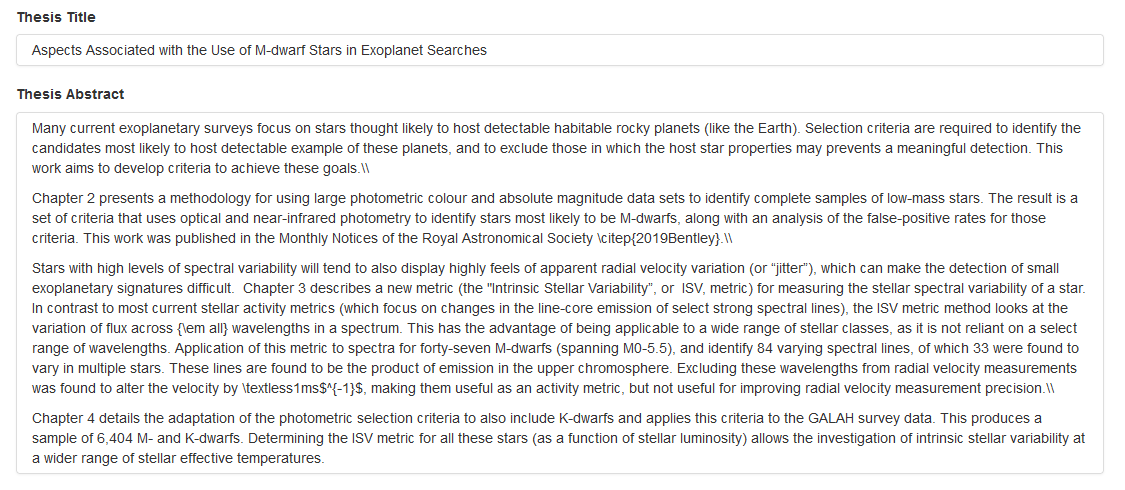
\includegraphics[width=1.3\textwidth]{Abstract.png}
\end{figure}

\section*{2. ORIGINALITY, COPYRIGHT, AND AUTHENTICITY STATEMENTS}
\begin{figure}[H]
    \hspace{-3cm}
    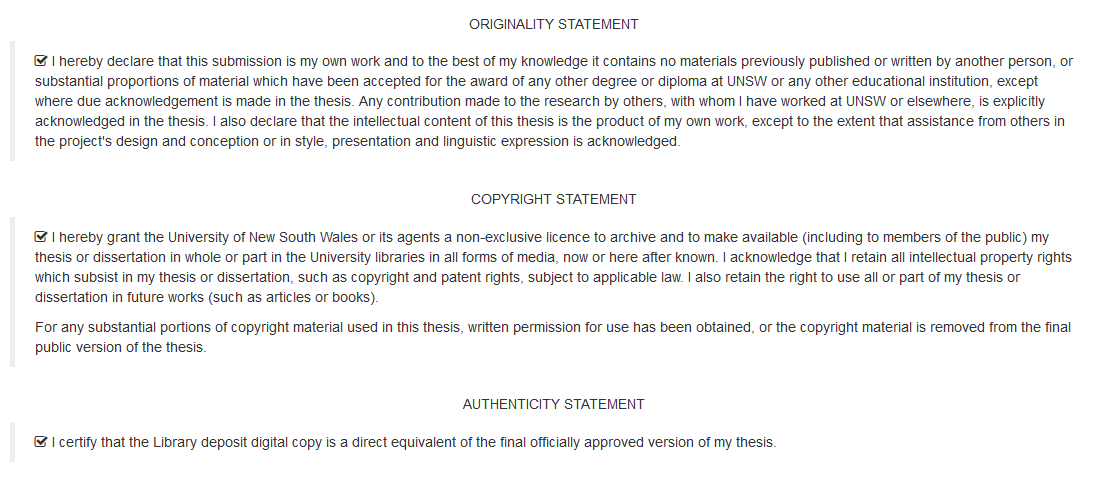
\includegraphics[width=1.3\textwidth]{Origniality.png}
\end{figure}

\section*{3. INCLUSION OF PUBLICATIONS STATEMENT}
\begin{figure}[H]
    \hspace{-2cm}
    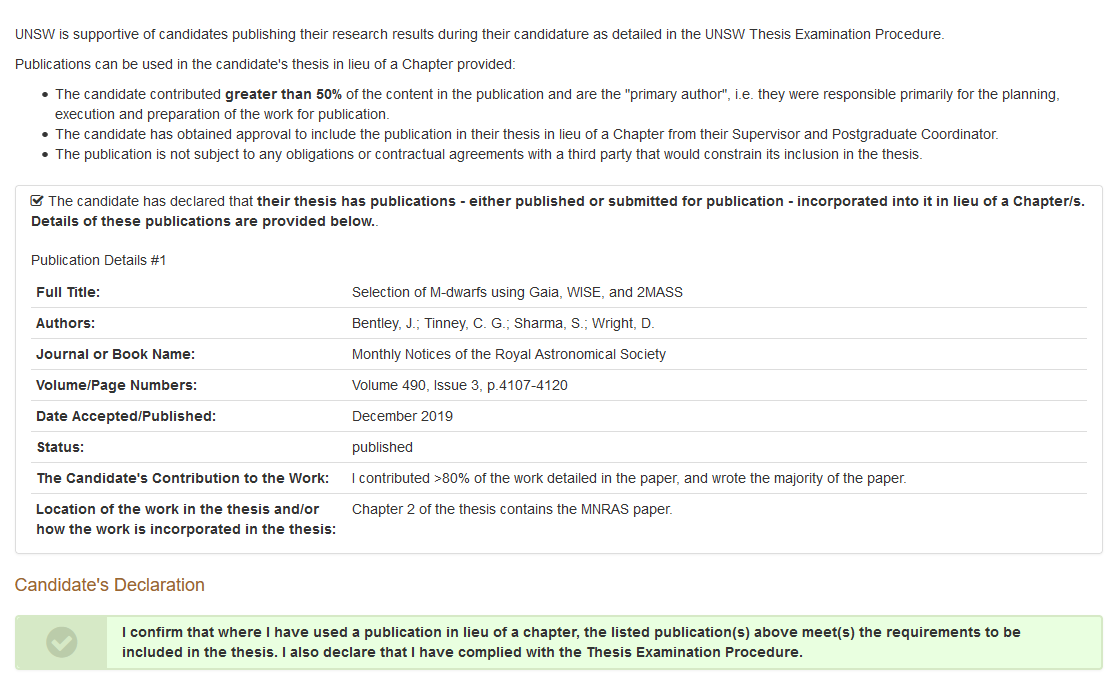
\includegraphics[width=1.4\textwidth]{Publications.png}
\end{figure}
\tableofcontents
\listoffigures
\listoftables
\begin{Large}
\centering
Acknowledgements\\
\end{Large}
\vspace{2cm}
I would like to express my sincere gratitude to the following people who have helped me to get to where I am:\\

First and foremost I am extremely grateful to my supervisors, Professor Chris Tinney and Associate Professor Sarah Martell for sharing their knowledge and steering my research. In particular I would like to thank Professor Tinney for his ability to repair computers at short notice, and Associate Professor Sarah Martell for constantly putting cyan everywhere.\\

Additionally I would like to thank Dr Duncan Wright for initially supervising my work and for spending many hours assisting me with technical issues. Dr Sanjib Sharma also deserves praise for adapting {\em Galaxia} to suit the needs of the photometric selection method of Chapter 2, and Dr Jeffrey Simpson for his assistance in database cross-matching. Professor Jeffrey Linsky for providing me with access to one of his papers. Dr Christoph Bergmann provided multiple opportunities to discuss the issues that arose in the development of the ISV analysis of Chapter 3, and Kirsten Banks for proof reading Chapter 1.\\

Lastly I would like to thank my friends and family. My mother for being an inspiration to persevere, no matter what happens. Tammy and James for distracting me when I needed a break. Lastly Zandra, for just being herself.
\thispagestyle{plain}
\begin{center}
    \Large
    \textbf{Aspects Associated with the Use of M-dwarf Stars in Exoplanet Searches}\\
    \vspace{0.4cm}
    John Bentley\\
    School of Physics, Faculty of Science, UNSW Australia\\
    \vspace{0.9cm}
    \textbf{Abstract}
\end{center}
Many current exoplanetary surveys focus on stars thought likely to host detectable habitable rocky planets (like the Earth). Selection criteria are required to identify the candidates most likely to host detectable examples of these planets, and to exclude those for which the host star properties may prevent a meaningful detection. This work aims to develop criteria to achieve these goals.\\

Chapter 2 presents a methodology for using large photometric colour and absolute magnitude data sets to identify complete samples of low-mass stars. The result is a set of criteria that uses optical and near-infrared photometry to identify stars most likely to be M-dwarfs, along with an analysis of the false-positive rates for those criteria. This work was published in the Monthly Notices of the Royal Astronomical Society \citep{2019Bentley}.\\

Stars with high levels of spectral variability will tend to also display high levels of apparent radial velocity variation (or ``jitter''), which can make the detection of small exoplanetary signatures difficult.  Chapter 3 describes a new metric (``Intrinsic Stellar Variability'', or ISV) for measuring the spectral variability of a star. In contrast to most current stellar activity metrics (which focus on changes in the line-core emission of select strong spectral lines), the ISV metric method looks at the variation of flux across {\em all} wavelengths in a spectrum. This has the advantage of being applicable to a wide range of stellar classes, as it is not limited to a few strong features. Application of this metric to spectra for 46 M-dwarfs (spanning M0-5.5) identified 84 varying spectral lines, of which 37 were found to vary in at least ten of the stars. These lines are found to be the product of emission in the upper chromosphere. Excluding these wavelengths from radial velocity measurements was found to alter the velocity by \textless1ms$^{-1}$. ISV is useful as an activity metric, but it does not dramatically improve radial velocity measurement precision.\\

Chapter 4 details the adaptation of the photometric selection criteria to also include K-dwarfs and applies this selection to the GALAH survey data. This produces a sample of 6,405 M- and K-dwarfs. Determining the ISV metric for all these stars (as a function of stellar luminosity) allows for an investigation of how the strength and measurement uncertainty of the spectroscopic variation detected by the metric change with absolute magnitude. Stellar variability is expected to influence abundance measurements. Comparison of the abundances of quiescent and active stellar lines (identified via the ISV metric) indicate that the ISV metric may be a potential tool for identifying significantly variable spectral lines that would produce discrepant abundance measurements.\\


\pagenumbering{arabic}
\chapter{Background}
\section{Exoplanets}
While we have observed and characterised the planets in our own Solar system for many hundreds of years, the detection of planets orbiting other stars is a relatively new field. The first confirmed exoplanet detection occurred serendipitously, when \citet{1992Wolszczan} observed periodic variations in the timing of the pulses from the pulsar PSR1257+12. Their analysis found that the best explanation for these variations was the presence of two exoplanets with masses 4.3 and 3.9 times the mass of Earth on orbits with semimajor axes 93\% and 119\% of the distance between Mercury and the Sun. Three years later \citet{1995Mayor} found evidence of the first exoplanet orbiting a main sequence star using periodic variations in the radial velocity of the star 51 Pegasi. The exoplanet 51 Pegasi b has a mass 149 times that of Earth and is orbiting at 13\% of the Mercury-Sun distance \citep{2006Butler}.\\ 

Because planets are so much fainter than the stars they orbit, and lie close to those stars on the sky, exoplanetary science almost always uses indirect methods to detect and study these systems. The key properties of an exoplanet that we seek to understand are its mass, composition, and distance from its host star. Exoplanets display a wide range of intrinsic properties such as planetary radius, mass, and atmosphere. While we have used the planets of our Solar system as a template, we cannot be sure that our Solar system is typical. We have found multiple exoplanets with characteristics unlike the planets in our Solar system. For example, the mass of 51 Pegasi b puts it into the Jupiter category, but its orbital radius is 0.0527\,$\pm$\,0.0030 AU, making its surface temperature much hotter than Jupiter itself. Thus 51 Pegasi b became the first known ``hot Jupiter''. Hot Jupiters are more readily detectable to indirect methods than lower-mass planets on longer orbits (see Section\,\ref{secRVPrecision}) and so they formed the majority of discovered exoplanets for a number of years. At first glance this would suggest that close-in gas giants are more common than the ``cold Jupiter'' in our Solar system. However, with the development of exoplanet detection techniques, it has become clear that cold Jupiters are roughly 8 times more common than hot Jupiters \citep{2020Wittenmyer}.\\

In the decades since that first Jupiter-mass planet detection, larger telescopes, higher spectroscopic resolution, improved spectrograph stability, and continued development of data analysis techniques have allowed us to detect smaller and less massive exoplanets. Space-based exoplanet surveys have also played a significant role -- to date, 76\%\footnote{https://exoplanets.nasa.gov/discovery/discoveries-dashboard/} of exoplanets have been detected by space telescopes. Our ultimate goal is to find exoplanets similar to our own planet. Due to our past technological limitations, the fraction of Earth-size exoplanets out of the total number we have detected is relatively low. However, our capabilities are improving, and detection of Earth-sized exoplanets will soon become common.\\

Exoplanet detection requires large volumes of observational data. The probability of detecting exoplanets orbiting any given star is low, while observing time with the most capable telescopes and instruments is limited, so we must optimise by focusing our observations on the stars that are most likely to be hosting the Earth-sized rocky exoplanets we are looking for, and those stars are M-dwarfs.\\

\section{M-dwarfs}
\label{secMdwarfs}
M-dwarfs are the most common type of star in the Galaxy, comprising around 75\% of stars \citep{2007Tarter}. M-dwarfs are the smallest, coolest and least massive stars on the main sequence (Table\,\ref{tabMsub}). Due to the low temperatures of M-dwarf atmospheres, molecules can form that would be destroyed in much hotter stars. Strong absorption features corresponding to titanium oxide (TiO) and vanadium oxide (VO) are observed in optical spectra, while absorption features of carbon monoxide and water are dominant in the near-infrared \citep{2007Tarter,1943Morgan}.\\

\begin{table}[!h]
\centering
\begin{tabular}{| c | c | c | c | c | c | c | c | c | c |}
\hline
SpTy & T & R & Mass & L/100 & M$_{V}$ \\
Dwarf & (K) & (R$_{sun}$) & (M$_{sun}$) & (L$_{sun}$) & (mag) \\
\hline
M0 & 3800 & 0.62 & 0.60 & 7.2 & 9.34 \\
M1 & 3600 & 0.49 & 0.49 & 3.5 & 9.65 \\
M2 & 3400 & 0.44 & 0.44 & 2.3 & 10.12 \\	
M3 & 3250 & 0.39 & 0.36 & 1.5 & 11.15 \\
M4 & 3100 & 0.26 & 0.20 & 0.55 & 12.13 \\	
M5 & 2800 & 0.20 & 0.14 & 0.22 & 16.0 \\
M6 & 2600 & 0.15 & 0.10 & 0.09 & 16.6 \\
M7 & 2500 & 0.12 & ~0.09 & 0.05 & 18.8 \\	
M8 & 2400 & 0.11 & ~0.08 & 0.03 & 19.8 \\
M9 & 2300 & 0.08 & ~0.075 & 0.015 & 17.4 \\
\hline
\end{tabular}
\caption{M-dwarf physical characteristics for each subclass, from \citet{2005Reid}. Note the M4 radius has been altered from 0.36\,R$_{sun}$ to 0.26\,R$_{sun}$, as per \citet{2009Kaltenegger}.}
\label{tabMsub}	
\end{table}

A number of molecular features in M-dwarf spectra vary as a function of temperature and 
luminosity, and have been used as the basis for spectral type classifications that allocate subtypes from warmer (or ``early'') M-dwarfs at M1 to cooler (or ``later'') subtypes at M5-M8. M-dwarf subtype classification was historically complicated by the fact that M-dwarfs emit the majority of their flux in the infrared, and most stellar classification systems had been developed using spectra at optical wavelengths. The most widely adopted spectral classification system currently in use for M-dwarfs was defined by \citet{1991Kirkpatrick}, who based their system on the strengths of TiO and VO absorption bands in the 6300\,-\,9000\,\hbox{\AA} wavelength range. Each individual absorption band tends to grow in strength as we move to cooler stars but then saturate, and so its usefulness as a diagnostic is limited to a certain temperature range. To accommodate this, the \citet{1991Kirkpatrick} classification scheme uses the strength of multiple molecular bands across the wavelength range 6300\,-\,9000 \hbox{\AA} to cover the full range of M-dwarf subtypes. For example, the TiO band at 7050\,\hbox{\AA} can be used for classification of subclasses M0-M5 \citep{2005Reid}, but from M6 onwards the TiO band strength saturates and the classification depends on VO bands. Metal hydrides such as MgH, FeH, and CaH appear weakly in early M-dwarfs and gain strength in later subtypes \citep{2005Reid}. Example spectra from the \citet{1991Kirkpatrick} classification scheme, with important features marked, are shown in Figure~\ref{figMD_sub}.\\

\begin{figure}
\centering
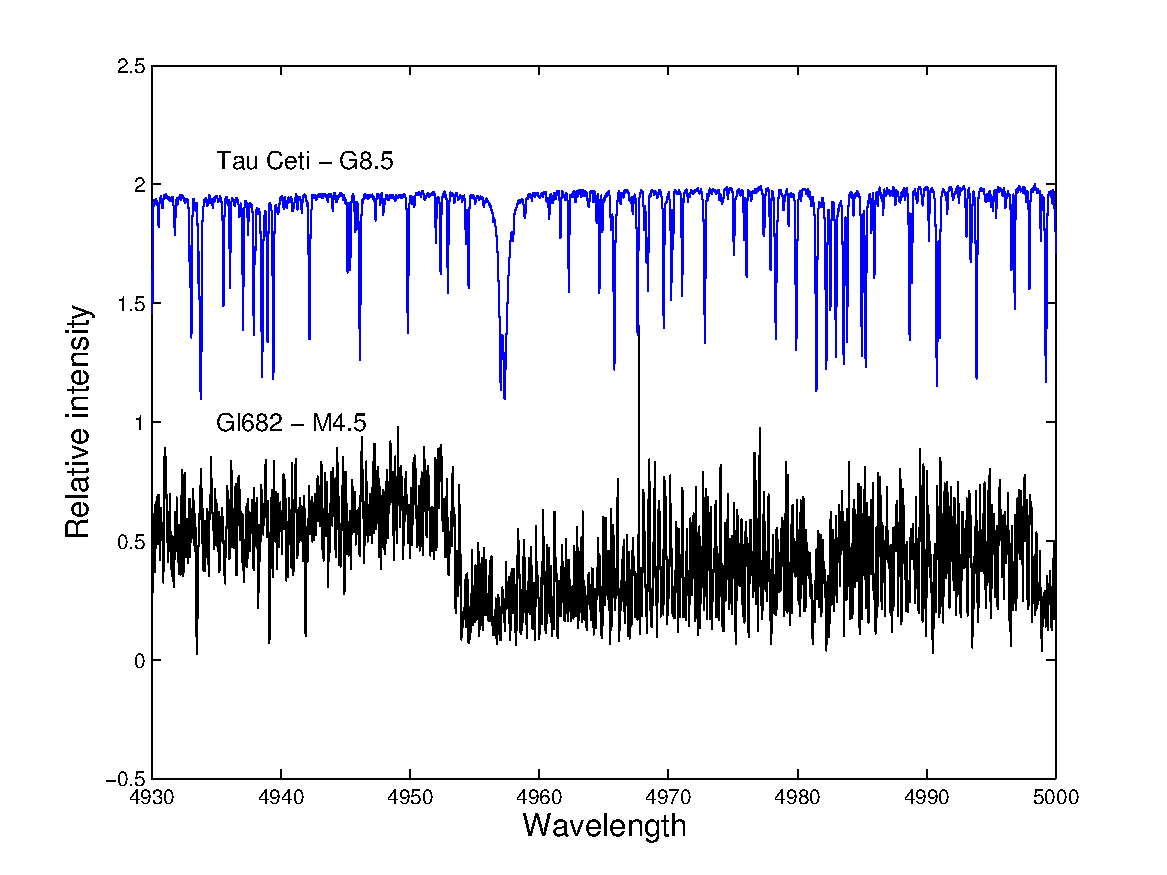
\includegraphics[width=\textwidth]{TauCetiGl682_comparison.pdf}
\caption{Spectra of a G4.5 star, Tau Ceti, and a M8.5 star, Gl682. The spectra have been offset vertically to provide visual clarity. Of note is the molecular bandhead present in the spectra of Gl682 at $\sim$4955\,\hbox{\AA}.}
\label{figSpec}
\end{figure}

Molecular bands like these contain a large number of narrow and closely spaced absorption features, due to the large number of rotational and vibrational energy states available to molecules, and their overall effect on a spectrum is a sharp drop in flux at a particular wavelength and a broad zone of absorption stretching to lower or higher energy. An example of a such a molecular band can be seen in Figure \ref{figSpec}, where the sharp drop of a TiO bandhead is located at $\sim$4955\,\hbox{\AA} and the strength of the absorption decreases toward redder wavelengths. The width of molecular absorption bands can make it difficult to reliably locate the continuum in a spectrum. This complicates spectroscopic analysis, including the measurement of band strength indices and activity (see Section\,\ref{secVarQuant}).\\

\begin{figure}
	\captionsetup{width=.8\textwidth}
	\subfloat[]{\label{figMD_sub_1}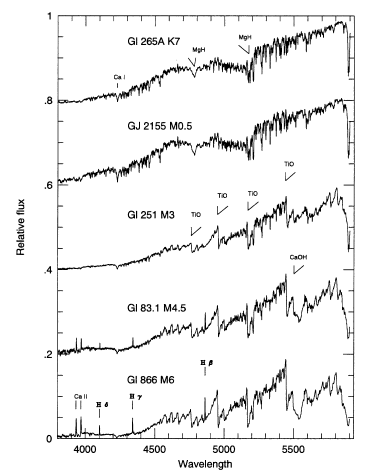
\includegraphics[width=0.52\textwidth]{MD_subclass_1.png}}
    \subfloat[]{\label{figMD_sub_2}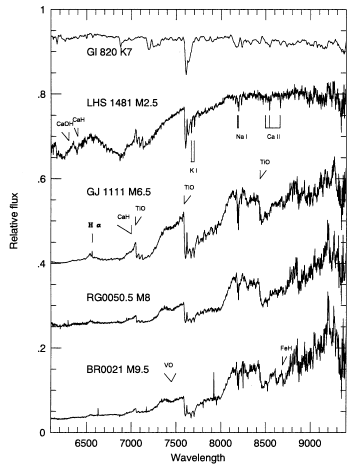
\includegraphics[width=0.5\textwidth]{MD_subclass_2.png}}
    \caption{Spectra of several stars across a range of M-dwarf subclasses and the spectroscopic features used by \citet{1991Kirkpatrick} to classify them. Source: \citet{2005Reid}.}
    \label{figMD_sub}
\end{figure}

\subsection{The habitable zone}
\label{secHab}
Much of current exoplanetary science is motivated by a desire to understand how common potentially habitable planets are in the Universe. One aspect of this is the hunt for observable ``biosignatures'' that could indicate the presence of life. The idea of searching for {\em potentially} habitable exoplanets orbiting in the ``habitable zone'' has become important. The habitable zone of a star is the range of orbital distances at which a rocky exoplanet can retain liquid water at its surface \citep{1993Kasting}. There are multiple parameters that will determine an exoplanet's habitable zone, including its orbital radius, planetary rotation speed, and the mass of the host star. The most significant factor for habitability is the exoplanet's surface temperature, which is primarily dependent on the incident radiation on the exoplanet and therefore on the orbital radius. For a given star system, the location of the habitable zone can vary over time due to the evolution of the star. The habitable zone of the Solar system currently extends from 0.9 to 1.4 AU. Once the Sun ends its hydrogen burning phase, it will evolve into a red giant and the inner boundary of the habitable zone will move outward as the Sun expands, ultimately moving past the Earth. Due to the low luminosity of M-dwarfs, their habitable zones are much closer to the star than for the Sun. Models developed by \citet{2013Kopparapu} predict that a typical M-dwarf habitable zone is 0.2 to 0.8 AU. The fact that the habitable zone for an M-dwarf is quite close to the star makes them important candidates for exoplanet detection, as discussed in Section\,\ref{secTrans}.\\

\section{Exoplanet detection}
\label{secDetectMeth}
Figure\,\ref{figExoHist} shows how the rate of exoplanetary discovery has increased rapidly over time, as the community has continued to develop and improve detection methods. There are a variety of methods that can be used to detect and characterise exoplanets; however, some have been more successful than others. The two methods with the highest yield of planets to date are photometric transits and radial velocity spectroscopy. These two methods allow us to not only detect an exoplanet and determine the parameters of its orbit, but also to estimate its radius (photometric transits) or mass (radial velocity spectroscopy). When both methods can be used together on the same exoplanet, the combined information allows for an estimate of the exoplanet's density and composition.\\

\begin{figure}
    \centering
    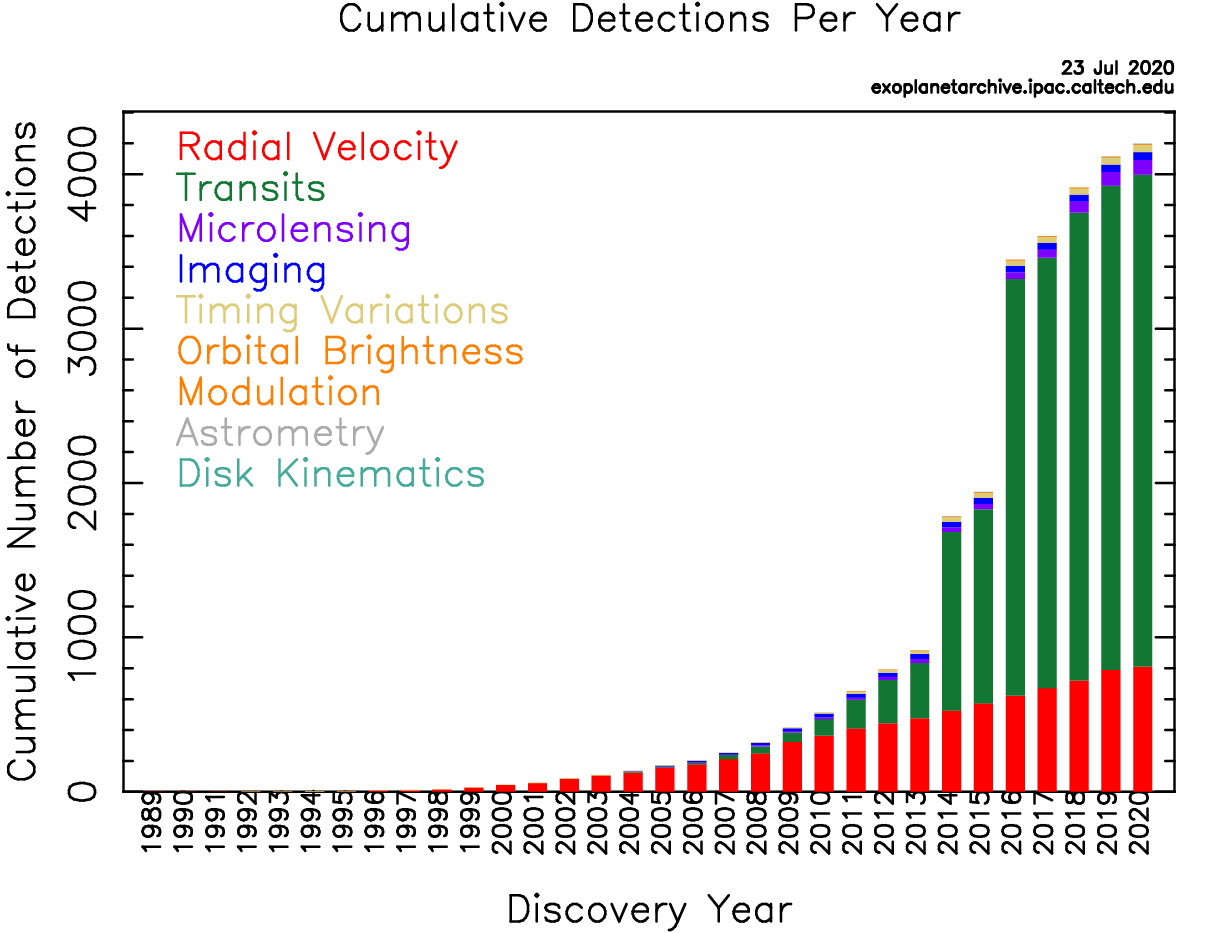
\includegraphics[width=\textwidth]{exo_dischist_cumulative.png}
    \caption{Cumulative histogram of the number of confirmed exoplanets over time. 
    Source: https://exoplanetarchive.ipac.caltech.edu/exoplanetplots/exo\_dischist\_cumulative.png.}
    \label{figExoHist}
\end{figure}

\subsection{Transits}
\label{secTrans}
Transits occur when the path of an exoplanet's orbit aligns with our line of sight to the star. When we observe a transit, the amount of light from the star will change with the position of the exoplanet. Taking Figure\,\ref{figTransit} as an example, when the exoplanet is orbiting outside of the visible disc of the star, the total light we observe is at a maximum. This is the combination of the light from the star and some of the light reflected by the exoplanet. As the exoplanet moves in front of the face of the star, it obscures a small region of the surface of the star, and none of the reflected light is pointing towards Earth. The apparent brightness we observe for the star is at a minimum at this point in the orbit. A smaller secondary dip can be seen when the exoplanet moves behind the star, blocking the reflected light and leaving only the flux directly from the star.\\

\begin{figure}[hbt]
\centering
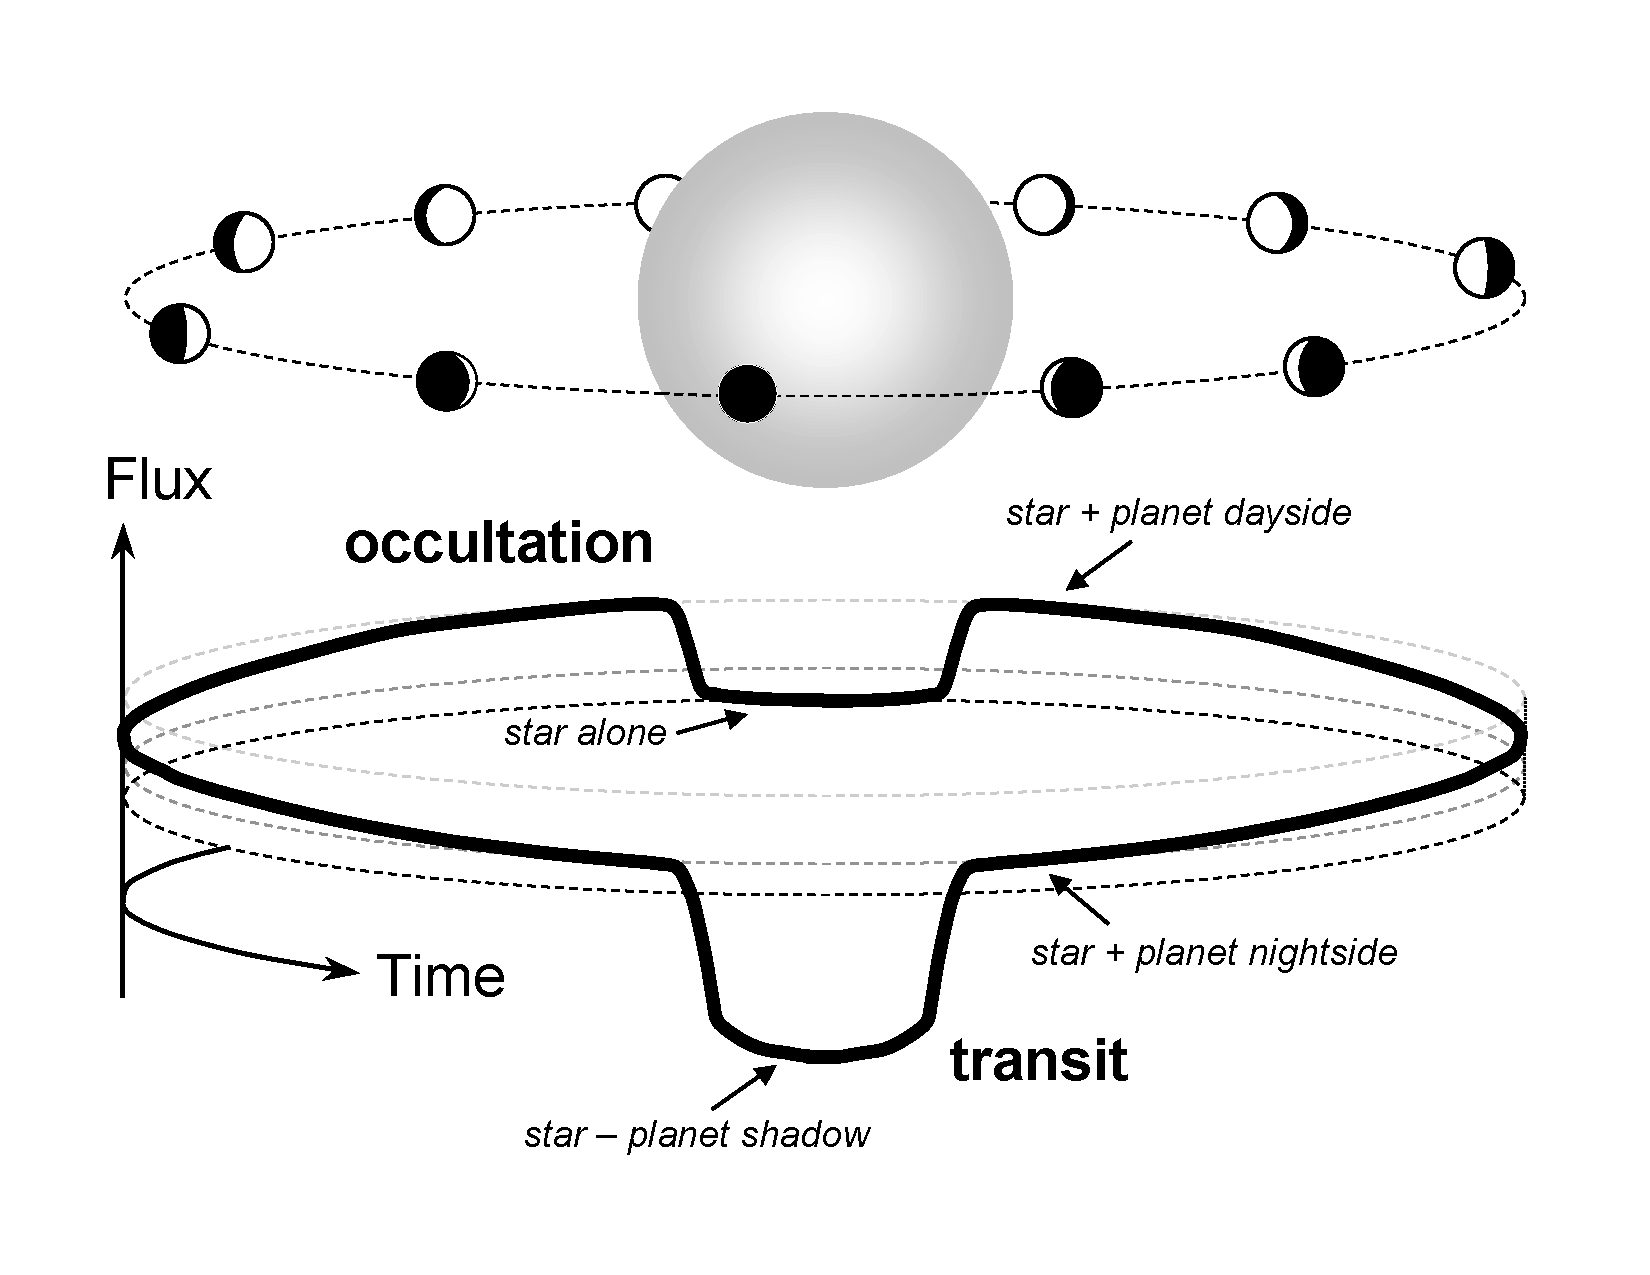
\includegraphics[scale=0.4]{circular_diagram.pdf}
\caption{Diagram showing the effect on the apparent brightness of a star when an exoplanet passes across the visible face of the star. Source: \citet{2010Winn}.}
\label{figTransit}
\end{figure}

We can use this drop in flux to estimate the radius of the exoplanet. Assuming that the stellar disc is uniformly bright, the maximum drop in flux, $\Delta F$, is related to the radii of the exoplanet, $R_p$, and the star, $R_\ast$, through Equation\,\ref{eqFluxDrop}. 

\begin{equation}
\Delta F = \left(\frac{R_p}{R_\ast}\right)^2
\label{eqFluxDrop}
\end{equation}

$\Delta F$ can be determined by a well sampled photometric light curve and $R_\ast$ can be estimated from models of the stellar size as a function of either luminosity (from photometry and distance) or temperature (estimated from photometric colour). In reality the stellar disc is not uniform and limb darkening, where the star is darker at the edges of the disc due to varying optical depth, needs to be taken into account. However, to first order Equation\,\ref{eqFluxDrop} is a reasonable estimate. As an example, if we observed a Jupiter-sized exoplanet transiting a star like the Sun, the drop in flux would be $\sim$1\%. Transit signals in M-dwarfs do not require as much photometric precision as in more massive stars, because the planets are larger relative to the stars, making $\frac{R_p}{R_\ast}$ larger) \citep{2011Lepine}.\\

\begin{figure}
\centering
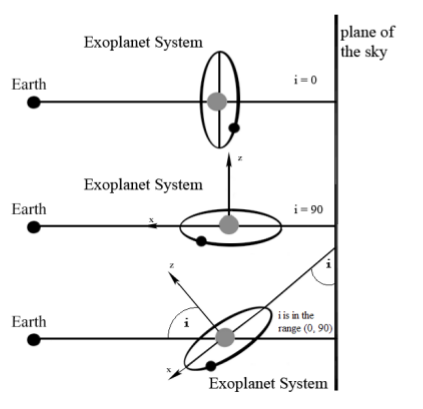
\includegraphics[width=0.7\textwidth]{OrbitalPlane.png}
\caption{Diagram showing the angle representing the orbital inclination of an exoplanet orbiting a star. Source: \citet{1998Zeilik}.}
\label{figOrbit}
\end{figure}

Transits can only be seen if the inclination of the system's orbital plane is close to edge-on ($i \approx 90^\circ$; see Figure\,\ref{figOrbit}). The actual distribution of orbital inclinations will range from $0^\circ$ to $90^\circ$. Assuming randomly distributed orbital orientations and circular orbits, the probability that a given system will have an observable exoplanet transit can be calculated from Equation \ref{eqTransProb}, where $a$ is the semi-major axis of the exoplanet's orbit.\\

\begin{equation}
P_{transit} = \frac{R_\ast + R_p}{a}
\label{eqTransProb}
\end{equation}

For example, if we were observing a star like the Sun, and it had a planet like the Earth, then the probability that the alignment would allow us to see transits would be 0.47\%\citep{2003Borucki}, meaning that we would need to observe approximately 200 of these stars to find one that would transit. Systems containing a large star and/or exoplanet, and those where the exoplanet's orbital radius is small, will have the greatest probability of transiting. Exoplanets orbiting close to their host star, such as habitable zone exoplanets around M-dwarfs, are more likely to have an orbit that allows for the detection of a transit than those on larger orbits. For example, an Earth-sized exoplanet orbiting within the habitable zone of an M7 star (a = 0.35 AU) has a transit probability of $\sim$2.0\%, which is almost four times the transit probability for the same planet orbiting in the habitable zone of the Sun. To accommodate this low geometric transit probability, transit surveys tend to observe large areas of the sky, as their chances of observing a transit increase proportionally with the number of stars observed. The closeness of the habitable zone in M-dwarfs is an advantage to exoplanet detection because of the higher probability of a planet transiting. Planets with smaller orbital radii will have short orbital periods, which allows photometry of multiple orbits to be obtained over a shorter period of time, returning light curves that are well sampled across orbital phase and allowing precise determination of orbital period and transit depth.\\

\subsubsection{Transit surveys}
\label{secTransitSurveys}
There have been a number of ground- and space-based photometric surveys with a focus on exoplanetary transits. The surveys that are of particular importance to this thesis are Kepler, TESS, and the MEarth project. These large survey projects provide photometry in the optical (Kepler) and near-infrared (TESS), which are the wavelengths where M-dwarfs emit most of their flux.\\

The Kepler mission\,\citep{2010Koch} was a spaced-based photometric survey that continuously observed around 150,000 stars across a 115 square degree field of view in an area of the sky around the Cygnus and Lyra constellations. The main aim of continuous photometry of so many stars was the detection of Earth-like exoplanets orbiting in the habitable zone of their star, and the data were also of significant use for studies on asteroseismology \citep{2009Stello} and eclipsing binaries \citep{2006Gimenez}. The survey was initially planned for 3.5 years, starting in 2009, and it was extended to 2016 due to greater than expected stellar variability, which reduced the statistical significance of a transit and resulted in far fewer confirmed transits by Earth-sized exoplanets in the habitable zone than predicted. The Kepler survey team initially estimated they would need three transits per star to get a statistically significant 4\,$\sigma$ light-curve signal-to-noise ratio \citep{2011Gilliland}. However, the variability added noise to the photometric measurements, making additional observations necessary to meet the data quality goals. This extension was interrupted by a technical fault in 2013, when two of the four onboard reaction wheels providing fine pointing control failed. Although Kepler was unable to continue with its initial mission, a ``K2'' mission was developed \citep{2014Howell} in which the spacecraft would observe fields along the ecliptic for 75 days per field. This choice of observing fields allowed the pointing to remain highly stable with only two reaction wheels. The new science goals included observing the transits of nearby low-mass stars (like M-dwarfs), bright stars (V\,\textless\,12), and stars within open clusters, as well as observing star forming regions, type Ia supernovae, and microlensing events. Overall Kepler observed 530,506 stars and detected transits of 2,662 exoplanets across both the original and K2 surveys. An important achievement of Kepler was the discovery of Kepler-22b, the first exoplanet orbiting a Sun-like star in the habitable zone. The planet was found to have a radius of 2.4\,R$_\oplus$ and a mass less than 53\,M$_\oplus$ \citep{2013Kipping}.\\

The Transiting Exoplanet Space Satellite \citep[TESS;][]{2009Ricker} was designed as a followup to the work of the Kepler spacecraft, and it is the current leading source of transiting exoplanet detections, especially around M-dwarfs. Its focus is high quality, high-cadence, wide-field photometry of around 500,000 stars in the Solar neighbourhood, particularly F5-M5 main sequence dwarfs, looking for transiting exoplanets. TESS observes the entire sky, broken into 26 panels of 24 by 96 degrees, with each panel observed for around 27 days. Areas near the ecliptic poles are observed as part of multiple panels, creating a longer time series of data in those regions of sky. Specific targeted stars are observed every 2 minutes, while an image of the full panel is recorded every 30 minutes. Between the observation length and the cadence, TESS transit data focuses on planetary orbits of around 10 days for most stars, and up to 40 or more days for stars near the ecliptic poles.\\

The MEarth project \citep{2008Nutzman} was designed to observe 2,000 nearby (d\,\textless\,33\,pc) M-dwarfs, visible in the northern hemisphere, looking for planetary transits. It is located at the Fred Lawrence Whipple observatory, and uses 8 automated 40cm telescopes. Unlike many current transit surveys, MEarth observes each star sequentially, rather than simultaneously. One of the first major discoveries of the project was GJ1214b \citep{2009Charbonneau}, a 6.55\,M$\oplus$, 2.68\,R$\oplus$ super-Earth orbiting around a star only 13\,pc from Earth. In 2015 an Earth-sized planet was found by the team, orbiting GJ1132 with a radius of 1.2\,R$\oplus$ \citep{2015BertaThompson}. With further analysis, the team determined that GJ1132b had a similar density to Earth, but was orbiting too close to its host star that, while still expected to contain an atmosphere, would not be habitable. Another discovery was a 1.4\,R$\oplus$ planet around LHS1140 \citep{2017Dittmann}. LHS1140b is significant as analysis predicts that the environmental conditions would allow for liquid water to be present on the surface. A second array of MEarth telescopes was built at the Cerro Tololo observatory in Chile \citep{2014BertaThompson}.

\subsection{Radial velocity spectroscopy}
\label{secRVanalysis}
In a planetary system, the star and all the planets orbit their common centre of mass, or barycentre. Figure\,\ref{figOrbit} illustrates this arrangement, and is exaggerated to clearly display that both the star and the planet are moving. Because the star in a real planetary system is much more massive than the planet, the barycentre will be quite close to the centre of the star. 
The more massive the planet is, the further the barycentre will shift away from the centre of mass of the star. As a result, the motion of the star will be small, and so will its velocity, and that velocity signal carries information about the planet's mass and orbit. As an example, the Earth produces a 0.09~ms$^{-1}$ oscillation in the velocity of the Sun with a period of one year, while Jupiter induces a 12.7~ms$^{-1}$ signal with a period of 11.862 years. We can measure the radial velocity of a star from its spectrum by comparing the observed wavelength of a selected spectral line, $\lambda_{obs}$, to its rest wavelength $\lambda_{rest}$. The radial velocity $v_{R}$ is then given by Equation\,\ref{eqRV}, where $c$ is the speed of light.\\

\begin{equation}
    v_{R} = \frac{\lambda_{obs}-\lambda_{rest}}{\lambda_{rest}}c
    \label{eqRV}
\end{equation}

We can improve the precision of this measurement by measuring the shift for many spectral lines simultaneously and combining the results. One common way to achieve this is to cross-correlate the spectrum with a real or synthetic template spectrum with a known radial velocity. A real template spectrum would be taken from observations of a star with the same class as the target star and would often be used in conjunction with a line mask that will restrict the cross-correlation to only the strongest of spectral lines in the spectrum. Synthetic spectra can be  produced by models of a star's atmosphere. One example of this is the PHOENIX code \citep{Phoenix}, which can produce synthetic spectra of stars for a range of temperatures and surface gravities. As long as the star in question and the template star have reasonably similar stellar parameters, the resulting Cross Correlation Function (CCF) is maximised or minimised at the velocity shift required to align the observed spectrum to the template spectrum. Figure\,\ref{figCCF} shows the CCFs for two stars, with the resulting radial velocities marked with vertical dashed lines \citep{2020Morris}. \\

\label{secRV}
\begin{figure}
    \centering
    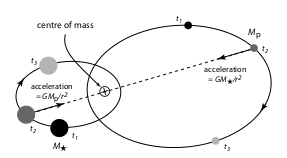
\includegraphics[width=0.8\textwidth]{Barycentre.png}
    \caption{Diagram of a star and a planet orbiting the system's barycentre (labelled as ``centre of mass'' in the diagram). Source: \cite{2011Perryman}.}
    \label{figBary}
\end{figure}

\begin{figure}
    \centering
    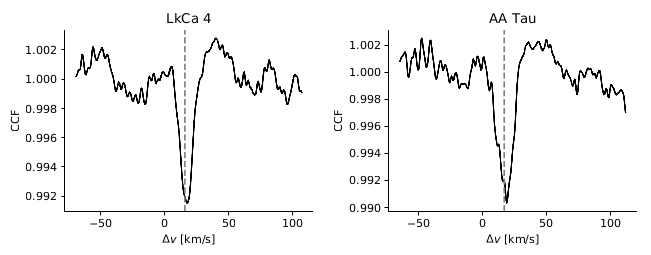
\includegraphics[width=0.8\textwidth]{CCF.png}
    \caption{CCFs for the stars LkCa 4 and AA Tau. The vertical dashed lines mark the radial velocity obtained from the cross-correlation. Source: \citet{2020Morris}.}
    \label{figCCF}
\end{figure}

A radial velocity monitoring campaign for a given star will produce a series of radial velocities. These campaigns are ideally well sampled across multiple planetary orbits to avoid problems with aliasing. We can search for any periodic changes in the radial velocity using least-squares analysis to produce a Lomb-Scargle periodogram \citep{1976Lomb,1982Scargle}. False Alarm Probabilities (FAP) can be calculated to determine how likely it is that a periodogram peak of a given strength was produced solely by noise in the data. The horizontal dotted line in Figure\,\ref{figHD85512Power} represents a 10\% FAP, meaning that noise will produce a peak of that magnitude 10\% of the time. The dashed line is the FAP for 1\%. Assuming an exoplanet's influence on the radial velocity is strong enough, its signal will be prominent in the periodogram and greater than the chosen FAP.\\

\begin{figure}
    \centering
    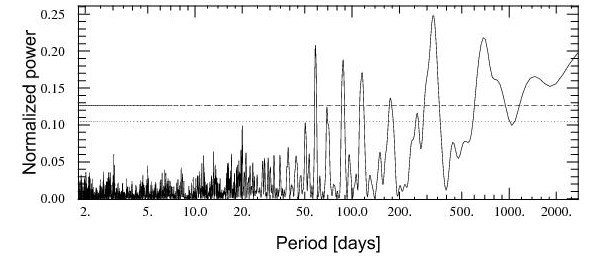
\includegraphics[width=0.8\textwidth]{HD85512_Power.jpg}
    \caption{A periodogram produced from the radial velocities of HD85512. Dashed and dotted horizontal lines indicate FAP of 1\% and 10\% respectively. Source: \citet{2011Pepe}.}
    \label{figHD85512Power}
\end{figure}

For example, \citet{2011Pepe} found several significant peaks in the radial velocity periodogram of HD85512 (Figure\,\ref{figHD85512Power}). A Keplerian model of the radial velocities from a star and planet system was generated from initial estimates of the parameters of the exoplanet (orbital period, eccentricity, planetary mass). The period was selected as each of the peaks of significance in the periodogram and the remaining parameters were varied until the residuals in the radial velocity between the data and the model were minimised. After all the significant peaks were investigated, the influence of an exoplanet with a period of 58.4 days was found in the data (see Figure\,\ref{figHD85512Phased}). The radial velocity signal produced by that planet was removed and a new periodogram, Figure\,\ref{figHD85512Residual}, was produced. In the case of multiple exoplanets, once the first exoplanet is found, its signal is removed from the data, the periodogram is regenerated from the new data, and the process is repeated to see if there are significant and periodic signals remaining in the data. In the HD85512 system, there were no peaks of significance (i.e. above the 1\% and 10\% FAP values) in the periodogram of the residuals, and \citet{2011Pepe} concluded that there were no more planets to be found. Each potential planetary signal needs to be tested against variability measurements to confirm that the signal is not due to a changing stellar environment. Variability is discussed in Sections\,\ref{secVariability}-\ref{secVarQuant} and the impact of variability on HD85512 is detailed in Section\,\ref{secVarApp}.\\

\begin{figure}
    \centering
    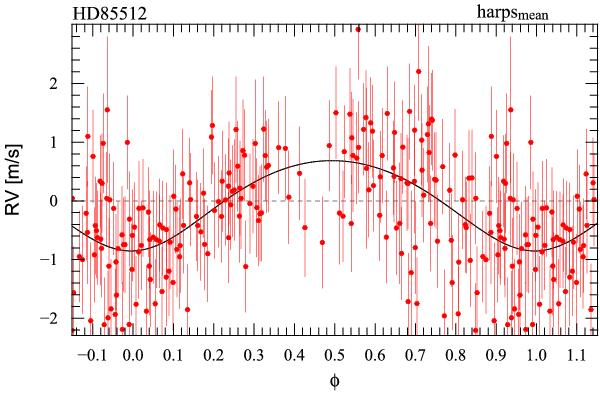
\includegraphics[width=0.8\textwidth]{HD85512_Phased.jpg}
    \caption{Radial velocity for the exoplanet with a orbital period of 58.4 days highlighted in Figure~\ref{figHD85512Periodogram}, as a function of orbital phase $\phi$. The semi-amplitude of the radial velocity variation $K$ is the amplitude of the sinusoid. Source: \citet{2011Pepe}}
    \label{figHD85512Phased}
\end{figure}

\begin{figure}
    \centering
    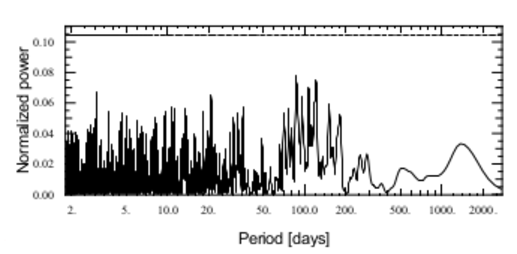
\includegraphics[width=0.8\textwidth]{HD85512_residuals.pdf}
    \caption{Periodogram of the HD85512 radial velocities once the influence of a 58.4 day planet was removed. Source: \citet{2011Pepe}}
    \label{figHD85512Residual}
\end{figure}

Once we know an exoplanet exists, we can determine its mass using the parameters derived from the best-fit model. In Equation \ref{eqRVMass}, $m_p$ is the mass of the exoplanet, $K$ is the semi-amplitude of the radial velocity variation, $G$ is the gravitational constant, $e$ is the orbital eccentricity, $i$ is the orbital inclination (see Figure \ref{figOrbit}), $m_\ast$ is the mass of the star and $a$ is the semi-major axis. The only value we cannot derive from this method is the orbital inclination, $i$. As such, we cannot derive the exact mass of the exoplanet, $m_{p}$, but instead can only determine its minimum mass, $m_{p}\sin(i)$.\\

\begin{equation}
K = \sqrt{\frac{G}{1-e^2}} m_p sin(i) (m_\ast + m_p)^{-1/2} a^{-1/2}
\label{eqRVMass}
\end{equation}

\subsubsection{The influence of spectroscopic precision on radial velocity}
\label{secRVPrecision}
This method has several limitations. First, the radial velocity values we measure are strongly dependent on orbital inclination. We would be unable to detect the movement of stars with orbital inclinations of $0^{\circ}$ (top panel in Figure\,\ref{figOrbit}) and therefore unable to detect the presence of exoplanets by this method. Second, the semi-amplitude of the radial velocity variation, $K$, is dependent on the semi-major axis of the exoplanet's orbit and its mass, in the sense that more massive planets and shorter-period orbits produce larger radial velocity signals. This greater detectability is why hot Jupiters dominated the early days of exoplanet detection. Third, the shape of each spectral line controls how precisely its centroid can be calculated, and therefore how precisely the radial velocity can be calculated. Ideally a spectral line would be narrow, which would allow the centroid of the line to be more accurately determined. There are multiple influences that can broaden a spectral line, and the most influential is the rotation of the star (rotational broadening). \citet{2010Lovis} showed that by assuming a Gaussian profile for a spectral line, the uncertainty $\sigma_{\lambda}$ in the centroid would be proportional to the Full-Width Half-Maximum of the line ($FWHM$) as $\sigma_\lambda \propto FWHM^{\frac{3}{2}}$. M-dwarfs tend to have lower rotational velocities \citep{2005Reid}, so rotational broadening is minimal and the $FWHM$ of a line will be small. \citet{2009Jenkins} studied the rotational velocities of 56 M-dwarfs and found most to be below 10 kms$^{-1}$. A fourth consideration is the number of spectral lines in the observed spectrum, since measuring radial velocity from multiple lines simultaneously leads to a more precise result. The molecular absorption features in the spectra of M-dwarfs create rich forests of lines that are very useful for radial velocity measurement.\\

Perhaps the most important consideration for radial velocity exoplanet detection is velocity precision, which sets a lower mass limit for exoplanet detection. For a confident exoplanet detection, the radial velocity variation amplitude, $K$, needs to be sufficiently larger than the uncertainty associated with each velocity measurement, $\sigma v_{R}$. When the velocity uncertainties are smaller, lower-mass planets are more detectable. The current generation of spectrographs achieve velocity precision of $\sim \pm$1\,ms$^{-1}$, which allows for the detection of small, low-mass, rocky exoplanets in potentially habitable orbits (i.e. exoplanets similar to Earth), which are the priority for current and future exoplanet searches. In the first decade or so of exoplanetary discovery, the best available radial velocity precision was in the $\pm$3-20~ms$^{-1}$ range, permitting the discovery of Jupiter-mass planets on short-period orbits with amplitudes of $\pm$10-100~ms$^{-1}$. Table 2.2 of \citet{2011Perryman} presents a summary of the level of precision achieved by spectrographs in the early years of exoplanet detections. Data for the discovery of 51 Pegasi b \citep{1995Mayor} were acquired with the ELODIE spectrograph \citep{1996Baranne} on the 1.93m telescope at Observatoire de Haute-Provence. The data had a resolution of 42,000, allowing a radial velocity precision of $\pm$\,13\,ms$^{-1}$. The HARPS spectrograph on the 3.6m telescope at La Silla Observatory is a major facility for exoplanet detection. Its maximum spectral resolution is 115,000, which permits a radial velocity precision of $\pm$0.97\,ms$^{-1}$.\\

One of the most important factors in achieving high radial velocity precision is spectrograph stability. When we are trying to measure very small changes in the position of light in the spectrograph that have astrophysical origins, small changes caused by vibrations or changes in atmospheric conditions become significant. For example, with the HARPS spectrograph, the HARPS team identified that the ambient changes in pressure would produce a radial velocity ``drift'' of 100 ms$^{-1}$ per mbar \citep{HARPS}, which is large relative to the radial velocity signal of exoplanets. One mitigation strategy that is used in newer spectrographs is to eliminate moving parts and put the spectrograph into a pressurised tank to control the pressure and temperature. For HARPS, the spectrograph is in an evacuated tank with a pressure below 0.01 mbar. The tank is then air conditioned to ensure that the temperature is maintained at 17\,$\pm$\,0.01$^{\circ}$ C. These measures reduce the radial velocity drift to \textless1 ms$^{-1}$ per day \citealt{2003Mayor}.\\

However, we cannot stabilise our spectrographs completely, and so we also need to measure and correct for these changes. A wavelength calibration, such as Th-Ar hollow cathode lamps \citep{2007Murphy} or a laser frequency comb \citep{1999Reichert}, will produce a spectrum of emission lines that can track the changes in how the spectrograph maps wavelength onto detector position. For most astronomical observations it is sufficient to take wavelength calibration data at the start and end of a night. However, for measurements like radial velocity exoplanet work that require extreme precision, it is necessary to track the wavelength calibration from observation to observation. Light from the calibration lamp or the laser comb is passed through the spectrograph along with the light from the science target, allowing the identification and correction of instrument-based wavelength shifts, making the radial velocity measurement more precise.\\

\subsection{Stellar variability}
\label{secVariability}
While stars are, overall, in hydrostatic equilibrium, they have a non-uniform surface and can rotate at significant velocities that vary with latitude. Their atmospheres are dynamic environments, and there are a number of short-timescale processes that affect the light we receive from them. Rotation, convection, oscillations, temperature variations across the surface, magnetic activity cycles, and other small-scale processes all contribute to an overall ``jitter'' in the radial velocity we measure from a spectrum. Instrumental precision can be improved, but the intrinsic velocity stability of a star is out of our control. The jitter seen in active stars can be large enough that it can be a significant obstacle to our ability to confidently identify the radial velocity signatures of exoplanets. While massive exoplanets can produce a radial velocity variation amplitude large enough to be easily distinguished from the jitter, less massive exoplanets produce radial velocity variations on a similar scale to the jitter, making it harder to confidently identify them.\\

\subsubsection{Stellar atmospheres and magnetic fields}
\label{secStelAtmos}
\begin{figure}
    \centering
    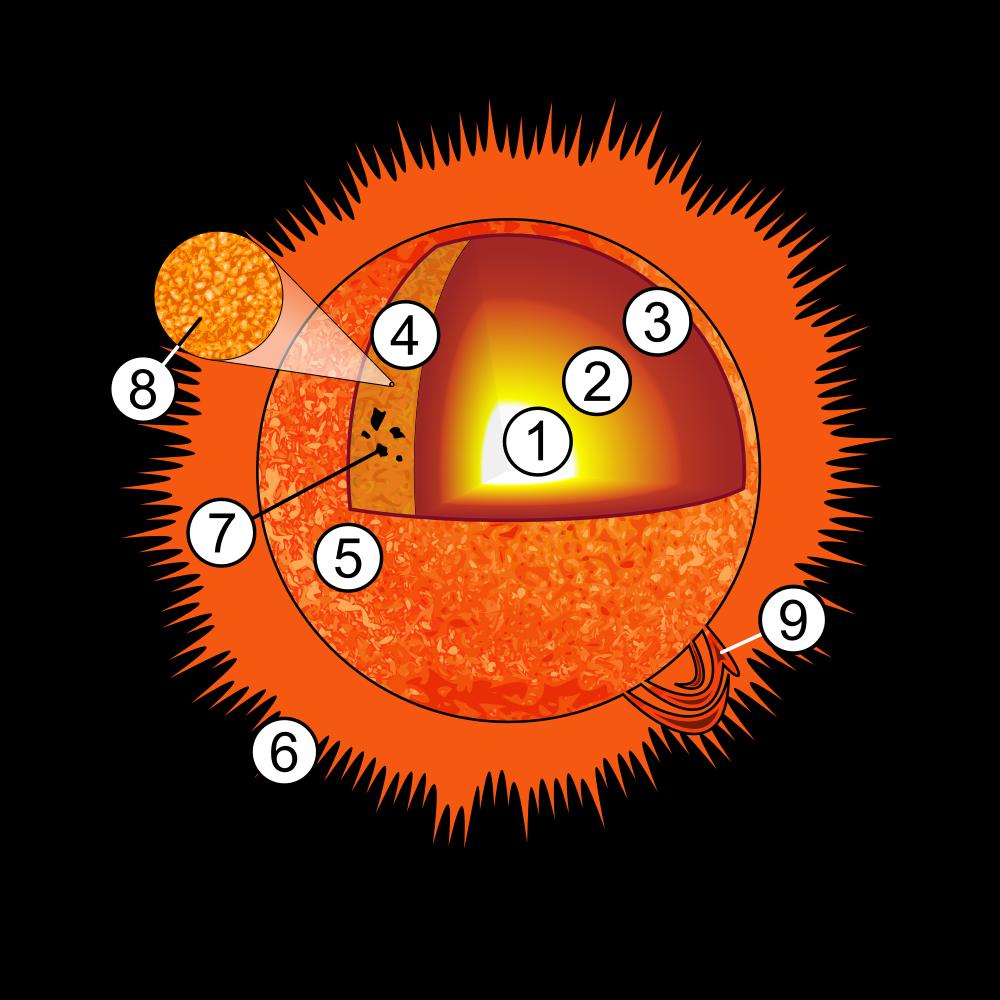
\includegraphics[width=0.6\textwidth]{Sun_diagram.png}
    \caption{Schematic diagram showing the structure of a Sun-like star. The numbered components are:  1. Core, 2. Radiative zone, 3. Convective zone, 4. Photosphere, 5. Chromosphere, 6. Corona, 7. Sunspot, 8. Granules, 9. Prominence. Source: Pbroks13 https://commons.wikimedia.org/wiki/File:Sun\_diagram.svg}
    \label{figStarLayer}
\end{figure}

To understand the astrophysical sources of jitter and their effect on radial velocity measurement, we must consider the structure of the regions that make up the star. Generally, a star has two distinct regions, an opaque interior that produces and transports energy, and a transparent atmosphere that emits the light we see from the star. However, these two regions can then be broken up into additional layers. Figure\,\ref{figStarLayer} labels six layers of a star and three features produced due to stellar magnetic activity. This subsection will discuss the layers of a star, while the following subsection will talk about the stellar activity features.\\

The innermost region of a star is a densely packed region of hot plasma called the core. It is the site of fusion reactions that provide pressure to stabilise the star against gravitational contraction. Outside the core are regions of reduced temperature and density that transport the energy produced by the core to the surface of the star. The structure of these regions, and the methods by which the energy is transported, depend on the mass of the star and the temperature gradient. Energy travelling through a radiative zone is transported as radiation, being absorbed and re-emitted by particles. In a convective zone energy is transported by radiation and mass motion, with hot plasma rising, releasing energy, and sinking back to the base of the convective zone. This cycle produces convective cells, illustrated in Figure\,\ref{figEnergyTrans} as the ellipses in the top layer. Stars more massive than $\approx 2 M_{\odot}$ have convective interiors and radiative exteriors, Sun-like stars have radiative interiors and convective exteriors, and stars with masses \textless0.3\,M$_\odot$ are fully convective and do not have a radiative zone at all. This includes M-dwarfs with types M3.5 and later \citep{2008West}. The details of which regions in a star are stable against convection depend on the opacity and the temperature gradient, with convection only required when the radiation field is not able to transport energy outward as quickly as it is being produced in the core.\\

\begin{figure}
    \centering
    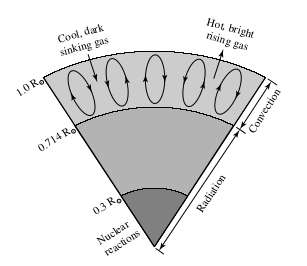
\includegraphics[width=0.6\textwidth]{Convection.png}
    \caption{A schematic diagram of the interior of a Sun-like star. The core produces energy through nuclear fusion, which is then radiated out in the radiative zone. Lastly cells of plasma move in a cycle to transport the energy to the top of the convective zone via convection and convection. Source: \citet{2006Carroll}}
    \label{figEnergyTrans}
\end{figure}

Outside the stellar interior, the first layer of the stellar atmosphere is the photosphere. The photosphere is similar to the convective zone in that there is convective motion present, but is cooler, less dense and is sufficiently transparent for light to have a greater chance of leaving the star and being observed, than of being absorbed. Light moves through the layers of the star in a random walk process, with a mean free path that is dependent on the local density and opacity. The probability of a photon being absorbed and re-emitted is quantified in the optical depth $\tau$, and it is dependent on wavelength and the local sources of opacity. The photosphere of a star is the last scattering surface for photons, which is the depth at which $\tau=2/3$. Since $\tau$ is dependent on wavelength, the depth of the photosphere will vary depending on the wavelength being observed and therefore different spectral features sample the physical conditions at different depths in the star.\\

While the temperature in the stellar interior falls with increasing radius (Figure\,\ref{figSunTempInner}), the layers outward of the photosphere are not so straightforward. The chromosphere is a sparse region situated above the photosphere that opposes the trend of decreasing temperature with increasing radius. The temperature initially decreases in the lower levels of the chromosphere, but then switches and starts to rise, reaching tens of thousands of K at the top (Figure\,\ref{figSunTempOuter}). The reasons for this temperature inversion are complex, and beyond the scope of this work, but essentially it is driven by the presence of magnetic fields in the star \citep{2004Goodman}. Due to this temperature inversion, some elements will produce an absorption line in the cooler regions (the photosphere and lower chromosphere) but also produce an emission line in the upper chromosphere, where the temperature is higher. In particular, the emission from the H$\alpha$ line at 6562.8\,\AA\;and the Calcium H \& K lines at 3968.47\,\AA\;and 3933.66\,\AA\;are quite significant. The outermost layer of a star is the corona. This region extends millions of kilometres into space, and has a temperature of up to 1\,x\,10$^{6}$ K, hot enough to ionise both hydrogen and helium, producing an emission spectrum.\\

\begin{figure}
    \captionsetup{width=.8\textwidth}
    \hspace{-1.5cm}
    \subfloat[]{\label{figSunTempInner}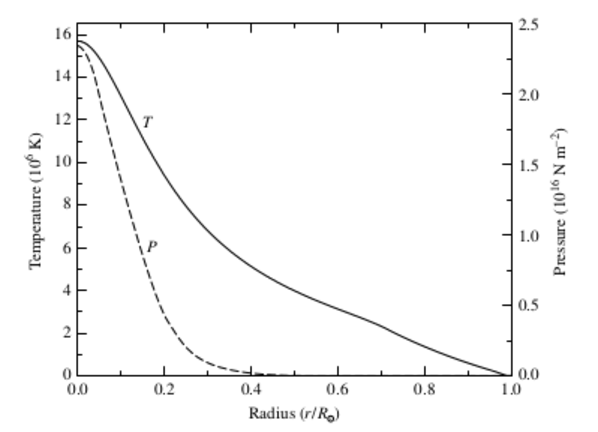
\includegraphics[width=0.6\textwidth]{SunTempInner.pdf}}
    \subfloat[]{\label{figSunTempOuter}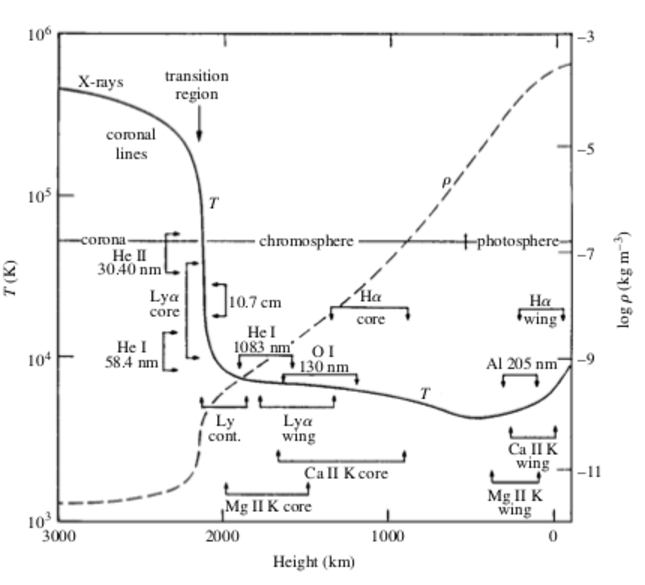
\includegraphics[width=0.6\textwidth]{SunTempOuter.pdf}}
    \caption{Plots of temperature of the interior (left) and atmosphere (right) of the Sun as a function of radius. Source: \citet{2006Carroll}.}
    \label{figSunTemp}
\end{figure}

Threaded through these layers of plasma is a magnetic field formed from stellar rotation and convection within the star, producing a magnetic dynamo. First proposed by \citet{1961Babcock}, dynamo theory states that the motion of charged particles in a star (i.e. the plasma) would induce an electrical current which would in turn induce a magnetic field. Differential rotation of the star will distort the star's magnetic field, twisting the magnetic field lines (shown in panel \textit{b} of Figure\,\ref{figDynamo}), and the interaction of the field lines with the plasma in the star transfers energy from the magnetic field into the stellar atmosphere, heating the chromosphere and producing the stellar activity features discussed in Section\,\ref{secActivity}.\\

In stars with M\,\textgreater\,0.3\,M$_{sun}$, the contrast between the rotation of the interior and the convective zone (solid-body and differential, respectively) produces a region of extreme shear called the tachocline, which will twist the distribution of the magnetic fields across the surface of the star, driving the magnetic dynamo. Stars with M\,\textless\,0.3\,M$_{sun}$ (mid to late M-dwarfs) are fully convective and do not contain a tachocline. The magnetic dynamo of these stars is entirely driven by the differential motion of the convective zone. This will produce significantly stronger magnetic fields than seen in heavier stars, typically 2-5\,kG for active stars \citep{2021Kochukhov}. For comparison, the Sun has a magnetic field of around 1\,G. 

\begin{figure}
    \centering
    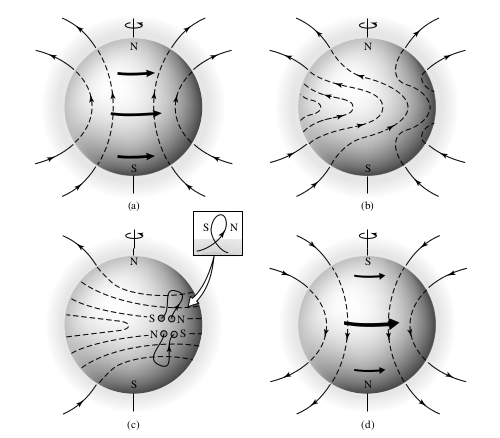
\includegraphics[width=0.8\textwidth]{Dynamo.png}
    \caption{A diagram showing the evolution of a stellar magnetic field. Panel \textit{a} portrays the magnetic field in its initial state, spanning from one pole to the other (poloidal). In panel \textit{b} we see that faster rotation at the equator relative to the poles stretches the field lines across in latitude and the field becomes toroidal. Turbulence from convection will twist the magnetic field into loops that will break through the surface of the photosphere and produce starspots (panel \textit{c}). Eventually the poloidal field will be re-established but with the poles reversed, as seen in panel \textit{d}. Source: \citet{2006Carroll}.}
    \label{figDynamo}
\end{figure}

The magnetic field will go through a cycle of changing magnetic field distribution, from a perfectly longitudinal field from pole to pole (poloidal) to a distorted and predominantly latitudinal field (toroidal) and back again. In the Sun this cycle takes 11 years.\\

\subsubsection{Types of stellar activity}
\label{secActivity}
The features seen on the surface of the Sun are the result of convective motions in the photosphere and chromosphere, and the interaction between the twisted magnetic field of the star and the stellar atmosphere. These features are also seen, to a greater or lesser extent, in almost all stars. These features include granulation, stellar oscillations, starspots, faculae, plages, and flares.\\

\begin{figure}
    \captionsetup{width=.45\textwidth}
    \subfloat[An image of convective granulation on the Sun. Source: https://sdo.gsfc.nasa.gov/assets\newline/img/browse/2010/08/19/\newline20100819\_003221\_4096\_0304.jpg.]{\label{figGranPhot}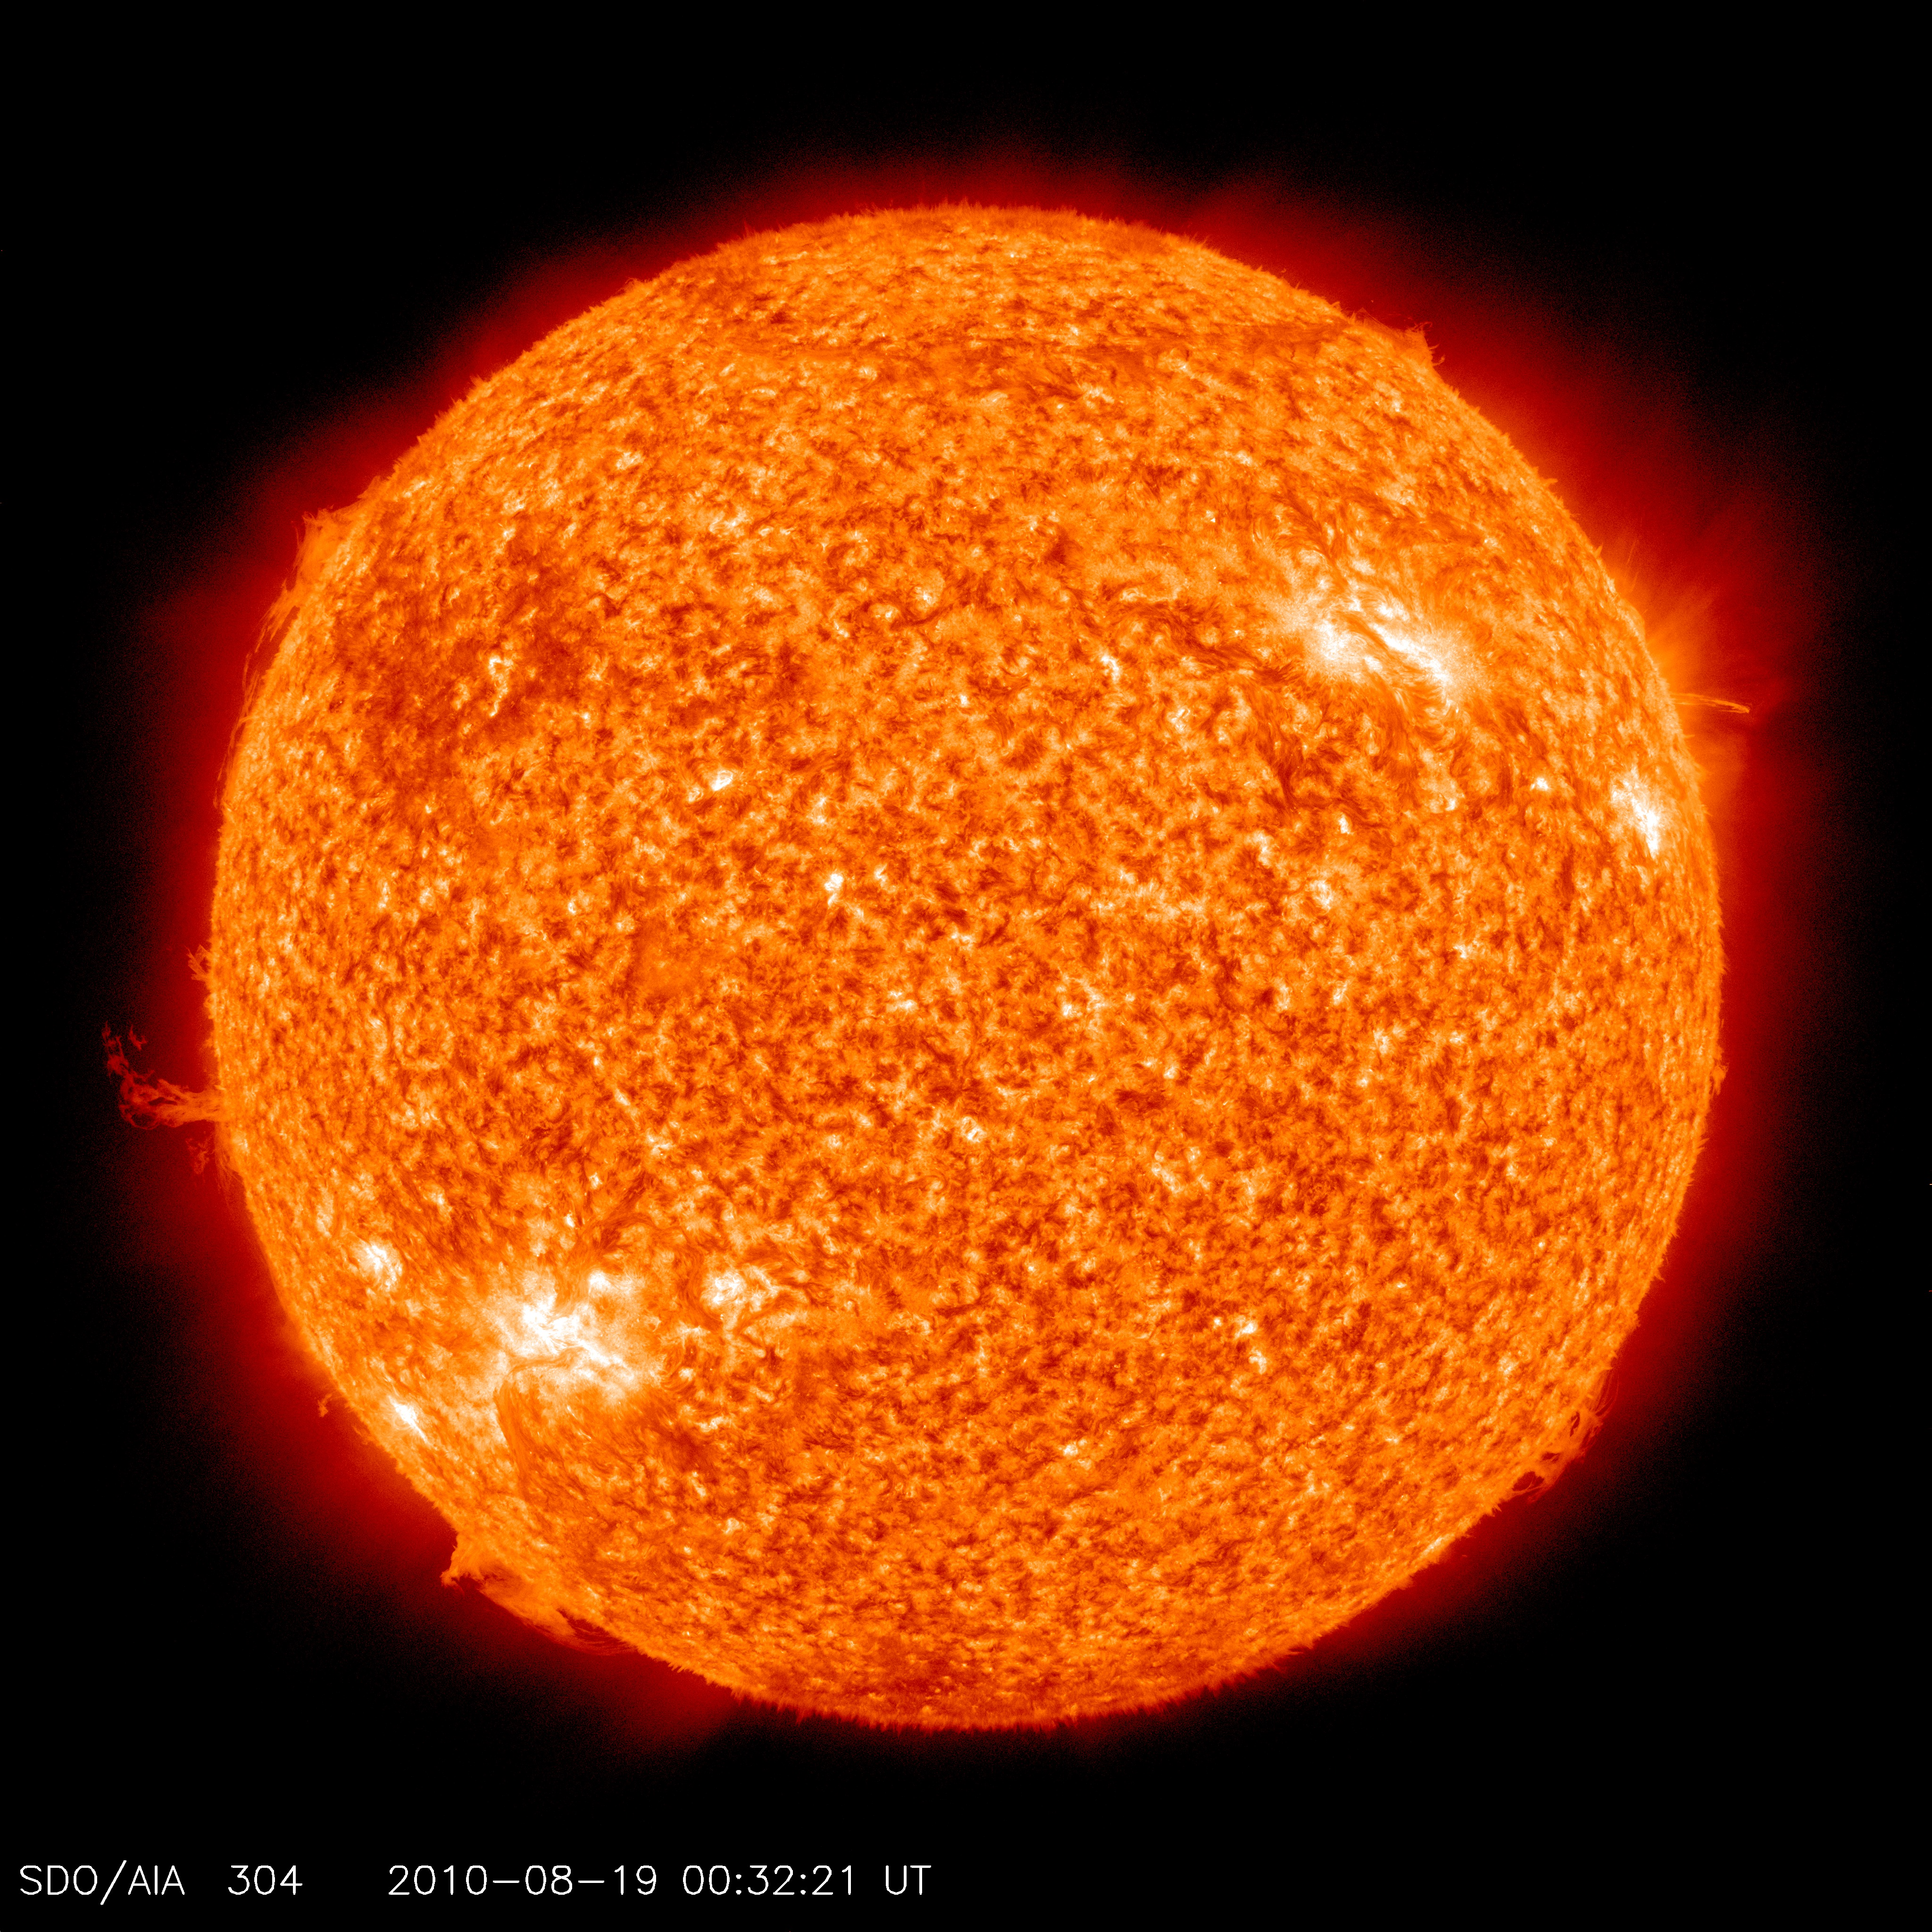
\includegraphics[width=0.5\textwidth]{SunGranulation.jpg}}
    \subfloat[A schematic diagram of convective granulation and how the light from the different parts of the granules are velocity shifted. Source: \citet{2015Haywood}.]{\label{figGranDia}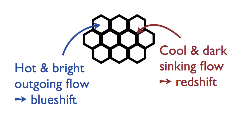
\includegraphics[width=0.5\textwidth]{Granules.png}}
    \caption{}
    \label{figGranSpots}
\end{figure}

Granulation: The convective motion of plasma in the photosphere appears visually as bright and dark cells on the surface of the star (Figure\,\ref{figGranPhot}). This produces blueshifted light in the middle of a granule as the plasma is rising towards the observer, and redshifted light in the intergranular lanes between granules where the plasma is sinking (Figure\,\ref{figGranDia}). In a convective cell there will be the same amount of plasma moving upwards as downwards; however, the rising plasma is hotter and less dense than the sinking plasma. Therefore the granular cells occupy more surface area than the intergranular lanes. The light we see will be the combination of both of these processes and will have a net blueshift. For the Sun this is around 200 ms$^{-1}$ \citep{2010Meunier}. These convective cells of gas range in scale from small (mesogranules) to large (supergranules) with diameters ranging from 150\,km to 2,500\,km and lifetimes from 30 minutes up to a day. \\

Oscillations: Convection is also known to drive acoustic oscillations that move through the star similar to earthquakes in the Earth \citep{1980Cox}. These oscillations were first seen in the Sun \citep{1962Leighton}, and later on observed in other stars. One type, pressure-mode waves\citep{1941Cowling}, travel through the chromosphere, alternating between compressing and expanding the plasma. In the Sun, these oscillations last approximately 5 minutes \citep{1962Leighton}, and are predicted to last from 20-180 minutes in M-dwarfs \citep{2019Rodriguez}.\\

Starspots: Convection will push the magnetic field lines out past the surface of the photosphere into the corona and back down again, producing coronal loops. An illustration of this can be seen in panel \textit{c} of Figure\,\ref{figDynamo}. At the intersection of the coronal loop and the surface of the photosphere we see starspots, which are regions of the surface of a star that are cooler and darker than the surrounding area. Starspots move in position over time as the magnetic field that produced them moves. The concentrated magnetic flux of the loop suppresses convection in the affected area of the photosphere and reduces the surface temperature. The change in temperature can be up to 2000\,K in late F and early G stars and 200\,K for M stars \citep{2009Strassmeier}. Each coronal loop has two points of intersection with the photosphere, and it produces two starspots, one with a north magnetic field and the other with a south magnetic field. As starspots are a byproduct of the magnetic cycle of the star, the number of starspots seen increases as distortion in the magnetic field increases, and will decrease once the polodial magnetic field re-establishes itself. This periodic increase and subsequent decrease in the number of spots is known as the stellar magnetic cycle. One of the earliest investigations of sunspots was by \citealt{1844Schwabe}, while \citealt{1904Maunder} observed that the number of sunspots were at a maximum at mid-latitudes, and decreased as the spots moved towards the equator. For the Sun this cycle has a period of around 11 years, however for M-dwarfs, the magnetic cycle is not only shorter, but also depends on how fast the star is rotating. For fast rotating M-dwarfs (periods of less than a day), the magnetic cycle can last roughly a year, while the slower rotating M-dwarfs have cycles of approximately four years\citep{2019Kuker}. At the maximum of the stellar magnetic cycle, there can be significant numbers of starspots that cover a significant fraction of the visible surface of the star. Early estimates of starspot coverage in cool stars such as M-dwarfs predicted coverage rates of up to 64\%\citep{1995Neff}, however further work has this estimate closer to 40\%\citep{2004Oneal}. Sufficient numbers of starspots will decrease the amount of light coming from the star by a noticeable amount. At the maximum of the solar magnetic cycle, sunspots reduce the light from the Sun by 0.1\% \citep{2006Carroll}.\\

Faculae: Accompanying starspots are regions of the photosphere that appear slightly brighter and hotter (up to 100\,K) than the regular (non-active) regions of the atmosphere. They are most visible at the limbs of the star. Faculae occur in the photosphere as bright points and are often found near starspots, indicating some connection between them, but can also be seen in extended groups independent of a starspot. \citet{1976Spruit} proposed the ``bright wall'' model to explain faculae. Essentially magnetic flux will make the plasma in a convection cell less opaque, allowing a view deeper into the photosphere. Observations of faculae on the Sun by \citet{1978Hiryama} found that faculae can last up to a few hours. One interesting feature of note is that at the time of sunspot maximum, faculae emit enough light to overcome the deficit from the starspots and actually increase the total amount of light seen \citep{2004Keller}.\\

Plages: The chromospheric counterpart to faculae are plages. Plages are larger in scale than faculae and often herald the formation of starspots in a region. They are produced by the interaction of magnetic fields with pockets of plasma that are higher in density than the rest of the chromosphere. Plages can be detected in a spectrum as an emission component, primarily in Ca H \& K and H$\alpha$, and they are the source of H$\alpha$ emission near starspots \citep{2006Carroll}.\\

\begin{figure}
    \captionsetup{width=.45\textwidth}
    \subfloat[A zoomed in photo of the Sun showing starspots (dark regions) with faculae (light regions) surrounding them. Source: https://solarscience.msfc.nasa.gov/feature1.shtml.]{\label{figSunspot}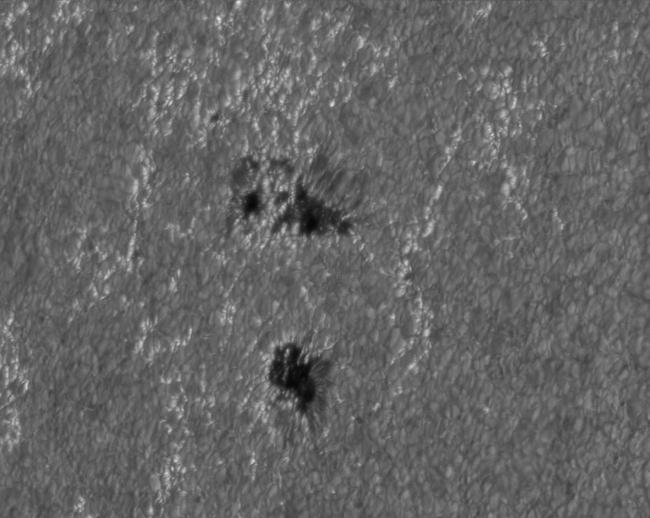
\includegraphics[width=0.555\textwidth]{faculae.jpg}}
    \subfloat[An X-ray image of flares on the surface of the 
    Sun in 2005 from the TRACE satellite. Source: https://www.nasa.gov/mission\_pages/swift/bursts\newline/monster\_flare.html.]{\label{figFlare}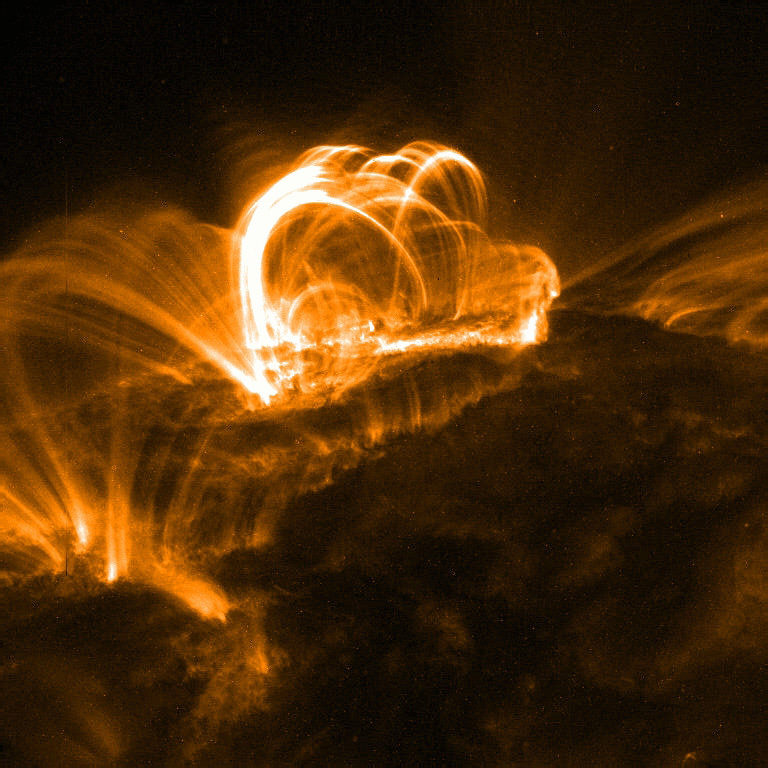
\includegraphics[width=0.445\textwidth]{162169main_Trace_solar_flare_lg.jpg}}
    \caption{}
    \label{figStellActiv}
\end{figure}

Flares: Flares are the result of magnetic reconnection, where the interaction of magnetic field lines converts heat into kinetic energy, producing highly accelerated electrons that will interact with the plasma of a star, resulting in a sudden, but short-lived, release of energy, increasing the brightness of the star by several magnitudes across a wide range of wavelengths \citep{2012Schmidt} and a significant increase in emission line strength. A typical example of the effect of flares on a spectrum is seen in Figure \ref{figFlareDia}. Specific lines in the spectra of EV Lac are significantly stronger while the star is flaring. The black line represents the flux when the star is not flaring and the red line is the while the star is flaring. In M-dwarfs the increase in emission can last for a few minutes to hours \citep{2011Hilton}. Afterwards, the flux returns to normal. While the duration of a flare is relatively short, they have been shown to be quite frequent in some active stars. \citet{2014Hawley} analysed M-dwarf Kepler data and found that the number of flares per day was inversely proportional to the strength of the flares.\\

\begin{figure}
    \centering
    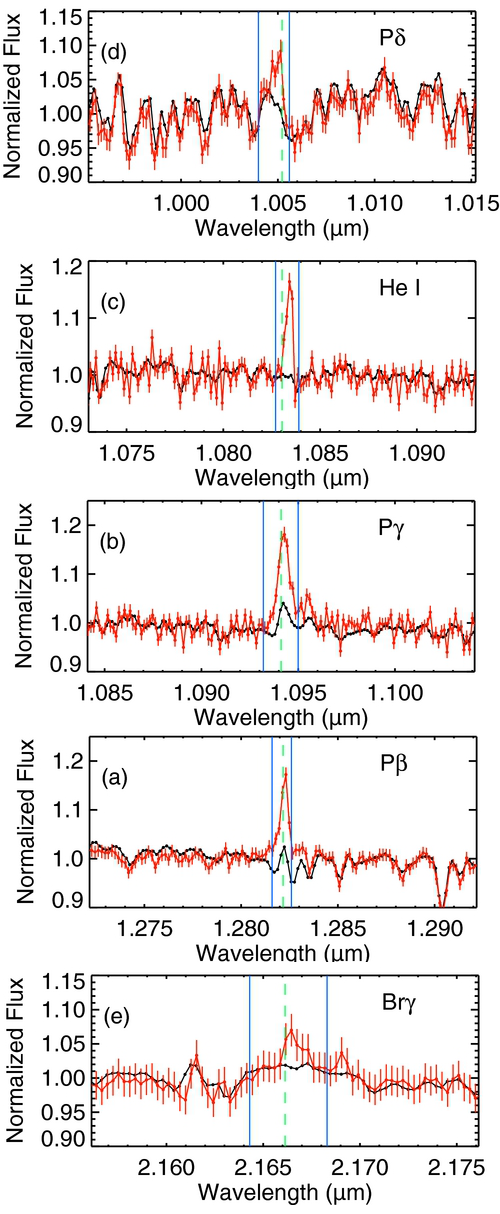
\includegraphics[width=\textwidth,height=0.95\textheight,keepaspectratio]{Flare2.png}
    \caption{Regions of the spectrum of EV Lac in and out of flare. A quiescent (non flaring) spectrum is shown in black and a spectrum taken while the star was flaring is in red. Source: \citet{2012Schmidt}.}
    \label{figFlareDia}
\end{figure}

\subsubsection{Influence of variability on exoplanet detection methods}
\label{secVarInfluence}
The timescale of these changes to the stellar surface will vary from minutes to days, depending on the mechanism producing them. Short duration variation will produce the low level, short period, signals seen in a periodogram like Figure\,\ref{figHD85512Power}. Longer duration variation may correspond to periodicities that can be falsely attributed to a potential exoplanet. For example, Kapetyn's star (GJ191) was observed by the HARPS team in 2014 and they reported two planets with periods of 48.6 and 121.5 days \citep{2014Anglada-Escude}. Further analysis by \citet{2015Robertson} found that the 48.6 day planet was most likely periodic magnetic activity causing a false radial velocity signal.\\

An individual convective granule is expected to add 1-2~kms$^{-1}$ of jitter; however, the fluctuations from the granules obey Poisson statistics and so the total radial velocity contribution by granules is dependent on the square root of the number of granules. The Sun has roughly 1 million granules visible at any one time, so the radial velocity noise from convective granulation scales down to 1-2~ms$^{-1}$ \citep{2003Lindegren}. Convective granules can last from minutes up to an hour, depending on size. Therefore \citet{2008Otoole} proposed that the simplest way to mitigate convective granulation jitter was to take several observations over the same night and take a mean spectrum, which would average out the fluctuations.\\

Pressure mode stellar oscillations will stretch and compress the plasma they travel through on timescales of 5 to 15 minutes \citep{2000Schrijver}. This will introduce a jitter of 0.01-0.4 ms$^{-1}$ into any radial velocity measurements, depending on the class of star. The amplitude of the jitter was found to be related to the luminosity/mass ratio \citep{2004Christensen-Dalsgaard}, so for cool stars like M-dwarfs, the jitter will be at the lower end of this range. By setting a minimum exposure time of 15 minutes, \citet{2011Dumusque} proposed that the radial velocity influence of the oscillations would be avoided.\\ 

M-dwarfs are known to be quite active, with starspots as a significant source of jitter. The light we observe comes from the whole visible face of the star. As the star is rotating, the light from the side rotating towards us will be blueshifted, and the light from the side rotating away will be redshifted. However, when a starspot rotates into view, the light from the blueshifted side will be reduced due to the spot-affected area being cooler than its surroundings. This imbalance in the amount of light coming from each side will also break the symmetry of a line profile. This effect is illustrated in Figure\,\ref{figSpotRotation}. Initially the starspot is not visible and the profile of the spectral line is symmetrical. As the starspot rotates into view, it suppresses some of the blueshifted flux, changing the profile of the blue side of the line and producing an asymmetry. Once it is directly in our field of view the symmetry is restored, but only because the flux is suppressed evenly across both sides of the line, producing a weaker, but symmetrical line. Once the spot begins to rotate away from view, the redshifted light is suppressed. Starspots on the Sun, which is considered to be somewhat quiescent compared to other main-sequence dwarfs, have been found to add around 0.65 ms$^{-1}$ of jitter \citep{2009Makarov}. The magnitude of this jitter is expected to be greater for more active stars such as M-dwarfs, and for faster rotating stars.\\

\begin{figure}
    \centering
    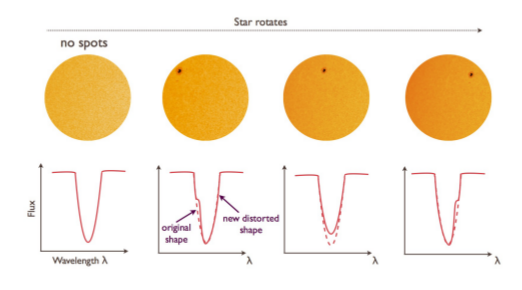
\includegraphics[width=0.8\textwidth]{SpotRotation.png}
    \caption{As a starspot rotates into view, it will first block the blueshifted side of the star, then cross the face to the redshifted side before moving out of view. Source: \citet{2015Haywood}.}
    \label{figSpotRotation}
\end{figure}

Faculae and plages affect the plasma of the star in a similar manner to starspots. While their influence on the temperature of the plasma is not as strong, they are spread out over a much larger area. Models of the Sun by \citet{2010Meunier} indicate that plages will add 8-10~ms$^{-1}$ of jitter, and a study of 171 G, K, and M stars by \citet{2020Hojjatpanah} found jitter on similar scales for faculae.\\

As the CCF is based of the profile of lines in a spectrum, the sudden increase in strength of select emission lines from flares will impact the CCF and therefore the radial velocity. The jitter produced will on the order of tens of ms$^{-1}$ \citep{2009Reiners}. However, flares occur sporadically and have timescales of minutes, so a it is unlikely for more than a single observation to capture flaring activity. Emission in the core of the H$\alpha$ line is particularly sensitive to flares, making it a useful tool to identify and removed affected observations.\\

While strong chromospheric and photometric activity in stars are known to produce detectable radial velocity variations, work by \citealt{2014Bastien} found measurable radial velocity variations in chromospherically and photometrically quiescent stars. They combined transit photometry from the Kepler survey, and spectra from the California Planet Search\footnote{$http://exoplanets.org/exoplanets_pub.html$} for 12 stars with low S-index measurements (see Section\ref{secVarQuant} for details on S-indices). For each star, radial velocities were measured for all spectra and the standard deviation across 2-hour bins was determined. They found radial velocity variations of several ms$^{-1}$, with one star varying by almost 136\,ms$^{-1}$! Further analysis found that the radial velocity variations strongly correlated with the number of significant peaks in the Fourier power spectrum of the photometric variability (where `significant' means the strongest peak and all peaks with a power \textgreater10\% of the strongest peak). They suggested that faculae might dominate in slowly rotating stars, producing low photometric activity, but more significant radial velocity variations.
\subsubsection{Quantifying the impact of variability}
\label{secVarQuant}
Any radial velocity measurement taken from a spectrum will include contributions from jitter. The greater the amount of jitter, the further away any single measurement of the RV can be from the ``true'' velocity, and the harder it will be to determine small amplitude periodic variations in radial velocity. While some jitter can be mitigated by the choice of suitably long exposure times and other observing strategy choices, other jitter mechanisms are unavoidable. Some stars will have moderate to low levels of activity that have little influence on the quantities we are trying to measure, while other stars will be so strongly affected by variability that the precision of radial velocity measurements required to detect an exoplanet above the noise will be impossible. Identifying these stars is important so that optimal observing targets can be prioritised. Metrics that can predict the variability of a star are valuable tools. \\

\begin{figure}
    \centering
    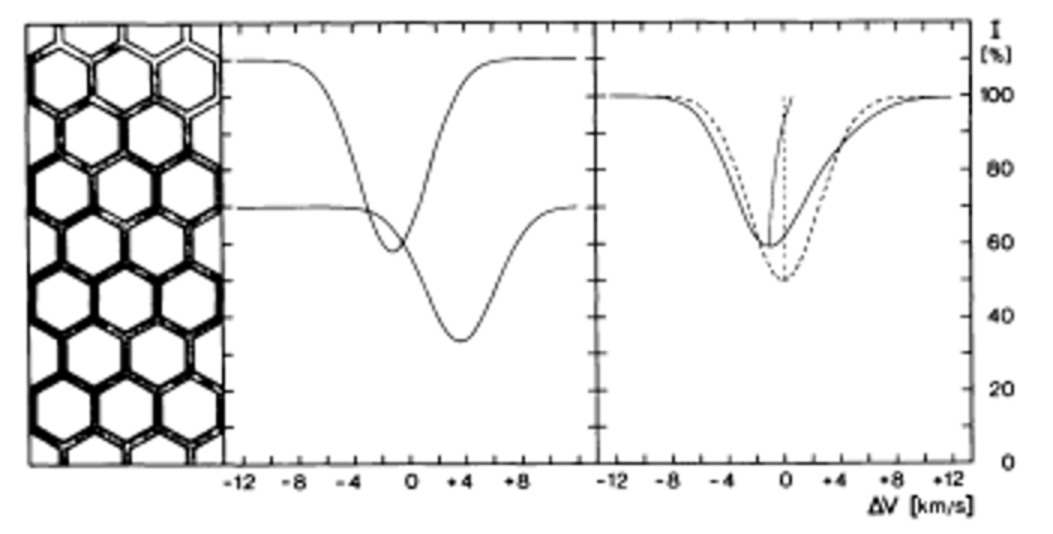
\includegraphics[width=0.8\textwidth]{LPV_convection.pdf}
    \caption{Schematic illustration of how convective granules affect the profile of spectral lines. Source: \citet{1981Dravins}.}
    \label{figLineProfile}
\end{figure}

An idealistic view of a stellar spectral line could be thought of as Lorentzian and symmetric. However, processes like convection will break that symmetry. \citet{1981Dravins} modelled the effect of granulation on the profile of a spectral line and Figure\,\ref{figLineProfile} is an example. The left panel is a diagram of the convective granules and the intergranular lanes. Their model assumed that 75\% of the visible face of the star was covered with granules, with an upward flow in the granules moving at 1.2 kms$^{-1}$ and the downward flow in the intergranular lanes moving at 3.6 kms$^{-1}$. Each of these flows produces a different line profile in the centre panel, with the stronger and bluer profile produced by the granules, and the weaker and redder profile coming from the intergranular lanes. The solid line in the right panel is the sum of both of these profiles, while the dashed line is the profile if there were no interference from granulation. Comparing the two profiles, it is obvious that the profile affected by convection is asymmetrical and bluer when compared to the unaffected profile. Changes to the line asymmetry over time will produce changes in the radial velocity over the same timescale. As the CCF represents the average line shape in the spectrum, measuring the change in the shape of the CCF over time is a useful metric of stellar activity.\\

\begin{figure}
    \centering
    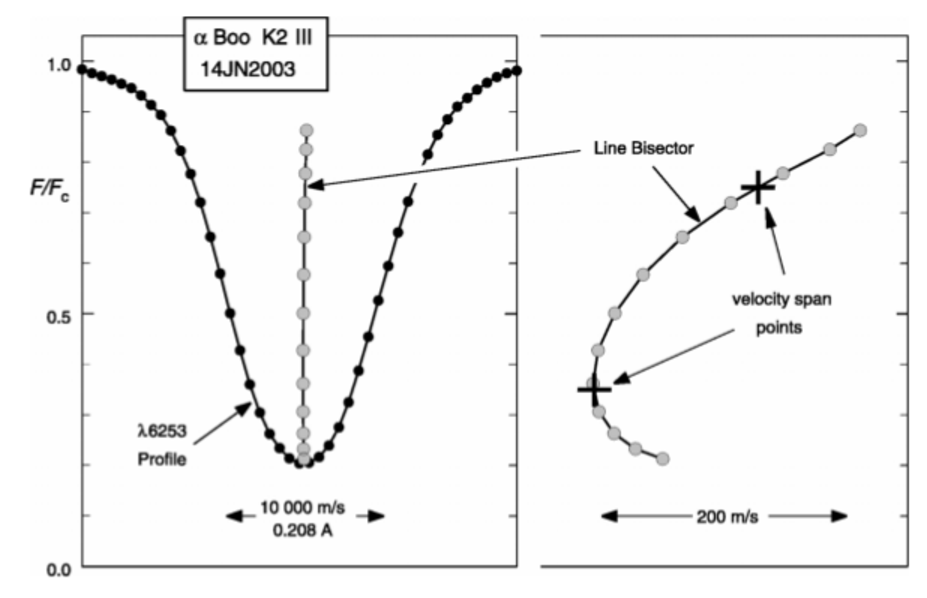
\includegraphics[width=0.8\textwidth]{Bisector.pdf}
    \caption{Line profile and bisector of the Fe line at 6253\,\AA\: in the spectrum of Arcturus. The right panel is zoomed in on the line bisector. Source: \citet{2006Gray}.}
    \label{figBis}
\end{figure}

Another tool for quantifying variability is the line bisector. If we were to sample a line in wavelength space, or a CCF in velocity space, at multiple points along the y-axis (the points in Figure\,\ref{figBis}) and obtain the the horizontal mid-point at each point (the grey points in the figure), then the trend of these mid-points would carry information about the shape of the line, and therefore about the levels of activity present. For a perfectly quiet star, we could assume that the bisector would be vertical; however, the convective granulation that produced the asymmetrical line profile will result in a curved bisector, seen in the right panel of Figure\,\ref{figBis}. There are multiple ways of using the bisector, including the bisector velocity span \citep{1988Toner} and the Bisector Inverse Slope (BIS) of the CCF \citep{2001Queloz}. If the bisector is determined across multiple observations, these methods can provide a measure of how the surface of the star is changing over time that can be correlated with radial velocity to determine whether the periodic changes of a specific period are due to stellar activity.\\

\begin{figure}
    \captionsetup{width=.8\textwidth}
    \subfloat[]{\label{figNaDfull}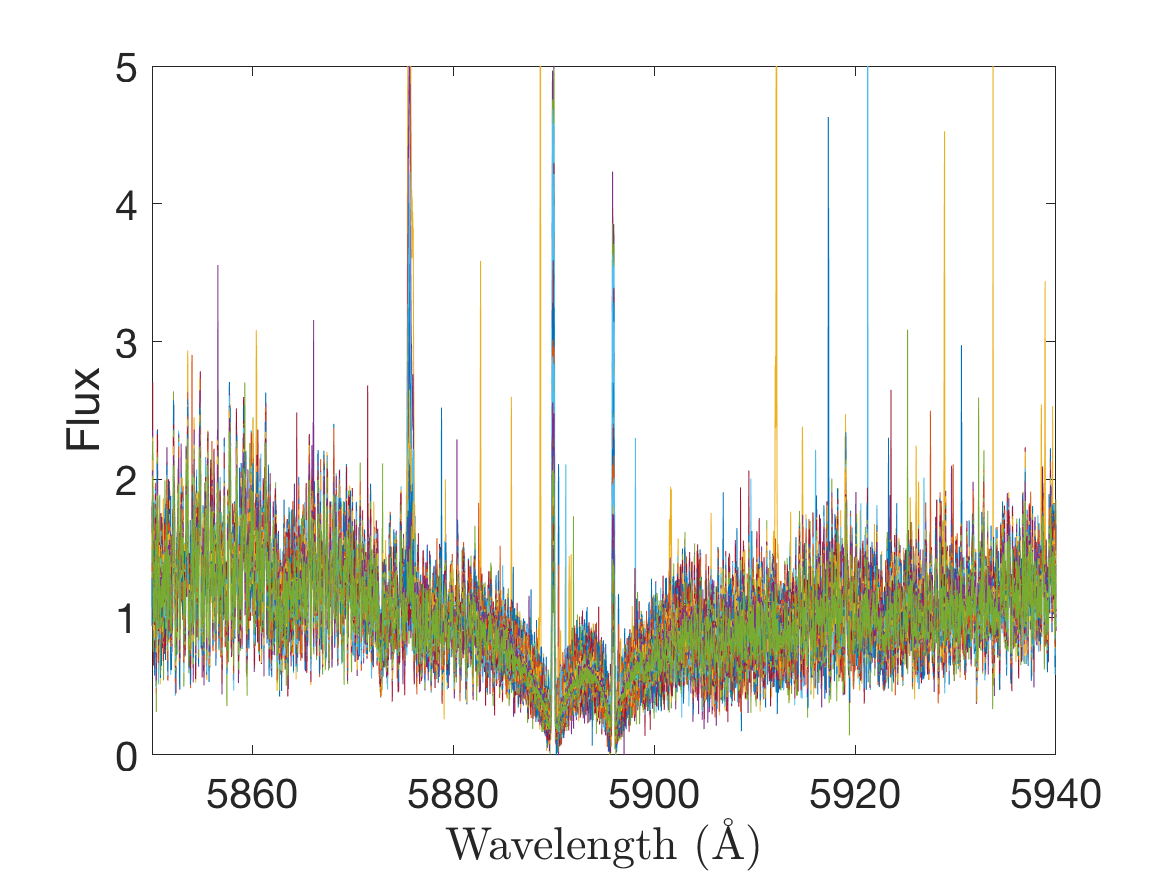
\includegraphics[width=0.5\textwidth]{NaDfull.png}}
    \subfloat[]{\label{figNaDzoom}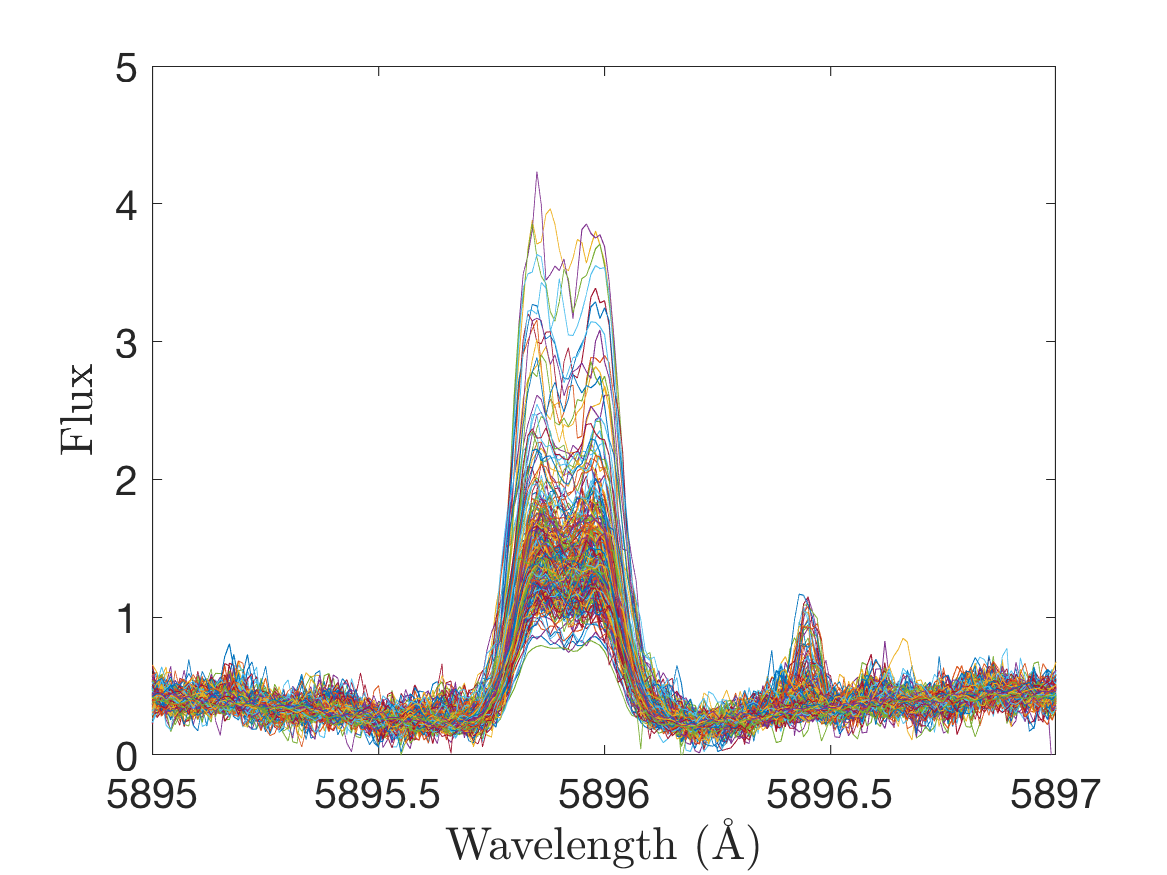
\includegraphics[width=0.5\textwidth]{Gl551_NaD_example.png}}
    \caption{Continuum normalised HARPS Spectra of GL551, focusing on one of the Na\,\textsc{i} D lines. In the core of the absorption line are two emission features that vary from observation to observation.}
    \label{figNaD_line}
\end{figure}

A stellar atmosphere will produce absorption and emission features in the spectrum of the star. Changes to the structure of the atmosphere will result in a change to the features in the spectrum, and therefore a change to any radial velocity measurement that uses those features. Several strong absorption lines have emission features at their cores that vary in strength over time, and the magnitude of this change correlates with changes in the radial velocity of the star. The most commonly used lines are Ca\,\textsc{ii} H (3968.47\,\AA) \& K (3933.66\,\AA), H\,\textsc{$\alpha$} (6562.808\,\AA), and Na\,\textsc{i} D doublet (5889.95\,\AA \& 5895.92\,\AA). An example of this is Figure\,\ref{figNaD_line} in which a Na\,\textsc{i} D emission feature can be clearly seen to vary in strength over a number of observations.\\

\begin{figure}
    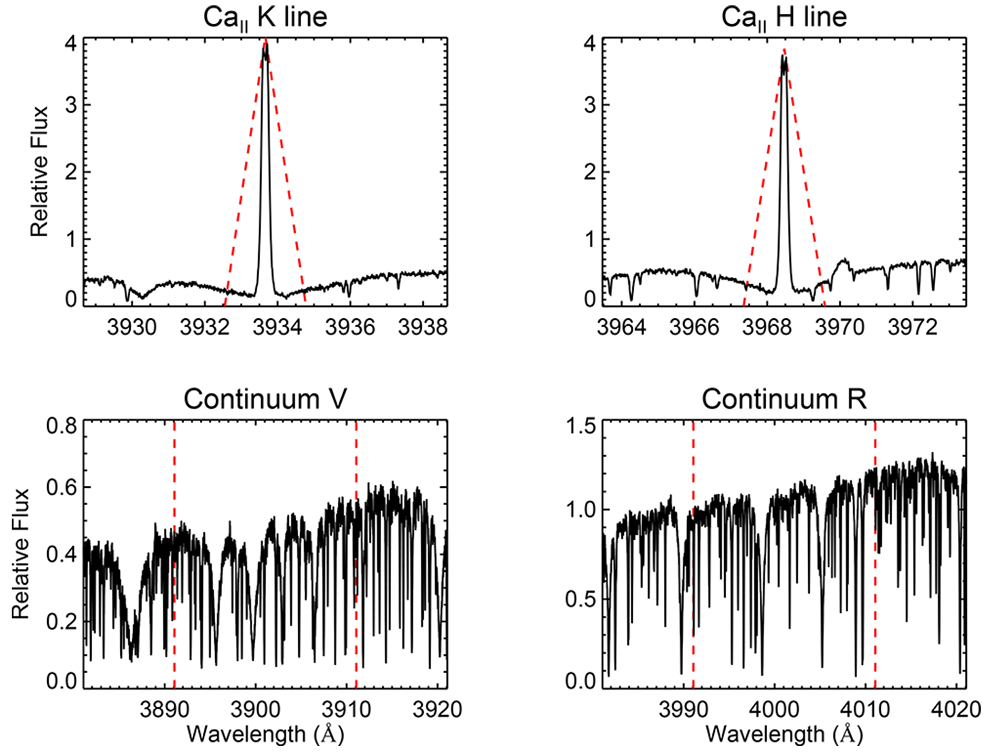
\includegraphics[scale=0.5]{MtWilson.png}
    \caption{Small regions of the spectrum of GJ176, with red dashed lines indicating the bandpasses for the Mount Wilson S-index (Equation\,\ref{eqSind}). The upper panels show the K and H feature bands, and the lower panels show the violet and red sidebands. Source: \citet{2015Suarez}.}
    \label{figLPVexample}
\end{figure}

The Ca\,\textsc{ii} H \& K lines are useful as they are strong and are in the visible wavelength range. The absorption comes from the photosphere, while the emission at the core of the line is produced in the upper photosphere and lower chromosphere, making it an excellent probe of those regions. \citet{1968Wilson} first correlated flux across the Ca\,\textsc{ii} H \& K lines to chromospheric activity by looking at the spectra of 91 main sequence stars over a roughly 10 year period. The product of this work was the Mount Wilson S-index (Equation \ref{eqSind}; \citealt{1978Vaughan}) which uses the flux in 1\,\hbox{\AA} passbands across each of the Ca\,\textsc{ii} H \& K lines. To normalise the measurement, they took the flux, $f(\lambda)d\lambda$, from 25\,\hbox{\AA} sidebands on the violet and red sides of the two calcium lines. Figure\,\ref{figLPVexample} displays the regions containing the passbands and sidebands used in the S-index. Since that time different groups have adapted the wavelength regions to better suit the type of star they are looking at or to refine the selection of the emission feature. For example, \citet{2011Gomes} decreased the line bandpass from 1\,\AA\:to 0.6\,\hbox{\AA} to exclude the line wings, which contain flux from the photosphere, and shifted to 20\,\hbox{\AA} sidebands centred around 3900\,\hbox{\AA} and 4000\,\hbox{\AA}.\\

\begin{equation}
	S_{HK} = \alpha\frac{\int_{3933.36}^{3933.96}f(\lambda)d\lambda+\int_{3968.17}^{3968.77}f(\lambda)d\lambda}{\int_{3890}^{3910}f(\lambda)d\lambda+\int_{3990}^{4010}f(\lambda)d\lambda}
	\label{eqSind}
\end{equation}

One issue with the S-index is that the values obtained are specific to the instrument and spectral type of the star. As such, a normalisation factor $\alpha$, based on observations of standard stars taken on the same night as the observation, is used to remove this dependence. See \citet{1982Middelkoop} for details of the normalisation factor. An alternative index that is independent of instrument and spectral class, $R^{\prime}_{HK}$, was developed by \citet{1984Noyes}. The main advantage of the $R^{\prime}_{HK}$ index (Equation\,\ref{eqRind}) over the S-index is that it measures activity in the lower chromosphere only, unlike the S-index which measures activity in both the upper photosphere and lower chromosphere. This is achieved by measuring the flux across the H and K lines as per the S-index, subtracting the photospheric flux from a quiescent reference star, leaving only the chromospheric flux $f^{\prime}(\lambda)d\lambda$, and replacing the denominator with $\sigma T^{4}$. The logarithm of this index is often reported as log($R^{\prime}_{HK}$).\\

\begin{equation}
	R^{\prime}_{HK} = \frac{\int_{3933.36}^{3933.96}f^{\prime}(\lambda)d\lambda+\int_{3968.07}^{3968.77}f^{\prime}(\lambda)d\lambda}{\sigma T^4_{eff}}
	\label{eqRind}
\end{equation}

These indices are commonly used to quantify chromospheric activity across most stars, however cool stars have insufficient flux in the Ca\,\textsc{ii} H \& K lines for $S_{HK}$ or log($R^{\prime}_{HK}$) to be a reliable proxy of stellar activity. Other chromospheric emission lines provide suitable replacement proxies of variability, such as H\,\textsc{$\alpha$} and the Na\,\textsc{i} D lines. H\,\textsc{$\alpha$} is located at the red end of the visible range and is sensitive to activity in the upper chromosphere. \citet{2014Gomes} investigated how useful S$_{H\alpha}$ was as an indicator of long period activity and found that S$_{H\alpha}$ correlated poorly with log($R^{\prime}_{HK}$) for stars with long period activity seen in log($R^{\prime}_{HK}$). The Na\,\textsc{i} D lines pair well with H\,\textsc{$\alpha$} because they all probe the lower to middle chromosphere \citep{2000Mauas}, allowing for full coverage of the chromosphere when both S$_{CaHK}$ and S$_{NaD}$ are determined.\\

\subsubsection{Application of variability indicators to spectroscopic data}
\label{secVarApp}
Once a periodic variation in the radial velocity is detected, the next step is to check that it is not the result of stellar activity. If changes in the radial velocity over time correlate with any of the variability measurements discussed in Section\,\ref{secVarQuant}, then it is highly likely that the periodic radial velocity signal comes from activity and not an exoplanet. For example, Figure\,\ref{figGL433_activity} shows that the radial velocity variations of GL433 (bottom panel) follow a similar pattern over time to an index measuring Na\,\textsc{i} D emission (middle panel). The two quantities have a Pearson coefficient of 0.91, indicating that they are highly correlated and the 1758.09 day period is most likely to be the result of long-term activity.\\

\begin{figure}
    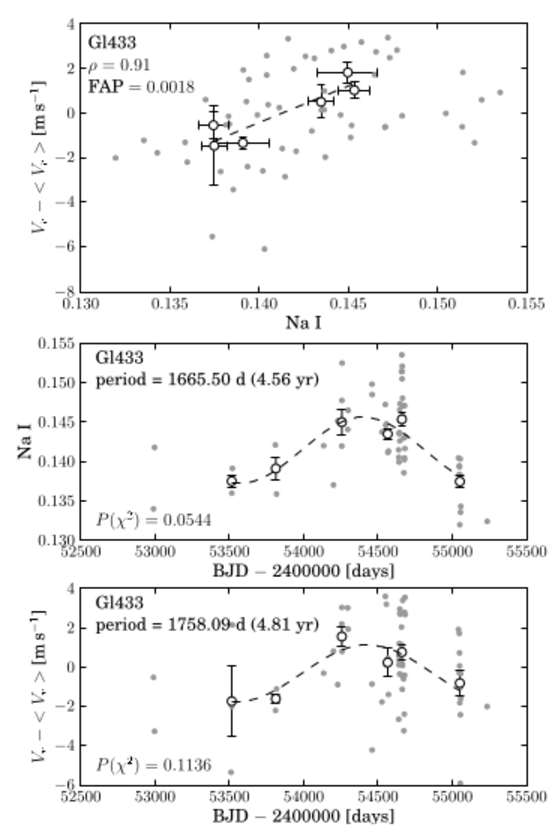
\includegraphics[width=0.8\textwidth]{Gl433_activity.pdf}
    \caption{Radial velocity and Na\,\textsc{i} D index measurements for GL433 (lower panels) and the correlation between the two (top panel). Source: \citet{2012Gomes}.}
    \label{figGL433_activity}
\end{figure}

Additionally, variability measurements can be analysed in parallel with the radial velocities. Taking the example of HD85512 from Section\,\ref{secRVanalysis}, the log($R^{\prime}_{HK}$) and BIS were measured for each observation and the periodograms for those quantities are shown in the middle and bottom panels of Figure\,\ref{figHD85512Periodogram}. There are peaks of significance at 58, 69, 85, and 300 days in the radial velocity panel, but the strengths of these peaks changes in the other two panels. The 300 day peak is the only one to have significant strength in all three measurements. Since the log($R^{\prime}_{HK}$) and BIS measurements are proxies for variability, the 300 day radial velocity peak is more likely to be the product of variability than a planet.\\

\begin{figure}
    \centering
    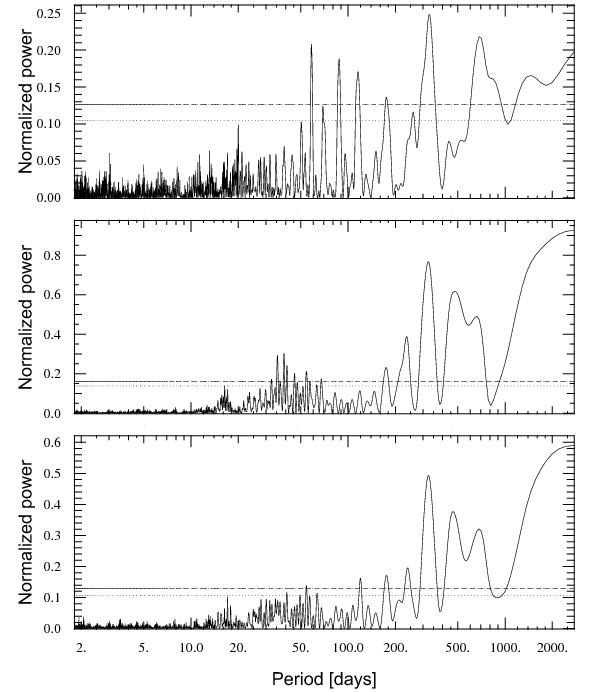
\includegraphics[width=0.8\textwidth]{HD85512_Periodogram.jpg}
    \caption{Periodograms of HD85512 produced from the (top) radial velocity, (middle) log($R^{\prime}_{HK}$), (bottom) line bisector BIS. Peaks at 58, 69, 85, and 300 days are found to be significant in the radial velocity measurements, and the 300 day period is also strong in the log($R^{\prime}_{HK}$) and BIS measurements. Dotted and dashed horizontal lines indicate FAP of 1\% and 10\% respectively. Source: \citet{2011Pepe}}
    \label{figHD85512Periodogram}
\end{figure}

\subsubsection{Radial velocity spectrographs}
\label{secSpecSurveys}
Exoplanet-focused spectroscopic surveys obtain multiple spectra of a sample of stars over a long enough time period to measure velocities over an orbit, although multiple orbits are preferable. These velocities are then analysed to look for periodic signals indicating the potential presence of exoplanets around the star. Detecting \textless1 ms$^{-1}$ radial velocities requires spectrographs built with high resolution (\textgreater 80,000) and intrinsic stability in mind. Two recent examples of exoplanet-focused spectrographs are HARPS and ESPRESSO.\\

Some of the most accurate radial velocities in recent time have come from the European Southern Observatory (ESO) High Accuracy Radial velocity Planet Searcher (HARPS; \citealt{2003Mayor}) spectrograph using the 3.6m telescope at La Silla, Chile. HARPS is a fibre-fed, cross-dispersed echelle spectrograph that was designed to be highly stable, allowing for radial velocities with precision of down to 1ms$^{-1}$. The spectrograph is placed inside a vacuum chamber which reduces the amount of spectroscopic line drift from atmospheric pressure changes to less than 0.1 ms$^{-1}$ \citep{2004Rupprecht}. Additionally, the temperature of the chamber is kept stable to 0.01\,K, and simultaneous Thorium-Argon wavelength calibration is used. The HARPS spectrograph has been used for multiple observing campaigns and has resulted in the detection of many exoplanets. Some highlights include the detection of a 1.7\,M$_\oplus$ exoplanet around GL581 \citep{2009Mayor}, one of the smallest detected exoplanets at the time, and a \textgreater1.2\,M$_\oplus$ exoplanet around Proxima Centauri \citep{2016AngladaEscude}, a star which is known to be active, making a confident detection of a planet difficult.\\

The Echelle Spectrograph for Rocky Exoplanet - and Stable Spectroscopic Observations (ESPRESSO; \citealt{2013Pepe}) is the successor to HARPS and saw first light in September 2016. It is a high-resolution (R $\sim$200,000), ultra-stable spectrograph with a wavelength coverage of 380\,-\,686 nm, and is installed on the Very Large Telescope (VLT). Due to the four 8.2 m telescopes comprising the VLT array, and improvements in laser-comb technology, ESPRESSO targets a precision of 30 cms$^{-1}$, a substantial improvement on HARPS. One of the significant results from ESPRESSO so far is the confirmation of a exoplanet around Proxima Centauri. \citet{2016AngladaEscude} found a 1.3 M$_\oplus$ exoplanet orbiting Proxima Centauri using radial velocities from HARPS and UVES\,\citep{2000Dekker} spectra. As Proxima Centauri is known to be very active, follow-up observations were required to confirm this detection as more data points allow for a better sampling of the orbit. The ESPRESSO data found the mass to be 1.29\,$\pm$\,0.13 M$_\oplus$ and the orbital period to be 11.218\,$\pm$\,0.029 days.

\section{Surveys relevant to this work}
\label{secSurvey}
There are multiple large-scale spectroscopic and photometric surveys that, while not specifically focused on exoplanets, have been used in the research presented in this thesis. Their key parameters are summarised here.\\

The Two Micron All Sky Survey (2MASS; \citealt{2006Skrutskie}) was a ground-based, full-sky photometric survey that used two 1.3 m telescopes, one in Chile and the other in Arizona, USA to obtain photometry of 470 million objects from 1997 to 2001. One of the major 2MASS data products was a point source catalogue that gives a comprehensive photometric view of stars in the Milky Way. 2MASS obtained photometry in the infrared J, H and K$_s$ passbands (1.2, 1.7 and 2.2\,$\mu$m).\\

The Wide-field Infrared Survey Explorer \citep[WISE;][]{2010Wright} is a satellite that was built by NASA to survey the whole sky at $3.4, 4.6, 12$ and $22 \mu m$ (W1, W2, W3, W4). The four WISE passbands are designed to be sensitive to emissions from different types of objects in the sky. M-dwarfs radiate sufficient flux across the wavelengths covered by W1 and W2 for these passbands to provide useful information. However, W3 and W4 occur at very red wavelengths, with insufficient flux to provide information about M-dwarf characteristics. Over 7 months in 2010, the WISE satellite obtained photometry of over 563 million objects. The full data set includes basic position information, photometric magnitudes for W1, W2, W3 and W4, and where possible, cross-matched J, H, and K$_s$ magnitudes from 2MASS.\\

\textit{Gaia} \citep{2016Gaia} is a space telescope and the successor to the HIgh Precision PARallax COllecting Satellite \citep[HIPPARCOS;][]{1981Kovalevsky} satellite. Its primary mission is to obtain photometry and a 5-component astrometric solution (right ascension, declination, proper motions, and parallax) for approximately 1 billion objects over a 5 year mission (2014-2019). In 2018 the \textit{Gaia} mission was assessed and was approved for an extension for as long as its on-board fuel lasts, which is predicted to be into 2024 \citep{2019Brown}. \textit{Gaia} will typically acquire 70 observations of each star during its operational phase, with the precision in the derived quantities increasing along with the volume of data. \textit{Gaia} collects photometry in a broad optical G passband and in narrower Bp and Rp filters. The precise and frequent astrometric measurements mean that highly accurate parallaxes and proper motions can be measured for most, if not all, of the stars it observes. Parallaxes are expected to be obtained with a precision of 9-11\,$\mu$as for stars brighter than V = 10, 10-27\,$\mu$as at V = 15, and 100-350\,$\mu$as at V = 20. \textit{Gaia} also collects objective prism spectra and determines radial velocities for stars brighter than V = 15 with an accuracy of between 1\,-\,15\,kms$^{-1}$.\\

The GALactic Archaeology with HERMES (GALAH) survey \citep{2021Buder} is a high-resolution (R\,=\,28,000), multi-object spectroscopic survey that is observing 1 million Milky Way stars using the High Efficiency and Resolution Multi Element Spectrograph (HERMES) spectrograph \citep{2015Sheinis}. The aim of the survey is to study the history of star formation, chemical enrichment, and minor mergers in the Milky Way. Because this requires detailed chemical abundance measurements, the HERMES cameras cover four wavelength regions that deliver information on stellar parameters and 30 different elements from all major nucleosynthetic channels. The bandpasses are blue (4718-4903$\hbox{\AA}$); green (5649-5873$\hbox{\AA}$); red (6481-6739$\hbox{\AA}$) and infrared (7590-7890$\hbox{\AA}$). The spectra are reduced in a pipeline described by \citet{2017Kos} and analysed using Spectroscopy Made Easy \citep[SME;][]{1996Valenti}. Chapter\,\ref{chapGALAH} details the use of M and K dwarf spectra from this survey to identify active spectral lines across the GALAH bandpasses and investigate the effect of that activity on abundance determination.

\section{Research motivation}
M-dwarfs are excellent candidates as hosts of small rocky planets orbiting in the habitable zone. There are a large number of absorption lines in their spectra, and they tend to rotate slowly, facilitating precise measurements of their radial velocities. Their habitable zones are located relatively close to the star, increasing the detectability of planets orbiting at those distances. But as mentioned previously, there are several obstacles to overcome:\\

Identifying an M-dwarf typically requires a spectrum. For a small sample of stars, obtaining this information is not a difficult task. However, for larger samples, especially for large surveys, this would require significant telescope time. A method by which we could identify M-dwarfs with minimal additional observations would be beneficial. This work, originally published in the Monthly Notices of the Royal Astronomical Society \citep{2019Bentley}, is explored in Chapter\,\ref{ChapPhot}.\\

Additionally, M-dwarfs are known to be very active early in their lifetimes. While active stars can provide useful information about how planets develop in extreme environments, high levels of stellar activity disrupt our ability to detect exoplanets through radial velocity, making them less useful for planet searches. So for efficiency, active stars will need to be identified and not observed further. Existing indices for the Ca\,\textsc{ii} H \& K, H\,\textsc{$\alpha$}, and Na\,\textsc{i} D features are known to correlate with stellar activity, but they are only useful if there is sufficient flux in the spectrum for at least one of these lines. An index that works across a broader range of wavelength would be more useful, especially if it used the same wavelength range we use to measure the radial velocity. Chapter\,\ref{chapISV} develops such a method.\\

Once these selection methods have been developed, they need to be tested on data from other surveys to see how well they translate. Additionally, a large sample of stars would provide an opportunity to investigate how the activity measured using the techniques of Chapter 3 presents in other classes of star. In this case, K- and M- dwarfs were identified in the GALAH survey using the selection method of Chapter 2, and the variability metric of Chapter 3 was applied to spectra of many stars in narrow ranges of absolute magnitude. The influence of stellar luminosity and the number of stars included on the measurement uncertainty of the variability metric, and the influence of variability of the precision of elemental abundances were investigated. The details are presented in Chapter\,\ref{chapGALAH}.
\chapter{M-dwarf selection through near-infrared photometry}
\label{ChapPhot}
\footnote{The contents of this chapter were originally published in the Monthly Notices of the Royal Astronomical Society \citep{2019Bentley}.}
As they are the most common main-sequence dwarf in the galaxy, M-dwarfs are the best candidates for habitable zone exoplanets. However the M-dwarfs need to be identified. Due to the limited amount of time available on high precision spectroscopes, and the rate at which spectra can be obtained, classifying stars one at a time is not efficient. Recent improvements in technology have allowed for the consideration of multi-star, spectroscopic surveys which can obtain spectra in bulk, leading to the classification of thousands of stars per night. LAMOST is one example of these types of surveys (see Section \ref{secSpecSurveys} for details).\\

While this means spectra can be obtained for a large number of stars and identify the M-dwarfs within the selection, an initial selection criteria is still required. Ideally, a sample of likely M-dwarfs would be selected, using either astrometric or photometric information, then classifying this sample to determine the M-dwarfs present.\\

The use of proper motion selection has dominated M-dwarf identification to date (e.g. \citealt{1979Luyten}; \citealt{2000Zacharias}), with the reduced proper motion H; \citep{1922Luyten} being used to identify stars likely to be close to the Sun (and therefore low in luminosity). This does have the disadvantage, however, of only probing two components of each star's three-dimensional space motion, and so necessarily produces a biased sample.\\

Selecting a purely distance- and luminosity-limited sample, through absolute magnitude, has always been the ultimate goal of M-dwarf selection, but has been impossible until recently due to the absence of all-sky, magnitude-limited astrometric surveys. However, with the release of {\em Gaia} DR2 \citep{2016Gaia}, and the forthcoming releases of even more complete surveys from DR3 onwards, such a sample selection for M-dwarfs is now becoming possible.\\

Photometric colour based M-dwarf selection suffers from contamination by non-M-dwarfs due to photometric uncertainties in the apparent magnitudes, source contamination and the intrinsic scatter of stellar properties about any adopted relationships between observed colours and physical parameters. On the other hand, they do not suffer kinematic biases, and there are now very large, high-quality and publicly available all-sky databases at the optical and near-infrared wavelengths best suited to M-dwarf selection. The combination of the all-sky, magnitude-limited distances from {\em Gaia} DR2, and the availability of large, deep and all-sky multi-colour surveys like 2MASS and WISE (see Section\,\ref{secTransitSurveys}) means we are now in an era when both luminosity-selection and photometric-selection can deliver kinematically unbiased large samples of M-dwarfs suitable for follow-up spectroscopic confirmation.\\

This work intended to develop the criteria by which a sample of probable M-dwarfs can be identified, using photometry and distance, to then be confirmed by the FunnelWeb survey. The FunnelWeb survey has been cancelled but this method is applicable to any multi-star spectroscopic survey.
\section{Data}
\subsection{Survey data}
\label{secObsData}
As it is the most comprehensive survey of luminosity and distance currently available, the primary data set is comprised from {\em Gaia}. It was decided to use the {\em Gaia} G band exclusively over the R and B passbands as G is derived directly from the blue and red {\em Gaia} passbands, and the short wavelength range between B and R give very little unique colour information at the wavelengths required for studying M-dwarfs. In addition, the WISE and 2MASS all-sky surveys provide photometry at a range of optical and near-infrared wavelengths. In particular, as can be seen from Figure\,\ref{figPassband}, they probe critical wavelengths for the selection of M-dwarfs, which emit most of their flux between 0.6\,nm and 5\,$\mu$m. As such, the observational dataset includes apparent magnitudes from {\em Gaia}, WISE, and 2MASS. \\

\begin{figure}
    \centering
    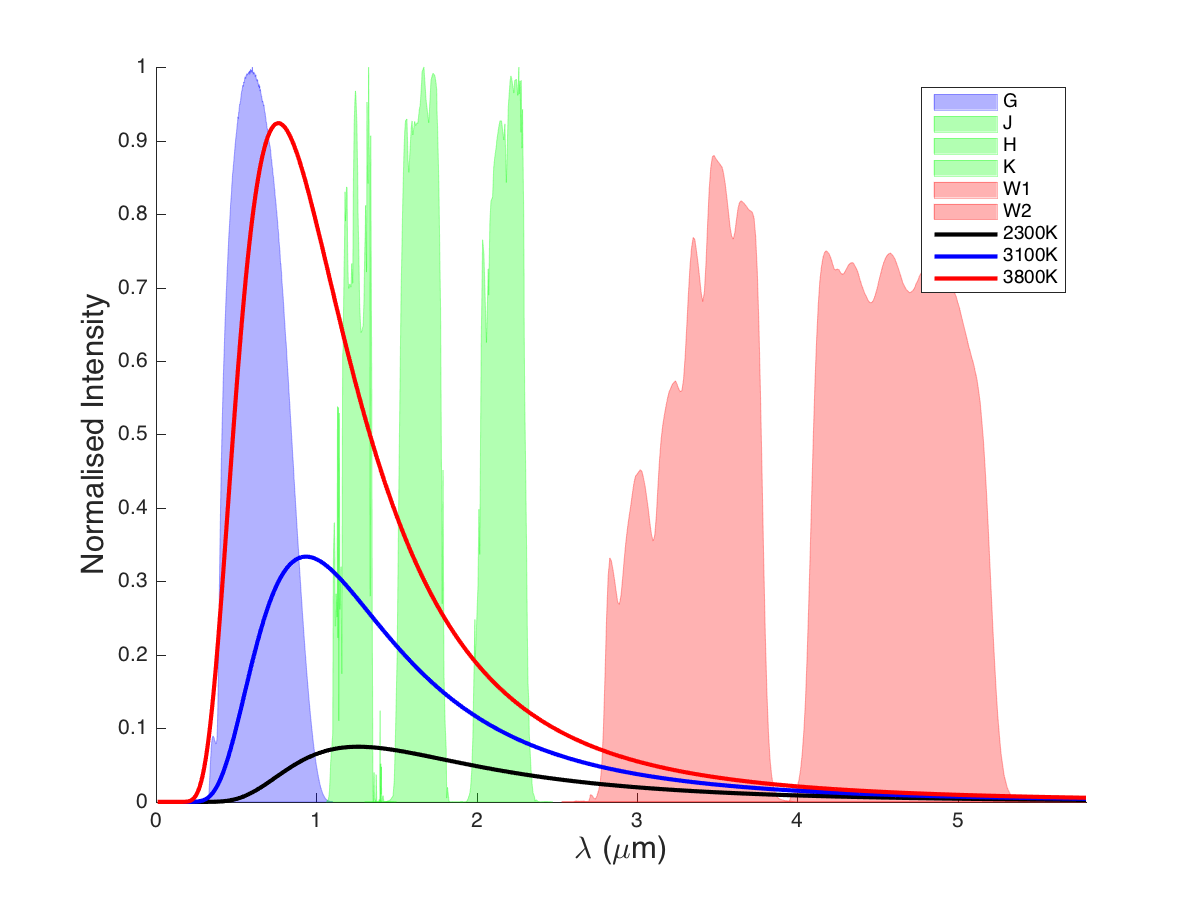
\includegraphics[width=0.8\textwidth]{Passbands.png}
    \caption{The wavelength coverage of the Gaia, 2MASS, and WISE photometry passbands. Overplotted is the blackbody curves of a M0 (red), M4 (blue) and M9 (black) star.}
    \label{figPassband}
\end{figure}

Using the {\em Gaia} archive\footnote{http://gea.esac.esa.int/archive/}, a working dataset of all objects from {\em Gaia} DR2 \citep{2018GaiaDR2} with G\,$<$\,14.5 was selected. These objects were also cross-matched against the 2MASS PSC and {\em WISE} AllWISE catalogues using their respective ``best neighbour'' cross match tables which use position and proper motion to match external catalogues to {\em Gaia} (see \citealt{2017Marrese} for full details). Additionally, the area of sky selected was limited to that accessible from the southern hemisphere ($\delta$\,\textless\,+10\,\degree) and avoided the Galactic plane ($|$b$|>$10\,\degree) -- the latter criterion was adopted because the large WISE full-width-at-half-maximum ($\approx$\,6\,") makes it difficult to match, or rely on, its data in crowded fields. Any object flagged in the AllWISE catalogue as a galaxy (xscproc\,$\neq$\,null), an extended object (ext\_flg\,$\neq$\,0), as multiple objects (n\_2mass\,\textgreater\,1) or as objects with poor/contaminated photometry (cc\_flags\,$\neq$\,0000) was also removed. The resulting catalogue contains roughly 8 million stars at G\,\textless\,14.5. Of these 8 million stars, 107,743 have no 2MASS cross-match and 627,127 have no WISE cross-match. For each star, photometry was required from all three surveys. Due to this, 638,845 stars were removed due to lack of cross-matches. This means that of all the observable stars with the requirements mentioned above, roughly 8\% will be missing from the sample.
\subsection{Spectroscopic comparison sample}
\label{secSpecData}
To provide a comparison set of photometry for stars with known spectral classifications, the same Gaia, 2MASS and WISE photometry was extracted for the large sample of M-dwarfs spectrally classified by \cite{2011West}, supplemented by the late K-dwarfs classified by \cite{2015Zhong}\footnote{While the Zhong K-dwarfs were useful for investigating the colour space where the K- and M-dwarfs intersect, the K7.5 stars were not included when determining the colour-subtype relationships (although their median colour values were included in Table 2.1 for completeness). The classification scheme used by \citealt{2015Zhong} is not the usual  Morgan–Keenan (MK) system, but is instead adapted from \citealt{2003Lepine}. While the K7 stars are classified using the Lepine system, their spectra should not differ significantly from the MK K7 spectral standard of 61 Cygni B and it is reasonable to include them in the analysis. The MK system does not recognise a K7.5 subtype and so they needed to be excluded.} This comparison sample consisted only of the stars that were quiescent for the passbands used in this work (var\_flg = XX\_\_, where X is from 0-5), and if the uncertainty in the {\em Gaia} parallax was less than, or equal to, 5\% of the parallax ($\sigma_\varpi/\varpi \leq 0.05$). Otherwise this comparison sample was selected in the same manner as the main sample. It should be noted that 99\% of these stars are dimmer than the G\,$<$\,14.5 magnitude limit of the main sample, however 54\% are within 229 pc, the magnitude limiting distance for observing M-dwarfs at G\,$<$\,14.5 (see Section\,\ref{secCombined}) and the photometric uncertainty was required to be 5\% or less of the magnitude. As such, the sample was not magnitude limited.\\

\begin{figure*}
	\centering
    \subfloat[]{\label{figRelGJ}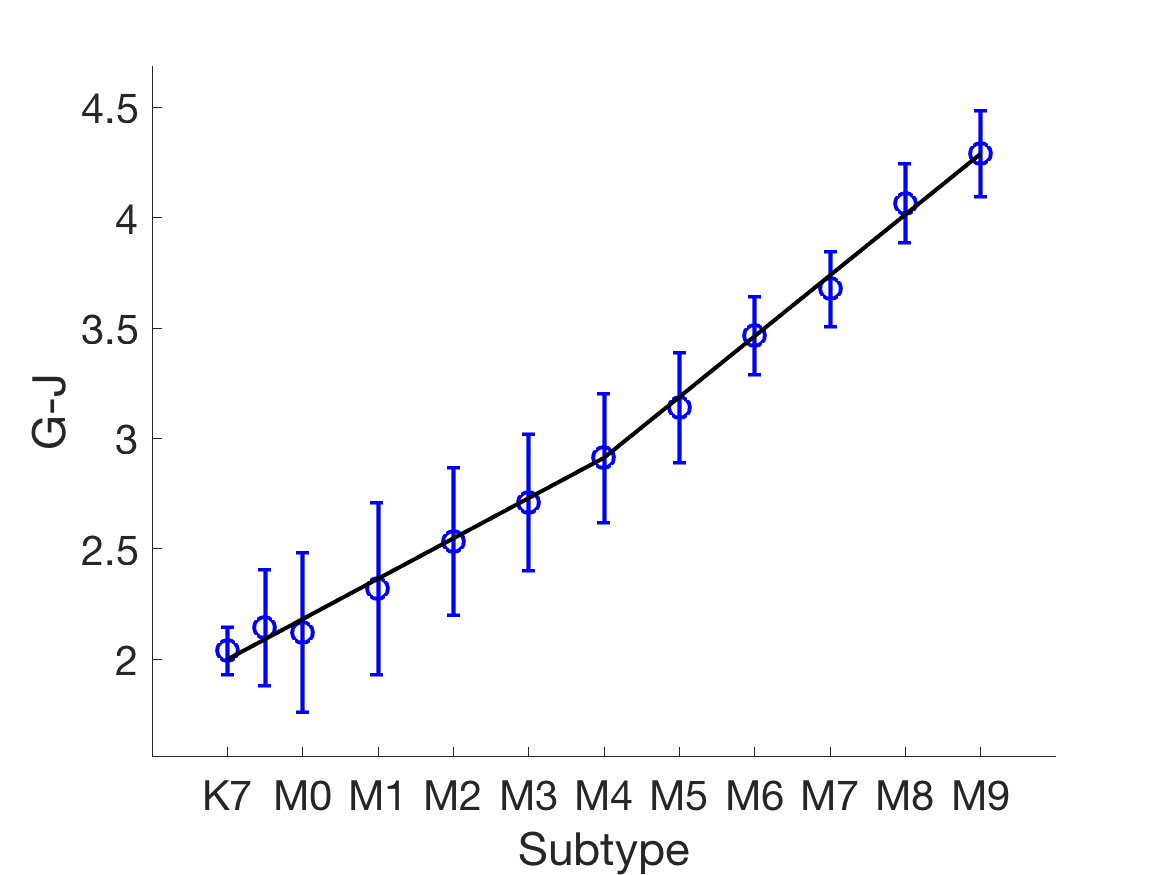
\includegraphics[width=0.5\textwidth]{RelationshipGJ.png}}
    \subfloat[]{\label{figRelGK}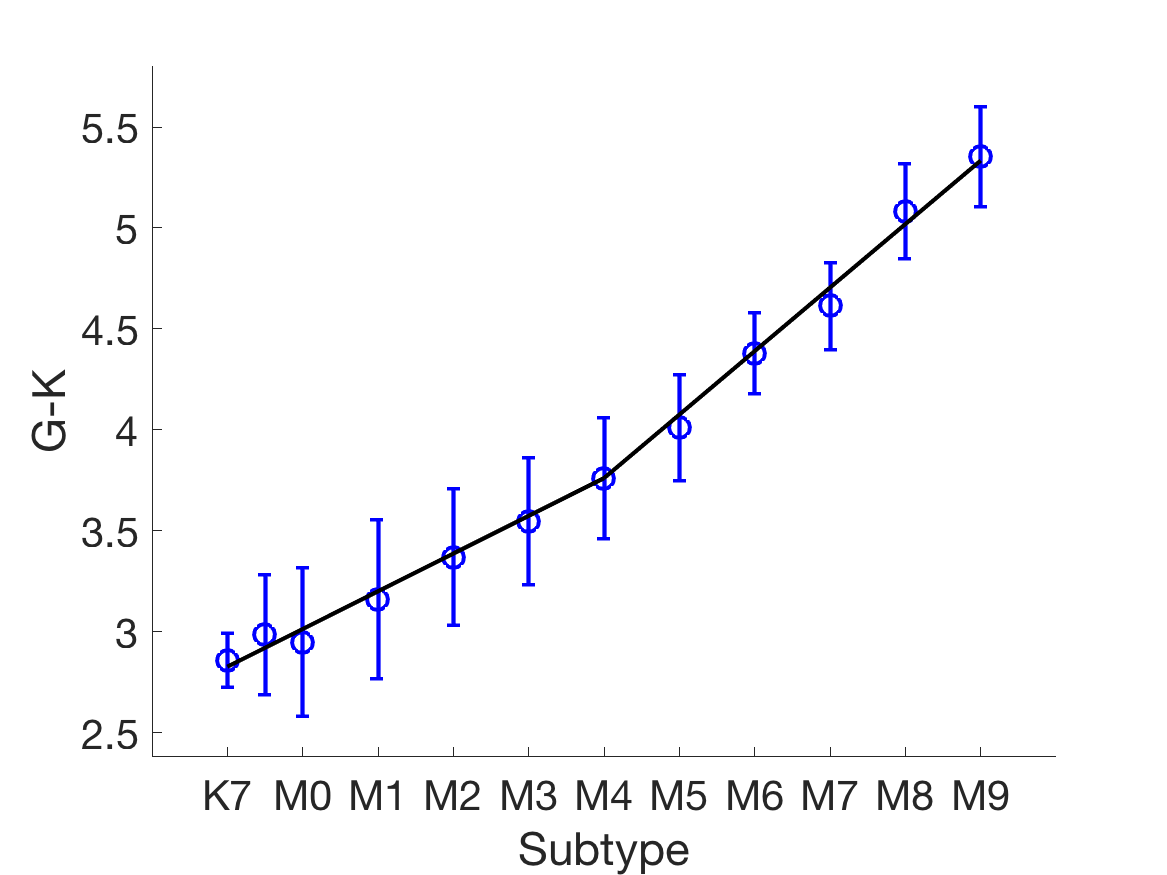
\includegraphics[width=0.5\textwidth]{RelationshipGK.png}}\\
    \subfloat[]{\label{figRelKW2}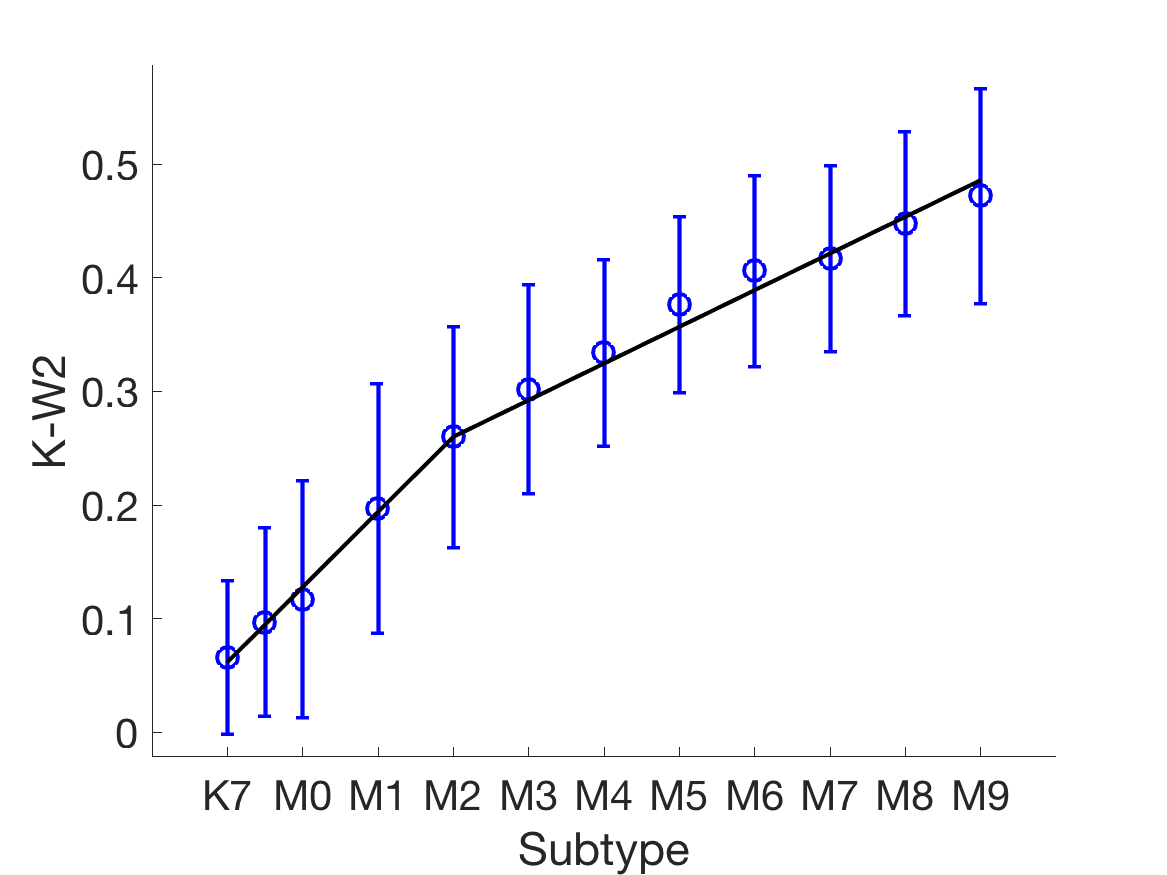
\includegraphics[width=0.5\textwidth]{RelationshipKW2.png}}
    \subfloat[]{\label{figRelW1W2}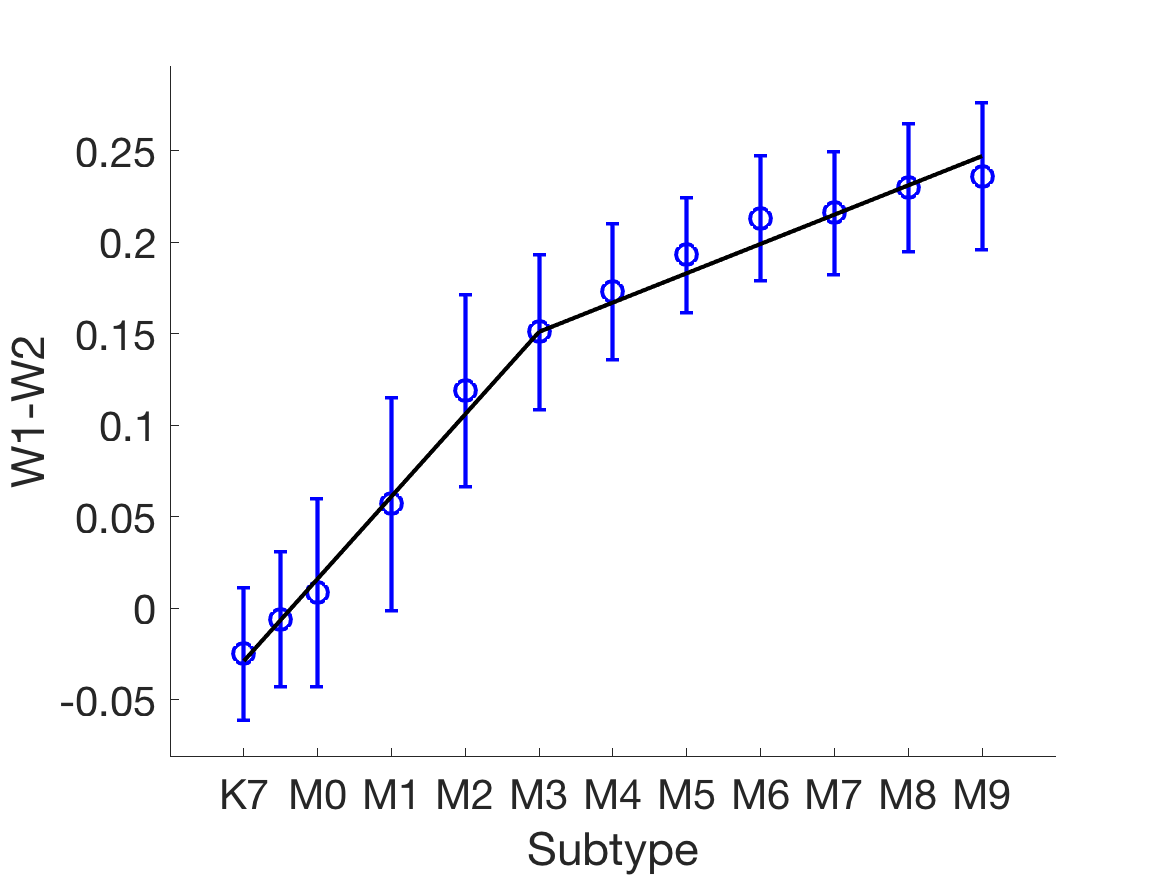
\includegraphics[width=0.5\textwidth]{RelationshipW1W2.png}}\\
    \subfloat[]{\label{figRelJK}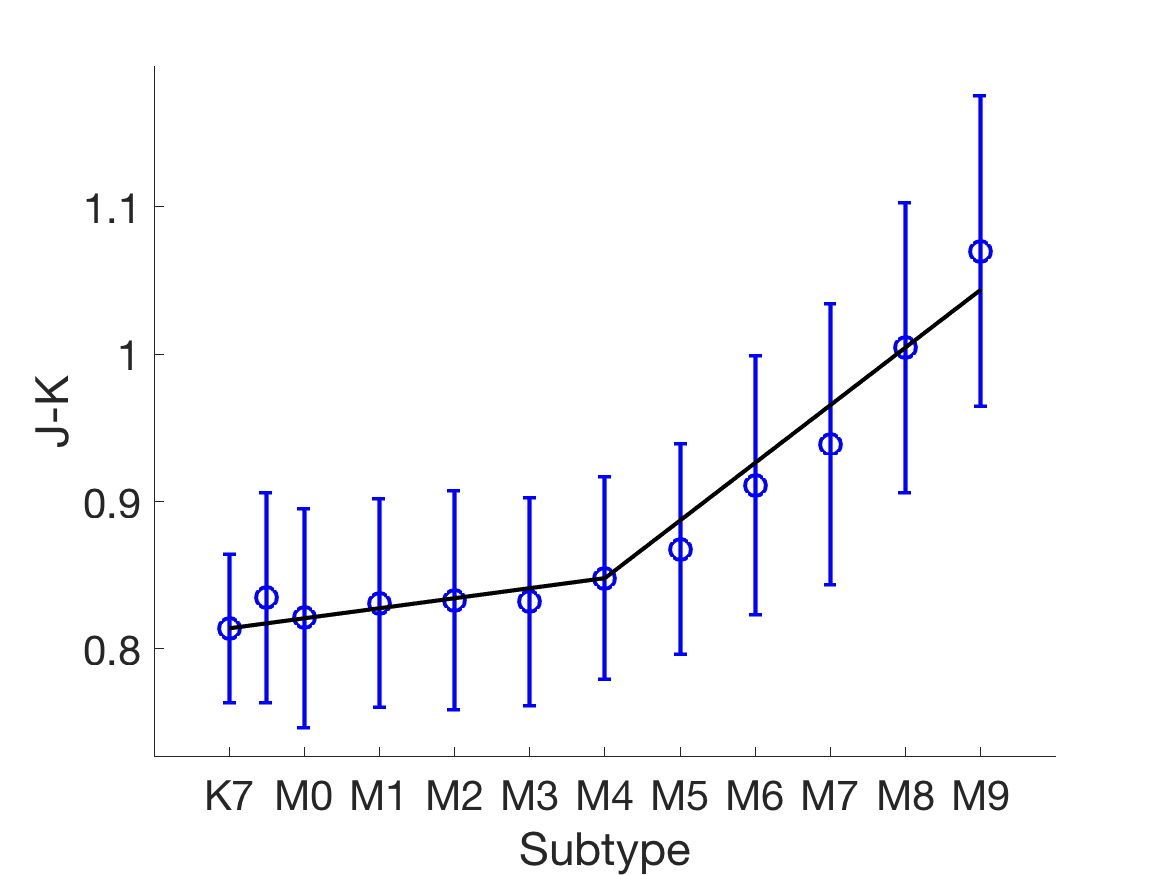
\includegraphics[width=0.5\textwidth]{RelationshipJK.png}}
    \caption{Photometric Gaia/2MASS/WISE colours as a function of spectral type for M-dwarfs of West et al. (2011) and late K-dwarfs of Zhong et al. (2015). Circles are the median colour values for each subtype, with uncertainty bars showing r.m.s scatter. The solid black lines are linear fits to the median subtypes. The outlier K7.5 median colour value for J--K was excluded when determining that parameterisation.}
	\label{FigRelationship}
\end{figure*}

Median colours were calculated and the r.m.s. scatter about the mean for each \citealt{2011West} defined spectral type, along with linear parametrisations of the median colours. The results of these parametrisations can be seen in Figure\,\ref{FigRelationship} for multiple colours and are tabulated in Table\,\ref{TabLookup} as a function of spectral type. In general the photometric scatter around these linear relationships are large - usually several tenths of a magnitude - with the scatter for optical-infrared colours becoming as large as seven-tenths of a magnitude at early types. This is much larger than expected due to the photometric measurement uncertainty of these surveys, suggesting this scatter is dominated by cosmic scatter due to metallicity variations, age variations, unresolved binarity, etc. Nonetheless, the trends with spectral type are consistent and smoothly varying\footnote{From the figures, it is clear that the parameterisation for each colour is represented by two linear relationships. The slope of the relationships, and the subtype at which one relationship changes to the second, varies with colour. Unlike the majority of the colours where the rate of change in colour increases with later subtypes, those with one, or both, of the WISE passbands display a lower rate of change. This may be due to the lower levels of flux across the WISE bands (see Figure\,\ref{figPassband}).} Figure\,\ref{figSubtypes} shows the spectral type distribution for J--W1/W1--W2, overplotted on a synthetic population (see Section\,\ref{secModel}).

\begin{table*}
	\begin{tabular}{| l | c | c  c | c c | c c | c c | l |}
	\hline
	Type & N  & G--J & r.m.s. & G--K & r.m.s. & K--W2 & r.m.s. & W1--W2 & r.m.s. & Src\\
	\hline
	K7 & 211 & 1.999 & 0.302 & 2.826 & 0.309 & 0.062 & 0.09 & -0.029 & 0.046 & ZJ \\
	K7.5 & 153 & 2.091 & 0.296 & 2.92 & 0.305 & 0.095 & 0.09 & -0.006 & 0.046 & ZJ \\
	M0 & 1160 & 2.182 & 0.291 & 3.013 & 0.302 & 0.128 & 0.09 & 0.016 & 0.045 & WA \\
	M1 & 1127 & 2.364 & 0.28 & 3.2 & 0.294 & 0.194 & 0.089 & 0.061 & 0.044 & WA \\
	M2 & 1999 & 2.547 & 0.269 & 3.387 & 0.287 & 0.26 & 0.089 & 0.106 & 0.043 & WA \\
	M3 & 2948 & 2.73 & 0.259 & 3.574 & 0.28 & 0.292 & 0.088 & 0.151 & 0.042 & WA \\
	M4 & 2608 & 2.912 & 0.248 & 3.761 & 0.273 & 0.325 & 0.088 & 0.167 & 0.04 & WA \\
	M5 & 1162 & 3.188 & 0.237 & 4.075 & 0.266 & 0.357 & 0.087 & 0.183 & 0.039 & WA \\
	M6 & 1355 & 3.463 & 0.227 & 4.39 & 0.259 & 0.389 & 0.087 & 0.199 & 0.038 & WA \\
	M7 & 1240 & 3.739 & 0.216 & 4.705 & 0.251 & 0.421 & 0.086 & 0.215 & 0.037 & WA \\
	M8 & 418 & 4.014 & 0.205 & 5.019 & 0.244 & 0.454 & 0.086 & 0.231 & 0.036 & WA \\
    M9 & 231 & 4.29 & 0.195 & 5.334 & 0.237 & 0.486 & 0.085 & 0.247 & 0.034 & WA \\
	\hline
	\end{tabular}
    \caption{Colour sequences (and r.m.s. scatter about them) for late-K- and M-dwarfs. Spectral type sources are: ZJ, Zhong et al. (2015); WA, West et al. (2011).}
    \label{TabLookup}
\end{table*}
\section{Simulations}
\label{secModel}
To test colour-based selection criteria,  simulated photometry of a synthetic population of stars was created using {\em Galaxia} \citep{2011Sharma}. This is a Galactic simulation code that generates a synthetic stellar population, including parameters for every star simulated such as their masses, ages, temperatures and simulated photometry. {\em Galaxia} generates its synthetic populations based on models for the Galaxy's stellar populations and its star formation history. It first generates a population with a set of basic physical parameters (position, distance, mass, age, metallicity) very similar to the Besan\c{c}on model \citep{2003Robin}  to generate the thin disc, the thick disc, the bulge and the halo populations (respectively). It then derives the resulting luminosity, effective temperature, photometric magnitudes and colours for each star, using the PARSEC-v1.2S isochrones \citep{2012Bressan, 2014Tang, 2014Chen, 2015Chen}, the NBC version of bolometric corrections \citep{2014Chen}, and assuming Reimers mass loss with efficiency $\eta=0.2$ for RGB stars. This photometry then has corrections applied to simulate the effects of extinction \citep{2011Sharma}. These simulations therefore include the effects of cosmic scatter due to metallicity variation and extinction, but do not include photometric measurement scatter, or the effects of source confusion. The simulation generated for this work was initially created for a magnitude limit of G\,\textless\,16, so that it would remain complete to G\,=\,14.5 when subject to the impacts of extinction and photometric scatter.\\

Because the {\em Galaxia} population is generated based on physical parameters,  relationships between those parameters (i.e. mass, radius, gravity, age, temperature) and the predicted spectral types of interest needed to be determined. In particular, what gravities and effective temperatures correspond to M-dwarfs? The temperature and gravity estimates of Table 4.1 from \citet{2005Reid} were adopted in this work -- specifically a {\em Galaxia} object is considered an M-dwarf if it has 2250\,K\,\textless\,T\,\textless\,3900\,K and 4.2\,\textless\,$\log g$\,\textless\,5.4. Any object younger than 500\,Myr was not considered an M-dwarf for this work. This, plus estimates for K-dwarfs, M- and K-giants, are presented in Table\,\ref{TabMK}. The M-dwarf classification identifies $\approx$\,20,000 stars as M-dwarfs within the G\,\textless\,14.5 {\em Galaxia} sample of $\approx$\,4.9 million stars.\\

\begin{table}
\begin{center}
	\begin{tabular}{| c | c | c | c |}
		\hline
        Sp. Type & log(g) & Age\,(Yr) & T\,(K) \\
        \hline
        M-dwarf & 4.2\,-\,5.4 & \textgreater\,5\,x\,10$^{8}$ & 2250\,-\,3900 \\
        K-dwarf & 4.2\,-\,5.4 & \textgreater\,5\,x\,10$^{8}$ & 3900\,-\,4600 \\
        M-giant & \textless\,4.2 & \textgreater\,5\,x\,10$^{8}$ & 2250\,-\,3900 \\
        K-giant & \textless\,4.2 & \textgreater\,5\,x\,10$^{8}$ & 3900\,-\,4600 \\
        \hline
\end{tabular}
\caption{Stellar characteristics used to define the M and K, dwarf and giant populations in the synthetic {\em Galaxia} population.}
\label{TabMK}
\end{center}
\end{table}
Figure\,\ref{figScatterB} shows a density plot of this {\em Galaxia} sample in the J--W1/W1-W2 plane, along with the objects identified as M-dwarfs by the adopted criterion (over-plotted in red).\\

{\em Galaxia} is necessarily limited in its predictive power for the photometry of sources by its PARSEC stellar models. In particular, {\em Galaxia} cannot predict the photometric properties of the latest M-dwarfs, because they are not included in the PARSEC isochrones. Specifically there are no isochrones for dwarfs of later than M5 (i.e. for T\,\textless\,2700\,K with 4.2 $<$ $\log g$ $<$ 5.4). This is highlighted in Figure\,\ref{figSubtypes} an expanded region of Figure \ref{figScatterB} around the M-dwarf branch, along with the M-dwarf sequence for spectroscopically observed M-dwarfs from Section\,\ref{secSpecData}. The latest spectroscopically observed M-dwarfs (M6-9 plotted in blue) lie in a region where {\em Galaxia} simulates almost no objects, because it {\em can} simulate no objects.\\

\begin{figure}[!ht]
    \centering
    \subfloat[]{\label{figScatterA}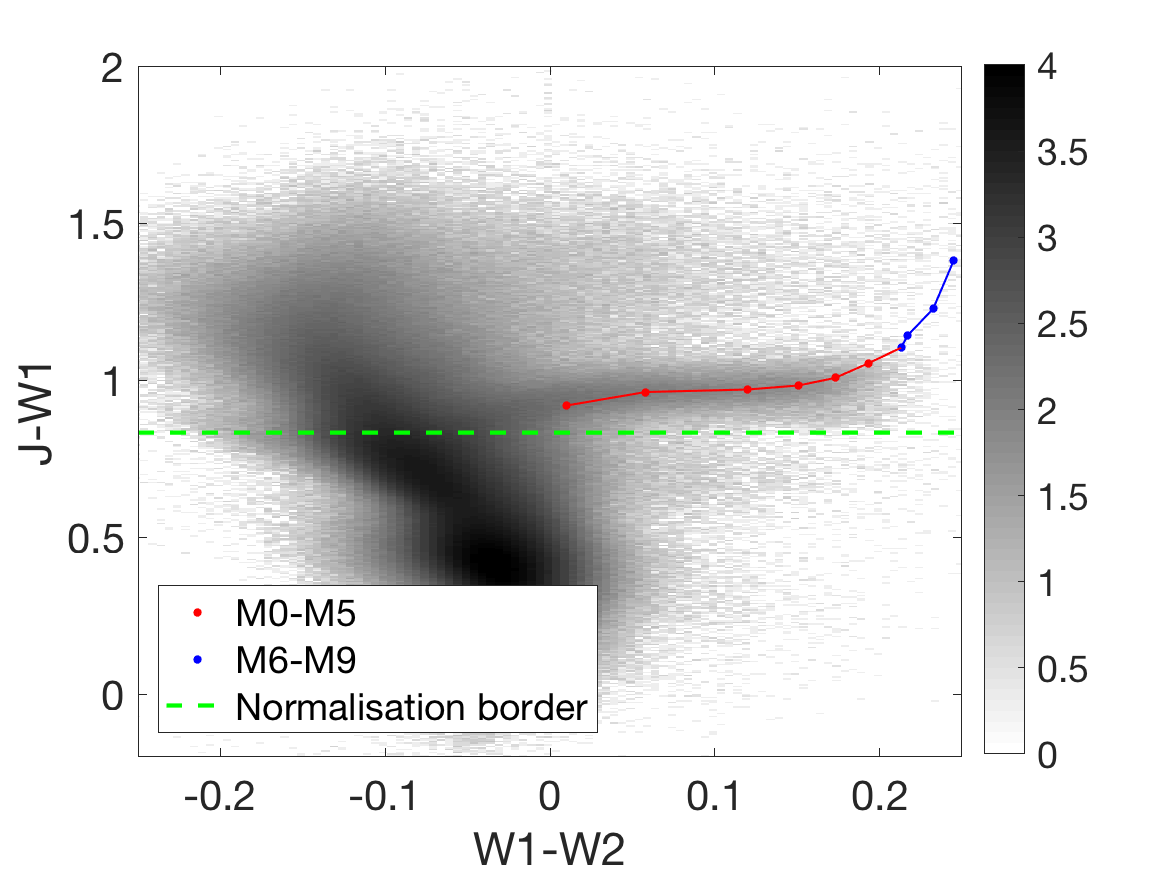
\includegraphics[width=0.8\textwidth]{MDwise.png}}\\
    \subfloat[]{\label{figScatterB}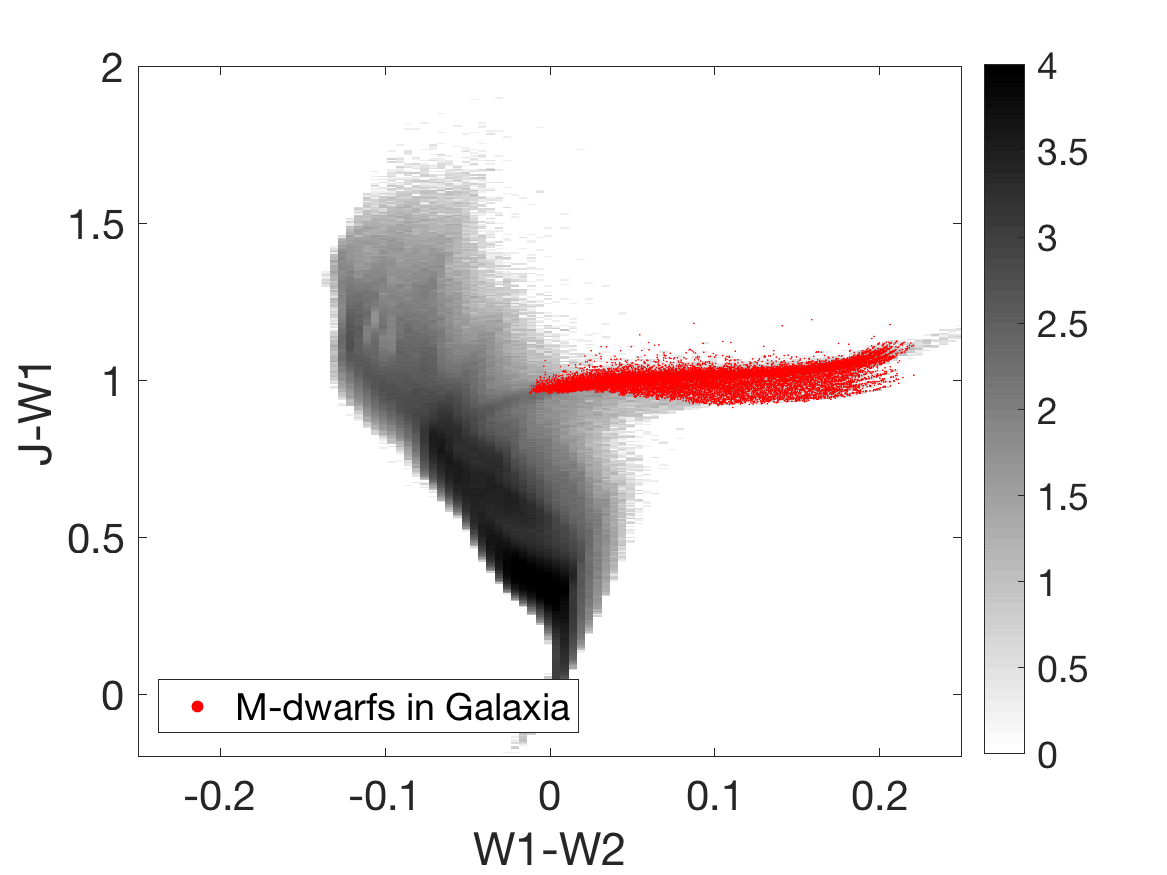
\includegraphics[width=0.8\textwidth]{MDgalaxia.png}}
    \caption{Logarithmic source densities in the J--W1/W1--W2 plane for sources with 9\,\textless\,G\,\textless\,14.5. Figure\,\ref{figScatterA} shows the {\em Gaia}/WISE/2MASS data. Objects below the green horizontal line in the  are used to normalise {\em Galaxia} to observational data, and the M-dwarf spectroscopic comparison sample from Section\,\ref{secSpecData} are overplotted in red and blue. Figure\,\ref{figScatterB} shows the {\em Galaxia} synthetic star population including cosmic scatter and extinction, but without photometric measurement scattering. M-dwarfs (see text) are highlighted in red.} 
    \label{figScatter}
\end{figure}
However, it should be noted that:
\begin{itemize}
	\item The number of M dwarfs will drop dramatically at later spectral types in any magnitude limited sample.
	\item These late M-dwarfs have photometric properties that are well-known from other work \citep{2002Leggett} and Section\,\ref{secSpecData} making them quite easy to distinguish from M-giants and other types of stars\,\citep{2011Lepine}.
	\item The TESS survey (at least) will focus on M-dwarfs earlier than M5 \citep{2015Ricker}.
\end{itemize}
As a result these ``missing'' {\em Galaxia} late M-dwarfs will make an insignificant contribution to estimates of completeness and contamination.\\

\begin{figure}[!ht]
	\centering
	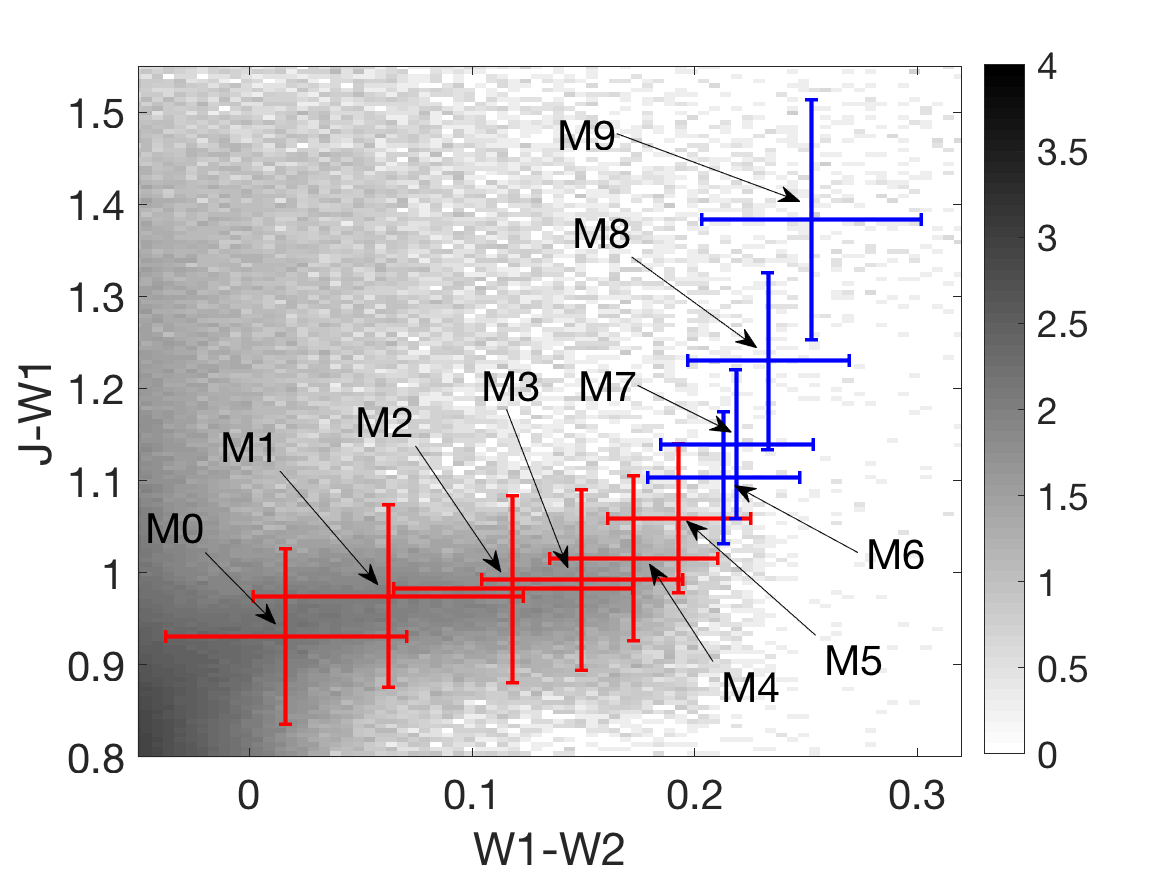
\includegraphics[width=0.8\textwidth]{Subtypes-2.png}
    \caption{{\em Galaxia} generated colour-colour density in J--W1/W1--W2 expanded around the M-dwarf branch. Overplotted are points representing the median colour and r.m.s. for spectroscopically observed M-dwarfs (M0-M5 in red, M6-M9 in blue).}
    \label{figSubtypes}
\end{figure}
\subsection{Photometric scatter}
\label{Scattering}
As noted above, scatter needs to be added to  {\em Galaxia}'s simulated photometry to match the expected photometric uncertainties for the observational data -- this is obvious from Figs. \ref{figScatterA} and \ref{figScatterB}, where it can be seen that the observed distribution is noticeably more scattered from the {\em Galaxia} one.\\

The observational data all come with estimated 1-$\sigma$ uncertainties, so uncertainty distribution functions were obtained for each observed bandpass by binning these uncertainties in 0.005 magnitude bins (for 2MASS/WISE) and 0.0002 magnitude bins (for {\em Gaia}) -- see Figure\,\ref{figDelta} for an example. \\

For each simulated magnitude (e.g. $W1$), a random draw was obtained from the appropriate distribution function for that magnitude bin, to obtain an estimate of the uncertainty for that simulated object (e.g. $\sigma_{W1}$). A second random draw was obtained from a normal distribution scaled to the previously drawn uncertainty to obtain a scattering estimate (e.g. $\Delta_{W1}$), which was applied to the simulated magnitude to obtain a scattered magnitude. Following the application of this suitable level of photometric scatter, the simulation was then trimmed to only contain simulated sources with G\,\textless\,14.5.\\

\begin{figure}[!ht]
	\centering
    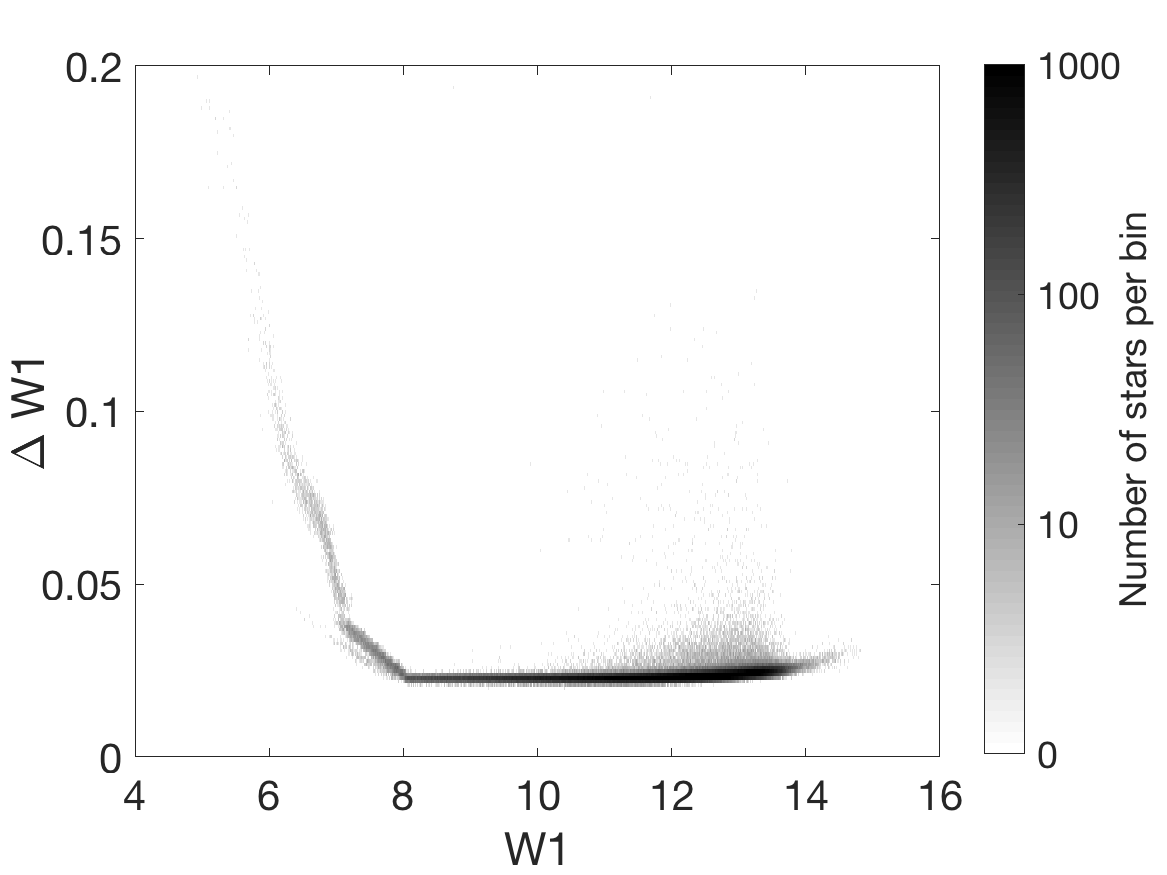
\includegraphics[width=0.8\textwidth]{deltaW1.pdf}
    \caption{Density plot of the number of stars per bin of the WISE photometric uncertainty as a function of the WISE magnitude W1.}
    \label{figDelta}
\end{figure}

The result of this photometric scattering applied to the data of Figure\,\ref{figScatterB} is shown in Figure\,\ref{figScatterC} -- the result is to significantly ``over scatter'' the simulated data compared to the observational data of Figure\,\ref{figScatterA}. All the features in W1--W2 in the scattered simulated data are too broad, as is the width of the M-dwarf branch in the J--W1 direction. The photometric confusion found in the observational data was more complex than just a simple normalised Gaussian distribution. It is expected that the photometric confusion seen is a product of multiple effects. At the very least, there is two levels of confusion in Figure\,\ref{figScatterA}. One that represents the minimally scattered, high-density population in the centre of the distribution, and the wider distribution of scattered stars that comprise the majority of what is seen in a colour-colour diagram (including the M-dwarf branch). \\ 

\begin{figure}[!ht]
    \centering
    \subfloat[]{\label{figScatterC}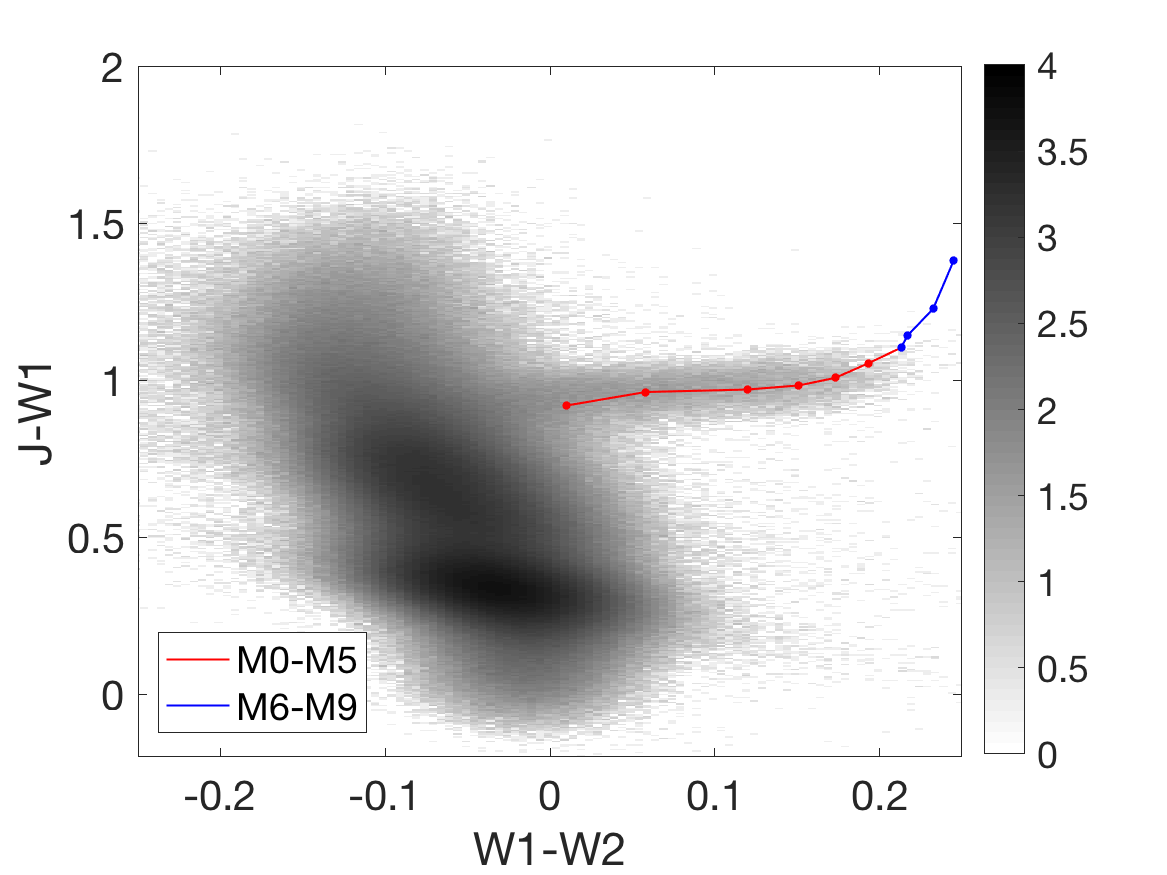
\includegraphics[width=0.8\textwidth]{Blur.png}}\\
    \subfloat[]{\label{figScatterD}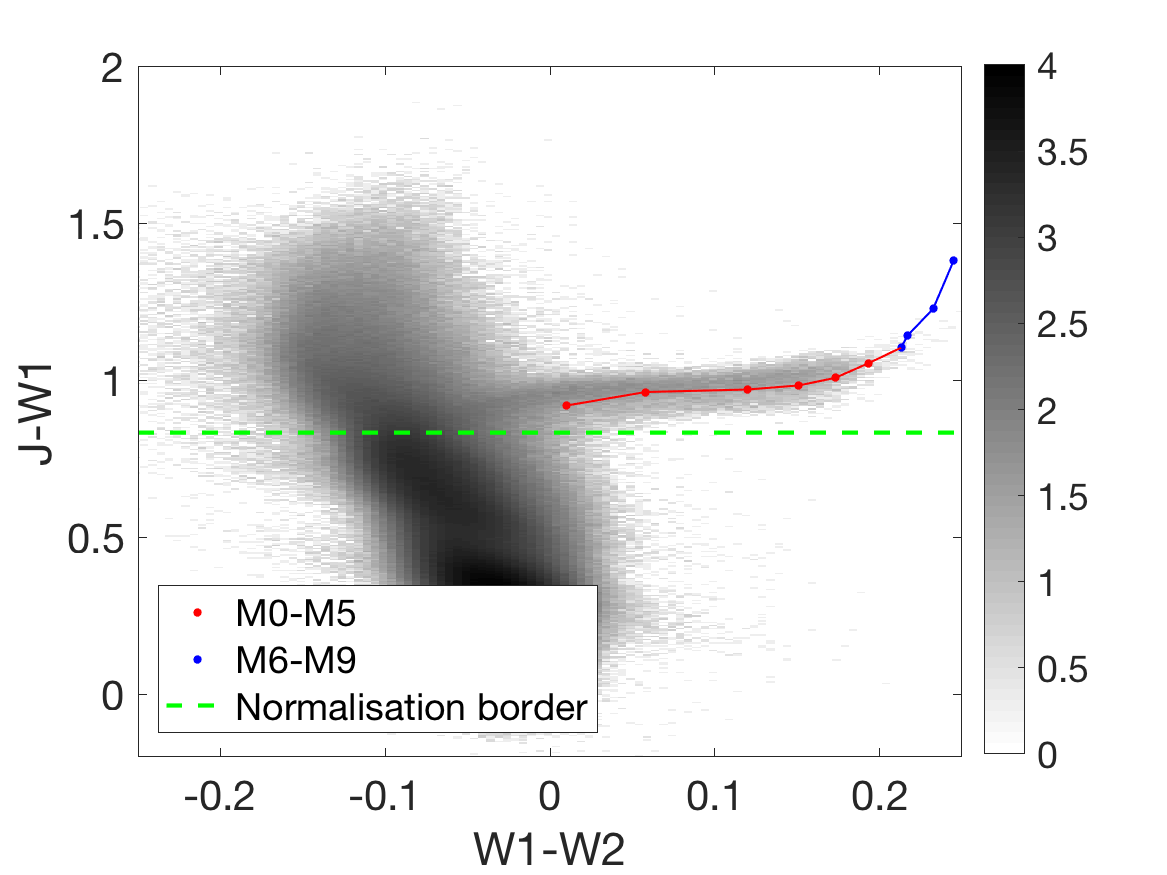
\includegraphics[width=0.8\textwidth]{galaxia.png}}
    \caption{Logarithmic source densities in the J--W1/W1--W2 plane for {\em Galaxia} data with two values of photometric scatter applied. Figure\,\ref{figScatterC} has the all the photometric scatter from the empirically determined relationships applied, while Figure\,\ref{figScatterD} has half of the scatter applied. Objects below the green horizontal line in Figure\,\ref{figScatterD} are used to normalise  {\em Galaxia} to observational data. The M-dwarf spectroscopic comparison sample from Section\,\ref{secSpecData} are overplotted in red and blue.} 
    \label{figPhotoScatter}
\end{figure}

As a response to this, two alternate methods were investigated. The first was to convolve the {\em Galaxia} colour data with a two dimensional kernel. This kernel was comprised of two, two dimensional Gaussians, which was hoped to simulate both populations mentioned above. This method has an added advantage over the previous method. The observational and synthetic datasets have different total populations. To accurately match the synthetic to the observational data, it needs to be scattered and normalised to match the observational. The level of scattering applied will also alter the amount that the synthetic population needs to be scaled by to match the observational data. This method determines both simultaneously as the kernel can scale the data it is convolved with. After empirically determining the lower and upper boundary conditions for each of the Gaussians comprising the kernel, a non-linear least-squares routine was applied to find the kernel that would produce a scattered synthetic population closest to the observation data by minimising the residuals between the two datasets. This resulted in a population significantly broadened, to the point that it no longer resembled the observational data at all. Visually determining the parameters needed for the kernel to scatter the {\em Galaxia} data produced data seen in Figure\,\ref{figKernel}.\\

\begin{figure}[!ht]
	\centering
    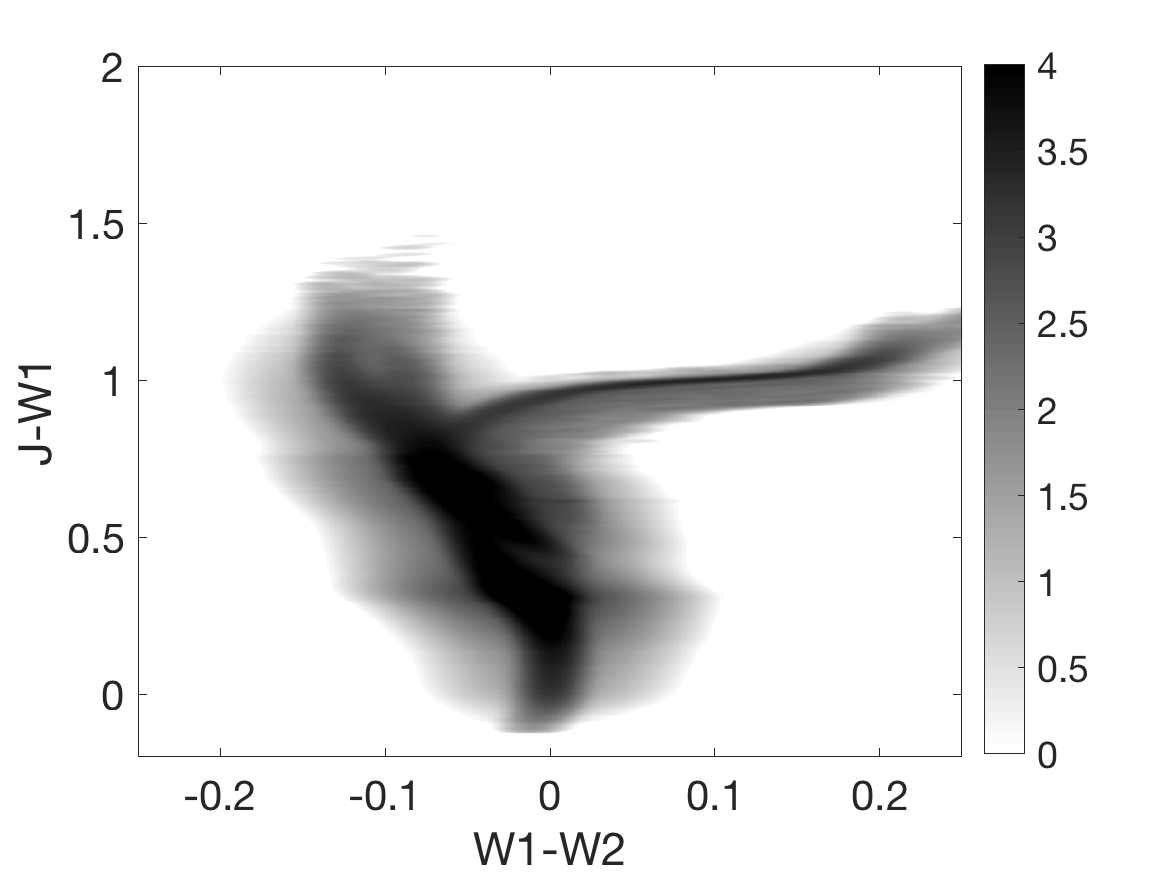
\includegraphics[width=0.8\textwidth]{Kernel.png}
    \caption{Density plot of the {\em Galaxia} dataset photometrically scattered by convolution with a 2-dimensional kernel.}
    \label{figKernel}
\end{figure}

The other method was to simply lower the fraction of the predicted photometric scatter applied to the simulated data. The amount required was empirically determined, so as to matched the observed distribution. It was found the initial scattering needed to be reduced by factors of near a half, and the resulting photometrically scattered data is shown in Figure\,\ref{figScatterD}.\\

Comparison of Figures\,\ref{figKernel} and \ref{figScatterD} show that while the kernel method does a better job of simulating the scale of both the populations mentioned above, it concentrates far too many stars in the high density regions, while the observational data shows a graduation between the two levels of scattering. The reduced photometric scatter method achieves a better simulated population in the regions that are most important - the high-density regions of hot stars and the M-dwarf branch, despite a lack of highly scattered stars at the ``edges''. Therefore the reduced photometric scatter method of Figure\,\ref{figScatterD} was used.
\subsection{Colour terms and offsets}
\label{secOff}
Comparison of the simulated and scattered data with the observational data, showed small -- but notable -- colour differences between {\em Galaxia} predicted colours and observed colours at the level of between several-hundredths to a few-tenths of a magnitude. This is not entirely surprising, inasmuch as the {\em Galaxia} predicted colours rely entirely on synthetic model atmospheres and model filter profiles. \\

``Benchmark'' features in the observed data were used to align the two sets of data. Figure\,\ref{figLandmark} shows example contours (rather than grey scales) of source density in J--W1/W1--W2 after these offsets were determined and applied. Offsets were determined using observed stars with G\,=\,9-14.5 from a number of features: the M-dwarf branch at J--W1$\approx$1; the G-dwarf clump at W1--W2\,$\approx$\,-0.03, J--W1\,$\approx$\,0.35; and the giant clump at W1--W2\,$\approx$\,-0.07, J--W1\,$\approx$\,0.7. As the aim of this work is to understand how selection criteria for M-dwarfs will be influenced by contamination, these offsets were weighted more heavily on the features nearest to the M-dwarf branch, as these are the source most likely to contaminate the M-dwarf selection. This is why in Figure\,\ref{figLandmark} the giant clump is better aligned than the G-dwarf clump. The offsets so determined and applied are reproduced in Table\,\ref{tabOffset}.\\

\begin{figure}
	\centering
    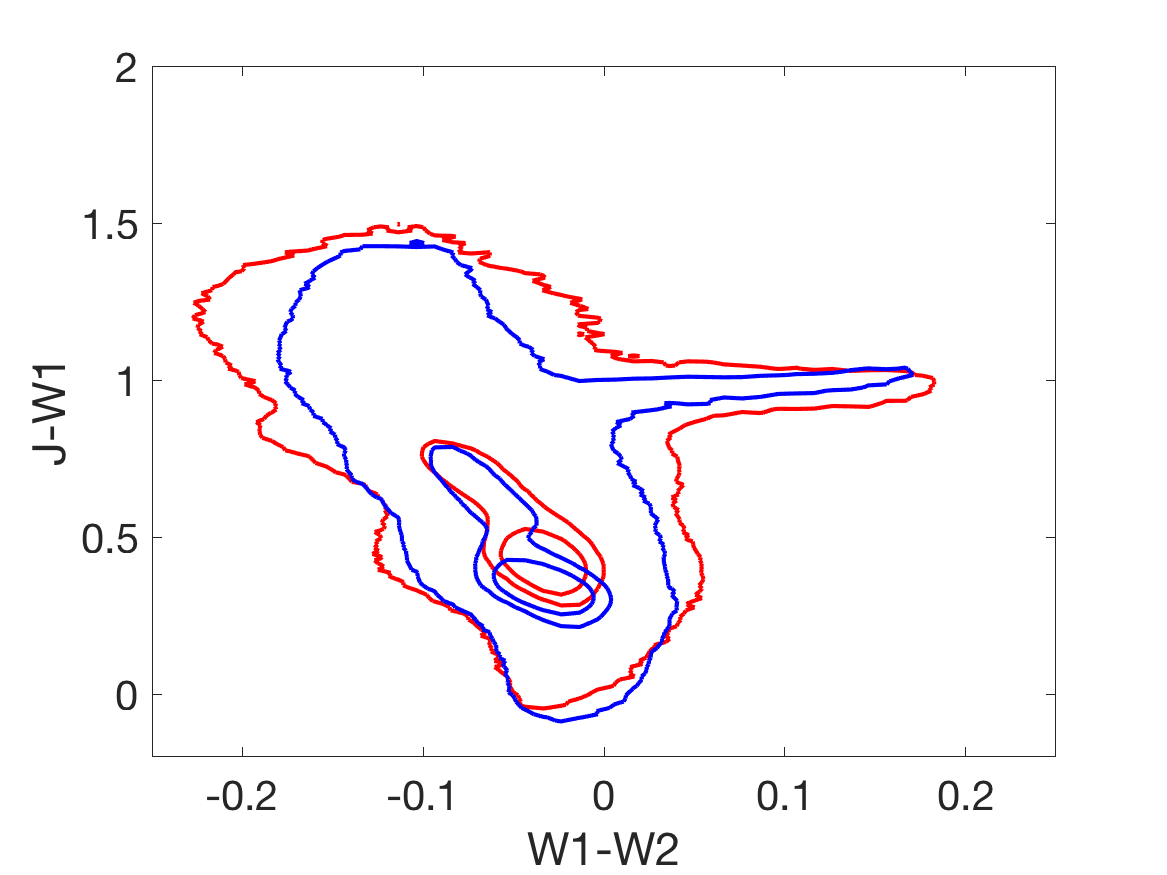
\includegraphics[width=0.8\textwidth]{Landmarks.pdf}
    \caption{Contours containing 30\%, 60\% and 99\% of the observational (in red) and simulated (in blue) data in J--W1, W1--W2. Offsets from Table\,\ref{tabOffset} have been used to align the simulation M-dwarf branch to its observational counterpart.}
    \label{figLandmark}
\end{figure}

\begin{table}
	\begin{center}
	\begin{tabular}{c c c c c} 
 		\hline
 		 G--J & G--H & G--K & G--W1 & G--W2\\
 		-0.01 & -0.02 & -0.05  & -0.05  & -0.1\\
        \hline
            & J--H & J--K & J--W1 & J--W2\\
            & -0.01 & -0.01 & -0.03 & -0.07\\
            \cline{2-5}
            \cline{2-5}
            &    & H--K & H--W1 & H--W2\\
            &    & 0 & -0.02 & -0.05\\
            \cline{3-5}
            \cline{3-5}
            &    &    & K--W1 & K--W2\\
            &    &    & -0.04 & -0.02\\
            \cline{4-5}
            \cline{4-5}
            &    &    &     & W1--W2\\
            &    &    &     & -0.025\\
 		\cline{5-5}
	\end{tabular}
    \caption{Zero-point colour offsets to align {\em Galaxia} colours with observed colours (in the sense that these offsets are added to synthetic colours).}
    \label{tabOffset}
	\end{center}
\end{table}

\subsection{Normalising {\em Galaxia} to the sky}
\label{secNorm}
Each {\em Galaxia} simulation run produces an arbitrary number of stars, (for this work, 4,931,764 were generated). To compare this synthetic {\em Galaxia} population with the observational {\em Gaia}/WISE/2MASS data, a normalisation between the two data sets was required. As noted above, while the colour offsets adopted (Table\,\ref{tabOffset}) aligned the M-dwarf branch, and features near that branch, in both datasets, there remain  a number of differences.\\

As noted above the G-dwarf clump does not align in Figure\,\ref{figLandmark}, even after the M-dwarf and giant clumps are aligned. This is believed to be due to limits on the reliability of the synthetic photometry adopted by {\em Galaxia}. Even after aligning for colour offsets there clearly remain higher-order colour terms.\\

Another difference between the observed and simulated data is seen in the M-giant region at J--W1$>$1 (see Figure\,\ref{figScatterA} and \ref{figScatterD}). The real galaxy produces a plume of objects with a wide distribution of colours, while {\em Galaxia} simulates a much narrower range. This is likely to be due to the significant variability and mass-loss present in this class of stars, resulting in intrinsic reddening and scattering in colour that is highly variable from source to source. In this region the simulated data also contains fewer stars than the observational data.\\

Given these differences it was felt that normalising {\em Galaxia} to the Galaxy using the total number of objects in both samples would not be the best way to proceed. Instead a normalisation determined from a comparison of the types of stars best represented in both datasets was used. {\em Galaxia} has been heavily tuned to match the observed Galaxy for relatively unreddened G-K dwarfs and giants. Therefore normalisation of the two samples was performed using the total number of stars 0.1\,mag below the M-dwarf branch in each colour-colour space (shown by the green horizontal lines in Figures\,\ref{figScatterA} and \ref{figScatterD}), and adopted a normalisation factor of 1.3918 to scale up the synthetic population to match the observational data. This means that, while the overall population will be close in number, specific regions may have differing numbers of stars.

\subsection{Connected component analysis}
\label{secCCA}
To identify the distribution of M-dwarfs and other key populations in both absolute magnitude and colour space, Connected Component Analysis (CCA; \citealt{1988Samet}) was used. CCA is a technique that identifies the pixels of a 2-dimensional image that comprise each component of the image. For this work, the images of interest are density images created by binning {\em Galaxia} simulated objects in colour-colour planes. Using this technique, groups of components that comprise the majority of the sample can be selected, excluding highly scattered components that comprise a small fraction of the total population but would inflate the selected region, adding significant numbers of stars not intended to be selected (i.e. non-M-dwarfs). For example, Figure\,\ref{figCCA} shows an example use of this technique for a density image of the adopted {\em Galaxia} M-dwarfs in the G--K/K--W2 colour-colour plane. The green contour is a rough measure of the region bound by all the {\em Galaxia} M-dwarfs while the red contour uses CCA to select 99.5\% of the M-dwarfs but excludes a number of the most photometrically scattered M-dwarfs. Losing 0.5\% of the M-dwarfs in the sample is an acceptable sacrifice to reduce the selected region and avoid as many non-M-dwarfs as possible.\\

Using the expected properties of M-dwarfs from \citet{2005Reid} (summarised in Table\,\ref{TabMK}) to identify {\em Galaxia} sources as M- or K-giants, or K-dwarfs (as well as the previously discussed criterion for M-dwarfs). CCA was used to identify regions that contain \textgreater\,97\% of each of these classes of object in the {\em Galaxia} simulations (see Figure\,\ref{figCCP}).\\

\begin{figure}
	\centering
    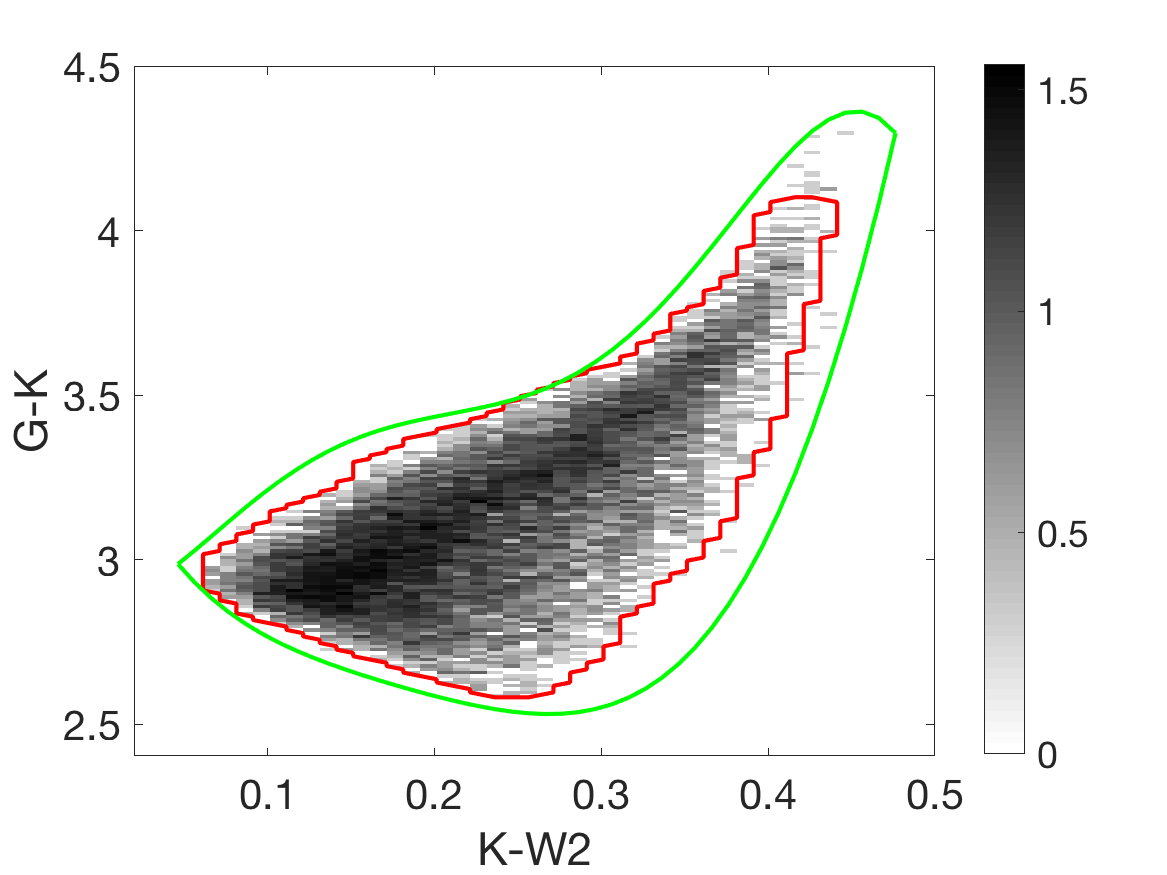
\includegraphics[width=0.8\textwidth]{CCA-2.pdf}
    \caption{Connected component analysis of the {\em Galaxia} M-dwarfs using the G--K and K--W2 colours. The red outline highlights the region defined as the largest component while the green line represents the boundary region around the entire {\em Galaxia} M-dwarf population for this colour plane.}
    \label{figCCA}
\end{figure}

\subsection{Completeness and contamination in simulations}
The simulated data allowed both the completeness and contamination (i.e. the false-positive rate) for each M-dwarf candidate selection method used, to be quantified. Simulated completeness is defined as the number of M-dwarfs selected, divided by the total number of M-dwarfs present in the simulation, and simulated contamination as the number of non-M-dwarfs identified by each set of criteria, divided by the total number of M-dwarfs and non-M-dwarfs selected by each set of criteria.
\section{Absolute Magnitude Selection}
\subsection{Selection criteria}
\label{secAbs}
Due to {\em Gaia} DR2's extensive catalogue of luminosities and distances, a primary selection of M-dwarfs via absolute magnitude is quite viable. Therefore, both the simulated data and spectroscopic comparison sample were used to examine the impact of a complete set of all-sky distance measurements.\\

A M$_G$/G--J colour-magnitude diagram was constructed using the simulated data (Figure\,\ref{figColMagA}), and the characteristics from Table\,\ref{TabMK}, plus CCA techniques, were used to identify and select the M and K dwarf, and M and K giant populations in this plane. It is clear that the risk of contamination of an M-dwarf sample by M and K giants is greatly diminished in absolute magnitude space, and the only significant issue in such a plane is the degree of K dwarf contamination as a function of an adopted upper luminosity limit in M$_G$ for M-dwarfs.\\

\begin{figure}
	\centering
    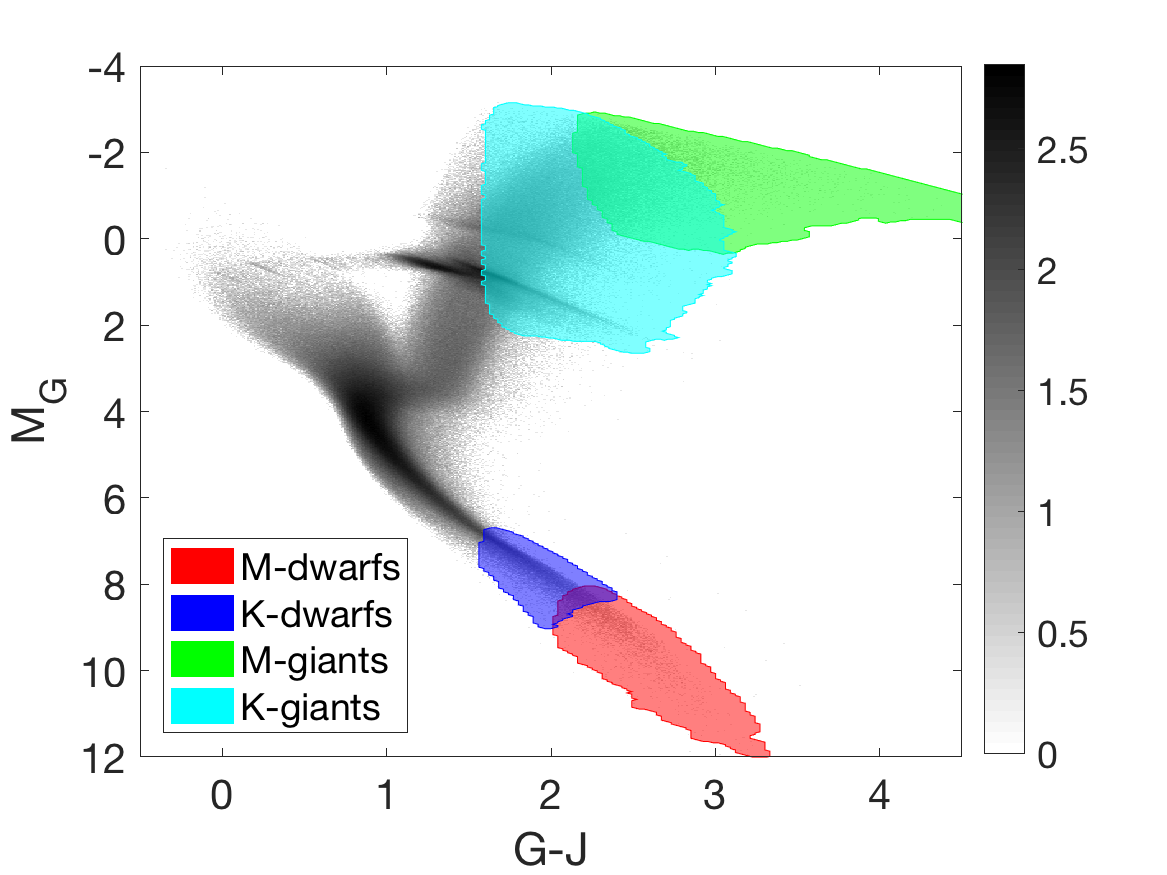
\includegraphics[width=0.8\textwidth]{AbsMag-G.png}
    \caption{Simulated M$_G$/G--J colour magnitude diagram for G\,\textless\,14.5. The K and M, dwarf and giant regions are identified using the criteria of Table\,\ref{TabMK}, and the overplotted CCA regions (complete to \textgreater\,97\%), where red is the simulated M-dwarfs, blue is the K-dwarfs, K-giants are in cyan, and M-giants are presented in green.}
    \label{figColMagA}
\end{figure}

Informed by these CCA regions, two M$_G$ cut-offs were chosen for M dwarf selection. An absolute magnitude limit of M$_G$\,\textgreater\,8.04, set at the bright end of the M-dwarf distribution, prioritising M-dwarf completeness, and a second limit which attempted to minimise K-dwarf contamination by setting the limit at M$_G$\,\textgreater\,8.86, the dim end of the K-dwarf distribution.\\

\begin{figure}
	\centering
	\captionsetup{width=.5\textwidth}
	\subfloat[A zoomed in image of the K to M dwarf boundary seen in Figure\,\ref{figColMagA}.]{\label{figColMagB}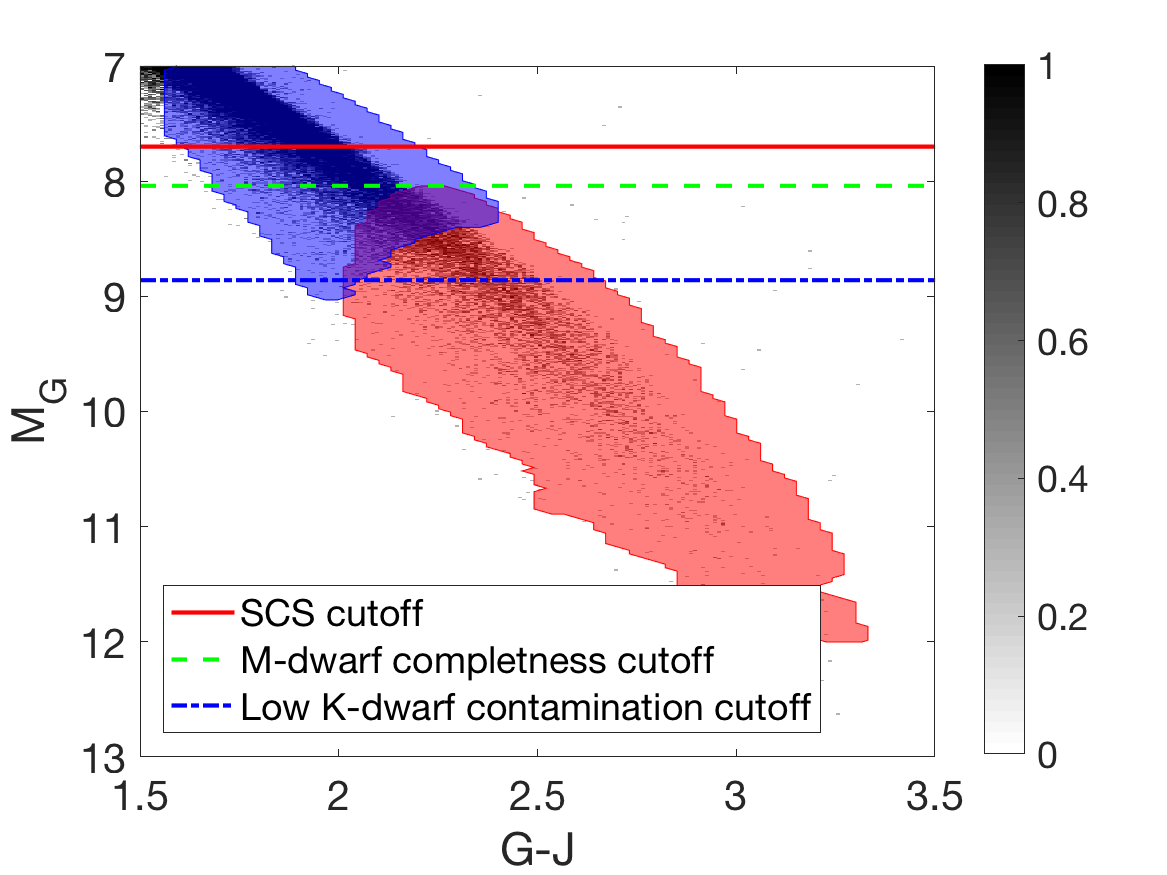
\includegraphics[width=0.6\textwidth]{MagCut_Close.png}}
	\subfloat[M$_G$/G--J colour magnitude diagram for the spectroscopic comparison sample.]{\label{figColMagC}\includegraphics[width=0.6\textwidth]{WestAbsMag.png}}
    \caption{}
    \label{figColMag}
\end{figure}

A similar test was conducted using the spectroscopic comparison sample, cross matched with {\em Gaia} to obtain G-band photometry and parallaxes (and therefore absolute magnitude). An absolute magnitude limit of M$_G$\,\textgreater\,7.70 is required to select 97\% of the comparison sample (shown by the red solid line in Figures\,\ref{figColMagB} and \ref{figColMagC}). Neither the external completeness, nor levels of contamination, can be determined for this sample, since the selection function of the spectroscopic comparison sample itself is not well determined, and it doesn't contain non-M-dwarfs to examine contamination.\\

All three of these absolute magnitude limits are presented in Figures\,\ref{figColMagB} and \ref{figColMagC} as the red (M$_G$\,\textgreater\,7.70), green (M$_G$\,\textgreater\,8.04), and blue (M$_G$\,\textgreater\,8.86) horizontal lines.\\

Absolute magnitudes for the simulated data were derived from the distances generated for each star in the simulated population. Distances for the observational data (and hence absolute magnitudes), were derived from the inverse of the parallax. For samples of the bright, nearby stars being considered (M$_G$\,\textgreater\,7.70, G\,\textless\,14.5 implies M-dwarfs will lie at a maximum distance of 229\,$\pm$\,2pc), the typical uncertainties in Gaia DR2 data mean that the biases arising from obtaining a distance from an inverted parallax are completely negligible. While it is known that Gaia DR2 contains a number of stars with parallaxes that are either negative, and/or un-physically large, the number of such objects at these bright magnitudes is very small\footnote{See \citealt{2018Luri} for details on the Gaia DR2 parallaxes}.
\subsection{Completeness}
Investigation of these limits (see Table\,\ref{tabAbs}) found that the M$_G$\,\textgreater\,8.86 selection would achieve an unacceptably poor level of completeness (54.8\%), so it was not considered further. The M$_G$\,\textgreater\,8.04 selection significantly reduced the contamination rate of non-M-dwarfs by a factor of about 2. Moreover it does so while maintaining M-dwarf completeness at 99.96\%.\\

\begin{table*}
\hspace{-5mm}
	\begin{tabular}{ | c | c c c c | c c |} 
		\hline
        & \multicolumn{4}{c|}{Simulations} & \multicolumn{2}{c|}{Observations}\\
		M$_G$ & Meet & Total & Completeness & Contamination & Meet & Total\\
        limit & Criteria & M-dwarfs & (\%) & (\%) & Criteria & M-dwarfs\\
		\hline
        \textgreater\,7.70 & - & - & - & - & 76392 & -\\
        \textgreater\,8.04 & 39435 & 27583 & 99.96 & 29.4 & 55230 & 38992\\
        \textgreater\,8.86 & 18347 & 15259 & 54.8 & 16.8 & 24853 & 11234\\
		\hline
	\end{tabular}
    \caption{Absolute magnitude M-dwarf selections determined from West et. al (M$_G$\,\textgreater\,7.7) and {\em Galaxia} (M$_G$\,\textgreater\,8.04 \& M$_G$\,\textgreater\,8.86).}
    \label{tabAbs}
\end{table*}
Applying the M$_G$\,\textgreater\,7.70 and M$_G$\,\textgreater\,8.04 limits to the observational absolute magnitudes selects 76,392 and 55,230 stars respectively. For the {\em Galaxia} derived M$_G$\,\textgreater\,8.04 limit, a significantly greater number of stars are selected from the observational data than the 39,435 stars predicted from the simulated data. It is believed to be due to the localised discrepancies between the simulated and observational data, mentioned in Section\,\ref{secNorm}.\\

M-dwarf selection via absolute magnitude requires a bright limit somewhere in the range 7.70\,-\,8.04. Adopting the more luminous of these limits (derived from the empirical spectroscopic comparison sample) results in a more complete sample of M-dwarfs, without selecting an unfeasibly large number of stars to observe with FunnelWeb (\textless\,100,000). Applying this conservative luminosity selected criterion (hereafter `AbsCrit') selects 76,392 stars. This absolute magnitude limit applied to {\em Galaxia} selects all of the stars determined to be M-dwarfs. From this, and the spectroscopic derived limit, the M-dwarf completeness of the AbsCrit criterion is estimated to be 96.98-100\%.
\section{Colour selection}
As a complimentary selection criteria, it was decided to use the long-standing tradition in giant-dwarf discrimination of selecting colour-colour diagrams which aim to break degeneracies between stellar effective temperature and surface gravity. Specifically, colours sensitive to effective temperature were found for the horizontal axes, and those sensitive to surface gravity for the vertical axes. Of course, no such diagram is perfect and contamination will occur where different classes of star overlap. Most notably for this case, the low-temperature boundary of the M-dwarf regime which adjoins the (much more numerous) high temperature boundary of the late K-dwarf regime, as well as the less numerous lower boundary of the K- and M-giants. Even small amounts of photometric scatter, cosmic scatter and source confusion in these more numerous populations will lead to significant contamination of any M-dwarf selection.
\subsection{Stellar distributions}
After examining the many colour-colour combinations available from the six passbands used in this work, three were selected for use in this analysis. They are presented in Figure\,\ref{figCCP}. Each possesses distinct advantages.\\

\begin{itemize}
\item{{\em G--K/K--W2}: This plane displays the smallest levels of K-dwarf/M-dwarf overlap in all the colour-colour planes. In all colour-colour planes, K-dwarfs are the most significant source of contamination in the M-dwarf region, so selecting a colour-colour space that minimises this overlap greatly lowers the overall level of contamination.}
\item{{\em J--K/G--J}:  This plane has the advantage of using the G-band in the temperature-dependent horizontal axis to distribute the M-dwarf branch across a large colour range.}
\item{{\em J--K/W1--W2}: This has the advantage of using a colour on the horizontal axis for which both bands come from the same survey, telescope and instrument, which reduces issues associated with cross-matching, and systematics between surveys with different sensitivities, instrument resolution and data processing.}
\end{itemize}

\begin{figure}
	\centering
	\vspace{-3cm}
    \includegraphics[height=0.35\textheight]{GKKW2.png}\\
    \includegraphics[height=0.35\textheight]{JKGJ.png}\\
    \includegraphics[height=0.35\textheight]{JKW1W2.png}\\
    \caption{The three colour-colour spaces chosen for this work. Coloured regions highlighting the four classes of stars of importance to this work, as identified by the CCA analysis described in Section\,\ref{secCCA}. In each case these connected regions contain \textgreater\,97\% of the relevant class in the {\em Galaxia} simulation. Red - M-dwarfs; Blue - K-dwarfs; Cyan - K-giants; Green - M-giants.}
    \label{figCCP}
\end{figure}
\subsection{Selection criteria}
Guided by the principle of keeping the photometric selection criteria as simple as possible. The initial work used simple rectangular selection regions in colour-colour space, bounded by the maxima and minima of the CCA regions for M-dwarfs. However, these were quickly found to be unsatisfactory -- there was simply too much contamination at the boundaries between between classes of object, which do not follow either vertical or horizontal lines in these planes.\\

\begin{figure}
	\centering
    \includegraphics[width=1\textwidth]{Parallelogram.pdf}
    \caption{Construction of a parallelogram selection region using the CCA information seen in Figure\,\ref{figCCA}. The red line bounds the primary connected component, the blue crosses represent the G-K values of highest density for the middle 60\% of the K-W2 bins. The thin green line is a linear fit through the blue crosses and the thick green lines represent the parallelogram formed from the intersection of the polynomial with the minimum and maximum K--W2 values from the primary connected component.}
    \label{figPara}
\end{figure}

The next simplest model (i.e. parallelograms) were utilised as the simplest polygon able to represent the M-dwarf region. The data in the M-dwarf CCA region was binned along each horizontal axis and fitted a linear polynomial to the middle 60\% of points in each bin. Figure\,\ref{figPara} shows an example of this for the data plotted in Figure\,\ref{figCCA}.\\

\begin{table}[]
    \centering
    \begin{tabular}{|r|}
        \hline
        High completeness criteria\\
        \hline
        K-W2\,\textgreater\,0.061\\
        K-W2\,\textless\,0.441\\
        G-K\,\textgreater\,3.26(K-W2)\,+\,2.124\\
        G-K\,\textless\,3.26(K-W2)\,+\,3.209
        G-J\,\textgreater\,2.011\\
        G-J\,\textless\,3.441\\
        J-K\,\textgreater\,-0.010(G-J)\,+\,0.723\\
        J-K\,\textless\,-0.010(G-J)\,+\,0.927
	    W1-W2\,\textgreater\,-0.059\\
        W1-W2\,\textless\,0.221\\
        J-K\,\textgreater\,-0.051(W1-W2)\,+\,0.720\\
        J-K\,\textless -0.051(W1-W2)\,+\,0.938\\
        \hline
    \end{tabular}
    \caption{Colour selection comprising the `high completeness' criteria.}
    \label{eqHC}
\end{table}

This results in the three groups of ``high completeness'' criteria shown in Table \ref{eqHC}, which are shown in Figure\,\ref{figBox} overplotted on the observational data as by the red parallelograms. Looking at the numbers selected by each criterion (Table\,\ref{TabColSelect}) two conclusions can be reached.\\

\begin{table*}
\begin{center}
	\begin{tabular}{| c | c | c | c || c | c | c || c |}
		\hline
        Data & A & B & C & A \& B & A \& C & B \& C & A \& B \& C\\
        \hline
        Simulated & 109310 & 193384 & 129136 & 66186 & 73507 & 67248 & 58264 \\
        Observational & 245736 & 329228 & 223686 & 108238 & 124243 & 121205 & 94145 \\
        \hline
\end{tabular}
\caption{Comparison of the number of stars selected from each colour criterion comprising Table\ref{eqHC}. `A' represents the G--K/K--W2 criterion; `B' is the J--K/G--J criterion and `C' is the J--K/W1-W2 criterion.}
\label{TabColSelect}
\end{center}
\end{table*}
Firstly, the J--K/G--J colour plane (B) selects significantly more stars than the other two colour regions. However, the combination of this colour criterion with either of the other two criteria (A \& B or B \& C) selects fewer stars than the combination without it (A \& C). The combination of all three reduces the number of selected stars even further, to just 60\% of the smallest colour selection (A). As stated previously, photometric confusion limits the ability to use a single colour range to define a single class of star. However, a contaminant in one colour is not necessarily going to be present as a contaminant in other colours. Selecting M-dwarfs via multiple colours and requiring a candidate star to fall within all of the M-dwarf colour ranges will reduce the number of contaminants selected. At the same time, selection by too many colour ranges might throw out a non-trivial number of M-dwarfs, lowering M-dwarf completeness. It was decided that three colour-colour planes would be a reasonable balance.\\

It was then made a requirement that an object must satisfy all three of these colour-colour criteria to be considered a candidate M-dwarf. Secondly, the total number of stars within the simulated colour regions are much less than the corresponding regions in the observational data. Of particular note is the B \& C combination, in which the simulated numbers are, at worst, 9\% smaller than the other combinations, while the observational population is roughly 50\% greater than the other populations. This was expected (see Section\,\ref{secNorm}), however this highlights the extent to which specific regions might differ between the simulated and observational datasets.\\

\begin{figure}
	\centering
	\vspace{-3cm}
    \subfloat[]{\label{figBoxA}\includegraphics[height=0.3\textheight]{resultsGKKW2.png}}\\
    \subfloat[]{\label{figBoxB}\includegraphics[height=0.3\textheight]{resultsGJJK.png}} \\
    \subfloat[]{\label{figBoxC}\includegraphics[height=0.3\textheight]{resultsW1W2JK.png}}
    \caption{Colour-colour density plots of {\em Gaia}/WISE/2MASS photometry with the colour regions selected by the ColCrit criteria for G\,\textless\,14.5 in red. The blue box contains the M6-M9 stars that are absent from the selected colour regions. The black line represents the M-dwarf median colour values from Table\,\ref{TabLookup}.}
	\label{figBox}
\end{figure}
While the completeness of this combined set of criteria is very high (99.3\%), the number of simulated non-M-dwarfs significantly outnumbers the number of simulated M-dwarfs, with most of the non-M-dwarf contamination arising at the transition point from K-dwarfs/giants to M-dwarfs.\\

The conditions that define these sets of criteria consist of four colour limits per colour-colour plane. The most influential is the blue limit of the colour used as the measure of temperature on the x-axis of each colour-colour plane, which is the transition point between K-stars and M-dwarfs. This limit will affect both the contamination levels, and what fraction of the total number of M-dwarfs (in particular, M0) are within the selected region. Moving this limit to bluer values will increase the number of M-dwarfs selected, but will add a substantial amount of K-stars, more than the number of M-dwarfs added. Reducing the size of the selected region by moving this limit to redder values will reduce the K-star contamination, at the expense of the M-dwarf completeness. The other three limits, while important, are not as crucial as the blue x-axis limit.\\

To reduce this contamination rate a second set of ``low contamination'' criteria were constructed, by moving the lower x-axis boundary conditions of each colour region to reduce the number of stars selected. The stars excluded from the colour region will include both M-dwarfs and non-M-dwarfs. The optimal colour region will exclude as many non-M-dwarfs as possible while minimising the amount of M-dwarfs that are lost. The range spanned across the x-axis by each of the selection criteria was divided into twenty bins and the lower boundary condition was moved in by one bin at a time and determine the number of M-dwarfs and non-M-dwarfs in the selected region. This was calculated for all three colour spaces and all permutations. An ``optimal'' set of colour ranges can then be chosen by maximising $f$ in Equation\,\ref{eqFrac}, where $M_{tot}$ is the total number of stars identified in {\em Galaxia} as M-dwarfs, $M_{sel}$ is the number of {\em Galaxia} identified M-dwarfs within the selected colour region and $S_{sel}$ is the total number of stars within the selected colour region.\\

\begin{equation}
\hspace{3cm}f = \frac{M_{sel}}{M_{tot}} \times \frac{M_{sel}}{S_{sel}}
\label{eqFrac}
\end{equation}

The criteria that results are given in Table\,\ref{eqLC}. These result in non-M-dwarfs comprising $\approx$38\% of the total selected sample, while maintaining M-dwarf completeness at 95\%.\\


\begin{table}[]
    \centering
    \begin{tabular}{|r|}
        \hline
        Low contamination criteria\\
        \hline
        K-W2\,\textgreater\,0.099\\
        K-W2\,\textless\,0.441\\
        G-K\,\textgreater\,3.26(K-W2)\,+\,2.247\\
        G-K\,\textless\,3.26(K-W2)\,+\,3.232
        G-J\,\textgreater\,2.154\\
        G-J\,\textless\,3.441\\
        J-K\,\textgreater\,-0.010(G-J)\,+\,0.721\\
        J-K\,\textless\,-0.010(G-J)\,+\,0.926
	    W1-W2\,\textgreater\,-0.017\\
        W1-W2\,\textless\,0.221\\
        J-K\,\textgreater\,-0.051(W1-W2)\,+\,0.718\\
        J-K\,\textless\,-0.051(W1-W2)\,+\,0.936\\
        \hline
    \end{tabular}
    \caption{Colour selection comprising the `low contamination' criteria.}
    \label{eqLC}
\end{table}

Late M-dwarfs (i.e. later than M5 -- shown in blue in Figure\,\ref{figSubtypes}) appear off the red end of the {\em Galaxia} M-dwarf branch, because {\em Galaxia} cannot simulate them (Section\,\ref{secModel}). This can be seen from Figure\,\ref{figBox} in which the observed M-dwarf photometric sequences are shown as the black curves. To select these late M-dwarfs would necessitate moving the ``vertical'' red cut-off in K--W2, G--J and W1--W2 in Table\,\ref{eqHC} to a redder value, as well as also allowing slightly redder colours in G--K and J--K. \\

This number of such very late M-dwarfs is expected to be small. Nonetheless, a supplementary set of selection criteria to cover the full M-dwarf range, was developed using the median colours and r.m.s. scatter for M6-M9 spectroscopic comparison data (Section\,\ref{secSpecData}). As this area is far from the main sources of contamination (K-stars and giants) using a rectangle to bound this region is adequate, and these late M-dwarf colour regions are indicated by the blue boxes in Figure\,\ref{figBox}.\\

\begin{table}[]
    \centering
    \begin{tabular}{|r|}
        \hline
        Late M-dwarf criteria\\
        \hline
        K-W2\,\textgreater\,0.298\\
        K-W2\,\textless\,0.508\\
        G-K\,\textgreater\,3.493\\
        G-K\,\textless\,4.823\\
        G-J\,\textgreater\,2.625\\
        G-J\,\textless\,3.864\\
        J-K\,\textgreater\,0.816\\
        J-K\,\textless\,0.995\\
	    W1-W2\,\textgreater\,0.150\\
        W1-W2\,\textless\,0.268\\
        \hline
    \end{tabular}
    \caption{Colour selection comprising the `late M-dwarf' criteria.}
    \label{eqLM}
\end{table}

Therefore, selecting the full range of M-dwarfs requires both sets of criteria. As such the definition of the colour criteria (``ColCrit'') is the combination of criteria in Tables\,\ref{eqHC} and \ref{eqLM}. Adding these late M-dwarfs will only add 249 new stars, a trivial number compared to the main criteria. However, their addition is important for completeness. The results of this final colour criteria are reported in Tables \ref{tabCritA} and \ref{tabCritB}.\\

\begin{table}
	\begin{tabular}{ | c | c c c c | } 
		\hline
		& \multicolumn{4}{c|}{Simulations}\\
		\cline{2-5}
		Criteria & Meet & Total & Completeness & Contamination\\
		         & Criteria & M-dwarfs & (\%) & (\%)\\
		\hline
		High completeness & 58655 & 27757 & 99.6 & 52.7\\
		Low contamination & 37257 & 26483 & 95 & 28.9\\
		\hline
	\end{tabular}
    \caption{Simulated predictions for M-dwarf selection using the ``high completeness'' and ``low contamination'' criteria. ``Meet Criteria'' numbers are all objects in either sample that meet the criteria. The ``Total M-dwarf'' numbers are simulated objects identified as M-dwarfs that are selected by each set of criteria, and ``Completeness'' is the percentage of that number of the total number of simulated M-dwarfs. ``Contamination'' is the percentage of simulated objects that ``Meet Criteria'' but are not simulated M-dwarfs.}
    \label{tabCritA}
\end{table}
\begin{table}
    \centering
	\begin{tabular}{ | c | c c c | } 
		\hline
		& \multicolumn{3}{c|}{Observations}\\
		\cline{2-4}
		Criteria & Meet     & \multicolumn{2}{c|}{Predicted M-dwarfs}\\
		         & Criteria & (Number)  & (\%)\\
		\hline
		High completeness & 94479 & 27757\,-\,44710 & 29.4\,-\,47.3\\
		Low contamination & 53220 & 26483\,-\,37830 & 49.8\,-\,71.1\\
		\hline
	\end{tabular}
    \caption{Observational predictions for M-dwarf selection using the ``high completeness'' and ``low contamination'' criteria. ``Meet Criteria'' numbers are all objects in either sample that meet the criteria. ``Predicted M-dwarfs'' are the extreme ranges for numbers of objects in the Observational sample that ``Meet Criteria'' and could be real M-dwarfs (see text).}
    \label{tabCritB}
\end{table}
\subsection{Contamination in observations}
Applying both selection criteria to the observational sample selects the number of objects that ``Meet Criteria'' listed in Tables \ref{tabCritA} and \ref{tabCritB}. The first point that is apparent from these numbers is that the number of observed objects that meet the ColCrit criterion is around 60\% higher than the number predicted by the {\em Galaxia} simulation -- i.e. 94,479 vs 58,655.\\

As mentioned in Section\,\ref{secNorm}, it was found to be problematic to obtain a single normalisation between the {\em Galaxia} and observational data sets, with different regions of the simulated colour-colour plane requiring different normalisations. The chosen overall normalisation was one based on the population of main sequence stars with J--W1\,\textless\,0.67, where {\em Galaxia} has been most tuned to accurately match the observed Galaxy.\\

There are two ways to look at the difference between the total number of objects selected by each criteria in the simulated data and in observed data. At one extreme, the number of simulated M-dwarfs could be correct and the simulations fail to reproduce the way the real world scatters non-M-dwarfs into the colour selection criteria regions. At the other extreme the simulations could be correctly predicting the total number of objects in the colour selection regions, and under-predicting the total M-dwarf stellar population -- in this situation, the best estimate of the number of M-dwarfs to be identified will be the number of observed objects that meet the criteria, times one-minus-the-contamination-rate derived from the simulations. The fact that the difference between the predicted and observed number counts is significantly smaller for the ``low contamination'' sample (which digs into the K-dwarf, K-giant and M-giant regime much less than the ``high completeness'' sample) suggests the former is more likely. However the latter cannot be ruled out.\\

Therefore Table\,\ref{tabCritB} contains two estimates for the total number of M-dwarfs predicted to be found in the observed sample. They are the extreme bounds that arise from these two assumptions. Therefore the contamination rate range is 52.7-70.6\%.\\

Whether the level of contamination with a sample selected by either criteria is acceptable for M-dwarf selection will depend greatly on the total number of candidates identified and the resources available for follow-up of those candidates. If the total number identified is $\sim$100,000 objects and they can be observed spectroscopically as part of a survey targeting 1,000,000 stars a year (as is the goal of the {\em FunnelWeb} survey), then the cost of a contamination rate of 52.7\% is perfectly acceptable. If they are being followed-up by observation one-at-a-time, then that cost would be prohibitive.\\

The ``high completeness'' criteria selects 58,655 stars with 27,757 of these expected to be M-dwarfs, while the ``low contamination'' criteria selects 37,257 stars, and 26,483 are predicted to be M-dwarfs. While the ``low contamination'' criteria has a lower contamination, just like the three absolute magnitude limits determined in Section\,\ref{secAbs}, the total numbers of stars selected is sufficiently low that adopting the more complete criteria, despite it's contamination levels, was considered the best option.\\

Therefore the adopted colour based criteria (hereafter ``ColCrit'') is the combination of criteria from Tables\,\ref{eqHC} and \ref{eqLM}, and is designed to maximise the selection of M-dwarfs, at the cost of higher non-M-dwarf contamination. This criteria is predicted to select 99.6\% of all M-dwarfs, at the cost of 52.7\% of the objects selected not actually being M-dwarfs.
\section{Comparison of criteria}
\label{secCombined}
To determine the level of refinement that can be obtained by adding the ColCrit colour based criteria to the AbsCrit luminosity based criteria, it was decided to compare the samples of objects selected by each criteria. Looking at the ColCrit selected stars in absolute magnitude space (Figure\,\ref{figHiCompNew}), it can be seen that despite using multiple colour planes to reduce contamination (particularly giants), colour selection cannot avoid significant levels of contamination from distant, but bright, objects that have apparent magnitudes similar to M-dwarfs. These contaminants represent around 35\% of the stars selected by the ColCrit criterion (Table\,\ref{tabAbsNew}).\\
\begin{figure}
\centering
\includegraphics[width=1\textwidth]{AbsColour.png}
\caption{Selection of stars via the ColCrit criterion in M$_G$/G-J. The black dash-dotted line indicates the absolute magnitude limit of the AbsCrit criterion. ColCrit stars that agree with the AbsCrit criterion are in red and those that disagree are in green.}
\label{figHiCompNew}
\end{figure}

Conversely, the colour distribution of stars selected by the AbsCrit criterion (Figure\,\ref{figAbsNew}), shows that the majority of absolute magnitude selected stars fall within (or close to) the colour regions defined by ColCrit (the black dash-dotted line), indicating general agreement. 61,903 stars would be selected by both criteria, with the stars selected by AbsCrit, but not by ColCrit being a estimation of the minimum contamination for the AbsCrit criterion, which came out as 18.97\%. These excluded stars can be put into two categories - those in the K/M boundary region that are very close to the ColCrit colour boundaries which may in fact be M-dwarfs, and those that are in colour regions too far from the M-dwarf branch to realistically be photometrically scattered M-dwarfs.\\

\begin{figure}
\centering
\vspace{-3cm}
\includegraphics[height=0.3\textheight]{AbsGKKW2.png}\\
\includegraphics[height=0.3\textheight]{AbsJKGJ.png}\\
\includegraphics[height=0.3\textheight]{AbsJKW1W2.png}
\caption{The colour distribution of stars selected by the AbsCrit criterion. Stars selected by AbsCrit and ColCrit are in red and those selected by AbsCrit alone are in blue. The black dash-dotted outline highlights the colour region selected by the ColCrit criteria for the each colour plane and the magenta dash-dotted line represents the colour region of the criteria determined from both ColCrit and AbsCrit.}
\label{figAbsNew}
\end{figure}

\begin{table}
    \centering
	\begin{tabular}{ | c | c c c | }
		\hline
		Criteria & Total & Lower Limit & Completeness\\
		         & Selected & Contamination (\%) & (\%)\\
		\hline
		AbsCrit & 76392 & 18.97 & 96.98-100\\
		ColCrit & 94479 & 34.48 & 99.3\\
        Combined & 61903 & - & 99.0\\
		\hline
	\end{tabular}
    \caption{Comparison of the AbsCrit and ColCrit criteria. Stars selected by AbsCrit were analysed in colour space and the absolute magnitudes of stars selected by ColCrit were also investigated. ``Lower Limit Contamination'' refers to the percentage of the stars selected by one criteria that are not selected by the other criteria. Completeness is derived from the spectroscopic comparison sample for AbsCrit and the simulated data for ColCrit and CombinedCrit sample.}
    \label{tabAbsNew}
\end{table}
Table\,\ref{tabAbsNew} highlights that while both criteria are expected to select the majority of M-dwarfs (\textgreater99\%), both have significant levels of contamination, albeit of different types. As such, it is expected that the combination of colour and absolute magnitude selection will compensate for the weaknesses of each selection method and provide the best results.\\

The combination of absolute magnitude and colour as the final criteria allows for a less restrictive colour selection, increasing completeness while not substantially increasing contamination. In particular, expanding the colour limits closer to the giant region would select more giants, but it will be offset by the ability to separate giants from dwarfs in absolute magnitude. The final criteria (presented in Table\,\ref{eqFin}), which is called CombinedCrit, are trapezoids bounding the distribution of stars by both ColCrit and AbsCrit, plus the absolute magnitude limit of AbsCrit. The colour regions of this criteria can be seen as the magenta dash-dotted region in Figure\,\ref{figAbsNew}.\\ 

\begin{table}
    \centering
    \begin{tabular}{|r|}
        \hline
        CombinedCrit criteria\\
        \hline
    	M$_G$\,\textgreater\,7.7\\
        K-W2\,\textgreater\,-0.014\\
        K-W2\,\textless\,0.508\\
        G-K\,\textgreater\,3.236(K-W2)\,+\,1.882\\
        G-K\,\textless\,4.823
        G-J\,\textgreater\,1.876\\
        G-J\,\textless\,3.864\\
        J-K\,\textgreater\,-0.010(G-J)\,+\,0.724\\
        J-K\,\textless\,0.995
        W1-W2\,\textgreater\,-0.094\\
        W1-W2\,\textless\,0.268\\
        J-K\,\textgreater\,-0.051(W1-W2)\,+\,0.722\\
        \hline
    \end{tabular}
    \caption{Colour selection comprising the final M-dwarf selection criteria.}
    \label{eqFin}
\end{table}

This final set of criteria selects 74,091 stars. It excludes 1,139 outliers that were selected by AbsCrit, but have colours well outside the region expected for M-dwarfs. It also excludes 1,162 objects that are within some, but not all, of the colour regions. Investigation of the outliers shows that 140 have been spectroscopically observed (and mostly classified as white dwarfs) - the majority have no spectroscopic classification. There may be some genuine M-dwarfs within these unclassified objects, however their position in colour space and the requirement that no object have more than one 2MASS crossmatch within 3" of each {\em Gaia} object (which reduces the chance that the object is not a binary system of an M-star and a hotter star) makes this is unlikely.
\subsection{Absolute Magnitude Selection for objects unmatched between {\em Gaia}-2MASS-WISE}
\label{secExcl}
As mentioned in Section\,\ref{secObsData}, 638,845 objects in the initial sample of 8 million {\em Gaia} DR2 targets with G\,\textless\,14.5, were not able to be cross-matched between {\em Gaia}, 2MASS and WISE. This could be viewed as leading to a potential incompleteness of $\sim$8\% for the selection of M-dwarfs. While these unmatched objects (hereafter ``NoColCrit'') can not be classified via colour selection, their absolute magnitudes can be determined. Applying the M$_G$\,\textgreater\,7.70 limit to this sample, selects 11,679 potential M-dwarfs. The absence of colour information for these targets means that their selection as potential M-dwarfs can not be as confident as for those that pass the CombinedCrit criteria. However, their inclusion in a combined CombinedCrit+NoColCrit brings the total selection to just under 86,000 objects, which is still under the 100,000 objects deemed a reasonable target for {\em FunnelWeb}.

\section{Conclusion}
Investigations of the synthetic and observational photometric samples of M-dwarfs determined three absolute magnitude limits. Due to the relative number of stars that each set of criteria selects and the expected rate of observation of current and upcoming surveys, a focus on completeness is more beneficial than reducing the number of contaminants selected alongside the M-dwarfs. As such, an absolute magnitude limit of M$_G$\,\textgreater\,7.70 for the absolute magnitude based criteria (AbsCrit) as this is the brightest limit and therefore will select the most stars, maximising the M-dwarf completeness. Applying this criteria to the observational dataset selects a sample of 76,392 stars.\\

A completeness focused, colour based, criteria (ColCrit) selects 94,479 potential M-dwarfs. While the contamination levels in this criteria are not trivial (52.7\%), multi-object spectroscopic surveys, such as {\em FunnelWeb} will be able to observe all candidate stars in a relatively short period of time and spectroscopically confirm which are M-dwarfs and which are contaminants.\\

Comparison of the absolute magnitude based AbsCrit, and colour based ColCrit, selected samples, highlight that a selection solely by absolute magnitude or photometric colour will include different types of contaminants and the combination of both selections will minimise contamination. As such, a combined criteria, based on absolute magnitude and colour was determined. As absolute magnitude is a reliable discriminator between giants and dwarfs, a wider colour range was used as it would increase the M-dwarf completeness, but exclude the giants present in those colour regions. This final criteria, CombinedCrit, selects 74,091 stars.\\

While this set of criteria are based on colour and absolute magnitude, a non-trivial number of objects were excluded as they lacked the full range of photometry used in the development of the previous criteria. A supplementary criteria, NoColCrit, was developed, based purely on the absolute magnitude limit of the AbsCrit criteria, and contains 11,679 stars. The selection criteria that selects this sample is not as robust as CombinedCrit, however the number of stars it adds is not excessive, keeping the total sample of stars selected by CombinedCrit+NoColCrit under 100,000.\\
\chapter{A new metric for investigating stellar variability in HARPS data}
\label{chapISV}
As discussed in Section\,\ref{secVarInfluence}, variability in a star will influence the ability to measure its radial velocity, and therefore the detectability of exoplanets orbiting it. This is of particular importance for detecting Earth-sized exoplanets due to their low radial velocity semi-amplitude $K$. Some of the most frequently used metrics for measuring stellar variability, S-indices (see Section\,\ref{secVarQuant}), focus on a select few strong absorption lines with strong chromospheric reversal, in particular, the Ca\,\textsc{ii} H \& K, H\,\textsc{$\alpha$}, and Na\,\textsc{i} D lines. Other variable spectral lines may contain useful information about variability; however, a comprehensive and detailed analysis is required to identify them.\\

This chapter uses a library of publicly available HARPS M-dwarf data to establish a method by which a ``Root-Mean Square'' spectrum (suitably normalised and weighted) can be used to search for variability across all wavelengths in the spectrum. Such variability is expected to be the result of varying spectral lines that are either undergoing chromospheric reversal or are sensitive to stellar features such as spots, faculae or plages. RMS scatter produced in spectra by such variability is compared to the expected instrumental scatter, and wavelengths that varied at levels significantly greater than the expected scatter were analysed further to determine whether they were the result of a varying spectral line. Wavelengths found to be varying and confirmed to be the product of stellar variation were then used in tests to determine the radial velocity jitter produced by the variation of these lines and to see how they impact radial velocity precision.\\

\section{Data}
\subsection{The HARPS M-dwarf catalogue}
\label{secHARPS}
This work required a set of M-dwarf spectra of high quality (i.e. with high signal-to-noise and resolution), produced by a single telescope and spectrograph, and sufficiently sampled in time to detect the spectral changes due to stellar activity. The ESO HARPS data fit each of these criteria and are publicly available after a 1-year embargo. All available observations of M-dwarfs observed by HARPS were downloaded in October of 2016. See \,\citet{2013Bonfils} for details of this M-dwarf sample, which comprises 1,965 observations of 102 M-dwarfs over 460 hours of observing time. This sample will contain spectra of varying quality, so to ensure that poor data quality did not produce a false-positive RMS that could be confused for stellar variation, the following steps were implemented.\\

The analysis described in this chapter required information contained in the headers of the extracted one-dimensional (\_s1d\_) and two-dimensional (\_e2ds\_) spectra and the cross-correlation function (\_ccf\_) such as the HARPS measured radial velocity and the signal-to-noise. Because of this, only observations with all three files were used for this work. To provide some background information on the M-dwarfs used for this work, the spectral class, visual magnitude, and number of observations obtained from the HARPS archive, is presented in Table\,\ref{tabHARPS}. Spectral classes and visual magnitudes for these objects were obtained from the SIMBAD astronomical database \footnote{http://simbad.u-strasbg.fr/simbad/}.\\

HARPS spectra consist of 72 orders; however, only some of these are useful for exoplanetary radial velocity analysis of M-dwarfs. M-dwarfs emit mostly in the red and there is very little flux \textless5,000 \hbox{\AA} (see Section\,\ref{secMdwarfs}), therefore a number of the blue HARPS orders contain very little useful information. As the goal of this work is to produce a tool useful for determining the viability of potential planet-hosting stars (specifically M-dwarfs), investigating variability in the same wavelengths used to detect exoplanets around M-dwarfs is important. There are also several orders dominated by terrestrial features that will obscure any absorption lines used for radial velocity exoplanet detection (see Section\,\ref{secRV}). As such, only 24 HARPS orders are really useful for exoplanet detection - 40-56, 60-62, 65, and 69-71 (see Table\,\ref{tabHARPSwave} for wavelength coverage), and the other orders were not used for the analysis described in this chapter.\\

A signal-to-noise cut was applied to remove low quality observations. The signal-to-noise at the centre of each order is measured by HARPS and is contained in the fits headers. Observations with a signal-to-noise less than 5 per pixel in the bluest order used (order 40; see Table\,\ref{tabHARPSwave} for details) were expected to contribute more noise than signal, and were excluded.\\   
\begin{table}
    \centering
    \begin{tabular}{|c|c|c||c|c|c|}
    \hline
    Order & \multicolumn{2}{c||}{$\lambda$ (\AA)} &  Order & \multicolumn{2}{c|}{$\lambda$ (\AA)}\\
    \cline{2-3}
    \cline{5-6}
     & Min & Max & & Min & Max\\
    \hline
40 & 4987.4175 & 5043.5388 & 52 & 5582.0052 & 5644.8858  \\
41 & 5028.6209 & 5085.2139 & 53 & 5633.6702 & 5697.1389  \\
42 & 5070.5150 & 5127.5830 & 54 & 5686.3032 & 5750.3664  \\
43 & 5113.1111 & 5170.6626 & 55 & 5739.9261 & 5804.5985  \\
44 & 5156.4305 & 5214.4725 & 56 & 5794.5710 & 5859.8624 \\
45 & 5200.4906 & 5259.0301 & 60 & 6023.9682 & 6091.8599  \\
46 & 5245.3083 & 5304.3580 & 61 & 6084.1842 & 6152.7586  \\
47 & 5337.2701 & 5397.3725 & 62 & 6145.6169 & 6214.8861  \\
48 & 5384.4850 & 5445.1240 & 65 & 6337.5913 & 6409.0328  \\
49 & 5432.5427 & 5493.7274 & 69 & 6613.0278 & 6687.5806  \\
50 & 5481.4657 & 5543.2060 & 70 & 6685.6693 & 6761.0414  \\
51 & 5531.2790 & 5593.5814 & 71 & 6759.9238 & 6836.1344  \\

\hline
    \end{tabular}
    \caption{Wavelength coverage for each HARPS echelle order used for this work.}
    \label{tabHARPSwave}
\end{table}

The radial velocity of a star (after correction to the solar system barycentre) will vary from observation to observation for a number of reasons. The magnitude of this change is expected to be on the order of ms$^{-1}$ for stellar activity, and tens of ms$^{-1}$ due to the influence of an exoplanet. Observations with a radial velocity more than 1 kms$^{-1}$ from the median radial velocity were found to be either processing failures or the mistaken observation of a nearby (but incorrect) star. An example of this latter situation was GL667C. A plot of the HARPS radial velocities (Figure\,\ref{figGL667C_RV}) for GL667C shows 5 observations (out of a total of 189) with radial velocities substantially different from the rest. GL667 is a triple-star system, with C orbiting the unresolved AB pair. Erroneous observations of the AB component almost certainly produced these spurious radial velocities and so they were removed.\\

\begin{figure}
    \centering
    \includegraphics[width=0.8\textwidth]{GL667C_obs.png}
    \caption{Radial velocity of all observations of GL667C. The red dashed lines mark the $\pm$1 kms$^{-1}$ threshold from the median value.}
    \label{figGL667C_RV}
\end{figure}

Finally, all data taken after the 14th of May 2015 (MJD 2457165) were excluded due to an upgrade to the fibre cable from the ESO 3.6m telescope to the HARPS spectrograph \citep{2015LoCurto}. This was done to avoid any false signal in the analysis that might arise from the new fibre cable's performance or characteristics. While the post-change spectra would be of a higher quality, the majority of the spectra in the HARPS M-dwarf sample (as of the date of this work) were taken before the change, so the choice was made to exclude observations taken after the change. This might not be appropriate for a future analysis of a larger dataset continuing substantially more data from after the fibre change. 

\section{Method}
\label{secISVmethod}
\subsection{Data preparation}
\label{secISVdataprep}
\begin{figure}
    \centering
	\captionsetup{width=.8\textwidth}
	\subfloat[Five selected HARPS spectra of GL54.1. An arbitrary vertical offset has been added to each spectrum for clarity.]{\label{figGL541Int}\includegraphics[width=0.8\textwidth]{Int.png}}\\
    \subfloat[The normalisation factors produced by dividing each spectrum in Figure\,\ref{figGL541Int} by the mean of all observations, again with arbitrary vertical offsets. The black lines are polynomials fitted to the normalisation factors. ]{\label{figGL541DevPoly}\includegraphics[width=0.8\textwidth]{DevPoly.png}}
    \caption{}
    \label{figISV_A}
\end{figure}

As both the observing conditions and barycentric correction will vary from observation to observation, the individual spectra needed to be both aligned to the same barycentric wavelength scale and normalised to the same relative flux. Each observation was corrected for the motion of the Earth around the Sun and the radial velocity of the star using the online version of \textit{barycorr} \citep{2014Wright} and the HARPS measured radial velocity.  During the velocity correction, all spectra were rebinned onto a velocity scale of 1x10$^{-6}$ ms$^{-1}$. The final step of the correction rebinned the spectra back into wavelength space. This produces a wavelength spacing of 0.0050\hbox{\AA} for order 40, to 0.0068\hbox{\AA} for order 71.\\

To highlight each step of the process, Figures\,\ref{figISV_A}-\ref{figISV_B} demonstrate the construction of the activity metric for GL54.1 using 89 observations. To normalise all observations of a given target to the same relative flux scale, each spectrum ($I(\lambda)$; Figure\,\ref{figGL541Int}) was divided by the mean of all the spectra to produce a normalisation factor $N(\lambda)$ (Equation\,\ref{eqNorm}; Figure\,\ref{figGL541DevPoly}) where $n$ is the total number of observations. To account for possible large-scale variations in $N(\lambda)$ over each order in each observation, $N(\lambda)$ was fitted with a third-order polynomial to create a smoothed normalisation function, $N_p(\lambda)$, seen as the black lines in Figure\,\ref{figGL541DevPoly}. This was then divided out of each raw spectrum to produce a normalised spectrum $I_{n}(\lambda)$ (Equation\,\ref{eqNew}; Figure\,\ref{figGL541New}).\\

\begin{table}[]
    \centering
    \begin{tabular}{|c|}
    \hline
    \vbox{\begin{equation}N(\lambda) = \frac{I(\lambda)}{\frac{1}{n}(\sum\limits_{i=1}^n I(\lambda)_{i})}\label{eqNorm}\end{equation}}\\
    \vbox{\begin{equation}I_{n}(\lambda) = \frac{I(\lambda)}{N_{p}(\lambda)}\label{eqNew}\end{equation}}\\
    \hline
    \end{tabular}
    \caption{Equations used to normalise stellar spectra in preparation of the production of an ISV spectrum.}
    \label{tabISVprep}
\end{table}
\subsection{Cosmic ray removal}
\label{secISVcosmic}
\begin{figure}
    \centering
	\captionsetup{width=.8\textwidth}
	\subfloat[Dividing each observation (Figure\,\ref{figGL541Int}) by its corresponding normalisation polynomial (Figure\,\ref{figGL541DevPoly}) removes variations between observations, putting all spectra onto the same scale.]{\label{figGL541New}\includegraphics[width=0.8\textwidth]{New.png}}\\
    \subfloat[The spectra from Figure\,\ref{figGL541New} after clipping outliers above the $6\sigma$ level. The cosmic ray at $\sim$5018\,\hbox{\AA} in the purple spectrum has been removed.]{\label{figGL541Cosmic}\includegraphics[width=0.8\textwidth]{Cos.png}}
    \caption{}
\end{figure}

Cosmic rays are an obvious potential source of false-positive spectral variability and the impacted data points needed to be masked to exclude them from the subsequent calculations. If the exposure time is short, comparing multiple sequential observations can identify the pixels undergoing a substantial short-term change and they can be replaced by the mean of the other observations \citep{2000Fixsen}. Laplacian edge detection can also be used to identify cosmic rays \citep{2001VanDokkum}. Cosmic ray imprinted pixels in the data were identified by applying an iterative 6$\sigma$ clip across all observations at each wavelength. To ensure the entire cosmic ray was removed, all pixels within one minimum resolvable element on either side of an identified pixel were also masked. From the resolution of the spectrograph (R = 120,000) and the wavelength range used, the minimum resolvable element ranged from 0.04\hbox{\AA} to 0.06\hbox{\AA}. To ensure that the entire cosmic ray was removed, the larger value was used. This value is used as the FWHM of every HARPS ISV spectral line throughout the rest of this work. For each potential cosmic ray. all pixel values within one minimum resolvable element on either side of an identified pixel had their values set to NaN in that particular spectrum. The cosmic ray seen in the purple spectrum of Figure\,\ref{figGL541New} is masked in the cleaned spectrum, $I_{c}(\lambda)$, in Figure\,\ref{figGL541Cosmic}.

\subsection{Determining the ISV}
\label{secISVdetermine}
\begin{figure}
    \centering
	\captionsetup{width=.8\textwidth}
	\subfloat[The mean of all cosmic ray cleaned spectra for GL54.1 in order 40. ]{\label{figGL541MeanISV}\includegraphics[width=0.8\textwidth]{MeanCos.png}}\\
    \subfloat[The weighting of each pixel in the individual spectra of GL54.1 in order 40.]{\label{figGL541WeightISV}\includegraphics[width=0.8\textwidth]{WeightCos.png}}
    \caption{}
\end{figure}

\begin{figure}
    \centering
	\captionsetup{width=.8\textwidth}
	\subfloat[The weighted standard deviation as a function of wavelength across the GL54.1 spectra in order 40.]{\label{figGL541ISV1}\includegraphics[width=0.8\textwidth]{ISV1.png}}\\
    \subfloat[The resulting ISV in order 40 for GL54.1.]{\label{figGL541ISV2}\includegraphics[width=0.8\textwidth]{ISV2.png}}
    \caption{}
    \label{figISV_B}
\end{figure}

The Intrinsic Stellar Variability (ISV) metric is defined as the ratio of the observed RMS scatter to the instrumental RMS scatter, specifically the weighted standard deviation across all observations for each pixel after cosmic ray cleaning (observed scatter), and the mean combination of the photometric uncertainty and read noise (instrumental scatter). For this, a mean spectrum needed to be produced and a weighting needed to be determined for every pixel. The mean spectrum, $I_{m}(\lambda)$, is obtained from the cosmic ray cleaned spectra (Equation\,\ref{eqMean}; Figure\,\ref{figGL541MeanISV}). The number of observations for a specific wavelength will vary due to the cosmic ray cleaning, therefore $m$ in Equations\,\ref{eqMean}, \ref{eqSigV}, and \ref{eqSigI}, is the number of observations for a specific wavelength. The weighting was taken as the inverse of the instrumental uncertainties (Equation\,\ref{eqWeight}). In the absence of a HARPS provided uncertainty estimate, one was estimated as the sum of the Poisson noise, $\sqrt{\abs{I(\lambda)}}$, and read noise, $R$, for each pixel, scaled by the normalisation factor polynomial (Equation\,\ref{eqPhoton}). The weighting of the 5 example spectra of GL54.1 can be seen in Figure\,\ref{figGL541WeightISV}. The observed RMS scatter is then the weighted standard deviation (Equation\,\ref{eqSigV}; Figure\,\ref{figGL541ISV1}), and the instrumental RMS scatter is the mean of the instrumental uncertainties across multiple observations for each wavelength (Equation\,\ref{eqSigI}), and the ISV is the ratio of the two (Equation\,\ref{eqISV2}; Figure\,\ref{figGL541ISV2}). 

%\begin{equation}
%    I_{m}(\lambda) = \frac{1}{m}(\sum\limits_{i=1}^m I_{c}(\lambda)(i))
%    \label{eqMean}
%\end{equation}

%\begin{equation}
%    \sigma_{i}(\lambda) = \frac{\sqrt{I(\lambda)+R^2}}{N_p(\lambda)}
%    \label{eqPhoton}
%\end{equation}

%\begin{equation}
%    W(\lambda) = \frac{1}{\sigma_{i}(\lambda)}
%    \label{eqWeight}
%\end{equation}

%\begin{equation}
%   \sigma_{v}(\lambda) =  \sqrt{\frac{\sum\limits_{i=1}^m W(\lambda)_{i}(I_{c}(\lambda)(i)-I_{m}(\lambda))^2}{\frac{m-1}{m}\sum\limits_{i=1}^m W(\lambda)_{i}}}
%   \label{eqSigV}
%\end{equation}

%\begin{equation}
%    \bar{\sigma_i}(\lambda) = \sqrt{\frac{\sum\limits_{i=1}^m\sigma_{i}^2}{m}}
%    \label{eqSigI}
%\end{equation}

%\begin{equation}
%    ISV(\lambda) = \frac{\sigma_{v}(\lambda)}{\bar{\sigma_i}(\lambda)}
%    \label{eqISV2}
%\end{equation}

\begin{table}[]
    \centering
    \begin{tabular}{|c|}
    \hline
    \vbox{\begin{equation}I_{m}(\lambda) = \frac{1}{m}(\sum\limits_{i=1}^m I_{c}(\lambda)(i))\label{eqMean}\end{equation}}\\
    \vbox{\begin{equation}\sigma_{i}(\lambda) = \frac{\sqrt{I(\lambda)+R^2}}{N_p(\lambda)}\label{eqPhoton}\end{equation}}\\
    \vbox{\begin{equation}W(\lambda) = \frac{1}{\sigma_{i}(\lambda)}\label{eqWeight}\end{equation}}\\
    \vbox{\begin{equation}\sigma_{v}(\lambda) =  \sqrt{\frac{\sum\limits_{i=1}^m W(\lambda)_{i}(I_{c}(\lambda)(i)-I_{m}(\lambda))^2}{\frac{m-1}{m}\sum\limits_{i=1}^m W(\lambda)_{i}}}\label{eqSigV}\end{equation}}\\
    \vbox{\begin{equation}\bar{\sigma_i}(\lambda) = \sqrt{\frac{\sum\limits_{i=1}^m\sigma_{i}^2}{m}}\label{eqSigI}\end{equation}}\\
    \vbox{\begin{equation}ISV(\lambda) = \frac{\sigma_{v}(\lambda)}{\bar{\sigma_i}(\lambda)}\label{eqISV2}\end{equation}}\\
    \hline
    \end{tabular}
    \caption{Equations used in the production of an ISV spectrum.}
    \label{tabISVeqautions}
\end{table}
\subsection{ISV features}
\label{secISVfeatures}
ISV ``spectra'' have been produced for every star in the sample and plots are presented in Section\,\ref{secResults}. Broadly, the ISV is a dimensionless quantity that measures how much the flux at a given wavelength varies compared to other wavelengths. A low-level variation will occur across all wavelengths due to photon noise, low-level stellar variability, and instrumental uncertainty, which will be referred to as the ``baseline'' noise in the ISV. The ISV plot of GL479 (Figure\,\ref{figGL479ISVfull}) contains a baseline noise that spans an ISV of 1-2. The features of interest are the wavelengths that vary significantly more than the baseline noise. These will be referred to as ISV lines, and once they are confirmed to be produced by variability in a stellar spectral line, they will be called ISV spectral lines. Figure\,\ref{figGL551line} shows the original spectra and the calculated ISV in the wavelength region of an example Fe\textsc{I} absorption line at $\lambda$ = 5269.537\hbox{\AA}  for the star GL551. The spectral line is clearly varying between observations, from minor absorption to clear emission, and the ISV is detecting this variation. \\

\begin{figure}[!h]
    \centering
	\captionsetup{width=.8\textwidth}
	\subfloat[An ISV plot for GL479 across multiple orders.]{\label{figGL479ISVfull}\includegraphics[width=0.8\textwidth]{Gl479_comparison.png}}\\
    \captionsetup{width=.8\textwidth}
	\subfloat[(top) A varying Fe\textsc{I} line present in the spectra of GL551. (bottom) The ISV for GL551 in the same wavelength range.]{\label{figGL551line}\includegraphics[width=0.8\textwidth]{Gl551_line.png}}
    \caption{}
\end{figure}

\begin{figure}[!h]
    \centering
	\captionsetup{width=.8\textwidth}
	\subfloat[An ISV plot for GL555 produced from 10 observations. The baseline noise of this ISV is particularly large.]{\label{figGL555ISVfull}\includegraphics[width=0.8\textwidth]{Gl555_comparison.png}}\\
    \subfloat[A histogram of the ISV values for GL479 (brown) and GL555 (blue).]{\label{figISVhist}\includegraphics[width=0.8\textwidth]{Gl555_Gl479_hist.png}}
    \caption{}
\end{figure}

A typical ISV line has a width of 0.1-0.2\,\AA. If an ISV line is small relative to the baseline noise, it will not be detectable above that threshold. The main factors that will determine the level of the baseline noise in the ISV are the signal to noise ratio in the spectrum and the number of observations used to create the ISV. Comparing the ISV spectra of GL479 (Figure\,\ref{figGL479ISVfull}) with GL555 (Figure\,\ref{figGL555ISVfull}) it can be seen that the the baseline noise for GL555 is roughly 2 times as broad as for GL479, with a slightly higher mean, and Figure\,\ref{figISVhist} compares the distributions of the ISV values for the two stars. GL479 has an apparent magnitude of V\,=\,10.66 and its ISV used 58 observations. GL555 is almost a magnitude fainter (V\,=\,11.32) and its ISV is constructed from only 10 observations. Both stars had exposure times of 900s. For N observations per star and assuming that the distribution of ISV values is Gaussian, the magnitude of the baseline noise, W, can be estimated as 2$\sigma$ from the mean of the ISV distribution (i.e. the 2.3 and 95.4 percentile). Figure\,\ref{figBaselineComparison} shows an inverse linear relationship between the magnitude of the baseline noise and the square root of the number of observations. M-dwarfs are not particularly luminous stars, so to increase the signal-to-noise would require longer exposure times. As the data used in this work is a public data release, nothing can be done to change the exposure times or add data at this point. However, requiring a minimum number of observations per star can ensure that the baseline noise will be sufficiently weak that a strong ISV line will be prominent above it. After a visual examination of multiple ISV plots, a minimum of 20 observations was adopted, reducing the sample to 49 stars.\\

\begin{figure}
    \centering
	\captionsetup{width=.8\textwidth}
	\subfloat[A plot of the number of observations used to calculate ISV versus the magnitude of the baseline noise for all the M-dwarfs in the sample.]{\label{figBaselineComparison}\includegraphics[width=0.8\textwidth]{Baseline_correlation.png}}
	\captionsetup{width=.8\textwidth}
	\subfloat[The baseline noise of GL551 varies significantly with wavelength.]{\label{figGL551}\includegraphics[width=0.8\textwidth]{Gl551_comparison.png}}
    \caption{}
\end{figure}

The baseline noise was generally wavelength independent, but in a few cases was seen to vary with wavelength. Generally this happened for the the cooler and fainter M-dwarfs. If the ISV plots of GL479 (Figure\,\ref{figGL479ISVfull}) and GL551 (Figure\,\ref{figGL551}) are compared it can be seen that GL479 has a reasonably flat baseline noise, but that several orders in GL551 appear ``curved'' (particularly at shorter wavelengths) and that there are offsets between some orders. A visual inspection of the ISV spectra produced from the entire sample found that these `non-flat' orders were present in several stars, often in the blue orders. To identify the cause of these non-flat orders required investigating the the development of the ISV at each step in the process. Figure\,\ref{figordercurve} presents the flux, weights, observed RMS scatter, instrumental RMS scatter, and ISV for one order of GL388 and GL54.1. These two stars have the same subtype (M4), and both have a mix of 600s and 900s exposure times. The major difference between them is their apparent magnitudes (V\,=\,9.52 and V\,=\,12.07) which lead to a significant difference in signal-to-noise per pixel at the centre of order 40 (30.5 and 6.7). The chosen order appears to have 1-2 molecular bands spanning 5165-5185 \hbox{\AA} and another band bluewards of 5200 \hbox{\AA}. The weighting is stronger at those wavelengths, compared to the rest of the wavelengths in the order, for both stars. However, due to the lower flux from GL54.1, this increase in weighting is more pronounced than for GL388. When the observed and instrumental RMS scatter for each star are compared, the difference in the weighting becomes apparent. For GL388 the observed RMS scatter has a slightly greater magnitude than the instrumental RMS scatter, but has a generally similar distribution, producing a reasonably flat baseline noise in the ISV. A similar situation occurs for GL54.1, but only in the small wavelength region with no observable molecular bands. Across the molecular band affected wavelengths, the observed and instrumental RMS scatter for GL54.1 diverge significantly, producing an increased ISV at those wavelengths. Clearly the difference in flux is amplifying the imprinted molecular bands in the dimmer star. This changing baseline noise can complicate the identification of which variation above the baseline noise is significant. This is further discussed in Section\,\ref{secISVlines}.\\

\begin{figure}
    \hspace{-2cm}
	\captionsetup{width=.8\textwidth}
	\subfloat[]{\label{figGL388ordercurve}\includegraphics[width=0.6\textwidth]{Gl388_order_curve.png}}
	\subfloat[]{\label{figGL541ordercurve}\includegraphics[width=0.6\textwidth]{Gl54_1_order_curve.png}}
    \caption{Plots of the flux (1st panel), weights (2nd panel), RMS and instrumental scatter (3rd panel), and ISV (4th panel) for GL388 and GL54.1. The observed RMS scatter is shown in blue and the instrumental RMS scatter is in red.}
    \label{figordercurve}
\end{figure}

One last feature to mention is an elevation of the last (reddest) order in some stars. When this occurs, the order's ISV spectrum has a similar level of baseline noise to the preceding order, but all variation is $\sim$0.1 greater. Due to the low levels of flux in the reddest order, and the typically low number of observations in the affected stars, the photometric scatter is expected to dominate in that order, producing greater than normal variation.

\subsection{Telluric absorption and atmospheric emission lines}
\label{secNonStellarLines}
Despite neglecting orders dominated by telluric absorption, some telluric  absorption lines, and sky emission lines, will still be present in the remaining orders, and observation to observation changes in those features could produce ISV signatures that would mimic variability. As the observations in the sample span several years, these terrestrial features will vary in strength and will be located at different wavelengths when the stellar spectra are transformed to the rest frame due to the changing barycentric correction. These wavelengths were investigated to see if they will produce a false-positive variability on a scale above the baseline noise in the ISV.\\

To explore the impact of telluric features, the ISV was calculated for rapidly rotating B stars that had been observed by HARPS. These B-stars are used as telluric standards and are, as a rule, quite bright and therefore have a much higher signal-to-noise than the M-dwarf sample. Rapidly rotating B-stars should exhibit no stellar spectral features on the wavelength scales relevant for radial velocity measurements. If they show no measurable ISV features due to terrestrial effects, then a M-dwarf (generally much fainter) also should not, and the ISV analysis will not need to account for the presence of those features in the spectra.\\

To be suitable for this analysis, B-stars must be rapidly rotating (v$\sin(i)$ \textgreater100 kms$^{-1}$), not in a multiple star system, and observed by HARPS at least 20 times. An example of a star fitting all these requirements is HD148605 (Figure\,\ref{figHD146805}). Observations of HD148605 were processed in the same manner as the M-dwarfs, to obtain ISV spectra, with one alteration. As the radial velocities for these stars are imprecise (due to the broad spectral features) they were corrected only for barycentric effects and not stellar radial velocity. Avoiding this correction means that the spectra are not precisely wavelength aligned, but as the features in a B-dwarf spectrum are much broader than any telluric absorption, any variation in the ISV from misaligned spectra should be easily distinguishable from variation produced by a terrestrial line. Applying this adjustment to the standard method produced the ISV for HD148605 seen in Figure\,\ref{figHD148605_ISV}. No variation of any significance is found above the baseline noise, suggesting that the effect of telluric absorption on ISV is minimal, and should not be detectable above the baseline noise in an M-dwarf.\\

\begin{figure}
    \centering
	\captionsetup{width=.8\textwidth}
    \subfloat[Spectrum of HD148605.]{\label{figHD148605_spectra}\includegraphics[width=0.8\textwidth]{HD148605_broad_lines.png}}\\
    \subfloat[ISV plot for HD148605.]{\label{figHD148605_ISV}\includegraphics[width=0.8\textwidth]{HD148605_comparison.png}}
    \caption{}
    \label{figHD146805}
\end{figure}

To examine the impact of sky emission lines, a list of wavelengths, intensities, and FWHM of sky lines produced using the UV-visual Echelle Spectrograph (UVES; \citealt{1992Dekker}) were compared to the ISV lines in the M-dwarf sample. The only night sky emission lines seen to correspond to significant ISV features are the O\textsc{I} lines at 5577.3467\,\hbox{\AA} and 6363.7827\,\hbox{\AA}, with ISV lines at both wavelengths which can be seen in the ISV spectrum of GL514 (Figure\,\ref{figGL514sky}). To ensure that sky emission lines do not appear as false ISV signals in the analysis, the wavelengths of these two lines were masked in all spectra prior to barycentric and radial velocity correction, and the ISV calculations were run again. To ensure that the entire line was removed, all wavelengths within two FWHM on either side of the central wavelength of both sky lines were masked.  Figure\,\ref{figGL514nosky} shows the ISV spectrum for GL514 once the sky lines had been removed. The remaining sky lines did not produce ISV signatures significantly above the baseline noise at the wavelengths used. A check for, and subsequent masking of, any visible sky emission lines will be required for spectra using wavelengths other than the ones used in this work.\\

\begin{figure}
    \centering
	\captionsetup{width=.8\textwidth}
    \subfloat[An ISV plot for GL514. Sky emission is responsible for the ISV lines at $\sim$5577\,\hbox{\AA} and $\sim$6364\,\hbox{\AA}.]{\label{figGL514sky}\includegraphics[width=0.8\textwidth]{Gl514_sky.png}}\\
    \subfloat[The ISV plot for GL514 once the suspected sky lines have been masked.]{\label{figGL514nosky}\includegraphics[width=0.8\textwidth]{Gl514_no_sky.png}}
    \caption{}
    \label{figGL514}
\end{figure}

\subsection{Wavelengths exhibiting significant ISV peaks}
\label{secISVlines}
To identify wavelengths with features significantly higher in ISV than the baseline noise, a selection threshold is required. Assuming the distribution function of the ISV spectrum is Gaussian, setting a threshold at the 99.7 percentile (equivalent to 3$\sigma$) of the ISV for a star should confidently separate significant ISV lines from the baseline noise. Figure\,\ref{figThreshold} shows a histogram of the ISV spectrum for GL87.\\

\begin{figure}[!h]
    \centering
	\captionsetup{width=.8\textwidth}
    \subfloat[A histogram of the ISV values for GL87. The 99.7th percentile separates the brown and blue regions. The plot has been zoomed in to highlight the data above and below the 99.7th percentile.]{\label{figGL87_hist}\includegraphics[width=0.8\textwidth]{Gl87_threshold_hist.png}}\\
    \subfloat[ISV for GL87, with the red dashed line indicating the 99.7th percentile level.]{\label{figGL87_ISV}\includegraphics[width=0.8\textwidth]{Gl87_threshold_ISV.png}}
    \caption{}
    \label{figThreshold}
\end{figure}

For the bright stars with a flat baseline noise, this method suitably identifies a single threshold between the baseline noise and ISV lines. For dimmer stars, the baseline noise is less flat, and a single threshold based on the ISV distribution will be problematic. Figure\,\ref{figGL551_bad_threshold} shows an extreme example of this for the star GL551. It is clear that determining the threshold from the 99.7th percentile in a star with a non-flat baseline noise will result in a threshold so high that multiple lines at longer wavelengths would be excluded. As the non-flat regions appeared predominantly in the first 8 orders, the solution was to exclude those orders from the percentile calculation. Compared to Figure\,\ref{figGL551_bad_threshold}, the threshold for GL551 in Figure\,\ref{figGL551_good_threshold} is more representative of the entire wavelength range. For stars with a flat baseline noise, excluding the first 8 orders did not change the threshold by a significant amount. For stars with a non-flat baseline noise, excluding the first 8 orders reduced their influence on the determination of the threshold, ensuring that ISV lines from the redder wavelengths were not excluded. However, a consequence of lowering the threshold was that regions of baseline noise in the non-flat orders would extend above that threshold, complicating analysis of ISV lines at those wavelengths. The methodology for selecting and identifying individual ISV lines needed to account for this and is discussed in the next section. The ISV spectrum for each star in the M-dwarf sample is presented in Section\,\ref{secResults}, where the red dashed line is the 99.7th percentile threshold.\\

\begin{figure}[!h]
    \centering
	\captionsetup{width=.8\textwidth}
    \subfloat[Due to the structure present in the ISV of GL551, the baseline noise varies strongly from order to order, lifting the 99.7th percentile to a much higher ISV level.]{\label{figGL551_bad_threshold}\includegraphics[width=0.8\textwidth]{GL551_baseline.png}}\\
    \subfloat[The 99.7th percentile threshold level for GL551 if the non-flat orders are excluded.]{\label{figGL551_good_threshold}\includegraphics[width=0.8\textwidth]{Gl551_ISV_with_threshold.png}}
    \caption{}
    \label{figBaseline}
\end{figure}

Wavelengths with an ISV value above the threshold should generally correspond to individual varying spectral lines; however, not all may really be spectral lines. There there may be some artifacts produced by the reduction or cosmic rays that manage to pass the sigma-clipping step and produce a false-positive ISV signal. One way to exclude these false-positives is to require them to have a FWHM broader than the spectrograph resolution. Even if an ISV line happened to fall at the same wavelength as a real spectral line, if it was too narrow to resolve, it could not actually be due to spectral line variability. Those ISV lines that pass this width criterion were then compared with known atomic line features using a line list compiled by the GALAH survey \citep{2018Buder}. The line list was compiled from spectral lines frequently seen in solar-type stars. This is an advantage and a disadvantage as ISV lines can be confidently identified if they have the same wavelength as a spectral line in the list, but as the spectra of G- and M-dwarfs will differ, there will be a number of unidentified ISV lines. Developing a robust M-dwarf line list is a complex task due to the number of molecular bands that develop in late M-dwarf spectra. The GALAH line list, while sub optimal for M-dwarfs, is still reasonable as it is used as a tool to assist in the development of the ISV metric, and is not the central focus of this work. Details of the line list are presented in Table\,\ref{tabLineList}. A non-linear, least-squares fitting routine, inbuilt into MATLAB\footnote{The Math Works, Inc. MATLAB, version 2017b. https://www.mathworks.com/}, was used to fit a Gaussian to each ISV line above the threshold. The central wavelength of the Gaussian was adopted as the wavelength of the ISV line, and the HWHM of the Gaussian was adopted as the uncertainty on the fitted wavelength of the ISV line. An ISV line was confirmed to be an ISV spectral line if a spectral line from Table\,\ref{tabLineList} fell within that HWHM uncertainty from the Gaussian centroid (e.g. within the red dashed lines in Figures\,\ref{figLine3} and \ref{figLine4}). Figure\,\ref{figGL551_Element} provides examples of the quantities measured to determine the strength of an ISV line. The signal-to-noise of an ISV line will have a strong influence on the the quality and measurement of the line. Figure\,\ref{figLine1} displays an ISV line from a Fe\,\textsc{i} line transition at $\lambda\,=\,5429.6964\hbox{\AA}$. This line is strong when compared to the noise around it and has a clear Gaussian-like shape. Figure\,\ref{figLine2} is an example of a lower quality ISV line produced by a Cr\,\textsc{i} transition at $\lambda\,=\,5206.023\hbox{\AA}$. The magnitude of the line is still significant, albeit weaker than the Fe\,\textsc{i} line in Figure\,\ref{figLine1}. However, the relatively strong baseline noise interferes with the wings of the ISV line and makes it harder to accurately fit a Gaussian to the ISV line.\\

\begin{figure}[!h]
	\captionsetup{width=.8\textwidth}
    \subfloat[Fe\,\textsc{i}]{\label{figLine1}\includegraphics[width=0.5\textwidth]{Gl551_ISV_value.png}}
    \subfloat[Cr\,\textsc{i}]{\label{figLine2}\includegraphics[width=0.5\textwidth]{Gl551_ISV_value2.png}}\\
    \subfloat[Fe\,\textsc{i}]{\label{figLine3}\includegraphics[width=0.5\textwidth]{Gl551_ISV_value_zoom.png}}
    \subfloat[Cr\,\textsc{i}]{\label{figLine4}\includegraphics[width=0.5\textwidth]{Gl551_ISV_value2_zoom.png}}\\
    \caption{Two ISV lines from GL551, one clearly identifiable above the baseline noise, and another that is less prominent and in a 'noisier' region. The red points were used for calculating the strength of the feature, and the blue solid line is the Gaussian fitted to the red points to determine the centroid. The blue dashed line represents the mean baseline noise, and the green points were used to determine the signal-to-noise of the mean baseline noise around the ISV feature. The bottom plots are zoomed-in copies of the top plots. The solid red vertical line indicate the rest wavelength of the identified spectral line, and the dashed red vertical lines represent the wavelength range on either side of the Gaussian centroid where a spectral line from the line list needs to fall into to confirm which spectral line correlates with the ISV line.}
    \label{figGL551_Element}
\end{figure}

Once the ISV spectral line is identified, its strength can be quantified by integrating the area between the ISV and the mean baseline noise. The boundary between the baseline noise and the ISV spectral line was determined as the 95th percentile (2\,$\sigma$) of the ISV across the full wavelength range of the order. The ISV spectral line, ISV($\lambda$), was then the points above this threshold. To determine the mean of the baseline noise, the ISV of each order was sigma-clipped to remove all points more than 3$\sigma$ from the mean, and a 10th order polynomial was fitted to represent the mean baseline noise for that order (B($\lambda$)). This is shown as blue dashed lines in Figure\,\ref{figGL551_Element}. A 10th order polynomial was required to ensure that the shape of the baseline noise was properly measured in both flat and non-flat regions. Lower order polynomials and splines were investigated and were found not to reliably estimate the mean baseline noise. The lower order polynomials were suitable for orders that were `flat’, but they  tended to ignore the changes in the baseline found in the `non-flat’ orders. Splines would often provide a suitable mean baseline, but for a number of stars they would fail to fit to the start and end points of the data. A 10th order polynomial was the lowest order to fit to the data properly for all stars in the sample. The mean baseline noise was then subtracted from the ISV spectral line to obtain the magnitude of the spectral line variation above the baseline noise. Summing these values over the pixels selected and multiplying by the average wavelength dispersion, $\Delta\lambda$, gave the ISV spectral line strength, $A_{ISV}$ (Equation\,\ref{eqA_ISV}) with units of \hbox{\AA}. $A_{ISV}$ is therefore effectively a ``variability equivalent width''.\\

The uncertainty in $A_{ISV}$ was obtained by adapting a method for obtaining the uncertainty in equivalent widths (\citealt{1995Ebbets}; Equation\,\ref{eqd_A_ISV}). To estimate the signal-to-noise (S/N), the standard deviation of 40 points either side of the ISV spectral line was determined, and the mean of these two values was used. The 40 pixels correspond to a wavelength range of 0.23\hbox{\AA}, comparable to the wavelength range of the ISV line. These are the green points in Figure\,\ref{figGL551_Element}. The signal-to-noise was then the mean value of the ISV across the data points divided by the noise (Equation\,\ref{eqSN}).\\

%\begin{equation}
%    A_{ISV} = \sum\limits_{i=1}^n (ISV(\lambda)-B(\lambda)) \Delta\lambda
%    \label{eqA_ISV}
%\end{equation}

%\begin{equation}
%    \Delta A_{ISV} = \frac{\sqrt{\sum\limits_{i=1}^n\frac{n\Delta\lambda^2 ISV(\lambda)}{S/N(\lambda)^2}}}{n}
%    \label{eqd_A_ISV}
%\end{equation}

%\begin{equation}
%    SN(\lambda) = \frac{\sum\limits_{i=1}^n ISV(\lambda)-B(\lambda)}{nN}
%    \label{eqSN}
%\end{equation}

\begin{table}[]
    \centering
    \begin{tabular}{|c|}
    \hline
    \vbox{\begin{equation}A_{ISV} = \sum\limits_{i=1}^n (ISV(\lambda)-B(\lambda)) \Delta\lambda\label{eqA_ISV}\end{equation}}\\
    \vbox{\begin{equation}\Delta A_{ISV} = \frac{\sqrt{\sum\limits_{i=1}^n\frac{n\Delta\lambda^2 ISV(\lambda)}{S/N(\lambda)^2}}}{n}\label{eqd_A_ISV}\end{equation}}\\
    \vbox{\begin{equation}SN(\lambda) = \frac{\sum\limits_{i=1}^n ISV(\lambda)-B(\lambda)}{nN}\label{eqSN}\end{equation}}\\
    \hline
    \end{tabular}
    \caption{Equations used to measure the magnitude of ISV variability in an ISV spectrum.}
    \label{tabISVaisv}
\end{table}
Comparing the `strong' and `weak' example ISV lines of Figures\,\ref{figLine1} and \ref{figLine2}, the $A_{ISV}$ magnitude (displayed above each plot) is stronger for the Fe\,\textsc{i} line than for the Cr\,\textsc{i} line and the uncertainty of the Cr\,\textsc{i} line is greater than for the Fe\,\textsc{i} line. However more significantly, due to the stronger baseline noise, the uncertainty of the Cr\,\textsc{i} line is 33\% the magnitude of the $A_{ISV}$, while for the Fe\,\textsc{i} it is only 4\%.

\subsection{ISV and canonical stellar activity indices}
\label{secOtherInd}
As discussed in Section\,\ref{secVarQuant}, line strength indices for Ca H\&K, H$\alpha$, and Na D are well studied proxies for chromospheric activity in stars. Analysis of how correlated the $A_{ISV}$ is to the S-indices could provide a better understanding of what types of activity $A_{ISV}$ is sensitive to. The S-indices for Ca\,\textsc{ii} H \& K, H\,\textsc{$\alpha$}, and Na\,\textsc{i} D, with their respective instrumental uncertainties, were measured for all of the stars using the methodology described in \citet{2011Gomes} to provide a known measure of variability for comparison with $A_{ISV}$. Also mentioned in Section\,\ref{secVarQuant} was that the Ca H\&K S-index was not as useful for cool stars as the other two indices. However the ISV metric was designed to be suitable for all classes of star, and some knowledge of how $A_{ISV}$ correlates with $S_{HK}$ will still be beneficial. Therefore the Ca H\&K S-index was included alongside H$\alpha$, and Na D for the sake of completeness. The S-index provides a value for each observation while $A_{ISV}$ is a single measurement for each star, making it difficult to directly compare them. The solution was to compare $A_{ISV}$ with the median S-index value across all observations of a star. For the uncertainty of this median S-index, Equation\,\ref{eqSerr} was used, where $N$ is the number of observations, $\Delta S_{mean}$ is the uncertainty in the mean, given by Equation\,\ref{eqSmean}, $\sigma_{S}$ is the RMS of the S-index values across all observations of a star, and $n = \frac{N-1}{2}$. The resulting median S-indices for each star are presented in Table\,\ref{tabHARPSactive}.\\

\begin{equation}
    \Delta S_{med} = \Delta S_{mean}\sqrt{\frac{\pi(2n+1)}{4n}}
    \label{eqSerr}
\end{equation}

\begin{equation}
    \Delta S_{mean} = \frac{\sigma_{S}}{\sqrt{N}}
    \label{eqSmean}
\end{equation}

Figures\,\ref{figCaHK}, \ref{figHalpha}, and \ref{figNaD} show the resulting median S-indices. The stars have been ordered into ascending Ca\,\textsc{ii} H \& K values and divided into two groups. The Ca\,\textsc{ii} H \& K S-index values do not change significantly from GJ2066 to GL701, and rise rapidly starting from GL752A. Based on this behaviour the stars were divided into a `quiescent' subsample (S$_{CaHK}$\,\textless\,0.1, plotted as blue points) and an 'active' subsample (S$_{CaHK}$\,\textgreater\,0.1, plotted as red points). A visual comparison of Figures~\ref{figHalpha}, and \ref{figNaD} indicate that the grouping of quiescent and active stars for S$_{CaHK}$ also applies for S$_{Ha}$, and may apply for S$_{NaD}$ (albeit weakly). This consistency of this grouping across these activity metrics is supported by the Pearson correlation coefficients between each of the indices. Ca\,\textsc{ii} H \& K had a 0.905 correlation with H\,\textsc{$\alpha$}, and a 0.724 correlation with Na\,\textsc{i} D. H\,\textsc{$\alpha$} and Na\,\textsc{i} D have a 0.570 correlation between them. This suggests that Ca\,\textsc{ii} H \& K and H\,\textsc{$\alpha$} are reacting to stellar activity in the same way, while the behaviour of Na\,\textsc{i} D may have other influences. 

\begin{sidewaysfigure}
    \vspace{-1cm}
    \centering
    \includegraphics[width=\textwidth]{CaHK.png}
    \caption{Median index values for Ca\,\textsc{ii} H \& K for each of the N stars in the data set, arranged by ascending Ca H\&K S-index value.}
    \label{figCaHK}
\end{sidewaysfigure}
\begin{sidewaysfigure}
    \vspace{-1cm}
    \centering
    \includegraphics[width=\textwidth]{Halpha.png}
    \caption{Median index values for H\,\textsc{$\alpha$} for each of the N stars in the data set, arranged by ascending Ca H\&K S-index value.}
    \label{figHalpha}
\end{sidewaysfigure}
\begin{sidewaysfigure}
    \vspace{-1cm}
    \centering
    \includegraphics[width=\textwidth]{NaD.png}
    \caption{Median index values for Na\,\textsc{i} D for each of the N stars in the data set, arranged by ascending Ca H\&K S-index value.}
    \label{figNaD}
\end{sidewaysfigure}

\section{Results}
\label{secResults}
Forty-nine stars from Table\,\ref{tabHARPS} had at least 20 observations in the HARPS archive and passed the criteria described in Section\,\ref{secISVmethod}. These stars were processed, ISV spectra produced, and each line above the threshold was identified and measured. Three of these stars, GL1, GL367, and GL382 contained no ISV lines of significance and have been excluded from the analysis. The remaining subsample of 46 M-dwarfs is presented in Table\,\ref{tabHARPSactive}. Included in the table are the median S-indices and uncertainties discussed in Section\,\ref{secOtherInd}. The ISV spectrum for each star in the subsample is presented in Figures\,\ref{figISV1}-\ref{figISV13}. The horizontal red dashed line in each plot is the ISV threshold used for that star, for the selection and analysis as per Section\,\ref{secISVlines}.\\

\begin{figure}[!h]
    \centering
	\captionsetup{width=.8\textwidth}
    \subfloat[]{\label{figISVuncertaintyhistfull}\includegraphics[width=0.8\textwidth]{ISV_uncertainty_hist_full.png}}\\
    \subfloat[]{\label{figISVuncertaintyhistzoom}\includegraphics[width=0.8\textwidth]{ISV_uncertainty_hist_zoom.png}}
    \caption{Histogram plot of the percent uncertainty of $A_{ISV}$ for the all the ISV spectral lines in Table\,\ref{tabAllLinesAllStars}.}
    \label{figISVpercentageuncertainty}
\end{figure}

Ninety-seven spectral lines were found to be varying and are presented in Table\,\ref{tabElementFull}. The $A_{ISV}$ values for these lines range from 0.004\hbox{\AA} to 1.214\hbox{\AA}, with a mean value of 0.045\hbox{\AA}. Uncertainties range from \textless1\% to 567\% of their $A_{ISV}$ values with a mean of 40\%. As Figure\,\ref{figISVuncertaintyhistfull} highlights, lines with a percentage uncertainty \textgreater100 are uncommon, and from Figure\,\ref{figISVuncertaintyhistzoom} it is clear that the majority fall with 10-40\%. A 40\% uncertainty on a measurement is significant, and the weak example ISV line shown in Figure\,\ref{figLine2} has a 33\% percent uncertainty. Considering the limited flux at these wavelengths and the weakness of the spectral lines being investigated, this is not surprising. In this data set, weak lines with strong baseline noise are found to be more common than stronger ISV lines like what is presented in Figure\,\ref{figLine1}.\\

\begin{figure}
    \centering
    \includegraphics[width=0.8\textwidth]{ISVlineHist.png}
    \caption{The frequency with which a line was found to be varying via the ISV metric in the M-dwarf subsample. The blue background indicates the wavelength regions analysed.}
    \label{figlineHist}
\end{figure}

Figure\,\ref{figlineHist} presents the wavelength distribution of the lines and how frequently ISV variability was detected in the M-dwarf subsample, where ``occurrence'' refers to what percentage of the sample of stars a particular line was found to be varying in. The majority of the varying spectral lines occurred at the blue end of the wavelength range, and bluer lines were also the most frequently varying spectral lines. Of the ninety-seven lines, many were infrequently identified, with more than half detected by ISV analysis in only 1-2 of the 46 stars in the sample. The analysis was restricted to ISV spectral lines that were present in ten or more stars, giving a subsample of thirty seven lines for further study. These lines are presented in Table\,\ref{tabISVlines}.\\

\begin{figure}
    \centering
    \includegraphics[width=0.8\textwidth]{CorrPlots/CaHK_25.png}
    \caption{A plot of $A_{ISV}$ for the Fe\textsc{I} line at 5110.413\hbox{\AA} and the median S$_{CaHK}$ for each star in the subsample. Blue and red points are the quiescent and active groupings defined in Section\,\ref{secOtherInd} and the black line is the line of best fit between the data. Errorbars are the uncertainties of each quantity, obtained via Equations\,\ref{eqd_A_ISV} and \ref{eqSerr}.}
    \label{figCorrPlotExample}
\end{figure}

Correlations between the $A_{ISV}$ for the thirty-seven ISV selected stellar lines and the Ca\,\textsc{ii} H \& K, H\,\textsc{$\alpha$}, and Na\,\textsc{i} D S-indices were calculated for each star and are included in Table\,\ref{tabISVlines}. High correlation (P\,\textgreater\,0.75) between an ISV spectral line's $A_{ISV}$ and one of the S-indices would suggest that the variability in the line identified by ISV analysis and the line measured for the S-index are produced by the same mechanism. To determine whether the ``active'' and ''quiescent'' S$_{CaHK}$ groupings discussed in Section\,\ref{secOtherInd} are also apparent in the $A_{ISV}$ measurements, plots of the indices were produced. Figure\,\ref{figCorrPlotExample} is an example of one of these plots, comparing the $A_{ISV}$ for a Fe\textsc{I} line, against the median S$_{CaHK}$ for each star in the subsample. The blue points are the quiescent S$_{CaHK}$ stars and the red points are the active S$_{CaHK}$ stars (see Section\,\ref{secOtherInd} for details) and the black line is the linear best fit to the data. The full set of correlation plots is found in Section\,\ref{secCorrPlots}. In general, the active and quiescent S$_{CaHK}$ stars are also active and quiescent in $A_{ISV}$.\\

Looking at Table\,\ref{tabISVlines}, several conclusions can be drawn. The first item of note is that $A_{ISV}$ correlates best with S$_{H\alpha}$. The mean correlation coefficients between S$_{CaHK}$, S$_{H\alpha}$, and S$_{NaD}$ and $A_{ISV}$ are 0.635, 0.723, and 0.391 respectively. There were several lines with poor correlation (P\,\textless\,0.50) in all three indices. These lines were in the regions discussed in Section\,\ref{secISVfeatures} that produced a non-flat ISV noise baseline. Comparing the plots in Section\,\ref{secCorrPlots}, the $A_{ISV}$ values for lines with low correlation have a large scatter, whereas the lines with high correlation have a smaller scatter, centred around low values of $A_{ISV}$.\\

The common active lines of Table\,\ref{tabISVlines} are dominated by transitions of neutral iron, titanium, and chromium. The central wavelengths of these ISV spectral lines agree reasonably well with the known spectral lines. For the transitions to take place the thermal energy at the relevant layer of the star must be sufficient to provide the energy required. For the ISV lines in question this corresponds to a temperature between 3,800\,K, reasonable for the surface of an M dwarf, and \textgreater1x10$^{6}$K, reasonable for the chromosphere. Figure\,\ref{figISVtrans} shows the transition energies ($\Delta E = \frac{hc}{\lambda}$) for each spectral line in Table\,\ref{tabISVlines}, as a function of wavelength. The commonly observed lines are shown as red dots, and the transitions found in \textless10 stars are in black. The horizontal dashed lines represent the thermal energy at the lower bound of the photosphere (5,500K), the upper photosphere/lower chromosphere boundary (3,800K), the lower/upper chromosphere boundary (2,800K), and the transition region (5,000K), for M-dwarfs (see \citealt{2017Linsky} for details). The expected temperature of the upper chromosphere/corona boundary is 2.7x10$^{6}$K $=232.7$ eV, too large to plot on Figure\,\ref{figISVtrans}, and in its place is a 10,000K boundary. While the chromosphere of the Linksy model extends well past this temperature, 10,000K was useful to see how far into the chromosphere the transitions took place. The energy requirements for these transitions range from 1.8 to 2.5 eV, meaning that they must be produced in regions \textgreater5,500\,K. The ionisation potential for each line was determined and plotted in Figure\,\ref{figISVion}, with the same mean thermal energy regions as Figure\,\ref{figISVtrans}. The temperatures required to ionise these elements are much greater than any of the identified regions, but less than the 232.eV produced at the upper chromosphere/corona boundary. Taking these two limits into consideration, the only region that can produce the expected transitions is the upper chromosphere. Supporting this conclusion, the S-index most sensitive to the upper chromosphere is H $\alpha$, which is also the S-index with the greatest mean correlation in Table\,\ref{tabISVlines}.\\

\begin{figure}[!h]
    \centering
	\captionsetup{width=.8\textwidth}
    \subfloat[]{\label{figISVtrans}\includegraphics[width=0.8\textwidth]{LineTransitions.png}}\\
    \subfloat[]{\label{figISVion}\includegraphics[width=0.8 \textwidth]{LineIonisations.png}}
    \caption{Plots determining the transition energy (left) and ionisation potential (right) of the active lines from Table\,\ref{tabISVlines}. The red, green, blue, magenta, and cyan dashed lines represent the mean thermal energy at T\,=\,2,800, 3,800, 5,000, 5,500, and 10,000K.}
    \label{figLineTransIon}
\end{figure}

\subsection{The M-dwarf subsample}
\begin{landscape}
    \begin{longtable}{|c|c|c|c|c|c|c|c|c|c|}
    \captionsetup{width=1.4\textwidth}
    \hline
    Designation & Spectral & Observations & \multicolumn{2}{c|}{MJD} & Nights & Range & S$_{CaHK}$ & S$_{H\alpha}$ & S$_{NaD}$\\
    \cline{4-5}
     & Class & (\#) & Start & End & & (yrs) &  &  & \\
    \hline
    \endfirsthead
    
    \hline
    Designation & Spectral & Observations & \multicolumn{2}{c|}{MJD} & Nights & Range & S$_{CaHK}$ & S$_{H\alpha}$ & S$_{NaD}$\\
    \cline{4-5}
     & Class & (\#) & Start & End & & (yrs) &  &  & \\
    \hline
    \endhead
    
    \hline
    \caption{Stars from the HARPS M-dwarf sample (Table\,\ref{tabHARPS}) with at least 20 observations and at least 3 lines found to be variable in the ISV spectra. MJD is the Julian date minus 2,450,000 days of the first and last observation. Nights is the total number of nights each star was observed and Range is the time span in years for all observations. The S-index values represent the median value taken across all observations and the uncertainty is the standard deviation.}
    \endfoot
    
GJ2066 & M2 & 84 & 2987.79 & 7115.54 & 81 & 11.3 & 0.044 $\pm$ 0.027 & 0.073 $\pm$ 0.004 & 0.009 $\pm$ 0.002\\    
GL105B & M3.5 & 22 & 2986.61 & 5414.94 & 22 & 6.6 & 0.035 $\pm$ 0.02 & 0.076 $\pm$ 0.004 & 0.005 $\pm$ 0.001\\    
GL176 & M2.5 & 71 & 2986.71 & 5132.81 & 71 & 5.9 & 0.083 $\pm$ 0.037 & 0.075 $\pm$ 0.004 & 0.01 $\pm$ 0.002\\     
GL191 & M1 & 96 & 2985.74 & 6667.8 & 48 & 10.1 & 0.018 $\pm$ 0.017 & 0.076 $\pm$ 0.004 & 0.006 $\pm$ 0.001\\      
GL205 & M1.5 & 76 & 2986.73 & 4386.81 & 66 & 3.8 & 0.109 $\pm$ 0.043 & 0.072 $\pm$ 0.004 & 0.011 $\pm$ 0.002\\    
GL213 & M4 & 46 & 2986.74 & 7117.48 & 46 & 11.3 & 0.027 $\pm$ 0.02 & 0.076 $\pm$ 0.004 & 0.005 $\pm$ 0.001\\      
GL229 & M1 & 121 & 2986.75 & 7144.46 & 115 & 11.4 & 0.079 $\pm$ 0.038 & 0.071 $\pm$ 0.004 & 0.011 $\pm$ 0.002\\   
GL273 & M3.5 & 225 & 2986.77 & 7144.47 & 198 & 11.4 & 0.038 $\pm$ 0.023 & 0.077 $\pm$ 0.004 & 0.006 $\pm$ 0.001\\ 
GL299 & M4.5 & 20 & 2986.79 & 5626.59 & 20 & 7.2 & 0.048 $\pm$ 0.026 & 0.077 $\pm$ 0.004 & 0.004 $\pm$ 0.001\\    
GL300 & M3.5 & 39 & 2986.8 & 5309.48 & 37 & 6.4 & 0.068 $\pm$ 0.03 & 0.079 $\pm$ 0.004 & 0.006 $\pm$ 0.001\\      
GL341 & M0 & 57 & 2985.79 & 6316.85 & 57 & 9.1 & 0.073 $\pm$ 0.039 & 0.072 $\pm$ 0.004 & 0.011 $\pm$ 0.002\\      
GL357 & M2.5 & 49 & 3815.72 & 6336.79 & 49 & 6.9 & 0.025 $\pm$ 0.044 & 0.075 $\pm$ 0.004 & 0.006 $\pm$ 0.001\\    
GL358 & M3 & 34 & 3669.84 & 6325.84 & 34 & 7.3 & 0.169 $\pm$ 0.058 & 0.102 $\pm$ 0.005 & 0.01 $\pm$ 0.002\\       
GL388 & M4 & 46 & 2986.86 & 6659.85 & 39 & 10.1 & 0.461 $\pm$ 0.121 & 0.163 $\pm$ 0.007 & 0.016 $\pm$ 0.002\\     
GL393 & M2 & 137 & 2986.86 & 7146.61 & 135 & 11.4 & 0.049 $\pm$ 0.028 & 0.074 $\pm$ 0.004 & 0.009 $\pm$ 0.002\\   
GL433 & M2 & 86 & 2989.84 & 6001.66 & 83 & 8.2 & 0.042 $\pm$ 0.025 & 0.072 $\pm$ 0.004 & 0.01 $\pm$ 0.002\\       
GL447 & M4 & 131 & 3578.46 & 7139.66 & 127 & 9.8 & 0.064 $\pm$ 0.039 & 0.078 $\pm$ 0.004 & 0.005 $\pm$ 0.001\\    
GL465 & M2 & 20 & 3159.62 & 6058.69 & 20 & 7.9 & 0.02 $\pm$ 0.016 & 0.075 $\pm$ 0.004 & 0.005 $\pm$ 0.001\\       
GL479 & M3 & 58 & 3158.54 & 4571.69 & 58 & 3.9 & 0.111 $\pm$ 0.043 & 0.085 $\pm$ 0.004 & 0.01 $\pm$ 0.002\\       
GL514 & M1 & 139 & 3152.62 & 7115.72 & 131 & 10.9 & 0.055 $\pm$ 0.032 & 0.071 $\pm$ 0.004 & 0.011 $\pm$ 0.002\\   
GL526 & M2 & 32 & 3158.59 & 6837.55 & 32 & 10.1 & 0.039 $\pm$ 0.022 & 0.072 $\pm$ 0.004 & 0.01 $\pm$ 0.002\\      
GL536 & M0 & 139 & 3158.61 & 7148.74 & 135 & 10.9 & 0.06 $\pm$ 0.033 & 0.072 $\pm$ 0.004 & 0.011 $\pm$ 0.002\\     
GL54.1 & M4 & 89 & 2996.56 & 7050.53 & 87 & 11.1 & 0.328 $\pm$ 0.123 & 0.111 $\pm$ 0.004 & 0.011 $\pm$ 0.002\\    
GL551 & M5.5 & 257 & 3152.6 & 6667.87 & 88 & 9.6 & 0.678 $\pm$ 0.246 & 0.134 $\pm$ 0.004 & 0.019 $\pm$ 0.002\\    
GL569A & M3 & 25 & 3158.62 & 6335.89 & 25 & 8.7 & 0.264 $\pm$ 0.102 & 0.107 $\pm$ 0.005 & 0.013 $\pm$ 0.002\\     
GL581 & M3 & 242 & 3152.71 & 6061.68 & 235 & 8 & 0.024 $\pm$ 0.018 & 0.077 $\pm$ 0.004 & 0.005 $\pm$ 0.001\\      
GL588 & M2.5 & 257 & 3152.75 & 7163.8 & 56 & 11 & 0.046 $\pm$ 0.029 & 0.075 $\pm$ 0.004 & 0.009 $\pm$ 0.002\\     
GL618A & M3 & 21 & 3158.69 & 5630.84 & 21 & 6.8 & 0.039 $\pm$ 0.029 & 0.074 $\pm$ 0.004 & 0.007 $\pm$ 0.002\\     
GL628 & M3 & 164 & 3158.67 & 7145.83 & 158 & 10.9 & 0.035 $\pm$ 0.023 & 0.077 $\pm$ 0.004 & 0.006 $\pm$ 0.001\\   
GL667C & M1.5 & 185 & 3158.76 & 6094.74 & 184 & 8 & 0.027 $\pm$ 0.019 & 0.075 $\pm$ 0.004 & 0.006 $\pm$ 0.001\\   
GL674 & M3 & 178 & 3158.75 & 7140.9 & 172 & 10.9 & 0.084 $\pm$ 0.042 & 0.084 $\pm$ 0.004 & 0.008 $\pm$ 0.002\\    
GL678.1A & M1 & 123 & 3159.73 & 7143.76 & 121 & 10.9 & 0.072 $\pm$ 0.037 & 0.072 $\pm$ 0.004 & 0.012 $\pm$ 0.002\\
GL680 & M3 & 39 & 3159.71 & 6167.51 & 39 & 8.2 & 0.047 $\pm$ 0.027 & 0.073 $\pm$ 0.004 & 0.009 $\pm$ 0.002\\      
GL682 & M3.5 & 20 & 3205.67 & 6101.57 & 20 & 7.9 & 0.059 $\pm$ 0.032 & 0.078 $\pm$ 0.004 & 0.006 $\pm$ 0.001\\    
GL686 & M1.5 & 20 & 3159.74 & 5458.51 & 20 & 6.3 & 0.035 $\pm$ 0.024 & 0.073 $\pm$ 0.004 & 0.009 $\pm$ 0.002\\    
GL693 & M3.5 & 128 & 3201.65 & 7147.92 & 124 & 10.8 & 0.031 $\pm$ 0.026 & 0.076 $\pm$ 0.004 & 0.006 $\pm$ 0.001\\ 
GL699 & M4 & 233 & 4194.89 & 6428.93 & 114 & 6.1 & 0.03 $\pm$ 0.025 & 0.076 $\pm$ 0.004 & 0.004 $\pm$ 0.001\\     
GL701 & M0 & 117 & 3158.81 & 7147.91 & 116 & 10.9 & 0.049 $\pm$ 0.03 & 0.072 $\pm$ 0.004 & 0.01 $\pm$ 0.002\\     
GL752A & M3 & 107 & 3159.81 & 6936.53 & 105 & 10.3 & 0.051 $\pm$ 0.034 & 0.073 $\pm$ 0.004 & 0.01 $\pm$ 0.002\\   
GL754 & M4.5 & 121 & 3154.83 & 6926.6 & 116 & 10.3 & 0.057 $\pm$ 0.038 & 0.077 $\pm$ 0.004 & 0.005 $\pm$ 0.001\\  
GL832 & M2.5 & 61 & 2985.52 & 6119.85 & 61 & 8.6 & 0.039 $\pm$ 0.026 & 0.073 $\pm$ 0.004 & 0.009 $\pm$ 0.002\\    
GL849 & M3.5 & 48 & 2990.55 & 5814.73 & 48 & 7.7 & 0.049 $\pm$ 0.027 & 0.073 $\pm$ 0.004 & 0.008 $\pm$ 0.002\\    
GL87 & M1 & 96 & 2988.64 & 7051.53 & 95 & 11.1 & 0.024 $\pm$ 0.018 & 0.074 $\pm$ 0.004 & 0.01 $\pm$ 0.002\\
GL908 & M1 & 87 & 2986.58 & 6263.58 & 87 & 9 & 0.026 $\pm$ 0.018 & 0.073 $\pm$ 0.004 & 0.009 $\pm$ 0.002\\
HIP85647 & M0 & 123 & 4167.9 & 7148.82 & 115 & 8.2 & 0.082 $\pm$ 0.039 & 0.069 $\pm$ 0.004 & 0.01 $\pm$ 0.002\\   
LHS1723 & M4 & 123 & 2986.72 & 7117.49 & 116 & 11.3 & 0.253 $\pm$ 0.106 & 0.102 $\pm$ 0.004 & 0.009 $\pm$ 0.002
    \label{tabHARPSactive}
    \end{longtable}
\end{landscape}

\subsection{ISV plots}
\begin{figure}[!h]
    \subfloat[GJ2066]{\label{figISV1}\includegraphics[width=1\textwidth]{ISVplots/thesis_GJ2066.png}}\\
    \subfloat[GL1]{\label{figISV2}\includegraphics[width=1\textwidth]{ISVplots/thesis_Gl1.png}}\\
    \subfloat[GL105B]{\label{figISV3}\includegraphics[width=1\textwidth]{ISVplots/thesis_Gl105B.png}}
    \caption{The `spectra' represents the variation per-pixel between all spectra taken for a star in the HARPS M-dwarf sample. The horizontal red dashed line indicates the threshold between significant variation and the baseline noise due to photometric noise varying between spectra.}
\end{figure}

\begin{figure}
    \subfloat[GL176]{\label{figISV4}\includegraphics[width=1\textwidth]{ISVplots/thesis_Gl176.png}}\\
    \subfloat[GL191]{\label{figISV5}\includegraphics[width=1\textwidth]{ISVplots/thesis_Gl191.png}}\\
    \subfloat[GL205]{\label{figISV6}\includegraphics[width=1\textwidth]{ISVplots/thesis_Gl205.png}}
    \caption{}
\end{figure}

\begin{figure}
    \subfloat[GL213]{\label{figISV7}\includegraphics[width=1\textwidth]{ISVplots/thesis_Gl213.png}}\\
    \subfloat[GL229]{\label{figISV8}\includegraphics[width=1\textwidth]{ISVplots/thesis_Gl229.png}}\\
    \subfloat[GL273]{\label{figISV9}\includegraphics[width=1\textwidth]{ISVplots/thesis_Gl273.png}}
    \caption{}
\end{figure}

\begin{figure}
    \subfloat[GL299]{\label{figISV10}\includegraphics[width=1\textwidth]{ISVplots/thesis_Gl299.png}}\\
    \subfloat[GL300]{\label{figISV11}\includegraphics[width=1\textwidth]{ISVplots/thesis_Gl300.png}}\\
    \subfloat[GL341]{\label{figISV12}\includegraphics[width=1\textwidth]{ISVplots/thesis_Gl341.png}}
    \caption{}
\end{figure}

\begin{figure}
    \subfloat[GL357]{\label{figISV13}\includegraphics[width=1\textwidth]{ISVplots/thesis_Gl357.png}}\\
    \subfloat[GL358]{\label{figISV14}\includegraphics[width=1\textwidth]{ISVplots/thesis_Gl358.png}}\\
    \subfloat[GL367]{\label{figISV15}\includegraphics[width=1\textwidth]{ISVplots/thesis_Gl367.png}}
    \caption{}
\end{figure}

\begin{figure}
    \subfloat[GL382]{\label{figISV16}\includegraphics[width=1\textwidth]{ISVplots/thesis_Gl382.png}}\\
    \subfloat[GL388]{\label{figISV17}\includegraphics[width=1\textwidth]{ISVplots/thesis_Gl388.png}}\\
    \subfloat[GL393]{\label{figISV18}\includegraphics[width=1\textwidth]{ISVplots/thesis_Gl393.png}}
    \caption{}
\end{figure}

\begin{figure}
    \subfloat[GL433]{\label{figISV19}\includegraphics[width=1\textwidth]{ISVplots/thesis_Gl433.png}}\\
    \subfloat[GL447]{\label{figISV20}\includegraphics[width=1\textwidth]{ISVplots/thesis_Gl447.png}}\\
    \subfloat[GL465]{\label{figISV21}\includegraphics[width=1\textwidth]{ISVplots/thesis_Gl465.png}}
    \caption{}
\end{figure}

\begin{figure}
    \subfloat[GL479]{\label{figISV22}\includegraphics[width=1\textwidth]{ISVplots/thesis_Gl479.png}}\\
    \subfloat[GL514]{\label{figISV23}\includegraphics[width=1\textwidth]{ISVplots/thesis_Gl514.png}}\\
    \subfloat[GL526]{\label{figISV24}\includegraphics[width=1\textwidth]{ISVplots/thesis_Gl526.png}}
    \caption{}
\end{figure}

\begin{figure}
    \subfloat[GL536]{\label{figISV25}\includegraphics[width=1\textwidth]{ISVplots/thesis_Gl536.png}}\\
    \subfloat[GL54.1]{\label{figISV26}\includegraphics[width=1\textwidth]{ISVplots/thesis_Gl54_1.png}}\\
    \subfloat[GL551]{\label{figISV27}\includegraphics[width=1\textwidth]{ISVplots/thesis_Gl551.png}}
    \caption{}
\end{figure}

\begin{figure}
    \subfloat[GL569A]{\label{figISV28}\includegraphics[width=1\textwidth]{ISVplots/thesis_Gl569A.png}}\\
    \subfloat[GL581]{\label{figISV29}\includegraphics[width=1\textwidth]{ISVplots/thesis_Gl581.png}}\\
    \subfloat[GL588]{\label{figISV30}\includegraphics[width=1\textwidth]{ISVplots/thesis_Gl588.png}}
    \caption{}
\end{figure}

\begin{figure}
    \subfloat[GL618A]{\label{figISV31}\includegraphics[width=1\textwidth]{ISVplots/thesis_Gl618A.png}}\\
    \subfloat[GL628]{\label{figISV32}\includegraphics[width=1\textwidth]{ISVplots/thesis_Gl628.png}}\\
    \subfloat[GL667C]{\label{figISV33}\includegraphics[width=1\textwidth]{ISVplots/thesis_Gl667C.png}}
    \caption{}
\end{figure}

\begin{figure}
    \subfloat[GL674]{\label{figISV34}\includegraphics[width=1\textwidth]{ISVplots/thesis_Gl674.png}}\\
    \subfloat[GL678.1A]{\label{figISV35}\includegraphics[width=1\textwidth]{ISVplots/thesis_Gl678_1A.png}}\\
    \subfloat[GL680]{\label{figISV36}\includegraphics[width=1\textwidth]{ISVplots/thesis_Gl680.png}}
    \caption{}
\end{figure}

\begin{figure}
    \subfloat[GL682]{\label{figISV37}\includegraphics[width=1\textwidth]{ISVplots/thesis_Gl682.png}}\\
    \subfloat[GL686]{\label{figISV38}\includegraphics[width=1\textwidth]{ISVplots/thesis_Gl686.png}}\\
    \subfloat[GL693]{\label{figISV39}\includegraphics[width=1\textwidth]{ISVplots/thesis_Gl693.png}}
    \caption{}
\end{figure}

\begin{figure}
    \subfloat[GL699]{\label{figISV40}\includegraphics[width=1\textwidth]{ISVplots/thesis_Gl699.png}}\\
    \subfloat[GL701]{\label{figISV41}\includegraphics[width=1\textwidth]{ISVplots/thesis_Gl701.png}}\\
    \subfloat[GL752A]{\label{figISV42}\includegraphics[width=1\textwidth]{ISVplots/thesis_Gl752A.png}}
    \caption{}
\end{figure}

\begin{figure}
    \subfloat[GL754]{\label{figISV43}\includegraphics[width=1\textwidth]{ISVplots/thesis_Gl754.png}}\\
    \subfloat[GL832]{\label{figISV44}\includegraphics[width=1\textwidth]{ISVplots/thesis_Gl832.png}}\\
    \subfloat[GL849]{\label{figISV45}\includegraphics[width=1\textwidth]{ISVplots/thesis_Gl849.png}}
    \caption{}
\end{figure}

\begin{figure}
    \subfloat[GL87]{\label{figISV46}\includegraphics[width=1\textwidth]{ISVplots/thesis_Gl87.png}}\\
    \subfloat[GL908]{\label{figISV47}\includegraphics[width=1\textwidth]{ISVplots/thesis_Gl908.png}}\\
    \subfloat[HIP85647]{\label{figISV48}\includegraphics[width=1\textwidth]{ISVplots/thesis_HIP85647.png}}
    \caption{}
\end{figure}

\begin{figure}
    \subfloat[LHS1723]{\label{figISV49}\includegraphics[width=1\textwidth]{ISVplots/thesis_LHS1723.png}}
    \caption{}
\end{figure}

\subsection{Frequently varying stellar lines}
\begin{longtable}{|c|c|c|c|c|}
    \hline
    Element & $\lambda$ (\AA) & P$_{CaHK}$ & P$_{H\alpha}$ & P$_{NaD}$\\
    \hline
    \endfirsthead
    
    \hline
    Element & $\lambda$ (\AA) & P$_{CaHK}$ & P$_{H\alpha}$ & P$_{NaD}$\\
    \hline
    \endhead
    
    \hline
    \endfoot
    
    \endlastfoot
Fe 1 & 4994.130 & 0.67608 & 0.76544 & 0.21625 \\   
Ti 1 & 4997.097 & 0.51575 & 0.58566 & 0.38929 \\  
Ti 1 & 4999.503 & 0.49467 & 0.61319 & 0.070795 \\ 
Ti 1 & 5007.209 & 0.22817 & 0.31188 & -0.018478 \\
Fe 1 & 5012.068 & 0.87570 & 0.89865 & 0.62873 \\   
Ti 1 & 5020.026 & 0.37678 & 0.44476 & 0.1798 \\   
Ti 1 & 5024.844 & 0.74216 & 0.80768 & -0.037137 \\
Ti 1 & 5039.957 & 0.62210 & 0.72223 & 0.10316 \\   
Fe 1 & 5041.072 & 0.83354 & 0.89161 & 0.54918 \\  
Fe 1 & 5051.635 & 0.68952 & 0.68182 & 0.40891 \\  
Ti 1 & 5064.653 & 0.34410 & 0.30567 & 0.050078 \\  
Fe 1 & 5083.339 & 0.54992 & 0.53720 & 0.39208 \\   
Fe 1 & 5110.413 & 0.89007 & 0.79586 & 0.56134 \\  
Fe 1 & 5166.282 & 0.74465 & 0.76435 & 0.54544 \\  
Fe 1 & 5171.596 & 0.58926 & 0.51301 & 0.64234 \\  
Mg 1 & 5172.684 & 0.64768 & 0.87064 & 0.54545 \\  
Ti 1 & 5173.743 & 0.75220 & 0.77750 & 0.52413 \\    
Mg 1 & 5183.604 & 0.63769 & 0.86673 & 0.55056 \\  
Ti 1 & 5192.969 & 0.77547 & 0.81554 & 0.53267 \\  
Cr 1 & 5206.023 & 0.49595 & 0.60226 & 0.059784 \\ 
Ti 1 & 5210.384 & 0.38605 & 0.50458 & -0.081414 \\
Fe 1 & 5227.190 & 0.61175 & 0.87405 & 0.53314 \\   
Cr 1 & 5247.565 & 0.48422 & 0.55447 & 0.22932 \\  
Fe 1 & 5269.537 & 0.68906 & 0.88567 & 0.51604 \\  
Cr 1 & 5296.691 & 0.72230 & 0.77263 & 0.56689 \\   
Cr 1 & 5298.272 & 0.61489 & 0.71844 & 0.17098 \\  
Cr 1 & 5345.796 & 0.55845 & 0.59737 & 0.24659 \\  
Cr 1 & 5348.314 & 0.45584 & 0.46596 & 0.2535 \\   
Fe 1 & 5371.489 & 0.65591 & 0.88131 & 0.56698 \\  
Fe 1 & 5397.128 & 0.63076 & 0.84673 & 0.44517 \\  
Fe 1 & 5405.775 & 0.68726 & 0.91068 & 0.55559 \\  
Cr 1 & 5409.783 & 0.69079 & 0.89872 & 0.65042 \\  
Fe 1 & 5429.696 & 0.68492 & 0.90272 & 0.51864 \\  
Fe 1 & 5434.524 & 0.74452 & 0.86759 & 0.56037 \\  
Fe 1 & 5506.779 & 0.67394 & 0.66560 & 0.40797 \\   
Ca 1 & 6122.217 & 0.88710 & 0.92345 & 0.65719 \\   
Ca 1 & 6162.173 & 0.81981 & 0.91452 & 0.75695 \\ 
\hline
\caption{Stellar lines found to be variable in ten or more stars in the HARPS M-dwarf subsample. The Pearson correlations are between $A_{ISV}$ and each of the Ca\,\textsc{ii} H \& K, H\,\textsc{$\alpha$}, and Na\,\textsc{i} D S-indices.}
\label{tabISVlines}
\end{longtable}

\subsection{Impact on radial velocity precision}
Ca\,\textsc{ii} H \& K, H\,\textsc{$\alpha$}, and Na\,\textsc{i} D are useful as proxies of activity, but are also excluded from radial velocity measurements because of their intrinsic variability. Likewise, including the ISV identified varying spectral lines in the measurement of radial velocity could introduce line asymmetries that would contribute to radial velocity jitter. If their influence is significant, removal of these wavelengths could improve the precision of velocity measurements. At the same time, the removal of these lines would also reduce the number of data points used in the cross-correlation, which would act to reduce precision. These two impacts needed to be balanced. A further investigation of both the removal of all lines found to be varying (Table\,\ref{tabElementFull}; hereafter ``Full ISV'') and the subsample found to be active in 10 or more stars (Table\,\ref{tabISVlines}; hereafter ``Selected ISV'') was performed.

\subsubsection{Cross-correlation via line mask and determination of the radial velocity}
To evaluate the impact of the removal of the lines presented in Table\,\ref{tabISVlines} on velocity precision, radial velocities for each observation of each star were measured using a line mask, as mentioned in Section\,\ref{secRVanalysis}, as the template for the cross-correlation. This line mask was built from a spectrum of an M-dwarf from the sample, and contains non-zero points at the wavelength of each line in the spectrum. The magnitude of the line points are proportional to the relative strength of the lines. Cross-correlating this line mask with a spectrum excludes all wavelengths in the line mask set to zero. The wavelengths associated with the ISV spectral lines can then simply be set to zero in the template, which in turn would exclude them from the cross-correlation.\\ 

\begin{figure}[!h]
    \centering
	\captionsetup{width=.8\textwidth}
    \subfloat[Mean normalised spectrum of GL433. A pseudo-continuum (red dashed line) has been determined as the maximum flux plus an offset of 0.1. The spectral line peaks in the spectra are overplotted as black points. Examples of the lines included in the line mask are plotted as the vertical red lines. ]{\label{figlinemask1}\includegraphics[width=0.8\textwidth]{Binary_mask2.png}}\\
    \subfloat[Example line mask used to isolate the varying spectral lines identified by ISV analysis.]{\label{figlinemask2}\includegraphics[width=0.8\textwidth]{Binary_mask.png}}
    \caption{}
    \label{figlinemask}
\end{figure}

GL433 was selected as the template with which to correlate all the stars in the sample as it is bright (V\,=\,9.81), and has a large number of observations (86). As the subclasses of the M-dwarf subsample range from M0-M5.5, using an M2 star will suitably represent the average profile of all the M-dwarfs in the subsample. The mean normalised spectrum of GL433 was divided by the HARPS blaze function to remove the general profile of the order. To obtain the strength of each spectral line present, a continuum needed to be determined. As mentioned in Section\,\ref{secMdwarfs}, the M-dwarf continuum is difficult to parameterise due to the extensive molecular bands present. It would not be unreasonable to assume it would lie close to the maximum flux in the order (assuming the spectrum is free of cosmic rays). The simplest solution was to normalise each order of the de-blazed spectrum to the maximum flux in that order, plus a small offset. This produced a pseudo-continuum at a y-axis of 1 (red dashed line in Figure\,\ref{figlinemask1}) and the relative strength of a line would be the ratio between the pseudo-continuum and the normalised spectrum (the black points in Figure\,\ref{figlinemask1}). Some spectral lines will fall too close to the edge of the order and produce issues with the cross-correlation. To avoid this, the first and last thirty data points of each line mask were set to zero. This corresponded to a maximum of 0.2\,\hbox{\AA}, meaning very little information is lost. Lastly the profile of the order was reintroduced by multiplying the line mask by the blaze function. An example line mask can be seen in Figure\,\ref{figlinemask2}. Line masks were produced for all 24 orders used in this work, comprising a total of 16,342 lines.\\

Two more sets of line masks were produced, one excluding the wavelengths of the Full ISV lines (Table\,\ref{tabElementFull}), and another with the Selected ISV lines (Table\,\ref{tabISVlines}) removed. The width of the ISV spectral lines varied slightly from line to line, however they were found to never exceed 0.2\,\AA. All points in the line mask within $\pm$0.1\,\hbox{\AA} of the wavelength of an ISV identified line were set to have an intensity of zero in the line mask. This reduced the total number of lines in the Full ISV line mask to 16,189, and the Selected ISV line mask to 16,290 lines.\\

To obtain the radial velocity for a spectrum, the unaltered set of line masks were cross-correlated with the spectrum, producing CCFs for each order. These CCFs were then summed to obtain a CCF representative of all the orders for the spectrum. A Gaussian was fitted to the combined CCF and the centroid was used to obtain the radial velocity of that observation, v$_{R}$. Uncertainties were calculated as the weighted standard deviation of v$_{R}$ over all orders. This process was repeated for the Full ISV and Selected ISV sets of line masks to produce additional radial velocities and uncertainties. This process was applied to all of the active stars in Table\,\ref{tabHARPSactive}.\\

\subsubsection{Comparison of radial velocities}
Removing the variable stellar lines from the cross-correlation will produce an altered CCF, and therefore the radial velocity and its uncertainty may change. A radial velocity measurement produced with fewer data points should be less precise, and a greater scatter in the radial velocities from the individual observations might be expected. However, if the removed data are strongly influenced by jitter, the uncertainty of the velocity measurement may also improve. To investigate the impact of these changes, the scatter of the radial velocities from observation to observation, $\sigma_{vR}$, and the mean uncertainty of the radial velocity across observations, $\Delta_{vR}$, were studied. Table\,\ref{tabRVresults} presents the values of $\sigma_{vR}$ and $\Delta_{vR}$ for each star when the radial velocity was determined using the unaltered line mask (U), the line mask excluding the selected ISV lines (S), and the line mask excluding the full set of ISV lines (F). The differences between the results using the three line masks are also included as the columns called ``U-S'' and ``U-F'', in the sense that a positive value indicates a reduced scatter or uncertainty.\\

Neither altered line mask was entirely successful at improving the precision of the radial velocity. In 22 of 46 stars the radial velocity scatter was smaller when the selected ISV lines were removed (i.e. $\sigma_{vR}$ U-S was positive), and in 21 of 46 stars the radial velocity scatter was smaller when all ISV lines were removed (i.e. $\sigma_{vR}$ U-F was positive). All of the changes were on the order of cms$^{-1}$, which is small relative to the current HARPS radial velocity precision of 1\,ms$^{-1}$. Nevertheless, it is promising that strategically removing spectral lines that show signs of stellar activity from the radial velocity determination \emph{can} cause an improvement in the scatter of the radial velocities.\\

The impact on the radial velocity uncertainty is clearer, with all stars showing an increase in uncertainty when there were fewer lines in the line mask (such that $\Delta_{vR}$ U-S and U-F are both negative for all stars). In all cases, the uncertainty was larger when the full set of ISV lines was removed from the line mask than when the selected ISV lines were removed. This is the expected effect of reducing the number of data points included in the cross-correlation, and it is also at the level of cms$^{-1}$.

\begin{longtable}{|l||r|r|r|r|r||r|r|r|r|r|}
    \hline
    Designation & \multicolumn{5}{c||}{$\sigma_{vR}$ (ms$^{-1}$)} & \multicolumn{5}{c|}{$\Delta_{vR}$ (ms$^{-1}$)}\\
    \cline{2-11}
     & U & S & F & U-S & U-F & U & S & F & U-S & U-F\\
     \hline
     \endfirsthead
     
    \hline
    Designation & \multicolumn{5}{c||}{$\sigma_{vR}$ (ms$^{-1}$)} & \multicolumn{5}{c|}{$\Delta_{vR}$ (ms$^{-1}$)}\\
    \cline{2-11}
     & U & S & F & U-S & U-F & U & S & F & U-S & U-F\\
     \hline
     \endhead
    
    \hline
    \endfoot
    
    \hline
    \caption{The scatter of the radial velocities across all observations, $\sigma_{vR}$, and the mean uncertainty on the radial velocity, $\Delta v_R$, for all stars in the subsample. The column 'U' gives the values for the unaltered line mask, while 'S' and 'F' are the values for the line mask with the Selected ISV and Full ISV lines removed. 'U-S' and 'U-F' detail the change in $\sigma_{vR}$ and $\Delta v_R$ from the unaltered line mask to the selected and full ISV line masks.}
\label{tabRVresults}
    \endlastfoot
GJ2066 & 2.83 & 2.83 & 2.73 & -0.0045 & 0.0999 & 2.40 & 2.43 & 2.47 & -0.0336 & -0.0706\\  
GL105B & 4.48 & 4.53 & 4.64 & -0.0568 & -0.1650 & 3.80 & 3.89 & 3.96 & -0.0872 & -0.1520\\   
GL176 & 6.39 & 6.37 & 6.29 & 0.0153 & 0.0992 & 2.44 & 2.49 & 2.51 & -0.0438 & -0.0685\\   
GL191 & 3.08 & 3.09 & 3.13 & -0.0174 & -0.0496 & 2.79 & 2.84 & 2.88 & -0.0500 & -0.0973\\   
GL205 & 6.31 & 6.30 & 6.26 & 0.0119 & 0.0477 & 1.73 & 1.75 & 1.77 & -0.0205 & -0.0400\\      
GL213 & 5.32 & 5.34 & 5.47 & -0.0179 & -0.1560 & 3.86 & 3.95 & 3.98 & -0.0924 & -0.1190\\   
GL229 & 3.64 & 3.65 & 3.66 & -0.0125 & -0.0233 & 1.39 & 1.41 & 1.43 & -0.0187 & -0.0366\\ 
%GL273 & 3.37 & 3.38 & 3.37 & -0.00146 & 0.00107 & 1.79 & 1.83 & 1.85 & -0.0371 & -0.0594\\
GL273 & 3.37 & 3.38 & 3.37 & -0.0015 & 0.0011 & 1.79 & 1.83 & 1.85 & -0.0371 & -0.0594\\
GL299 & 5.85 & 5.82 & 5.71 & 0.0240 & 0.1340 & 6.57 & 6.77 & 6.77 & -0.1990 & -0.2020\\       
%GL300 & 6.90 & 6.91 & 6.95 & -0.00888 & -0.0464 & 3.94 & 4.06 & 4.12 & -0.121 & -0.185\\   
GL300 & 6.90 & 6.91 & 6.95 & -0.0089 & -0.0464 & 3.94 & 4.06 & 4.12 & -0.1210 & -0.1850\\   
GL341 & 4.06 & 4.08 & 4.18 & -0.0255 & -0.1240 & 2.84 & 2.88 & 2.93 & -0.0458 & -0.0941\\  
GL357 & 4.40 & 4.35 & 4.35 & 0.0523 & 0.0454 & 3.14 & 3.20 & 3.24 & -0.0609 & -0.0961\\     
GL358 & 8.36 & 8.33 & 8.23 & 0.0295 & 0.1300 & 3.03 & 3.08 & 3.12 & -0.0548 & -0.0869\\     
GL388 & 37.10 & 37.00 & 36.90 & 0.0725 & 0.1590 & 4.46 & 4.44 & 4.50 & 0.0259 & -0.0331\\        
%GL393 & 3.42 & 3.43 & 3.45 & -0.00803 & -0.0286 & 2.13 & 2.15 & 2.17 & -0.0233 & -0.0493\\
GL393 & 3.42 & 3.43 & 3.45 & -0.0080 & -0.0286 & 2.13 & 2.15 & 2.17 & -0.0233 & -0.0493\\
%GL433 & 3.77 & 3.77 & 3.78 & -0.00412 & -0.0138 & 2.22 & 2.27 & 2.3 & -0.0479 & -0.0845\\ 
GL433 & 3.77 & 3.77 & 3.78 & -0.0041 & -0.0138 & 2.22 & 2.27 & 2.30 & -0.0479 & -0.0845\\ 
GL447 & 3.53 & 3.57 & 3.55 & -0.0319 & -0.0197 & 3.19 & 3.26 & 3.30 & -0.0697 & -0.1150\\   
%GL465 & 3.57 & 3.57 & 3.49 & 0.00514 & 0.083 & 3.84 & 3.9 & 3.92 & -0.0645 & -0.0862\\    
GL465 & 3.57 & 3.57 & 3.49 & 0.0051 & 0.0830 & 3.84 & 3.90 & 3.92 & -0.0645 & -0.0862\\    
%GL479 & 5.27 & 5.27 & 5.24 & -0.00396 & 0.0271 & 2.32 & 2.35 & 2.37 & -0.03 & -0.0464\\   
GL479 & 5.27 & 5.27 & 5.24 & -0.0040 & 0.0271 & 2.32 & 2.35 & 2.37 & -0.0300 & -0.0464\\   
%GL514 & 4.31 & 4.30 & 4.30 & 0.00385 & 0.00906 & 2.19 & 2.21 & 2.24 & -0.0246 & -0.0555\\   
GL514 & 4.31 & 4.30 & 4.30 & 0.0039 & 0.0091 & 2.19 & 2.21 & 2.24 & -0.0246 & -0.0555\\   
%GL526 & 3.17 & 3.17 & 3.19 & -0.00675 & -0.0291 & 1.33 & 1.35 & 1.36 & -0.0166 & -0.0286\\
GL526 & 3.17 & 3.17 & 3.19 & -0.0068 & -0.0291 & 1.33 & 1.35 & 1.36 & -0.0166 & -0.0286\\
%GL536 & 4.49 & 4.47 & 4.49 & 0.0137 & -0.000895 & 2.51 & 2.54 & 2.57 & -0.0281 & -0.0611\\
GL536 & 4.49 & 4.47 & 4.49 & 0.0137 & -0.0009 & 2.51 & 2.54 & 2.57 & -0.0281 & -0.0611\\
GL54.1 & 5.58 & 5.56 & 5.54 & 0.0218 & 0.0402 & 5.86 & 5.93 & 5.99 & -0.0633 & -0.1270\\   
GL551 & 3.75 & 3.71 & 3.73 & 0.0364 & 0.0188 & 4.69 & 4.76 & 4.81 & -0.0673 & -0.1200\\     
GL569A & 11.40 & 11.40 & 11.30 & -0.0216 & 0.1060 & 3.99 & 4.07 & 4.11 & -0.0770 & -0.1190\\    
%GL581 & 10.10 & 10.10 & 10.10 & -0.00201 & -0.0123 & 2.48 & 2.53 & 2.57 & -0.0494 & -0.0889\\
GL581 & 10.10 & 10.10 & 10.10 & -0.0020 & -0.0123 & 2.48 & 2.53 & 2.57 & -0.0494 & -0.0889\\
GL588 & 3.48 & 3.62 & 3.74 & -0.1400 & -0.2570 & 2.41 & 2.44 & 2.49 & -0.0360 & -0.0788\\     
GL618A & 7.24 & 7.31 & 7.35 & -0.0712 & -0.1110 & 2.25 & 2.31 & 2.35 & -0.0537 & -0.0907\\ 
%GL628 & 3.03 & 3.04 & 3.05 & -0.00924 & -0.0193 & 2.12 & 2.16 & 2.18 & -0.0456 & -0.0657\\
GL628 & 3.03 & 3.04 & 3.05 & -0.0092 & -0.0193 & 2.12 & 2.16 & 2.18 & -0.0456 & -0.0657\\
GL667C & 5.47 & 5.46 & 5.46 & 0.0109 & 0.0149 & 2.71 & 2.76 & 2.80 & -0.0527 & -0.0935\\   
%GL674 & 7.11 & 7.11 & 7.08 & 0.00574 & 0.0355 & 1.88 & 1.92 & 1.94 & -0.0339 & -0.0516\\  
GL674 & 7.11 & 7.11 & 7.08 & 0.0057 & 0.0355 & 1.88 & 1.92 & 1.94 & -0.0339 & -0.0516\\  
GL678.1A & 5.64 & 5.56 & 5.85 & 0.0757 & -0.2130 & 3.21 & 3.25 & 3.30 & -0.0448 & -0.0965\\ 
GL680 & 6.60 & 6.61 & 6.67 & -0.0160 & -0.0735 & 2.63 & 2.69 & 2.72 & -0.0634 & -0.0907\\   
GL682 & 3.50 & 3.54 & 3.59 & -0.0384 & -0.0868 & 3.05 & 3.14 & 3.18 & -0.0899 & -0.1280\\   
%GL686 & 3.14 & 3.13 & 3.16 & 0.00411 & -0.0242 & 2.49 & 2.54 & 2.58 & -0.0452 & -0.0881\\ 
GL686 & 3.14 & 3.13 & 3.16 & 0.0041 & -0.0242 & 2.49 & 2.54 & 2.58 & -0.0452 & -0.0881\\ 
%GL693 & 3.54 & 3.54 & 3.55 & 0.00303 & -0.00329 & 3.49 & 3.56 & 3.58 & -0.0636 & -0.0913\\
GL693 & 3.54 & 3.54 & 3.55 & 0.0030 & -0.0033 & 3.49 & 3.56 & 3.58 & -0.0636 & -0.0913\\
GL699 & 2.53 & 2.54 & 2.50 & -0.0140 & 0.0248 & 1.99 & 2.02 & 2.04 & -0.0282 & -0.0495\\    
GL701 & 3.34 & 3.33 & 3.32 & 0.0158 & 0.0277 & 2.41 & 2.44 & 2.46 & -0.0285 & -0.0537\\   
GL752A & 4.01 & 3.98 & 3.96 & 0.0251 & 0.0439 & 1.67 & 1.69 & 1.71 & -0.0213 & -0.0448\\  
%GL754 & 5.66 & 5.66 & 5.67 & 0.00132 & -0.00708 & 6.2 & 6.33 & 6.4 & -0.129 & -0.202\\    
GL754 & 5.66 & 5.66 & 5.67 & 0.0013 & -0.0071 & 6.20 & 6.33 & 6.40 & -0.1290 & -0.2020\\    
GL832 & 10.80 & 10.80 & 10.80 & -0.0149 & -0.0156 & 1.43 & 1.45 & 1.47 & -0.0197 & -0.0352\\ 
%GL849 & 19.50 & 19.50 & 19.50 & 0.00899 & -0.0165 & 2.43 & 2.49 & 2.52 & -0.0618 & -0.0889\\ 
GL849 & 19.50 & 19.50 & 19.50 & 0.0090 & -0.0165 & 2.43 & 2.49 & 2.52 & -0.0618 & -0.0889\\ 
GL87 & 3.19 & 3.18 & 3.17 & 0.0115 & 0.0245 & 2.74 & 2.78 & 2.81 & -0.0393 & -0.0758\\    
%GL908 & 2.66 & 2.66 & 2.68 & -0.00197 & -0.0206 & 1.62 & 1.65 & 1.67 & -0.0277 & -0.0465\\
GL908 & 2.66 & 2.66 & 2.68 & -0.0020 & -0.0206 & 1.62 & 1.65 & 1.67 & -0.0277 & -0.0465\\
HIP85647 & 99.90 & 100.00 & 100.00 & -0.0762 & -0.1430 & 4.28 & 4.33 & 4.42 & -0.0481 & -0.1410\\  
%LHS1723 & 5.37 & 5.29 & 5.37 & 0.0818 & 0.00183 & 5.87 & 5.92 & 5.98 & -0.0443 & -0.108\\ 
LHS1723 & 5.37 & 5.29 & 5.37 & 0.0818 & 0.0018 & 5.87 & 5.92 & 5.98 & -0.0443 & -0.1080\\ 
\end{longtable}

\section{Conclusion}
\label{secISVconclusion}
This work has developed a metric called the ``Intrinsic Stellar Variability" that identifies the wavelength regions that vary in time across any many observations of a single star, in any wavelength range. ISV was produced from spectra for 46 M-dwarfs from the HARPS archive, and identified 97 spectral lines across a wavelength range of 4987-6837\,\hbox{\AA} that vary across multiple stars and are part of the GALAH survey linelist.\\

Of these 97 lines, 37 were found to be varying in at least ten stars. These frequently varying lines were predominantly transitions of neutral titanium, iron, and chromium. Due to the energy required by these spectral line transitions and the ionisation energies of these atoms, these lines are expected to be produced in the upper chromosphere of M-dwarfs. The integrated strengths of these lines, which are measured as $A_{ISV}$, were then compared against classical index measurements for the strong and activity-sensitive lines Ca\,\textsc{ii} H \& K, H\,\textsc{$\alpha$}, and Na\,\textsc{i} D. Several of the ISV lines were found to have strong correlations with the H $\alpha$ index, indicating that the activity that produces variability in H $\alpha$ emission produces variability in these lines as well. \\

The last step of the analysis was to experiment with removing the variable lines, identified using ISV, from radial velocity calculations. Removing either the full set of ISV lines or the subset of frequently varying lines both caused an increase of up to 20 cms$^{-1}$ in the mean radial velocity uncertainty across all observations of a given star. However, it did reduce the scatter between the radial velocity measured from different observations by as much as 10 cms$^{-1}$ for roughly half of the stars.\\



\chapter{Application of the photometric M-dwarf selection technique and ISV analysis to GALAH data}
\label{chapGALAH}
The focus of this thesis has been on identifying M-dwarfs suitable for study by exoplanet surveys. The photometric selection criteria of Chapter\,\ref{ChapPhot} and the variability metric of Chapter\,\ref{chapISV} have been applied to very specific sets of data, predominantly M-dwarfs, and have provided very specific information related to the identification and variability of M-dwarfs. However, both of these methods have potential outside the scope of M-dwarfs and exoplanets. The photometric selection method should be able to identify hotter stars than M-dwarfs, and lines identified by the ISV variability metric as varying could be useful in areas outside of exoplanet detection.\\

Chapter\,\ref{chapISV} investigated the varying spectral lines found in the spectra of stars of a specific class. This required a large number of observations per star ($\geq$20 observations). It was decided to broaden the scope of the analysis by looking at how the variability, seen in an ISV spectrum, changes for different classes of star. To do this required producing high-quality ISV spectra (i.e. low baseline noise) for a wide range of temperatures. A large-scale spectroscopic survey, that prioritises the number of stars over the number of observations per star, was required. A series of ISV spectra could then be produced using the spectra of multiple stars, each within a narrow temperature range.\\ 

ISV spectra have been produced for a sample of M- and K- dwarfs, identified from the large database of spectra acquired for the GALAH survey (see Section\,\ref{secSurvey} for details on the GALAH survey), and identified lines were analysed to determine how the spectral line variability changes across this sample. Such an analysis could potentially improve elemental abundance measurements, which assume the lines being used are unaffected by stellar activity. The identification and avoidance of variable lines in abundance analysis could improve those measurements.\\

\section{Identification of cool dwarfs in GALAH}
\label{secGALAHdwarfs}
The third data release of the GALAH survey\,\citep{2021Buder} contains a comprehensive collection of photometry and spectra for more than 650,000 stars, including radial velocities, elemental abundances, and atmospheric parameters. Identifying the M-dwarfs in GALAH DR3 using the temperature in the GALAH output catalogue provides only a limited sample, because the focus of the GALAH is Solar-type stars. As a result, the minimum temperature that GALAH reliably characterises is 3,000\,K, and it lacks robust T$_{eff}$ estimates for stars cooler than M5. The full survey data, however, contains every star that GALAH has observed, not just the stars with robust stellar parameters. Applying the photometric selection criteria presented in Table\,\ref{eqFin} can therefore identify the full range of M-dwarfs present in GALAH.\\

The selection criteria were also extended to identify K-dwarfs. The colour equations used to select K-dwarfs are presented in Table\,\ref{eqKD}. The publicly available GALAH DR3 catalogue does not contain the WISE photometry required to directly apply the criteria from Tables\,\ref{eqFin} and \ref{eqKD}. However, all stars observed by GALAH have been cross-matched with {\em Gaia}, providing access to not only {\em Gaia} photometry, but also 2MASS and WISE photometry through the {\em Gaia}/2MASS and {\em Gaia}/WISE cross-matches.\\

\begin{table}[]
    \centering
    \begin{tabular}{|r|}
        \hline
        GALAH K-dwarf photometric selection criteria\\
        \hline
		M$_G$\,\textgreater\,6.70\\
		M$_G$\,\textless\,8.85\\
        K-W2\,\textgreater\,-0.089\\
        K-W2\,\textless\,0.241\\
        G-K\,\textgreater\,1.542(K-W2)\,+\,2.136\\
        G-K\,\textless\,1.542(K-W2)\,+\,3.142\\
    	G-J\,\textgreater\,1.571\\
    	G-J\,\textless\,2.371\\
    	J-K\,\textgreater\,0.178(G-J)\,+\,0.332\\
    	J-K\,\textless\,0.178(G-J)\,+\,0.527\\
		W1-W2\,\textgreater\,-0.159\\
    	W1-W2\,\textless\,0.101\\
    	J-K\,\textgreater\,0.189(W1-W2)\,+\,0.632\\
    	J-K\,\textgreater\,0.189(W1-W2)\,+\,0.948\\
        \hline
    \end{tabular}
    \caption{Colour selection to identify the GALAH K-dwarf sample.}
    \label{eqKD}
\end{table}

The initial sample was assembled by identifying a sample of 74,173 M-dwarfs and 158,249 K-dwarfs in \textit{Gaia} DR2 using the criteria from Tables\,\ref{eqFin} and \ref{eqKD}. This was then cross-matched with GALAH (via \textit{Gaia} designations) to produce a list of all the stars in the initial sample that have been observed by GALAH. This subsample was then cross-matched back to \textit{Gaia} to obtain \textit{Gaia}, 2MASS, and WISE photometry, and parallaxes for each star. During the process of cross-matching \textit{Gaia} with 2MASS, the \textit{Gaia} team decided to include all 2MASS objects within 2.5" of a \textit{Gaia} object \citep{2019Marrese}. This meant that the cross-match of GALAH objects with \textit{Gaia} objects would sometimes produce more than one match. All GALAH objects with more than one 2MASS cross-match were therefore excluded. The sample was further refined by removing any GALAH spectra with a signal-to-noise of less than 20 per pixel in any of the 4 GALAH channels. As each ISV spectrum was constructed of spectra from multiple stars, the requirement that all spectra have a scatter of \textless1 kms$^{-1}$ about the mean, which was used for the HARPS data, was not required. The spectra were visually inspected for any observations with faulty spectra (e.g. camera read-out errors, data reduction failures, or light from a nearby star of a different class contaminating the target spectrum), which resulted in the exclusion of 42 observations.\\ 

The GALAH data reduction pipeline includes barycentric and radial velocity corrections, with a typical estimated accuracy of 0.3 kms$^{-1}$ (see \citealt{2021Buder} for details). To calculate the ISV metric, the radial velocities need to be further refined. As the number of observations being combined to create an ISV spectrum was in the thousands, the most straightforward way to velocity correct the sample was to select one observation from the K-dwarf sample and one from the M-dwarf sample, apply the barycentric corrections, and use those observations as a rest-frame template spectrum for each class of star. The remaining K- and M- dwarf spectra were then cross-correlated with this rest-frame template to determine the velocity correction required to place all spectra on an identical rest frame wavelength system. Once all observations were shifted to zero radial velocity relative to the template stars, the spectra were rebinned onto a linear wavelength grid of 0.04\,\hbox{\AA} spacing. This constitutes some oversampling as GALAH spectra have pixel spacing ranging from 0.046\hbox{\AA} in the blue camera to 0.074\hbox{\AA} in the infrared camera.\\

Binary stars were excluded from the sample using absolute magnitude ($M_G$) and colour (G-J), using 2MASS photometry and \textit{Gaia} photometry and parallax. A line of best fit was used to determine the main sequence track. Objects more than 0.5 magnitudes brighter in $M_G$ than the main sequence were excluded. An isochrone would provide a more accurate estimation of the main-sequence, but for the purpose of defining a boundary between single stars and binary systems, a linear relationship is suitable for this task. The data in absolute magnitude-colour space, the adopted best fit, and the binary-star cut can be seen in Figure\,\ref{figGALAHbinary}. The final sample consisted of 4,872 K-dwarfs out to a distance of 355 parsecs, and 1,533 M-dwarfs out to 216 parsecs from the Sun, for a total of 6,405 observations across 4,852 stars.\\

\begin{figure}
    \centering
    \captionsetup{width=.8\textwidth}
    \includegraphics[width=0.8\textwidth]{Abs.png}
    \caption{An absolute colour-magnitude diagram for the combined sample of K- and M- dwarfs. The red line is the adopted best fit to the main sequence, while the blue line is the boundary used to separate the binary stars from the single-star systems.}
    \label{figGALAHbinary}
\end{figure}

\section{Absolute magnitude binning}
\label{secGALAHstack}
\begin{figure}
    \centering
    \captionsetup{width=.8\textwidth}
    \includegraphics[width=0.8\textwidth]{GALAH_bin_histogram.png}
    \caption{The distribution of absolute magnitude for the sample of 
    GALAH M- and K- dwarfs.}
    \label{figGALAHhistogram}
\end{figure}

While the sample of GALAH M- and K- dwarfs contains a large number of observations, each star in the sample is typically observed only a few times at most. An ISV spectrum could be produced for each star in the same way as in Chapter \ref{chapISV}; however, this is too small a sample to produce a meaningful ISV spectrum for each star. This also means that a comparison of the ISV spectra produced from HARPS spectra and GALAH spectra for any star in both samples, is impossible without further GALAH observations. An alternative strategy was to produce ISV spectra from bins of observations from different, but structurally similar, stars. It is not unreasonable to expect that if the temperature range of each bin was sufficiently small, then the stars within the bin would be structurally similar, and therefore produce very similar spectra.\\

Absolute magnitude was used to segment the sample into 0.2-magnitude-wide bins, ranging from $M_G$\,=\,6.7 to 11.9. Figure\,\ref{figGALAHhistogram} presents the distribution of stars across the absolute magnitude bins. Bright bins contain hundreds of observations, with the population dropping steadily for intrinsically fainter stars. Using the minimum observation number of Chapter\,\ref{chapISV}, only bins with $\geqslant$20 observations were studied. This resulted in 16 useful bins across $M_G$\,=\,6.7-9.7 and 9.9-10.1. Plots of the median spectrum for each bin in the blue, green, red and infrared HERMES bandpasses are presented in Figures\,\ref{figGALAH_camera1}-\ref{figGALAH_camera4}, with the coolest stars at the top of each panel.\\

\begin{figure}
	\captionsetup{width=.8\textwidth}
	\hspace{-2cm}
	\subfloat[Blue]{\label{figGALAH_camera1}\includegraphics[width=0.6\textwidth]{GALAH_flux_camera_1.png}}
    \subfloat[Green]{\label{figGALAH_camera2}\includegraphics[width=0.6\textwidth]{GALAH_flux_camera_2.png}}\\
    \caption{Plots of the median spectra for each absolute magnitude bin. Each spectrum has been normalised and offset in the y-axis for visual clarity, and ranges from $M_G$\,=\,6.7-6.9 at the bottom, to $M_G$\,=\,9.9-10.1 at the top.}
\end{figure}
\begin{figure}
	\captionsetup{width=.8\textwidth}
	\hspace{-2cm}
    \subfloat[Red]{\label{figGALAH_camera3}\includegraphics[width=0.6\textwidth]{GALAH_flux_camera_3.png}}
    \subfloat[Infrared]{\label{figGALAH_camera4}\includegraphics[width=0.6\textwidth]{GALAH_flux_camera_4.png}}\\
    \caption{Plots of the median spectra for each absolute magnitude bin. Each spectrum has been normalised and offset in the y-axis for visual clarity, and ranges from $M_G$\,=\,6.7-6.9 at the bottom, to $M_G$\,=\,9.9-10.1 at the top.}
\end{figure}

\section{GALAH-specific alterations to the ISV method}
\label{secGALAHalteration}
The ISV spectra produced from the GALAH data have characteristics not seen in HARPS ISV spectra. The magnitude of the baseline noise is significantly less than in the HARPS ISV, rarely exceeding a value of 1. This is both an advantage and disadvantage. Weak ISV lines that would have been buried in the baseline noise (if that noise was stronger) are more prominent in GALAH ISV spectra. This is a direct result of the large number of observations used to calculate the ISV spectra. Each HARPS star ISV spectrum was produced from tens to hundreds of observations, while the majority of the absolute-magnitude-limited GALAH subsamples contain significantly more observations. However, the low baseline noise and significant number of strong ISV lines make a 99.7th percentile threshold unhelpful. As discussed in Section\,\ref{secISVlines}, the distribution function for ISV spectra is assumed to be Gaussian, in which case the 99.7th percentile represents a 3$\sigma$ deviation from the mean. Using the red camera from the $M_G$\,=\,6.7-6.9 ISV spectrum as an example (Figure\,\ref{figGALAH_threshold_sigma}), it is clear that the 99.7th percentile (3$\sigma$; red dashed line) is higher than the majority of the ISV lines and using that level as a threshold would exclude a number of significant ISV lines. The 95.4th percentile (2$\sigma$; blue dashed line) was found to be a more suitable threshold for GALAH ISV spectra as it includes the majority of the visually obvious ISV lines, while maintaining a clear separation from the baseline noise.\\

\begin{figure}
    \centering
    \includegraphics[width=.8\textwidth]{GALAHthresholdsigma.png}
    \caption{ISV spectrum of the $M_G$\,=\,6.7-6.9 bin for the red camera. The blue dashed line marks the 95.4th percentile, while the red dashed line is the 99.7th percentile.}
    \label{figGALAH_threshold_sigma}
\end{figure}

In the HARPS data, the threshold that ISV lines needed to exceed to be considered significant was calculated from the ISV spectrum of each star. For the GALAH data, an ISV spectrum is produced from spectra of stars within a specific range of absolute magnitude, and may well contain different features at different absolute magnitudes. Therefore a separate threshold is required for each absolute magnitude bin. Figure\,\ref{figGALAH_threshold_global} highlights how the baseline noise and the ISV lines selected by this threshold vary between cameras. If the threshold is calculated from a 95.4th percentile of the ISV spectra of all four cameras together, the threshold (blue dashed line) is too high for the blue camera (i.e. it is higher than most of the ISV lines), and too low for the infrared camera (i.e. it is too close to the baseline noise). Instead of a `global' threshold, a 95.4th percentile threshold was adopted for each camera individually. The resulting threshold for each camera is a better representation of the baseline noise and the ISV lines for that camera, and is plotted as the red dashed lines in Figure\,\ref{figGALAH_threshold_global}. In summary, the thresholds were determined on a per absolute magnitude bin and per camera basis.\\

\begin{figure}
    \hspace{-2cm}
    \includegraphics[width=1.2\textwidth]{GALAHthresholdglobal.png}
    \caption{ISV spectra of the $M_G$\,=\,6.7-6.9 bin for each camera. The blue dashed line represents the threshold using the ISV from all cameras together. The red dashed line represents the threshold for each individual camera.}
    \label{figGALAH_threshold_global}
\end{figure}

HARPS ISV spectra have a resolution of 0.06\hbox{\AA}, allowing individual ISV lines to be fully resolved and making it straightforward to identify and measure their strength. The observations that produced each ISV spectrum were of the same star, so the only differences from observation to observation were in the total amount of flux collected, photon noise, seeing, and stellar variability.\\

In contrast, GALAH ISV spectra are constructed from multiple observations in narrow absolute magnitude ranges. Although the size of each absolute magnitude bin was kept small, the stars in each bin will not have {\em exactly} the same stellar structure or abundance patterns. This will produce variation in the ISV spectrum for that bin not from a time-varying spectral line, but from the small differences in the spectra from star to star. In addition, the lower resolution of the HERMES spectrograph (R=28,000) relative to HARPS (R=125,000), will produce ISV lines that are broader than in the HARPS ISV spectra. In some cases multiple lines may overlap, making it difficult to resolve them individually in the ISV spectrum.\\

Figure\,\ref{figresolve} compares 10\hbox{\AA} regions from HARPS and GALAH ISV spectra. (There is little wavelength overlap between HARPS and GALAH, and there are no lines of significance in that overlap, so a common wavelength range was not selected.) The two ISV lines in the HARPS ISV spectrum of Figure\,\ref{figHARPSresolve} are separated by several \hbox{\AA} and are typically around 0.2\hbox{\AA} wide. A GALAH ISV spectrum contains lines with a typical width of 1.4\hbox{\AA} and can contain regions similar to what is seen in Figure\,\ref{figGALAHresolve}, where five lines cannot be fully resolved back to the baseline noise level. This is problematic as the original method for measuring the magnitude of an ISV line, $A_{ISV}$, uses the full range of wavelengths above the baseline noise comprising the ISV line. Unresolved ISV lines will contain overlapping wavelengths that are the combination of the variation in each line. Disentangling the contribution of each line in an overlapping region would be difficult. In these cases, the limits of the wavelength range corresponding to the ISV line were determined as the lowest point in the overlap region (i.e. the wavelength at which the gradient of the ISV spectrum changes from negative to positive).\\

\begin{figure}
	\captionsetup{width=.8\textwidth}
	\subfloat[HARPS]{\label{figHARPSresolve}\includegraphics[width=0.5\textwidth]{HARPSunresolved.png}}
    \subfloat[GALAH]{\label{figGALAHresolve}\includegraphics[width=0.5\textwidth]{GALAHunresolved.png}}
    \caption{ISV spectra from HARPS (left) and GALAH (right). The vertical red lines indicate known spectral lines from the line list used in this work.}
    \label{figresolve}
\end{figure}

In addition, the signal-to-noise of the baseline noise around the ISV line will be harder to determine if the lines are unresolved. The signal-to-noise was determined in Chapter\,\ref{chapISV} using 40 pixels on either side of the ISV line; however, in situations like what is seen in Figure\,\ref{figGALAHresolve} where there are overlapping ISV lines, the 40 pixels will include nearby ISV lines, resulting in a false determination of the uncertainty of the $A_{ISV}$. Instead the signal-to-noise was measured using the baseline noise in the ISV across the entire camera. The signal-to-noise for each ISV line was determined as the mean ISV value across the ISV line divided by the standard deviation of all points in the camera that fall below the 95.4th percentile threshold. From Figures\,\ref{figGALAH_ISV_camera1}-\ref{figGALAH_ISV_camera4} it can be seen that (with the exception of the infrared camera) the baseline noise does not change significantly across a bandpass, so a signal-to-noise determined from the ISV spectrum across the entire camera should be a reasonable estimate of the signal-to-noise at any individual ISV line.\\

The last adjustment to the ISV algorithm for GALAH data concerns the minimum resolvable element in each spectrum. An ISV spectrum will contain ISV lines produced by varying spectral lines, and it may also contain cosmic rays not removed in the data reduction process or artifacts produced in the making of the ISV spectrum. Any ISV line narrower than the minimum resolvable element of the spectrograph will not be the product of a varying spectral line and can be ignored. For the resolution of the spectrograph, and the wavelength range used, the HARPS minimum resolvable element ranged from 0.04\hbox{\AA} to 0.06\hbox{\AA} (see Section\,\ref{secISVdataprep}), with the latter being used as the minimum width allowable for an ISV line. For GALAH this value ranges from 0.17\hbox{\AA} at the start of the blue camera to 0.28\hbox{\AA} at the end of the infrared camera. However, there is significant wavelength spacing between each camera, so the minimum resolvable element varies substantially between cameras. The values used for the blue, green, red, and infrared cameras were 0.18, 0.21, 0.24, and 0.28\hbox{\AA} respectively.

\section{Telluric absorption and atmospheric emission lines}
\label{secGALAHnonstellar}
The GALAH data reduction pipeline includes the identification and removal of terrestrial features from the spectrum. However, this process can sometimes miss terrestrial features that could produce ISV variation. To study the potential presence of any missed telluric features, and to investigate their impact on the ISV spectra, an exploration similar to that of Section\,\ref{secNonStellarLines} was carried out.\\  

The photometric selection method was used to obtain the colour and absolute magnitude ranges required to identify a sample of GALAH B-dwarfs (Table\,\ref{eqBD}). This resulted in 5,691 observations that underwent the same preparation as the spectra of HD148605 for the HARPS data to produce an ISV spectrum (see Section\,\ref{secNonStellarLines} for details). To ensure the baseline noise in the ISV was minimal, the spectroscopic signal-to-noise cut used was 200 per pixel in all cameras. The spectra were then visually inspected, and spectra exhibiting narrow H$\alpha$ and H$\beta$ lines, indicating low v$sin(i)$, were removed. The remaining subsample comprised 39 observations.\\

As with the HARPS B-dwarfs, these spectra would be difficult to precisely velocity correct because of their lack of sharp features. Similar to the M-dwarfs and K-dwarfs, to ensure a consistent velocity zeropoint, a template B-star spectrum was selected, barycentrically corrected, and the rest were cross-correlated to it to better align the spectra.\\

\begin{table}[]
    \centering
    \begin{tabular}{|r|}
        \hline
        GALAH B-star phoometric selection criteria\\
        \hline
		M$_G$\,\textgreater\,0\\
		M$_G$\,\textless\,1\\
        K-W2\,\textgreater\,-0.08\\
        K-W2\,\textless\,0.04\\
        G-K\,\textgreater\,-0.3\\
        G-K\,\textless\,0.4\\
    	G-J\,\textgreater\,-0.2\\
    	G-J\,\textless\,0.3\\
    	J-K\,\textgreater\,-0.1\\
    	J-K\,\textless\,0.1\\
		W1-W2\,\textgreater\,-0.1\\
    	W1-W2\,\textless\,0.03\\
        \hline
    \end{tabular}
    \caption{Colour selection to identify the GALAH B-star sample.}
    \label{eqBD}
\end{table}


The original spectra, aligned spectra, and resulting ISV spectra for GALAH B-dwarfs can be seen in Figure\,\ref{figGALAH_B_1}-\ref{figGALAH_B_4}. Unlike the ISV of HD148605 (Figure\,\ref{figHD148605_ISV}), the baseline of the ISV is not flat. This is due to significant differences in the profile of the spectrum around the strong H$\beta$ and H$\alpha$ lines present in the blue and red cameras (respectively). Investigation of the spectra, both pre- and post- velocity correction, and the ISV produced, found no wavelengths outside of the A band at which sky absorption was significant (i.e. there were no narrow absorption lines that were found to be aligned in the original spectra, but misaligned in the velocity corrected spectra). While the GALAH data reduction pipeline was mostly successful at correcting telluric features in the spectra, the saturated parts of the Fraunhofer A-band at 7600\hbox{\AA} are difficult to remove completely. It was decided to remove the wavelengths containing this feature, regardless of whether the telluric correction was successful, by removing all data in the infrared camera blueward of 7723\,\hbox{\AA}.\\  

\begin{figure}
	\captionsetup{width=.8\textwidth}
	\hspace{-2cm}
    \subfloat[Blue]{\label{figGALAH_B_1}\includegraphics[width=0.6\textwidth]{GALAH_B_1.png}}
    \subfloat[Green]{\label{figGALAH_B_2}\includegraphics[width=0.6\textwidth]{GALAH_B_2.png}}
    \caption{(Top) GALAH spectra of 39 B-dwarfs. (Middle) The spectra once aligned onto the same wavelength scale. (Bottom) The ISV spectrum produced from the aligned spectra.}
    \label{figGALAHbstar1}
\end{figure}
\begin{figure}
	\captionsetup{width=.8\textwidth}
    \hspace{-2cm}
    \subfloat[Red]{\label{figGALAH_B_3}\includegraphics[width=0.6\textwidth]{GALAH_B_3.png}}
    \subfloat[Infrared]{\label{figGALAH_B_4}\includegraphics[width=0.6\textwidth]{GALAH_B_4.png}}\\
    \caption{(Top) GALAH spectra of 39 B-dwarfs. (Middle) The spectra once aligned onto the same wavelength scale. (Bottom) The ISV spectrum produced from the aligned spectra.}
    \label{figGALAHbstar2}
\end{figure}

The list of sky emission lines observed and measured by UVES \citep{1992Dekker} was compared to the spectra and the resulting ISV. The blue, green, and red cameras were unaffected, as any emission lines were weak and did not produce noticeable ISV lines. The infrared camera, however, did contain 13 emission lines of sufficient strength to produce some variation in the resulting ISV. Their wavelengths are marked in Figure\,\ref{figCamera4emission} with red dashed lines over an example M-dwarf spectrum and K-dwarf spectrum. As with the sky emission lines in the HARPS data, all wavelength points within two HERMES resolution elements on either side of the emission line were removed from the GALAH spectra to ensure total removal.\\

\begin{figure}
    \centering
    \captionsetup{width=.8\textwidth}
    \includegraphics[width=0.8\textwidth]{GALAHskyemission.png}
    \caption{Example K-dwarf (in black) and M-dwarf (in blue) spectra for the infrared camera. The red vertical dashed lines mark the wavelengths at which strong sky emission lines are known to occur.}
    \label{figCamera4emission}
\end{figure}

\section{Equivalent width}
\label{secGALAHew}
Because the strength of an ISV line ($A_{ISV}$) was developed as an analogue to equivalent width, we expect there to be a relationship between $A_{ISV}$ and the scatter in equivalent width of the corresponding spectral line, $\sigma_{EW}$, across all observations that produced the ISV spectrum. To evaluate this relationship, the equivalent width of each spectral line corresponding to a significant ISV spectral line was measured for each observation using Equation\,\ref{eqGALAHew}. The equivalent width scatter $\sigma_{EW}$ was calculated as the standard deviation of all equivalent widths for a particular line. For a spectral line consisting of $m$ pixels, the flux across the spectral line is $I$, while the continuum level across the spectral line, $C$, is determined by clipping the entire spectrum by 3$\sigma$ and then fitting a 6th order polynomial to the clipped data.\\

While a spectroscopic signal-to-noise cut was applied to both the HARPS and GALAH samples to remove poor quality spectra, the cut had to be less stringent for HARPS as there were fewer observations per star and a harder cut would exclude a significant proportion of the spectra. As a result, the spectral lines that were identified by ISV analysis in the HARPS data are generally weaker relative to the noise, and measuring their equivalent width accurately was difficult. This is less of an obstacle for the GALAH data, for which the signal-to-noise tends to be higher (HARPS: S/N\,$\geq$\,5 per pixel in order 40, GALAH: S/N\,$\geq$\,20 per pixel in all cameras).\\

\begin{equation}
    E(\lambda) = \sum\limits_{i=1}^m \left( 1-\frac{I(\lambda)}{C(\lambda)} \right)
    \label{eqGALAHew}
\end{equation}

\section{The GALAH line list}
\label{secGALAHlinelist}
Stellar abundances are a main scientific focus of the GALAH survey. The public DR3 catalogue contains multiple physical parameters, including abundance measurements of 30 elements, for each star. To facilitate these measurements, a list of 866 lines commonly found in the spectra of Solar-type stars, spanning the GALAH wavelength range, is used. The list includes oscillator strengths and excitation potentials for each line. The list is based on the {\em Gaia}-ESO line list \citep{2015Heiter}, but with updated parameters (see Section 3.3 of \citealt{2021Buder} for details).\\

As indicated previously, the GALAH line list is an acceptable but not ideal resource for this work. The lines in the list are those found frequently in Solar-type stars. Late K-dwarfs, and especially M-dwarfs, will have different stellar structures, and therefore different spectra. Not every line found in this list is expected to be seen in the spectrum of a cooler star, and some of the lines seen in cool stars will be absent from this list. Due to the prevalence of broad molecular absorption features in the spectra of cool stars (especially M-dwarfs), a comprehensive line list specifically for cool stars is difficult to produce.\\

While Chapter\,\ref{chapISV} focused on detecting as many variable lines as possible in HARPS M-dwarf spectra, this study investigates how variability might impact abundance measurements taken from the lines in the spectra. Out of the full GALAH line list, there is a subsample of 75 lines (in 30 elements) from which GALAH determines abundances. With a few exceptions, those 75 lines are the ones used for the analysis in this chapter. Lines in the spectral region of 7590-7723\hbox{\AA} were removed from the list, since that spectroscopic region is heavily affected by telluric absorption and was clipped out (see Section\,\ref{secGALAHnonstellar}). The H$\beta$ (4861.35\hbox{\AA}) and H$\alpha$ (6562.81\hbox{\AA}) lines are not used for abundance determination by GALAH. However, they were included in the ISV line list as they are strong lines, known to vary, and helpful for ISV analysis. The ISV line list contains 73 lines, and the details are given in Table\,\ref{tabGALAHlinefinal}.\\

\begin{table}[]
    \centering
    \begin{tabular}{|l|c||l|c|}
    \hline
    Element & $\lambda$ (\AA) & Element & $\lambda$ (\AA) \\
    \hline
La\textsc{ii} & 4716.44 &   Ti\textsc{ii} & 4874.01 \\
Ti\textsc{ii} & 4719.51 & Y\textsc{ii} & 4883.68 \\ 
Sm\textsc{ii} & 4719.84 &   Y\textsc{ii} & 5662.92 \\ 
Zn\textsc{i} & 4722.15 &  Zr\textsc{i} & 5680.90 \\   
Zr\textsc{i} & 4739.48 &   Ti\textsc{i} & 5689.46 \\  
La\textsc{ii} & 4748.73 &   Ru\textsc{i} & 5699.06 \\ 
Ru\textsc{i} & 4757.85 &  Cu\textsc{i} & 5700.23 \\
Ti\textsc{i} & 4758.12 & Mg\textsc{i} & 5711.09 \\ 
Ti\textsc{i} & 4759.14 & Ti\textsc{i} & 5716.45 \\  
Ti\textsc{ii} & 4764.52 & Ti\textsc{i} & 5720.43 \\
Zr\textsc{i} & 4772.31 &   Y\textsc{ii} & 5728.89 \\ 
Ce\textsc{ii} & 4773.94 &  Ti\textsc{i} & 5739.47 \\ 
Ti\textsc{i} & 4778.25 & Nd\textsc{ii} & 5740.86 \\ 
Co\textsc{i} & 4781.43 & Nd\textsc{ii} & 5770.49 \\ 
Ti\textsc{i} & 4781.71 & Cu\textsc{i} & 5782.13 \\ 
V\textsc{i} & 4784.47 &  La\textsc{ii} & 5805.77 \\  
Sm\textsc{ii} & 4791.58 &   Nd\textsc{ii} & 5811.57 \\  
V\textsc{i} & 4796.91 &   Eu\textsc{ii} & 5818.74 \\
Ti\textsc{i} & 4797.98 & Nd\textsc{ii} & 5842.37 \\ 
Ti\textsc{ii} & 4798.53 & Ni\textsc{i} & 5846.99 \\
Ti\textsc{i} & 4801.95 & Ti\textsc{i} & 5866.45 \\
La\textsc{ii} & 4804.03 & Co\textsc{i} & 6490.34 \\
Zr\textsc{i} & 4805.87 &   Sr\textsc{i} & 6550.24 \\ 
Zn\textsc{i} & 4810.53 &   Co\textsc{i} & 6551.45 \\
Nd\textsc{ii} & 4811.34 &  H\textsc{i} & 6562.81 \\   
Y\textsc{i} & 4819.64 &  Ni\textsc{i} & 6586.31 \\
Ti\textsc{i} & 4820.41 & C\textsc{i} & 6587.61 \\   
Zr\textsc{i} & 4828.04 &   Ti\textsc{i} & 6599.10 \\
V\textsc{i} & 4831.65 &  Co\textsc{i} & 6632.44 \\
Sm\textsc{ii} & 4836.66 &   Eu\textsc{ii} & 6645.10 \\
Sm\textsc{ii} & 4847.76 &   Co\textsc{i} & 6678.81 \\
Ti\textsc{ii} & 4849.17 & Li\textsc{i} & 6707.91 \\
Sm\textsc{ii} & 4854.35 & Ti\textsc{i} & 6716.67 \\ 
Y\textsc{ii} & 4854.86 &  Rb\textsc{i} & 7800.26 \\ 
H\textsc{i} & 4861.35 &    Co\textsc{i} & 7838.13 \\
Ti\textsc{i} & 4865.78 & Ti\textsc{i} & 7852.68 \\ 
Ru\textsc{i} & 4869.15 &  & \\
\hline
    \end{tabular}
    \caption{The edited GALAH line list used for this work.}
    \label{tabGALAHlinefinal}
\end{table}

\section{Results}
\label{secGALAHresults}
\begin{figure}
	\captionsetup{width=.8\textwidth}
	\hspace{-2cm}
	\subfloat[Blue]{\label{figGALAH_ISV_camera1}\includegraphics[width=0.6\textwidth]{GALAH_ISV_camera_1.png}}
    \subfloat[Green]{\label{figGALAH_ISV_camera2}\includegraphics[width=0.6\textwidth]{GALAH_ISV_camera_2.png}}\\
    \caption{ISV plots for each absolute magnitude bin. Each spectrum has been normalised and offset in the y-axis for visual clarity, and the absolute magnitude bins range from $M_G$\,=\,6.7-6.9 at the bottom, to $M_G$\,=\,9.9-10.1 at the top.}
\end{figure}
\begin{figure}
	\captionsetup{width=.8\textwidth}
	\hspace{-2cm}
    \subfloat[Red]{\label{figGALAH_ISV_camera3}\includegraphics[width=0.6\textwidth]{GALAH_ISV_camera_3.png}}
    \subfloat[Infrared]{\label{figGALAH_ISV_camera4}\includegraphics[width=0.6\textwidth]{GALAH_ISV_camera_4.png}}\\
    \caption{ISV plots each absolute magnitude bin. Each spectrum has been normalised and offset in the y-axis for visual clarity, and the absolute magnitude bins range from $M_G$\,=\,6.7-6.9 at the bottom, to $M_G$\,=\,9.9-10.1 at the top.}
\end{figure}

The selected GALAH spectra were prepared as per Section\,\ref{secGALAHalteration}, with problematic wavelengths masked out as per Section\,\ref{secGALAHnonstellar}. ISV spectra for each camera and each absolute magnitude bin were produced and are presented in Figures\,\ref{figGALAH_ISV_camera1}-\ref{figGALAH_ISV_camera4}. These figures have been normalised and offset to aid visibility. It is clear that there are ISV lines common to most, if not all, absolute magnitude bins, and that their strength varies with absolute magnitude. The ISV spectral lines were identified, and the $A_{ISV}$ was measured. The equivalent widths of the spectral lines corresponding to the ISV spectral lines were measured. Additionally, the median S-index for H$\alpha$ was measured for each bin.\\
 
\subsection{ISV line properties}
\begin{figure}
	\captionsetup{width=.8\textwidth}
    \subfloat[M-dwarf transition energies]{\label{figGALAH_trans_M}\includegraphics[width=0.5\textwidth]{GALAH_MD_trans.png}}
    \subfloat[Solar transition energies]{\label{figGALAH_trans_G}\includegraphics[width=0.5\textwidth]{GALAH_GD_trans.png}}\\
    \subfloat[M-dwarf ionisation energies]{\label{figGALAH_ion_M}\includegraphics[width=0.5\textwidth]{GALAH_MD_ion.png}}
    \subfloat[Solar ionisation energies]{\label{figGALAH_ion_G}\includegraphics[width=0.5\textwidth]{GALAH_GD_ion.png}}\\
    \caption{Plots showing the transition energy (top) and ionisation potential (bottom) for the 73 lines in our edited GALAH line list. The red, green, blue, magenta, and cyan dashed lines represent the mean thermal energy at T\,=\,2,800, 3,800, 5,000, 5,500, and 10,000K.}
\end{figure}

As with the HARPS data, interpreting the ISV spectra requires a physical understanding of the layer of the star at which the lines being studied are produced. The transition and ionisation energies for these lines are needed to do this. Plots of transition and ionisation energy vs wavelength were produced using the M-dwarf photosphere and chromosphere temperatures used in Section\,\ref{secResults}.\\

As K-dwarfs are hotter than M-dwarfs, a second set of photosphere and chromosphere temperatures were required. Given the lack of a suitable set of atmospheric temperature data for K-dwarfs in the literature, an upper limit can be obtained by considering the properties of a Sun-like star. Any transitions found to be produced in the same region of the Sun and an M-dwarf would also be found at the same region in a K-dwarf, since its temperature is intermediate. Temperatures of the photosphere and chromosphere for the Sun were taken from \citet{2017Linsky}, specifically, the lower bound of the photosphere (7,000\,K), the upper photosphere/lower chromosphere boundary (5,000\,K), the lower/upper chromosphere boundary (3,800\,K), and the transition region (6,300\,K). The solar upper chromosphere/corona boundary is at 1.2x10$^{6}$\,K, corresponding to a mean thermal energy of 103.4\,eV. Figures\,\ref{figGALAH_trans_M}-\ref{figGALAH_ion_G} present the thermal energies for each layer of the star, and the transition and ionisation energies for each line in the ISV line list. As with the HARPS M-dwarfs, all spectral lines found in the ISV line list require transition energies well above the transition region, and require ionisation energy far in excess of that provided by both the photosphere and chromosphere. As is typical for spectral lines affected by stellar activity, the absorption component of the line is formed in the photosphere and distorted by various surface processes. Similar to the strong ISV lines in the HARPS sample, in the GALAH sample the upper chromosphere has sufficient energy to drive further variability through emission in the spectral lines that exhibit ISV.\\

\subsection{Variable lines in GALAH spectra}
\label{secGALAHlines}
In Chapter\,\ref{chapISV} there was a focus on which ISV spectral lines were present in multiple M-dwarfs, and we required that the ISV spectral lines used for further analysis were found in at least ten stars. For this chapter, the focus is on lines found to vary in ensembles of stars in narrow absolute magnitude bins. An ISV spectral line needed to be identified in at least 5 of the 16 bins to be considered for further analysis. Of the 137 spectral lines found to be varying in the ISV spectra, 10 of them varied in $\geq$5 of the ISV absolute magnitude binned spectra, and the details of these lines are presented in Table\,\ref{tabGALAHfreqlines}. Unlike the ISV spectral lines that were frequently varying in HARPS data, these lines are spread out across the full wavelength range used, and there is no species that is more common than any other.\\

\begin{table}[]
    \centering
    \begin{tabular}{|l|c|c||l|c|c|}
    \hline
    Element & Wavelength & Frequency & Element & Wavelength & Frequency \\
     & ($\lambda$) & (\#) &   & ($\lambda$) & (\#) \\
     \hline
Ti\textsc{i} & 4781.71 & 7 & Cu\textsc{i} & 5782.13 & 13 \\ 
V\textsc{i} & 4831.65 & 9 &   Ti\textsc{i} & 5866.45 & 14 \\
H\textsc{i} & 4861.35 & 16 &    H\textsc{i} & 6562.81 & 16 \\   
Cu\textsc{i} & 5700.23 & 8 &  Rb\textsc{i} & 7800.26 & 16 \\ 
Mg\textsc{i} & 5711.09 & 6 &   Ti\textsc{i} & 7852.68 & 9 \\  
\hline
    \end{tabular}
    \caption{Spectral lines found to vary in at least 5 of the absolute magnitude-binned ISV spectra. Frequency is the number of ISV spectra the line was found to be varying in.}
    \label{tabGALAHfreqlines}
\end{table}

The $A_{ISV}$ magnitude and measurement error were calculated for each line in Table\,\ref{tabGALAHfreqlines}, and this information is presented as a series of figures (\ref{figGALAH_line_evo_1}-\ref{figGALAH_line_evo_10}). These show the ISV line strength $A_{ISV}$ and its uncertainty for each absolute magnitude bin in blue, and the percentage measurement uncertainty (\%$A_{ISV}$) in red.\\

\begin{figure}
    \hspace{-2cm}
	\captionsetup{width=.8\textwidth}
	\subfloat[Ti\,\textsc{i} (4781.71\hbox{\AA})]{\label{figGALAH_line_evo_1}\includegraphics[width=0.6\textwidth]{GALAH_Line_Plots/GALAH_ISV_line_4781_7106_Ti1.png}}
	\subfloat[V\,\textsc{i} (4831.65\hbox{\AA})]{\label{figGALAH_line_evo_2}\includegraphics[width=0.6\textwidth]{GALAH_Line_Plots/GALAH_ISV_line_4831_6457_V1.png}}
    \caption{Plots of the $A_{ISV}$ magnitude, with uncertainties (in blue), and \% uncertainty (in red) for specific lines found to be varying in the absolute magnitude binned ISV spectra.}
    \label{figGALAH_evo_1}
\end{figure}

\begin{figure}
    \hspace{-2cm}
	\captionsetup{width=.8\textwidth}
	\subfloat[H\,\textsc{i} (4861.35\hbox{\AA})]{\label{figGALAH_line_evo_3}\includegraphics[width=0.6\textwidth]{GALAH_Line_Plots/GALAH_ISV_line_4861_35_H1.png}}
	\subfloat[Cu\,\textsc{i} (5700.23\hbox{\AA})]{\label{figGALAH_line_evo_4}\includegraphics[width=0.6\textwidth]{GALAH_Line_Plots/GALAH_ISV_line_5700_2326_Cu1.png}}
    \caption{Plots of the $A_{ISV}$ magnitude, with uncertainties (in blue), and \% uncertainty (in red) for specific lines found to be varying in the absolute magnitude binned ISV spectra.}
    \label{figGALAH_evo_2}
\end{figure}

\begin{figure}
    \hspace{-2cm}
	\captionsetup{width=.8\textwidth}
	\subfloat[Mg\,\textsc{i} (5711.09\hbox{\AA})]{\label{figGALAH_line_evo_5}\includegraphics[width=0.6\textwidth]{GALAH_Line_Plots/GALAH_ISV_line_5711_088_Mg1.png}}
	\subfloat[Cu\,\textsc{i} (5782.13\hbox{\AA})]{\label{figGALAH_line_evo_6}\includegraphics[width=0.6\textwidth]{GALAH_Line_Plots/GALAH_ISV_line_5782_125_Cu1.png}}
    \caption{Plots of the $A_{ISV}$ magnitude, with uncertainties (in blue), and \% uncertainty (in red) for specific lines found to be varying in the absolute magnitude binned ISV spectra.}
    \label{figGALAH_evo_3}
\end{figure}

\begin{figure}
    \hspace{-2cm}
	\captionsetup{width=.8\textwidth}
	\subfloat[Ti\,\textsc{i} (5866.45\hbox{\AA})]{\label{figGALAH_line_evo_7}\includegraphics[width=0.6\textwidth]{GALAH_Line_Plots/GALAH_ISV_line_5866_4513_Ti1.png}}
	\subfloat[H\,\textsc{i} (6562.81\hbox{\AA})]{\label{figGALAH_line_evo_8}\includegraphics[width=0.6\textwidth]{GALAH_Line_Plots/GALAH_ISV_line_6562_81_H1.png}}
    \caption{Plots of the $A_{ISV}$ magnitude, with uncertainties (in blue), and \% uncertainty (in red) for specific lines found to be varying in the absolute magnitude binned ISV spectra.}
    \label{figGALAH_evo_4}
\end{figure}

\begin{figure}
    \hspace{-2cm}
	\captionsetup{width=.8\textwidth}
	\subfloat[Rb\,\textsc{i} 7800.26\hbox{\AA})]{\label{figGALAH_line_evo_9}\includegraphics[width=0.6\textwidth]{GALAH_Line_Plots/GALAH_ISV_line_7800_259_Rb1.png}}
	\subfloat[Ti\,\textsc{i} (7852.68\hbox{\AA})]{\label{figGALAH_line_evo_10}\includegraphics[width=0.6\textwidth]{GALAH_Line_Plots/GALAH_ISV_line_7852_677_Ti1.png}}
    \caption{Plots of the $A_{ISV}$ magnitude, with uncertainties (in blue), and \% uncertainty (in red) for specific lines found to be varying in the absolute magnitude binned ISV spectra.}
    \label{figGALAH_evo_5}
\end{figure}

For most of the ISV lines there is a break in behaviour between the K- and M-dwarfs. Three of the ISV lines, Ti\,\textsc{i} at 4781.71\hbox{\AA}, V\,\textsc{i} at 4831.65\hbox{\AA}, and Cu\,\textsc{i} at 5700.23\hbox{\AA}, are only detected in the K-dwarfs. Four of the lines, Ti\,\textsc{i} at 5866.45\hbox{\AA}, H\,\textsc{i} at 6562.81\hbox{\AA}, Rb\,\textsc{i} at 7800.26\hbox{\AA}, and Ti\,\textsc{i} at 7852.68\hbox{\AA}, have stronger and more variable ISV measurements for K-dwarfs than M-dwarfs. The remaining three lines, H\,\textsc{i} at 4861.35\hbox{\AA}, Mg\,\textsc{i} at 5711.09\hbox{\AA}, Cu\,\textsc{i} at 5782.13\hbox{\AA}, show strong ISV in one bin near the K-M transition but no clear trends with absolute magnitude. The size of the measurement uncertainty in $A_{ISV}$ in any given line is consistent across the magnitude bins, and so the percent uncertainty varies inversely to the strength of the line.\\

\subsection{Impact of $M_G$ on measurement uncertainty}
\label{secGALAHuncertainty}
As the sample contains a large collection of spectra across a range of stellar luminosity and spectroscopic quality, it is useful to examine the main sources of uncertainty in the $A_{ISV}$ measurement. The two main factors contributing to the measurement uncertainty are the spectroscopic signal-to-noise, and the number of observations used to create the ISV spectrum.\\

\begin{figure}
    \centering
    \includegraphics[width=.8\textwidth]{GALAH_SN.png}
    \caption{The mean spectroscopic signal-to-noise per pixel for each camera as a function of absolute magnitude.}
    \label{figGALAHsn_mg}
\end{figure}

The GALAH data reduction pipeline calculates and reports the signal-to-noise ratio per pixel in each camera. For each absolute magnitude bin, the signal-to-noise for each observation was used to calculate the mean value in that bin and this is plotted in Figure\,\ref{figGALAHsn_mg}. Signal-to-noise is highest for the most luminous stars and decreases as absolute magnitude increases. Also, the signal-to-noise is larger at longer wavelengths. Both of these effects are to be expected as GALAH is a magnitude-limited survey, and the peak of the flux distribution for cool stars is toward red wavelengths.\\

\begin{figure}
	\captionsetup{width=.8\textwidth}
	\subfloat[40]{\label{figpc40}\includegraphics[width=0.5\textwidth]{GALAH_pc_err_40.png}}
    \subfloat[100]{\label{figpc100}\includegraphics[width=0.5\textwidth]{GALAH_pc_err_100.png}}\\
    \subfloat[200]{\label{figpc200}\includegraphics[width=0.5\textwidth]{GALAH_pc_err_200.png}}
    \subfloat[Comparison]{\label{figpccomp}\includegraphics[width=0.5\textwidth]{GALAH_pc_err_comparison.png}}
    \caption{Figures\,\ref{figpc40}-\ref{figpc200}: Percentage measurement uncertainty as a function of absolute magnitude. Each plot presents the mean percentage uncertainty for ISV spectra produced by 40, 100, and 200 randomly selected observations in each absolute magnitude bin over 1,000 trials. The error bars for each data point present the scatter across the 1,000 trials. Figure\,\ref{figpccomp}: the linear trends from Figures\,\ref{figpc40}-\ref{figpc200}.}
    \label{figGALAHpcerr}
\end{figure}

The number of observations used to construct an ISV spectrum varies significantly with absolute magnitude, with the brightest bin containing $\sim$1,500 observations while the dimmest bin contains just 22 observations. This impacts the baseline noise, and therefore the $A_{ISV}$ measurement uncertainty. To disentangle the number of observations from the influence of absolute magnitude on the measurement uncertainty, a Monte Carlo approach was taken. ISV spectra were produced from 40 randomly selected spectra in each absolute magnitude bin, and the mean percentage measurement uncertainty of all ISV spectral lines was found. This was repeated over 1,000 trials, each time selecting a new subsample of 40 observations. The previous steps were then repeated using 100 and 200 randomly selected spectra from each absolute magnitude bin.\\

The mean percentage measurement uncertainty across the 1,000 trials for each sample size are plotted in Figures\,\ref{figpc40}-\ref{figpc200}. The first conclusion to be made is that the percentage uncertainty increases with absolute magnitude. As the signal-to-noise decreases with absolute magnitude (Figure\,\ref{figGALAHsn_mg}) this will produce more baseline noise in the ISV spectrum, and therefore a greater uncertainty in ISV spectral line intensity measurements. The second aspect to note is that while the larger sample size produces a lower percentage uncertainty at bright magnitudes, the rate of increase is also greater, producing the greatest percentage uncertainty for the dimmest stars. For 40 observations per bin, the rate of increase is 4.96\% per magnitude, with the 100 and 200 observation sample sizes increasing by 6.60\% and 7.85\% per magnitude, respectively.\\

Clearly sample size is only influential for bright stars, where the signal-to-noise is greatest. For samples of stars fainter than $M_G$\,=\,7.5, the signal-to-noise in the spectra used to construct the ISV will be the primary factor driving measurement uncertainty.\\

\subsection{Hydrogen $\alpha$}
\label{secGALAHhalpha}
\begin{figure}
    \centering
	\captionsetup{width=.8\textwidth}
	\includegraphics[width=0.8\textwidth]{GALAH_Ha_S_I.png}
	\caption{The S-index vs $A_{ISV}$ for H$\alpha$, with uncertainties, across all absolute magnitude bins. The uncertainties for $A_{ISV}$ are too small to be visible, but are generally \textless1\%.}
	\label{figGALAHhalpha}
\end{figure}

As the GALAH wavelength coverage includes the H$\alpha$ line, a direct comparison of $A_{ISV}$ to the S-index for a known chromospherically active line was possible. For each absolute magnitude bin, $A_{ISV}$ was measured for H$\alpha$ from the ISV, and the S-index for H$\alpha$ was measured from the spectra within the bin. Figure\,\ref{figGALAHhalpha} shows a comparison of the median S-index for H$\alpha$ with $A_{ISV}$ in each bin. While there is some scatter at low S$_{H\alpha}$, generally there is a clear trend towards decreasing  $A_{ISV}$ with increasing S$_{H\alpha}$. The Pearson correlation between the two metrics is P\,=\,-0.804, which confirms the inverse relationship seen in Figure\,\ref{figGALAHhalpha}. In each absolute magnitude bin, $A_{ISV}$ is measuring the variety in line strength while the median of S$_{H\alpha}$ is the typical value of line emission strength. For the more luminous K stars, $A_{ISV}$ tends to be high and S$_{H\alpha}$ is low, meaning that the typical H$\alpha$ line strength is low but it shows significant star-to-star variation. Conversely, for the less luminous stars, the median S$_{H\alpha}$ is high while $A_{ISV}$ is low, indicating that the M stars tend to have stronger H$\alpha$ with less variation between stars.

\subsection{Equivalent width}
Figures\,\ref{figGALAHew6_7}-\ref{figGALAHew9_9} compare $A_{ISV}$ against $\sigma_{EW}$ for each line in Table\,\ref{tabGALAHfreqlines} for each absolute magnitude bin, with H$\alpha$ highlighted in red and H$\beta$ in green. Please note that uncertainty bars are included, however at the scale required for all the data points, they are difficult to see in most cases. There is some correlation between $\sigma_{EW}$ and $A_{ISV}$ in each bin. The Pearson correlation (printed above each plot) is generally quite high (i.e. the majority have a value of P \textgreater 0.75), indicating that the scatter in equivalent width is proportional to the magnitude of the corresponding ISV spectral line. In some bins (e.g. $M_G$\,=\,9.3-9.5 or $M_G$\,=\,8.7-8.9), this correlation is mainly driven by the strength of H$\alpha$ compared to the other ISV spectral lines, and in some bins H$\alpha$ and H$\beta$ are decoupled. However, in the majority of bins, the correlation is strong when calculated with or without the Balmer lines.\\

\begin{figure}
	\captionsetup{width=.8\textwidth}
	\subfloat[$M_G$ = 6.7-6.9]{\label{figGALAHew6_7}\includegraphics[width=0.5\textwidth]{GALAH_EWidth/GALAH_ISV_EW_6_7.png}}
    \subfloat[$M_G$ = 6.9-7.1]{\label{figGALAHew6_9}\includegraphics[width=0.5\textwidth]{GALAH_EWidth/GALAH_ISV_EW_6_9.png}}
    \caption{ISV spectral line magnitude vs scatter in spectral equivalent width for stars in the $M_G$\,=\,6.7-6.9 and 6.9-7.1 bins.}
\end{figure}
\begin{figure}
	\captionsetup{width=.8\textwidth}
	\subfloat[$M_G$ = 7.1-7.3]{\label{figGALAHew7_1}\includegraphics[width=0.5\textwidth]{GALAH_EWidth/GALAH_ISV_EW_7_1.png}}
    \subfloat[$M_G$ = 7.3-7.5]{\label{figGALAHew7_3}\includegraphics[width=0.5\textwidth]{GALAH_EWidth/GALAH_ISV_EW_7_3.png}}
    \caption{ISV spectral line magnitude vs scatter in spectral equivalent width for stars in the $M_G$\,=\,7.1-7.3 and 7.3-7.5 bins.}
\end{figure}
\begin{figure}
	\captionsetup{width=.8\textwidth}
	\subfloat[$M_G$ = 7.5-7.7]{\label{figGALAHew7_5}\includegraphics[width=0.5\textwidth]{GALAH_EWidth/GALAH_ISV_EW_7_5.png}}
    \subfloat[$M_G$ = 7.7-7.9]{\label{figGALAHew7_7}\includegraphics[width=0.5\textwidth]{GALAH_EWidth/GALAH_ISV_EW_7_7.png}}
    \caption{ISV spectral line magnitude vs scatter in spectral equivalent width for stars in the $M_G$\,=\,7.5-7.7 and 7.7-7.9 bins.}
\end{figure}
\begin{figure}
	\captionsetup{width=.8\textwidth}
	\subfloat[$M_G$ = 7.9-8.1]{\label{figGALAHew7_9}\includegraphics[width=0.5\textwidth]{GALAH_EWidth/GALAH_ISV_EW_7_9.png}}
    \subfloat[$M_G$ = 8.1-8.3]{\label{figGALAHew8_1}\includegraphics[width=0.5\textwidth]{GALAH_EWidth/GALAH_ISV_EW_8_1.png}}
    \caption{ISV spectral line magnitude vs scatter in spectral equivalent width for stars in the $M_G$\,=\,7.9-8.1 and 8.1-8.3 bins.}
\end{figure}
\begin{figure}
	\captionsetup{width=.8\textwidth}
	\subfloat[$M_G$ = 8.3-8.5]{\label{figGALAHew8_3}\includegraphics[width=0.5\textwidth]{GALAH_EWidth/GALAH_ISV_EW_8_3.png}}
    \subfloat[$M_G$ = 8.5-8.7]{\label{figGALAHew8_5}\includegraphics[width=0.5\textwidth]{GALAH_EWidth/GALAH_ISV_EW_8_5.png}}
    \caption{ISV spectral line magnitude vs scatter in spectral equivalent width for stars in the $M_G$\,=\,8.3-8.5 and 8.5-8.7 bins.}
\end{figure}
\begin{figure}
	\captionsetup{width=.8\textwidth}
	\subfloat[$M_G$ = 8.7-8.9]{\label{figGALAHew8_7}\includegraphics[width=0.5\textwidth]{GALAH_EWidth/GALAH_ISV_EW_8_7.png}}
    \subfloat[$M_G$ = 8.9-9.1]{\label{figGALAHew8_9}\includegraphics[width=0.5\textwidth]{GALAH_EWidth/GALAH_ISV_EW_8_9.png}}
    \caption{ISV spectral line magnitude vs scatter in spectral equivalent width for stars in the $M_G$\,=\,8.7-8.9 and 8.9-9.1 bins.}
\end{figure}
\begin{figure}
	\captionsetup{width=.8\textwidth}
	\subfloat[$M_G$ = 9.1-9.3]{\label{figGALAHew9_1}\includegraphics[width=0.5\textwidth]{GALAH_EWidth/GALAH_ISV_EW_9_1.png}}
    \subfloat[$M_G$ = 9.3-9.5]{\label{figGALAHew9_3}\includegraphics[width=0.5\textwidth]{GALAH_EWidth/GALAH_ISV_EW_9_3.png}}
    \caption{ISV spectral line magnitude vs scatter in spectral equivalent width for stars in the $M_G$\,=\,9.1-9.3 and 9.3-9.5 bins.}
\end{figure}
\begin{figure}
	\captionsetup{width=.8\textwidth}
	\subfloat[$M_G$ = 9.5-9.7]{\label{figGALAHew9_5}\includegraphics[width=0.5\textwidth]{GALAH_EWidth/GALAH_ISV_EW_9_5.png}}
    \subfloat[$M_G$ = 9.9-10.1]{\label{figGALAHew9_9}\includegraphics[width=0.5\textwidth]{GALAH_EWidth/GALAH_ISV_EW_9_9.png}}
    \caption{ISV spectral line magnitude vs scatter in spectral equivalent width for stars in the $M_G$\,=\,9.5-9.7 and 9.9-10.1 bins.}
\end{figure}

Combining the measurements from all absolute magnitude bins into Figure\,\ref{figGALAH_AISV_EW}, a line of best fit can be obtained that will allow for an estimation of the scatter in the equivalent width of a line over multiple observations by producing an ISV spectrum and measuring the $A_{ISV}$ of the line. The data produced a relationship of $\sigma_{EW} = 0.00329\,A_{ISV} + 0.038$.

\begin{figure}
    \centering
    \includegraphics[width=.8\textwidth]{GALAH_AISV_EW.png}
    \caption{The $A_{ISV}$ and $\sigma_{EW}$ measurements for all lines identified in the GALAH ISV spectra. The black line is a linear regression best fit used to estimate the relationship between the two measurements. The red lines are 2 times the standard error of the linear regression, which corresponds to the 95.4\% confidence intervals for the fit.}
    \label{figGALAH_AISV_EW}
\end{figure}

\subsection{Line variability and elemental abundances}
\label{secGALAHabundance}
The equivalent width of a spectral line is used to determine 
the abundance of the element that produced the line, along with information about the conditions in the stellar photosphere. The uncertainty in abundance measurements comes from uncertainties in stellar parameters, noise in the spectra, and the scatter between the abundance measurements from each line, if multiple lines are measured for a particular species. As discussed in the previous section, there is a correlation between the scatter of the equivalent width of a line among all of the stars in one of the absolute magnitude bins and the strength of the corresponding ISV spectral line. If line variability affects the equivalent width, it will therefore influence any abundance measurements made with that equivalent width.\\

GALAH has measured abundances for all of the individual spectral lines in Table\,\ref{tabGALAHfreqlines}, which have been identified as variable from this ISV analysis. While K-dwarf abundances are reasonably robust, the cool temperatures of M-dwarfs mean that the stellar parameters and abundances derived for them by GALAH are uncertain, so only the K-dwarfs in the sample were used for this analysis. The K-dwarf subsample has an effective temperature range of 3,000\,-\,5,700 K. Both these limits are outside that expected for K-dwarfs (see Table 2.2). However, the majority of the sample is within the expected temperature range. The 16th, 50th, and 84th percentiles of the temperatures for the K-dwarf sample are 3903\,K, 4432\,K, and 4636\,K respectively. The reason there are such extreme outliers present in the sample can be attributed to the uncertainty in the effective temperatures of the stars, and the expected presence of non-K-dwarfs (contamination).\\ 

The GALAH data reduction pipeline determines the effective temperature of a star by $\chi^2$ optimisation of the observed spectra with a synthetic spectrum, using the Spectroscopy Made Easy (SME) package\citep{1996Valenti}. The pipeline selects forty-six wavelength regions, normalises them using a linear to the data, and obtains initial estimates for T$_{eff}$, [Fe/H], and vsin(i). These values are then used to re-normalise the spectra and iterate until the fractional change in $\chi^2$ is \textless0.001. The uncertainties on these stellar parameters are obtained from adding the accuracy and precision in quadrature (see Section 4 of \citealt{2021Buder} for details on the accuracy and precision). For spectra with a SN of 40 per pixel, the GALAH team expects a typical uncertainty for the temperature of 83\,K. Cooler stars will produce spectra with lower SN, resulting in a greater mean temperature uncertainty. The K-dwarf sample was subdivided into bins containing the stars too cool to be a K-dwarf (T$_{eff}$\,\textless\,3900\,K), those too hot to be a K-dwarf (T$_{eff}$\,\textgreater\,4600\,K), and the stars within in the K-dwarf temperature range (3900\,K\,\textless\,T$_{eff}$\,\textless\,4600\,K). The distribution of effective temperatures for these bins showed general agreement, mean temperatures differing by \textless3\,K, and an overall mean uncertainty of the effective temperatures of 96\,K. This indicates that the K-dwarf sample, regardless of temperature range, contains slightly greater uncertainties than the expected mean. However, this does not fully explain the presence of the stars in the sample too hot or too cold to be K-dwarfs. The K-dwarf subsample was derived solely from photometric properties. The scatter in the relationship between those photometric properties and underlying photospheric temperature, combined with the relevant photometric measurement uncertainties, means that there will be some non-K-dwarf contamination of the resulting photometrically-selected K-dwarf sample.\\ 

To ensure that the abundance measurements were reliable, only abundances with a quality flag of 0 were used. To ensure the abundances came from stars with sufficient signal-to-noise, the subsample was further limited to the brightest absolute magnitude bin of $M_G$\,=\,6.7-6.9.\\

Many of the species for which GALAH reports abundances have multiple transitions in the line list. An overall abundance for a species is taken as the weighted mean abundance across these lines. If stellar activity is driving significant equivalent width variability in a particular line, that will increase the scatter in the individual spectral line abundances and therefore the uncertainty on the overall abundance for that element. It is therefore important to identify ISV spectral lines as a way to improve the precision of derived abundances. At the same time, the ISV spectra calculated from the GALAH sample are constructed from the spectra of many stars, and an abundance range in that set of stars could also create apparent ISV features for lines where the equivalent width is particularly sensitive to abundance in the temperature range under consideration. In understanding the importance of ISV lines for GALAH abundances, these two effects need to separated.\\

\begin{figure}
    \centering
    \includegraphics[width=.8\textwidth]{GALAH_Ti_abundance.png}
    \caption{Plots of the GALAH measured abundances for the 15 titanium lines in the GALAH line list. (Top) Mean abundances for the K-dwarfs in the brightest absolute magnitude bin. The black horizontal line represents the mean of the overall [Ti/Fe] abundance. (Bottom) The standard deviation of the K-dwarf abundance measurements for the titanium lines. The red points highlight the three titanium lines that vary according to ISV analysis, and the black horizontal line represents the scatter in the overall [Ti/Fe] abundance in this bin.}
    \label{figGALAHabundance_ti}
\end{figure}

Investigation of the relative impact of these two effects for the stars in the GALAH sample can be done by comparing the abundances measured from the lines that show strong ISV against lines of the same species that do not. As an example, the GALAH line list contains 15 titanium lines with abundance measurements, and 3 of them have been identified in the ISV spectra as strongly varying - 4781.71\hbox{\AA}, 5866.45\hbox{\AA}, and 7852.68\hbox{\AA}. The vanadium line at 4831.65\hbox{\AA} was the only one of the three vanadium lines in the GALAH line list that was found to vary strongly in ISV. The remaining lines in Table\,\ref{tabGALAHfreqlines} comprise the entirety of their species in the GALAH line list, meaning there are no non-variable lines to compare to the `strong' ISV lines. The abundances of all the Ti and V lines for this subsample were obtained from the GALAH DR3 catalogue, and the mean and standard deviation of the overall [Ti/Fe] and [V/Fe] abundances were determined.\\

\begin{figure}
    \centering
    \includegraphics[width=.8\textwidth]{GALAH_V_abundance.png}
    \caption{Plots of the GALAH measured abundances for each vanadium line in the line list. (Top) Mean abundances for the K-dwarfs in the brightest absolute magnitude bin. The black horizontal line represents the mean of the overall [V/Fe] abundance. (Bottom) The scatter in the abundance measurements for the vanadium lines. The red points highlight the vanadium lines that varied according to ISV analysis, and the black horizontal line represents the standard deviation in the overall [V/Fe] abundance.}
    \label{figGALAHabundance_v}
\end{figure}

Figure\,\ref{figGALAHabundance_ti} plots the mean per-line abundance in the upper panel, and the scatter about the mean in the lower panel, for all 15 titanium lines in the line list, while Figure\,\ref{figGALAHabundance_v} shows the same information for the 3 vanadium lines. The active ISV lines are highlighted in red. The mean of the overall [Ti/Fe] and [V/Fe] abundances is plotted with black dashed lines in the upper panels, and the standard deviation in the overall abundance is shown with black dashed lines in the lower panels. Neither element shows an obvious relationship between spectral variability as captured by ISV and the mean value of the per-line abundance. \\

For titanium, two of the three ISV lines show a larger scatter in per-line abundance than the non-ISV lines, but the third is consistent with the non-ISV lines and with the scatter in overall [Ti/Fe] abundance. The per-line abundances for the three ISV lines are also consistent with the abundances from the non-ISV lines. This indicates that the spectroscopic variability we identify using ISV does not correspond to inaccurate abundance determinations, but it may limit the precision of those abundances by introducing scatter to the per-line abundances. The vanadium line at 4831.65\hbox{\AA} is above the median [V/Fe] abundance, and the scatter in its abundance is quite consistent with the scatter in the overall [V/Fe] in this sample. As there are only three vanadium lines to consider, there is little that can be confidently concluded from this. Overall there is insufficient evidence to prove that stellar activity is the source of the variation in these abundances.\\

\section{Conclusion}
\label{secGALAHconclusion}
Spectra and photometry were compiled for a sample of 6,440 K- and M- dwarfs using a photometric selection on the GALAH survey data. Given the difference in data characteristics from the HARPS data in Chapter\,\ref{chapISV}, a number of modifications to the method were required. The stars were divided 
into 16 narrow bins in absolute magnitude, and ISV spectra were calculated for each of the four channels of HERMES data, in each bin. The large number of observations per bin produced an ISV spectrum with a fairly low baseline noise compared to the ISV from HARPS spectra, creating a clear separation between significant ISV lines and the noise. However, since the HERMES spectrograph has a lower resolution than HARPS, blending between strong nearby ISV lines can cause difficulty in measuring their strengths.\\

As a tool to identify the spectral features responsible for significant ISV lines, the line list compiled by GALAH for abundance analysis, was used for this work. Ten lines from the GALAH line list were found to vary across at least 5 absolute magnitude bins. In many of the magnitude bins, the ISV strength in these ten lines was found to correlate significantly with the scatter in equivalent width of that line across the stars in the bin. A relationship was determined between the two measurements which can be used as a tool to estimate the expected scatter in equivalent width measurements for a line using the strength of the corresponding ISV spectral line. The scatter in equivalent width is related to the ISV spectral line magnitude by the relationship $\sigma_{EW} = 0.00329\,A_{ISV} + 0.038$.\\

The strengths of ISV spectral lines were found to change as a function of absolute magnitude. Generally there was a change in ISV line strength between K-dwarfs and M-dwarfs, but for a few lines the ISV strength was low for most bins but high at the K-M transition. The measurement uncertainties on $A_{ISV}$ were fairly insensitive to absolute magnitude, and so the percentage uncertainty percentage uncertainty behaved as the inverse of the ISV strength, rising when the ISV line strength decreased, and decreasing when the ISV line grew stronger.\\ 

Further investigation of the percentage uncertainty on $A_{ISV}$ found that while the number of observations used to create an ISV spectrum has a strong influence on the measurement uncertainty for the more luminous stars, the spectroscopic signal-to-noise plays a dominant role for ISV spectra produced from low-luminosity stars. The rate of increase per absolute magnitude was found to be around 5-7\% per magnitude. Overall, ensuring an ISV is produced from high signal-to-noise spectra is the highest priority to ensure the measurement uncertainty is kept at a minimum.\\

We find an inverse relationship between the ISV metric for H$\alpha$ in each absolute magnitude bin to the median of the index S$_{H\alpha}$ in each bin. This indicates that the cooler stars have more consistent H$\alpha$ line strengths, while the warmer stars tend to have weaker H$\alpha$ but more star-to-star variability. We also find that there tends to be more scatter in the abundances determined from ISV lines than from non-ISV lines, but the set of lines and elements available for this analysis is limited. The ISV method shows promise for identifying problematic spectral lines that may influence abundance measurements for active stars. As abundances are typically measured from multiple spectral lines, removing potentially variable lines from consideration may produce a more reliable measurement.
\chapter{Conclusions}
The aim of the work in this thesis was to produce tools that would improve the selection of exoplanet hosts. Two tools were produced - a method of identifying M-dwarfs photometrically, and a new variability metric.\\

The first of these tools enables the production of selection criteria in photometric colours and absolute magnitudes to target a specific class of star. It uses photometry from both real and synthetic data to identify the target class, and selects using colour cuts in multiple colour-colour planes, plus absolute magnitude. This requires a balance optimising for maximal completeness versus minimal contamination. That is, balancing between selecting as many of the target class as possible, while limiting the number of non-target stars. In this case, the class was M-dwarfs, for which the detection of small rocky planets in the habitable zone is expected to be easiest. The location of M-dwarfs in the colour-spaces used meant that the amount of contamination was a small fraction of the number of stars selected, so the criteria were selected to increase the completeness of the M-dwarf population. This resulted the identification of 74,091 potential M-dwarfs brighter than an apparent magnitude of G\,=\,14.5 across the southern sky, avoiding the Galactic plane ($\delta$\,\textless\,+10\,\degree, $|$b$|>$10\,\degree).\\

The second tool was a new metric for identifying activity from observed variability in stellar spectra. The Intrinsic Stellar Variability (ISV) metric measures the variation of each pixel across multiple spectra of a star, and produces a value that is the ratio of the variation in that pixel against the expected variation produced by photometric noise. Applying this to all pixels in the spectrum produces an ISV spectrum that identifies wavelengths that vary at significant levels. The method was applied to HARPS spectra of 46 known M-dwarfs. A threshold for each star was established to identify the wavelengths that vary strongly enough to rule out photometric noise as a cause. Known spectral lines were found at the majority of these wavelengths. While the list of spectral lines identified by ISV varied from star to star, 37 lines were present in at least 10 of the 46 M-dwarfs. The strength of each line was measured and compared to the S-index metrics of the Ca H\&K, H$\alpha$, and Na D lines. There were strong correlations between several of the ISV identified lines and the H$\alpha$ S-index. As these variable lines would have an impact on radial velocity measurements of the star, the radial velocity was measured both with and without the identified lines. Removing these wavelengths produced an increase of up to 20 cms$^{-1}$ in the mean radial velocity uncertainty, but also lowered the average radial velocity scatter about the mean by 10 cms$^{-1}$ in some stars. While the impact of these changes was well below the typical radial velocity precision of 1 ms$^{-1}$, the number of pixels removed was minimal compared to the total wavelength range.\\

The last stage in this research was to apply both tools to select a range of cool dwarfs from the large GALAH database of photometry, spectra, and abundances, and examine how variable lines affect abundance measurements. Because abundances are measured from the equivalent widths of select spectral lines, the standard deviation in the equivalent width of a line within a magnitude bin was compared to the magnitude of the ISV variation from the same line. GALAH includes a comprehensive set of abundance measurements for each star. The photometric selection method was used to identify K- and M- dwarfs in GALAH and an ISV spectrum was produced from all spectra within sixteen 0.2 magnitude wide absolute magnitude bins. Ten lines were found to be common in 5 or more of these bins. \\

The variability of several of these lines was found to change steadily with absolute magnitude. The percent  uncertainty on ISV line strength was found to increase when line strength decreased and vice versa. The biggest impact on measurement uncertainty was found to be the signal-to-noise ratio in the input spectra. The number of observations used to produce an ISV spectrum is significant for ISV measurement uncertainty, but only for bright stars. There is a strong correlation between the strength of an ISV line and the range of equivalent width of the relevant spectral line in a given magnitude bin. Further analysis showed that the strength of an ISV line can be used to estimate the expected scatter when measuring equivalent widths. Lastly, the abundances determined by GALAH for the ten lines found to vary in the ISV of multiple absolute magnitude bins were investigated to determine whether the spectral variability captured by the ISV was a result of stellar variability or an intrinsic range in abundance in the data set. Focusing on just the brightest absolute magnitude bin, we find that the standard deviations in the derived abundances for spectral lines with ISV tend to be higher than for lines without ISV, but the mean abundances are comparable. This indicates that the change in spectral line strength captured by ISV is not causing significant problems for GALAH abundance accuracy, but it may affect precision. However, the set of lines we have available to study is small enough that we cannot make strong claims about whether the ISV in GALAH data is driven more by stellar activity or by abundance scatter in the sample.\\

\section{Future work}
As with any research, new developments lead to more questions that need answering. Some of the potential work that could lead from this research includes:\\

The selection criteria detailed in Chapter\,\ref{ChapPhot} focus on M-dwarfs because they are the best class of stars for detecting rocky exoplanets in the habitable zone. However, they are not the only class of star found to host exoplanets. The selection method should in principle be useful for selecting other classes of stars, but the completeness and contamination may be very different from that found for M-dwarfs. One advantage that M-dwarfs have in most colour-colour planes is that they are fairly well separated from hotter stars. The main source of contamination comes from the blue end of the distribution where the early M-dwarfs overlap with late K-dwarfs. This was advantageous and led to a focus on greater completeness, rather than minimising contamination. A photometric selection of hotter stars would face increased contamination due to overlap with other classes. A focus on completeness over contamination may not be as viable and a more restricted selection may be warranted. The photometric selection method was applied to K-dwarfs and B stars in Chapter\,\ref{chapGALAH}; however, we did not investigate how many of each class were missed, and how many non-K-dwarfs and non-B-stars were included in those samples. Due to the level of astrometric precision available due to Gaia, there are now motion-based catalogues of M-dwarfs available. An important test of the efficiency of the photometric selection method would be to compare the stars selected from the photometric criteria to these catalogues. This would provide more reliable estimates of completeness and contamination. Another aspect to consider is binarity. Binary systems were excluded from the K-dwarf samples used in Chapter\,\ref{chapGALAH} by means of a colour and absolute magnitude limit. Applying this to the M-dwarf selection would improve the quality of the sample. However, as {\em Galaxia} simulates a population of single stars, an estimate of this additional criterion on contamination would not be possible.\\

Wavelengths of significant variation in an ISV spectrum are confirmed to be the product of a varying spectral line via a ``line list'' of well known atomic transitions. The list of spectral lines used to identify the significant variations in the ISV spectra produced by the HARPS data of Chapter\,\ref{chapISV}, and the GALAH data of Chapter\,\ref{chapGALAH}, was not calibrated towards the classes of stars used. Rather, we adapted the line list produced by the GALAH survey, which is attuned towards Solar-type stars. While it was possible to identify multiple varying spectral lines in the HARPS and GALAH datasets, there were many ISV lines that were neglected in this analysis as those lines were not in the line list. Using a list of all known transitions, such as the information provided by the National Institute of Standards and Technology (NIST), could significantly increase the number of identified ISV lines. However, many transitions listed in NIST's database would be impossible in an M-dwarf atmosphere. Instead of simply replacing the GALAH line list with the full NIST database, a further refinement would be required to determine which of the nearby lines is most likely to have caused the variation seen in the ISV spectrum.\\

Removal of the ISV lines from the HARPS M-dwarf spectra in Chapter\,\ref{chapISV} had limited influence on radial velocity precision. It is expected that this is due to the limited number of pixels removed, and that if additional variable spectral lines were identified, their removal could potentially improve the cross-correlation and therefore the radial velocity measurements. As mentioned in the previous paragraph, the line list used to identify spectral lines was limited in its use for M-dwarfs. A more comprehensive line list would potentially identify more ISV lines, which would expand the range of wavelengths removed from radial velocity measurements.\\

The ISV spectra produced in Chapter\,\ref{chapISV} were based on M-dwarf spectra from HARPS. HARPS has been observing these stars to look for the periodic radial velocity signature that indicates the presence of a planet orbiting the star. The spectra need to be velocity corrected to the same rest frame to produce a meaningful ISV spectrum. If a star `wobbles' due to the influence of an exoplanet, that may interfere with the ISV process and produce variation that is not due to changes to the stellar atmosphere. If it does, how large does the semi-amplitude of the radial velocity variation have to be before it becomes an issue? To investigate this, stars with known planets should have their planet's radial velocity signatures removed before the ISV spectrum is produced. Changes in the resulting ISV spectrum could inform as to how much an exoplanet influences the ISV process and whether it needs to be a consideration.\\

The non-flat structure seen in the baseline noise of the HARPS ISV spectrum is expected to be a product of the decision to use the square root of the flux as an estimate of the photometric uncertainty. A flatter baseline noise would lead to a lower ISV line selection threshold, which should then include more of the weaker, but still statistically significant, ISV lines. To investigate this, an ISV spectrum needs to be produced with a more sophisticated algorithm for estimating photometric uncertainties, including the impacts of calibration uncertainties due to flat-fielding, blaze correction, continuum fitting, sky subtraction, etc. Improvements to the algorithm should also improve the baseline noise in ISV spectra like those shown in  Figure\,\ref{figGALAH_B_1} and \ref{figGALAH_B_3}, where the profile of strong lines like H$\alpha$ and H$\beta$ can also produce non-flat structure in the baseline noise.\\

The magnitude of variation found in ISV spectra was compared to the S-indices of the Ca\,\textsc{ii} H \& K, H\,\textsc{$\alpha$}, and Na\,\textsc{i} D lines and some correlation (particularly with H\,\textsc{$\alpha$}) was found. However the S-indices have their limitations, and there are alternative methods for measuring the variability of stars. One such alternative metric by \citealt{2012Bell} uses the scatter in equivalent width measures for H$\alpha$ (normalised by the mean value of those equivalent width measures), to determine the relative strength of variability as an activity metric. Specific activity metrics tend to be sensitive to activity in specific regions of the stellar atmosphere. Comparing the ISV variation to this method (and others) would better inform us as to what types of activity the ISV method is measuring.\\

Due to the limited number of observations per star, the ISV spectra produced in Chapter\,\ref{chapGALAH} used observations of multiple stars falling within a narrow absolute magnitude range rather than multiple observations of individual stars, which reduced the star-to-star variation in the spectra. Despite this, there will still be some variation due to varying metallicities. To refine the selection further, a colour range for each bin may be advantageous. This would reduce the number of observations per bin, which would produce a lower quality ISV spectrum. However as the spectra in each bin would now be more similar, this may offset the reduction in quality from the reduced number of observations. Particularly, for the brighter absolute magnitude bins, the number of observations is sufficiently large that a reduction may be entirely beneficial. An additional consideration would be stellar mass. Limiting the spectra used to produce an ISV spectrum to stars of a limited mass range, and observing how the ISV spectra changes with changing mass could provide interesting information about variability and mass.\\

Comparing the abundances in K-dwarfs derived from Ti and V lines with and without ISV, the ISV line abundances were found to not be systematically offset from the non-ISV line abundances. This indicates that the variability measured in ISV is not significantly affecting the derived GALAH abundances. Across the brightest absolute magnitude bin, the standard deviation in the abundances of those same Ti and V lines is not significantly different between the lines that do and do not show ISV. We interpret this to mean that abundance variation within the data set is responsible for the variable line strengths found by our ISV analysis. Collecting enough observations ($\geq$20) of individual stars with a detailed set of abundance measurements and producing ISV spectra for them would provide an opportunity for this situation to be clarified, since the true abundances of the star would be the same in each observation.\\
\appendix
\chapter{HARPS M-dwarf catalogue}
The following table details the M-dwarfs observed by HARPS \citep{2013Bonfils} and used in the development of the ISV metric of Chapter\,\ref{chapISV}.\\
\begin{longtable}[c]{|l|c|c|c|}
    \hline
    Designation & Spectral & V & Observations\\
    & class & (mag) & (\#)\\
    \hline
    \endfirsthead
    
    \hline
    Designation & Spectral & V & Observations\\
    & class & (mag) & (\#)\\
    \hline
    \endhead
    
    \hline
    \endfoot
    
    \hline
    \caption{Details of the M-dwarfs observed by HARPS, and used in this work. Spectral class and V-magnitude taken from SIMBAD, except for $^1$ where this information was absent, and instead was taken from \citealt{2013Bonfils}. Observations is the number of observations taken by HARPS that also meet the selection criteria discussed in Section\,\ref{secHARPS}.}
    \label{tabHARPS}
    \endlastfoot
    
GJ2066	&	M2	&	10.09	&	83	\\
GL1	&	M2	&	8.56	&	48	\\
GL105B	&	M3.5	&	11.7$^1$	&	22	\\
GL176	&	M2.5	&	9.95	&	71	\\
GL191	&	M1	&	8.85	&	96  \\
GL205	&	M1.5	&	7.97	&	76	\\
GL213	&	M4	&	11.51	&	46	\\
GL229	&	M1	&	8.13	&	121	\\
GL273	&	M3.5	&	9.87	&	225	\\
GL299	&	M4.5	&	12.83	&	22	\\
GL300	&	M3.5	&	12.13	&	39	\\
GL341	&	M0	&	9.47	&	57	\\
GL357	&	M2.5	&	10.91	&	49	\\
GL358	&	M3	&	10.69	&	34	\\
GL367	&	M1	&	9.8	&	24	\\
GL382	&	M2	&	9.26	&	33	\\
GL388	&	M4	&	9.52	&	46	\\
GL393	&	M2	&	9.65	&	137	\\
GL433	&	M2	&	9.81	&	86	\\
GL447	&	M4	&	11.15	&	131	\\
GL465	&	M2	&	11.27	&	23	\\
GL479	&	M3	&	10.66	&	58	\\
GL514	&	M1	&	9.03	&	138	\\
GL526	&	M2	&	8.5	&	32	\\
GL536	&	M0	&	9.71	&	138	\\
GL54.1	&	M4	&	12.07	&	89	\\
GL551	&	M5.5	&	11.13	&	260	\\
GL569A	&	M3	&	10.15	&	25	\\
GL581	&	M3	&	10.56	&	243	\\
GL588	&	M2.5	&	9.31	&	259	\\
GL618A	&	M3	&	10.59	&	21	\\
GL628	&	M3	&	10.07	&	164	\\
GL667C	&	M1.5	&	10.22	&	184	\\
GL674	&	M3	&	9.41	&	178	\\
GL678.1A	&	M1	&	9.43	&	127	\\
GL680	&	M3	&	10.13	&	39	\\
GL682	&	M3.5	&	10.95	&	20	\\
GL686	&	M1.5	&	9.58	&	20	\\
GL693	&	M3.5	&	10.78	&	128	\\
GL699	&	M4	&	9.51	&	232	\\
GL701	&	M0	&	9.36	&	117	\\
GL752A	&	M3	&	9.12	&	107	\\
GL754	&	M4.5	&	12.23	&	122	\\
GL803	&	M1	&	8.63	&	26	\\
GL87	&	M1	&	10.04	&	96	\\
LHS1723	&	M4	&	12.2	&	124	\\
\end{longtable}

\chapter{M-dwarf line list}
The GALAH line list used in the identification of ISV lines in Chapters\,\ref{chapISV} and \ref{chapGALAH}.\\

\begin{longtable}[c]{|l|c|l|c|}
    \hline
    Wavelength (\hbox{\AA}) & Element & Wavelength (\hbox{\AA}) & Element\\
    \hline
    \endfirsthead
    
    \hline
    Wavelength (\hbox{\AA}) & Element & Wavelength (\hbox{\AA}) & Element\\
    \hline
    \endhead
    
    \hline
     \caption{A compilation of spectral lines complied for the GALAH survey that are known to be present in cool stars, such as M-dwarfs.}
    \endfoot
    
     \hline
     \caption{A compilation of spectral lines complied for the GALAH survey that are known to be present in cool stars, such as M-dwarfs.}
    \label{tabLineList}
    \endlastfoot
3729.807 & Ti\textsc{i} & 5028.126 & Fe\textsc{i}\\  
3738.305 & Fe\textsc{i} & 5035.362 & Ni\textsc{i}\\  
3741.638 & Ti\textsc{ii} & 5036.464 & Ti\textsc{i}\\ 
3742.617 & Fe\textsc{i} & 5038.398 & Ti\textsc{i}\\  
3753.611 & Fe\textsc{i} & 5039.957 & Ti\textsc{i}\\  
3756.069 & Fe\textsc{i} & 5041.072 & Fe\textsc{i}\\  
3774.647 & Ti\textsc{ii} & 5041.756 & Fe\textsc{i}\\ 
3775.571 & Ni\textsc{i} & 5043.584 & Ti\textsc{i}\\  
3781.187 & Fe\textsc{i} & 5051.635 & Fe\textsc{i}\\  
3783.53 & Ni\textsc{i} & 5064.653 & Ti\textsc{i}\\   
3786.677 & Fe\textsc{i} & 5065.985 & Ti\textsc{i}\\  
3789.176 & Fe\textsc{i} & 5079.224 & Fe\textsc{i}\\  
3790.093 & Fe\textsc{i} & 5079.74 & Fe\textsc{i}\\   
3807.14 & Ni\textsc{i} & 5080.533 & Ni\textsc{i}\\   
3808.729 & Fe\textsc{i} & 5083.339 & Fe\textsc{i}\\  
3809.564 & Fe\textsc{i} & 5087.058 & Ti\textsc{i}\\  
3813.388 & Ti\textsc{ii} & 5098.697 & Fe\textsc{i}\\ 
3816.34 & Fe\textsc{i} & 5099.32 & Ni\textsc{i}\\    
3821.835 & Fe\textsc{i} & 5105.531 & Cu\textsc{i}\\  
3831.691 & Ni\textsc{i} & 5110.413 & Fe\textsc{i}\\  
3837.135 & Fe\textsc{i} & 5113.44 & Ti\textsc{i}\\   
3843.257 & Fe\textsc{i} & 5120.415 & Ti\textsc{i}\\  
3850.818 & Fe\textsc{i} & 5123.72 & Fe\textsc{i}\\   
3852.573 & Fe\textsc{i} & 5127.36 & Fe\textsc{i}\\   
3858.297 & Ni\textsc{i} & 5129.156 & Ti\textsc{ii}\\ 
3865.523 & Fe\textsc{i} & 5133.689 & Fe\textsc{i}\\  
3876.04 & Fe\textsc{i} & 5137.074 & Ni\textsc{i}\\   
3882.287 & Ti\textsc{ii} & 5142.928 & Fe\textsc{i}\\ 
3887.048 & Fe\textsc{i} & 5145.46 & Ti\textsc{i}\\   
3900.539 & Ti\textsc{ii} & 5150.84 & Fe\textsc{i}\\  
3902.946 & Fe\textsc{i} & 5151.911 & Fe\textsc{i}\\  
3904.783 & Ti\textsc{i} & 5166.282 & Fe\textsc{i}\\  
3905.523 & Si\textsc{i} & 5171.596 & Fe\textsc{i}\\  
3906.48 & Fe\textsc{i} & 5172.684 & Mg\textsc{i}\\   
3917.181 & Fe\textsc{i} & 5173.743 & Ti\textsc{i}\\  
3924.53 & Ti\textsc{i} & 5183.604 & Mg\textsc{i}\\   
3940.878 & Fe\textsc{i} & 5185.902 & Ti\textsc{ii}\\ 
3941.275 & Fe\textsc{i} & 5192.969 & Ti\textsc{i}\\  
3943.341 & Fe\textsc{i} & 5194.942 & Fe\textsc{i}\\  
3944.006 & Al\textsc{i} & 5197.568 & Fe\textsc{ii}\\ 
3948.097 & Fe\textsc{i} & 5202.336 & Fe\textsc{i}\\  
3949.953 & Fe\textsc{i} & 5206.023 & Cr\textsc{i}\\  
3955.341 & Fe\textsc{i} & 5210.384 & Ti\textsc{i}\\  
3958.205 & Ti\textsc{i} & 5211.53 & Ti\textsc{ii}\\  
3961.52 & Al\textsc{i} & 5215.181 & Fe\textsc{i}\\   
3977.741 & Fe\textsc{i} & 5216.274 & Fe\textsc{i}\\  
3981.991 & Ti\textsc{ii} & 5217.389 & Fe\textsc{i}\\ 
3986.753 & Mg\textsc{i} & 5219.702 & Ti\textsc{i}\\  
3987.606 & Ti\textsc{ii} & 5225.525 & Fe\textsc{i}\\ 
3989.758 & Ti\textsc{i} & 5227.19 & Fe\textsc{i}\\   
3998.636 & Ti\textsc{i} & 5230.219 & Cr\textsc{i}\\  
4001.661 & Fe\textsc{i} & 5234.624 & Fe\textsc{ii}\\ 
4005.242 & Fe\textsc{i} & 5242.491 & Fe\textsc{i}\\  
4008.927 & Ti\textsc{i} & 5247.565 & Cr\textsc{i}\\  
4012.384 & Ti\textsc{ii} & 5250.646 & Fe\textsc{i}\\ 
4025.129 & Ti\textsc{ii} & 5252.1 & Ti\textsc{i}\\   
4028.338 & Ti\textsc{ii} & 5254.956 & Fe\textsc{i}\\ 
4030.185 & Fe\textsc{i} & 5263.306 & Fe\textsc{i}\\  
4032.627 & Fe\textsc{i} & 5264.801 & Fe\textsc{ii}\\ 
4053.821 & Ti\textsc{ii} & 5265.556 & Ca\textsc{i}\\ 
4056.187 & Ti\textsc{ii} & 5265.964 & Ti\textsc{i}\\ 
4057.505 & Mg\textsc{i} & 5269.537 & Fe\textsc{i}\\  
4063.276 & Fe\textsc{i} & 5272.413 & Fe\textsc{ii}\\ 
4067.978 & Fe\textsc{i} & 5275.997 & Fe\textsc{ii}\\ 
4070.771 & Fe\textsc{i} & 5283.621 & Fe\textsc{i}\\  
4073.762 & Fe\textsc{i} & 5284.08 & Fe\textsc{ii}\\  
4076.629 & Fe\textsc{i} & 5287.235 & Cr\textsc{i}\\  
4077.714 & Sr\textsc{ii} & 5296.691 & Cr\textsc{i}\\ 
4080.209 & Fe\textsc{i} & 5298.272 & Cr\textsc{i}\\  
4084.492 & Fe\textsc{i} & 5302.303 & Fe\textsc{i}\\  
4098.176 & Fe\textsc{i} & 5307.361 & Fe\textsc{i}\\  
4102.936 & Si\textsc{i} & 5324.179 & Fe\textsc{i}\\  
4104.114 & Fe\textsc{i} & 5325.543 & Fe\textsc{ii}\\ 
4114.938 & Fe\textsc{i} & 5328.039 & Fe\textsc{i}\\  
4118.545 & Fe\textsc{i} & 5328.532 & Fe\textsc{i}\\  
4120.206 & Fe\textsc{i} & 5332.9 & Fe\textsc{i}\\    
4121.802 & Fe\textsc{i} & 5336.786 & Ti\textsc{ii}\\ 
4132.058 & Fe\textsc{i} & 5339.929 & Fe\textsc{i}\\  
4133.856 & Fe\textsc{i} & 5341.024 & Fe\textsc{i}\\  
4139.927 & Fe\textsc{i} & 5345.796 & Cr\textsc{i}\\  
4143.415 & Fe\textsc{i} & 5348.314 & Cr\textsc{i}\\  
4143.868 & Fe\textsc{i} & 5349.465 & Ca\textsc{i}\\  
4147.669 & Fe\textsc{i} & 5371.489 & Fe\textsc{i}\\  
4150.249 & Fe\textsc{i} & 5381.022 & Ti\textsc{ii}\\ 
4152.169 & Fe\textsc{i} & 5393.168 & Fe\textsc{i}\\  
4153.9 & Fe\textsc{i} & 5396.247 & Ti\textsc{ii}\\   
4158.792 & Fe\textsc{i} & 5397.128 & Fe\textsc{i}\\  
4161.529 & Ti\textsc{ii} & 5405.775 & Fe\textsc{i}\\ 
4167.271 & Mg\textsc{i} & 5409.783 & Cr\textsc{i}\\  
4171.904 & Ti\textsc{ii} & 5414.089 & Fe\textsc{ii}\\
4173.921 & Fe\textsc{i} & 5418.768 & Ti\textsc{ii}\\ 
4174.913 & Fe\textsc{i} & 5429.696 & Fe\textsc{i}\\  
4178.855 & Fe\textsc{ii} & 5434.524 & Fe\textsc{i}\\ 
4184.312 & Ti\textsc{ii} & 5476.564 & Fe\textsc{i}\\ 
4187.039 & Fe\textsc{i} & 5476.904 & Ni\textsc{i}\\  
4199.095 & Fe\textsc{i} & 5490.148 & Ti\textsc{i}\\  
4215.524 & Sr\textsc{ii} & 5497.516 & Fe\textsc{i}\\ 
4216.184 & Fe\textsc{i} & 5501.465 & Fe\textsc{i}\\  
4233.163 & Fe\textsc{ii} & 5506.779 & Fe\textsc{i}\\ 
4233.603 & Fe\textsc{i} & 5528.405 & Mg\textsc{i}\\  
4250.787 & Fe\textsc{i} & 5534.834 & Fe\textsc{ii}\\ 
4282.403 & Fe\textsc{i} & 5569.618 & Fe\textsc{i}\\  
4283.011 & Ca\textsc{i} & 5572.842 & Fe\textsc{i}\\  
4287.403 & Ti\textsc{i} & 5581.965 & Ca\textsc{i}\\  
4290.215 & Ti\textsc{ii} & 5586.756 & Fe\textsc{i}\\ 
4291.463 & Fe\textsc{i} & 5587.858 & Ni\textsc{i}\\  
4295.749 & Ti\textsc{i} & 5588.749 & Ca\textsc{i}\\  
4300.042 & Ti\textsc{ii} & 5590.114 & Ca\textsc{i}\\ 
4301.923 & Ti\textsc{ii} & 5594.462 & Ca\textsc{i}\\ 
4303.168 & Fe\textsc{ii} & 5598.48 & Ca\textsc{i}\\  
4312.86 & Ti\textsc{ii} & 5601.277 & Ca\textsc{i}\\  
4316.794 & Ti\textsc{ii} & 5615.644 & Fe\textsc{i}\\ 
4318.652 & Ca\textsc{i} & 5624.542 & Fe\textsc{i}\\  
4320.95 & Ti\textsc{ii} & 5644.134 & Ti\textsc{i}\\  
4326.351 & Ti\textsc{i} & 5647.113 & Co\textsc{i}\\  
4326.753 & Fe\textsc{i} & 5647.207 & Co\textsc{i}\\  
4330.238 & Ti\textsc{ii} & 5647.22 & Co\textsc{i}\\  
4330.698 & Ti\textsc{ii} & 5647.232 & Co\textsc{i}\\ 
4331.642 & Ni\textsc{i} & 5647.243 & Co\textsc{i}\\  
4337.046 & Fe\textsc{i} & 5647.257 & Co\textsc{i}\\  
4344.502 & Cr\textsc{i} & 5647.269 & Co\textsc{i}\\  
4350.838 & Ti\textsc{ii} & 5651.469 & Fe\textsc{i}\\ 
4351.544 & Fe\textsc{i} & 5651.524 & Fe\textsc{ii}\\ 
4358.501 & Fe\textsc{i} & 5651.525 & Fe\textsc{i}\\  
4367.903 & Fe\textsc{i} & 5651.634 & Fe\textsc{ii}\\ 
4375.93 & Fe\textsc{i} & 5652.318 & Fe\textsc{i}\\   
4385.379 & Fe\textsc{ii} & 5657.896 & Sc\textsc{ii}\\
4389.245 & Fe\textsc{i} & 5658.816 & Fe\textsc{i}\\  
4394.059 & Ti\textsc{ii} & 5661.236 & Fe\textsc{i}\\ 
4395.031 & Ti\textsc{ii} & 5661.281 & Fe\textsc{i}\\ 
4395.839 & Ti\textsc{ii} & 5661.345 & Fe\textsc{i}\\ 
4399.765 & Ti\textsc{ii} & 5662.516 & Fe\textsc{i}\\ 
4401.541 & Ni\textsc{i} & 5662.516 & Fe\textsc{i}\\  
4408.414 & Fe\textsc{i} & 5662.924 & Y\textsc{ii}\\  
4409.235 & Ti\textsc{ii} & 5665.554 & Si\textsc{i}\\ 
4409.518 & Ti\textsc{ii} & 5667.149 & Sc\textsc{ii}\\
4411.073 & Ti\textsc{ii} & 5671.775 & Sc\textsc{i}\\ 
4411.93 & Ti\textsc{ii} & 5671.79 & Sc\textsc{i}\\   
4415.123 & Fe\textsc{i} & 5671.803 & Sc\textsc{i}\\  
4416.818 & Fe\textsc{ii} & 5671.816 & Sc\textsc{i}\\ 
4418.331 & Ti\textsc{ii} & 5671.827 & Sc\textsc{i}\\ 
4421.938 & Ti\textsc{ii} & 5671.844 & Sc\textsc{i}\\ 
4422.82 & Ti\textsc{i} & 5671.864 & Sc\textsc{i}\\   
4425.437 & Ca\textsc{i} & 5679.023 & Fe\textsc{i}\\  
4426.051 & Ti\textsc{i} & 5679.035 & Fe\textsc{i}\\  
4427.31 & Fe\textsc{i} & 5679.119 & Fe\textsc{i}\\   
4432.096 & Ti\textsc{ii} & 5680.197 & Fe\textsc{ii}\\
4434.957 & Ca\textsc{i} & 5680.24 & Fe\textsc{i}\\   
4435.149 & Fe\textsc{i} & 5680.9 & Zr\textsc{i}\\    
4435.679 & Ca\textsc{i} & 5682.633 & Na\textsc{i}\\  
4440.343 & Ti\textsc{i} & 5682.633 & Na\textsc{i}\\  
4442.339 & Fe\textsc{i} & 5684.484 & Si\textsc{i}\\  
4443.801 & Ti\textsc{ii} & 5688.203 & Na\textsc{i}\\ 
4444.554 & Ti\textsc{ii} & 5688.205 & Na\textsc{i}\\ 
4447.717 & Fe\textsc{i} & 5689.46 & Ti\textsc{i}\\   
4449.142 & Ti\textsc{i} & 5690.425 & Si\textsc{i}\\  
4450.482 & Ti\textsc{ii} & 5696.089 & Fe\textsc{i}\\ 
4450.894 & Ti\textsc{i} & 5696.11 & Fe\textsc{ii}\\  
4453.313 & Ti\textsc{i} & 5699.056 & Ru\textsc{i}\\  
4453.699 & Ti\textsc{i} & 5700.148 & Cu\textsc{i}\\  
4454.779 & Ca\textsc{i} & 5700.168 & Cu\textsc{i}\\  
4455.317 & Ti\textsc{i} & 5700.177 & Cu\textsc{i}\\  
4455.887 & Ca\textsc{i} & 5700.196 & Cu\textsc{i}\\  
4457.427 & Ti\textsc{i} & 5700.198 & Cu\textsc{i}\\  
4459.117 & Fe\textsc{i} & 5700.208 & Cu\textsc{i}\\  
4461.653 & Fe\textsc{i} & 5700.224 & Cu\textsc{i}\\  
4465.805 & Ti\textsc{i} & 5700.233 & Cu\textsc{i}\\  
4468.493 & Ti\textsc{ii} & 5700.267 & Cu\textsc{i}\\ 
4469.151 & Ti\textsc{ii} & 5700.289 & Cu\textsc{i}\\ 
4470.477 & Ni\textsc{i} & 5701.104 & Si\textsc{i}\\  
4471.237 & Ti\textsc{i} & 5701.105 & Si\textsc{i}\\  
4474.851 & Ti\textsc{i} & 5701.416 & Fe\textsc{i}\\  
4479.702 & Ti\textsc{i} & 5701.514 & Fe\textsc{i}\\  
4484.22 & Fe\textsc{i} & 5701.544 & Fe\textsc{i}\\   
4488.324 & Ti\textsc{ii} & 5705.28 & Fe\textsc{i}\\  
4489.739 & Fe\textsc{i} & 5705.328 & Fe\textsc{i}\\  
4491.4 & Fe\textsc{ii} & 5705.464 & Fe\textsc{i}\\   
4493.522 & Ti\textsc{ii} & 5708.397 & Si\textsc{i}\\ 
4494.563 & Fe\textsc{i} & 5711.088 & Mg\textsc{i}\\  
4496.145 & Ti\textsc{i} & 5716.45 & Ti\textsc{i}\\   
4501.27 & Ti\textsc{ii} & 5716.718 & Ti\textsc{i}\\  
4508.281 & Fe\textsc{ii} & 5717.307 & Sc\textsc{i}\\ 
4512.734 & Ti\textsc{i} & 5720.436 & Ti\textsc{i}\\  
4515.334 & Fe\textsc{ii} & 5720.645 & Ti\textsc{i}\\ 
4518.022 & Ti\textsc{i} & 5724.107 & Sc\textsc{i}\\  
4518.332 & Ti\textsc{ii} & 5728.887 & Y\textsc{ii}\\ 
4520.221 & Fe\textsc{ii} & 5731.762 & Fe\textsc{i}\\ 
4522.628 & Fe\textsc{ii} & 5732.296 & Fe\textsc{i}\\ 
4527.304 & Ti\textsc{i} & 5739.469 & Ti\textsc{i}\\  
4528.614 & Fe\textsc{i} & 5740.858 & Nd\textsc{ii}\\ 
4529.48 & Ti\textsc{ii} & 5740.89 & Nd\textsc{ii}\\  
4531.148 & Fe\textsc{i} & 5740.904 & Nd\textsc{ii}\\ 
4533.239 & Ti\textsc{i} & 5741.848 & Fe\textsc{i}\\  
4534.776 & Ti\textsc{i} & 5741.923 & Fe\textsc{ii}\\ 
4535.569 & Ti\textsc{i} & 5754.656 & Ni\textsc{i}\\  
4544.687 & Ti\textsc{i} & 5762.992 & Fe\textsc{i}\\  
4545.133 & Ti\textsc{ii} & 5770.489 & Nd\textsc{ii}\\
4547.847 & Fe\textsc{i} & 5772.027 & Si\textsc{i}\\  
4548.764 & Ti\textsc{i} & 5772.145 & Si\textsc{i}\\  
4555.483 & Ti\textsc{i} & 5772.146 & Si\textsc{i}\\  
4555.888 & Fe\textsc{ii} & 5774.916 & Fe\textsc{i}\\ 
4558.644 & Cr\textsc{ii} & 5775.054 & Fe\textsc{i}\\ 
4571.096 & Mg\textsc{i} & 5775.081 & Fe\textsc{i}\\  
4571.971 & Ti\textsc{ii} & 5775.171 & Fe\textsc{ii}\\
4576.328 & Fe\textsc{ii} & 5778.352 & Fe\textsc{ii}\\
4580.048 & Cr\textsc{i} & 5778.453 & Fe\textsc{i}\\  
4582.835 & Fe\textsc{ii} & 5778.453 & Fe\textsc{i}\\ 
4583.409 & Ti\textsc{ii} & 5782.039 & Cu\textsc{i}\\ 
4583.829 & Fe\textsc{ii} & 5782.057 & Cu\textsc{i}\\ 
4588.198 & Cr\textsc{ii} & 5782.068 & Cu\textsc{i}\\ 
4591.391 & Cr\textsc{i} & 5782.085 & Cu\textsc{i}\\  
4592.053 & Cr\textsc{ii} & 5782.088 & Cu\textsc{i}\\ 
4592.651 & Fe\textsc{i} & 5782.1 & Cu\textsc{i}\\    
4600.749 & Cr\textsc{i} & 5782.114 & Cu\textsc{i}\\  
4602 & Fe\textsc{i} & 5782.125 & Cu\textsc{i}\\      
4602.941 & Fe\textsc{i} & 5782.155 & Cu\textsc{i}\\  
4604.988 & Ni\textsc{i} & 5782.177 & Cu\textsc{i}\\  
4607.331 & Sr\textsc{i} & 5782.384 & K\textsc{i}\\   
4607.647 & Fe\textsc{i} & 5787.919 & Cr\textsc{i}\\  
4609.265 & Ti\textsc{ii} & 5793.073 & Si\textsc{i}\\ 
4616.124 & Cr\textsc{i} & 5801.752 & K\textsc{i}\\   
4617.269 & Ti\textsc{i} & 5805.77 & La\textsc{ii}\\  
4619.288 & Fe\textsc{i} & 5806.627 & Fe\textsc{i}\\  
4620.513 & Fe\textsc{ii} & 5806.725 & Fe\textsc{i}\\ 
4623.097 & Ti\textsc{i} & 5806.822 & Fe\textsc{ii}\\ 
4625.045 & Fe\textsc{i} & 5809.156 & Fe\textsc{i}\\  
4626.173 & Cr\textsc{i} & 5809.217 & Fe\textsc{i}\\  
4629.332 & Fe\textsc{ii} & 5809.428 & Fe\textsc{ii}\\
4630.12 & Fe\textsc{i} & 5811.57 & Nd\textsc{ii}\\   
4632.912 & Fe\textsc{i} & 5811.586 & Nd\textsc{ii}\\ 
4634.073 & Cr\textsc{ii} & 5811.598 & Nd\textsc{ii}\\
4637.503 & Fe\textsc{i} & 5811.601 & Nd\textsc{ii}\\ 
4645.188 & Ti\textsc{i} & 5811.605 & Nd\textsc{ii}\\ 
4646.162 & Cr\textsc{i} & 5811.614 & Nd\textsc{ii}\\ 
4648.652 & Ni\textsc{i} & 5811.614 & Nd\textsc{ii}\\ 
4650.01 & Ti\textsc{i} & 5811.618 & Nd\textsc{ii}\\  
4651.291 & Cr\textsc{i} & 5811.626 & Nd\textsc{ii}\\ 
4652.157 & Cr\textsc{i} & 5811.628 & Nd\textsc{ii}\\ 
4657.201 & Ti\textsc{ii} & 5811.64 & Nd\textsc{ii}\\ 
4675.117 & Ti\textsc{i} & 5811.643 & Nd\textsc{ii}\\ 
4678.846 & Fe\textsc{i} & 5811.655 & Nd\textsc{ii}\\ 
4686.213 & Ni\textsc{i} & 5811.914 & Fe\textsc{i}\\  
4702.991 & Mg\textsc{i} & 5811.946 & Fe\textsc{ii}\\ 
4707.275 & Fe\textsc{i} & 5814.807 & Fe\textsc{i}\\  
4708.663 & Ti\textsc{ii} & 5818.712 & Eu\textsc{ii}\\
4714.417 & Ni\textsc{i} & 5818.714 & Eu\textsc{ii}\\ 
4716.44 & La\textsc{ii} & 5818.727 & Eu\textsc{ii}\\ 
4719.356 & Ti\textsc{i} & 5818.732 & Eu\textsc{ii}\\ 
4719.511 & Ti\textsc{ii} & 5818.738 & Eu\textsc{ii}\\
4719.84 & Sm\textsc{ii} & 5818.75 & Eu\textsc{ii}\\  
4720.126 & Fe\textsc{ii} & 5818.752 & Eu\textsc{ii}\\
4720.13 & Sm\textsc{ii} & 5818.775 & Eu\textsc{ii}\\ 
4720.139 & Fe\textsc{ii} & 5842.366 & Nd\textsc{ii}\\
4722.15 & Zn\textsc{i} & 5842.42 & Nd\textsc{ii}\\   
4722.153 & Zn\textsc{i} & 5846.994 & Ni\textsc{i}\\  
4727.395 & Fe\textsc{i} & 5849.465 & Fe\textsc{i}\\  
4731.448 & Fe\textsc{ii} & 5849.566 & Fe\textsc{i}\\ 
4731.6 & Fe\textsc{i} & 5849.632 & Fe\textsc{i}\\    
4733.591 & Fe\textsc{i} & 5849.683 & Fe\textsc{i}\\  
4736.773 & Fe\textsc{i} & 5853.148 & Fe\textsc{i}\\  
4738.918 & Mn\textsc{i} & 5853.666 & Ba\textsc{ii}\\ 
4739.09 & Mn\textsc{i} & 5853.667 & Ba\textsc{ii}\\  
4739.48 & Zr\textsc{i} & 5853.668 & Ba\textsc{ii}\\  
4743.83 & Sc\textsc{i} & 5853.669 & Ba\textsc{ii}\\  
4748.73 & La\textsc{ii} & 5853.67 & Ba\textsc{ii}\\  
4753.161 & Sc\textsc{i} & 5853.676 & Ba\textsc{ii}\\ 
4753.897 & Mn\textsc{i} & 5855.076 & Fe\textsc{i}\\  
4754.018 & Mn\textsc{i} & 5857.196 & Ca\textsc{i}\\  
4754.03 & Mn\textsc{i} & 5857.451 & Ca\textsc{i}\\   
4754.047 & Mn\textsc{i} & 5858.623 & Fe\textsc{i}\\  
4754.056 & Mn\textsc{ii} & 5858.664 & Fe\textsc{i}\\ 
4754.064 & Mn\textsc{i} & 5858.778 & Fe\textsc{i}\\  
4754.078 & Mn\textsc{i} & 5858.978 & Fe\textsc{i}\\  
4756.515 & Ni\textsc{i} & 5866.368 & Ti\textsc{i}\\  
4757.764 & Ru\textsc{i} & 5866.451 & Ti\textsc{i}\\  
4757.848 & Ru\textsc{i} & 5866.451 & Ti\textsc{i}\\  
4758.118 & Ti\textsc{i} & 5866.664 & Ti\textsc{ii}\\ 
4759.142 & Ti\textsc{i} & 5866.807 & Ti\textsc{i}\\  
4759.27 & Ti\textsc{i} & 5867.562 & Ca\textsc{i}\\   
4761.491 & Mn\textsc{i} & 5889.951 & Na\textsc{i}\\  
4761.506 & Mn\textsc{i} & 5892.872 & Ni\textsc{i}\\  
4761.52 & Mn\textsc{i} & 5895.924 & Na\textsc{i}\\   
4761.541 & Mn\textsc{i} & 5948.545 & Si\textsc{i}\\  
4762.778 & Ti\textsc{ii} & 6102.723 & Ca\textsc{i}\\ 
4763.883 & Ti\textsc{ii} & 6108.116 & Ni\textsc{i}\\ 
4764.525 & Ti\textsc{ii} & 6122.217 & Ca\textsc{i}\\ 
4764.525 & Ti\textsc{ii} & 6162.173 & Ca\textsc{i}\\ 
4765.838 & Mn\textsc{i} & 6169.042 & Ca\textsc{i}\\  
4765.853 & Mn\textsc{i} & 6169.563 & Ca\textsc{i}\\  
4765.865 & Mn\textsc{i} & 6191.169 & Ni\textsc{i}\\  
4766.009 & Mn\textsc{i} & 6219.28 & Fe\textsc{i}\\   
4772.31 & Zr\textsc{i} & 6238.375 & Fe\textsc{ii}\\  
4772.804 & Fe\textsc{i} & 6246.319 & Fe\textsc{i}\\  
4773.941 & Ce\textsc{ii} & 6247.559 & Fe\textsc{ii}\\
4774.023 & Ce\textsc{ii} & 6265.134 & Fe\textsc{i}\\ 
4775.13 & Cr\textsc{i} & 6300.304 & O\textsc{i}\\    
4778.255 & Ti\textsc{i} & 6301.501 & Fe\textsc{i}\\  
4781.428 & Co\textsc{i} & 6335.33 & Fe\textsc{i}\\   
4781.711 & Ti\textsc{i} & 6336.824 & Fe\textsc{i}\\  
4784.467 & V\textsc{i} & 6363.776 & O\textsc{i}\\    
4786.535 & Ni\textsc{i} & 6400.001 & Fe\textsc{i}\\  
4788.757 & Fe\textsc{i} & 6408.018 & Fe\textsc{i}\\  
4788.779 & Fe\textsc{i} & 6411.649 & Fe\textsc{i}\\  
4789.335 & Cr\textsc{i} & 6430.846 & Fe\textsc{i}\\  
4789.34 & Cr\textsc{i} & 6432.677 & Fe\textsc{ii}\\  
4791.58 & Sm\textsc{ii} & 6439.075 & Ca\textsc{i}\\  
4793.961 & Fe\textsc{i} & 6449.808 & Ca\textsc{i}\\  
4794.354 & Fe\textsc{i} & 6456.381 & Fe\textsc{ii}\\ 
4796.914 & V\textsc{i} & 6475.624 & Fe\textsc{i}\\   
4797.976 & Ti\textsc{i} & 6481.725 & Fe\textsc{i}\\  
4798.531 & Ti\textsc{ii} & 6481.853 & Fe\textsc{i}\\ 
4798.531 & Ti\textsc{ii} & 6481.87 & Fe\textsc{i}\\  
4801.025 & Cr\textsc{i} & 6490.243 & Co\textsc{i}\\  
4801.902 & Ti\textsc{i} & 6490.261 & Co\textsc{i}\\  
4801.949 & Ti\textsc{i} & 6490.273 & Co\textsc{i}\\  
4802.137 & Ti\textsc{i} & 6490.286 & Co\textsc{i}\\  
4802.875 & Fe\textsc{i} & 6490.301 & Co\textsc{i}\\  
4802.88 & Fe\textsc{i} & 6490.319 & Co\textsc{i}\\   
4803.029 & Fe\textsc{i} & 6490.34 & Co\textsc{i}\\   
4804.002 & La\textsc{ii} & 6490.362 & Co\textsc{i}\\ 
4804.031 & La\textsc{ii} & 6490.386 & Co\textsc{i}\\ 
4804.069 & La\textsc{ii} & 6493.781 & Ca\textsc{i}\\ 
4805.414 & Ti\textsc{i} & 6493.803 & Ca\textsc{i}\\  
4805.87 & Zr\textsc{i} & 6494.98 & Fe\textsc{i}\\    
4808.148 & Fe\textsc{i} & 6495.21 & Fe\textsc{ii}\\  
4810.528 & Zn\textsc{i} & 6496.885 & Ba\textsc{ii}\\ 
4810.53 & Zn\textsc{i} & 6496.886 & Ba\textsc{ii}\\  
4811.293 & Nd\textsc{ii} & 6496.897 & Ba\textsc{ii}\\
4811.308 & Nd\textsc{ii} & 6496.898 & Ba\textsc{ii}\\
4811.313 & Nd\textsc{ii} & 6496.898 & Ba\textsc{ii}\\
4811.321 & Nd\textsc{ii} & 6496.9 & Ba\textsc{ii}\\  
4811.331 & Nd\textsc{ii} & 6496.901 & Ba\textsc{ii}\\
4811.332 & Nd\textsc{ii} & 6498.753 & Fe\textsc{i}\\ 
4811.333 & Nd\textsc{ii} & 6498.938 & Fe\textsc{i}\\ 
4811.336 & Nd\textsc{ii} & 6499.024 & Fe\textsc{i}\\ 
4811.342 & Nd\textsc{ii} & 6499.184 & Fe\textsc{i}\\ 
4811.347 & Nd\textsc{ii} & 6499.65 & Ca\textsc{i}\\  
4811.347 & Nd\textsc{ii} & 6516.077 & Fe\textsc{ii}\\
4811.36 & Nd\textsc{ii} & 6516.077 & Fe\textsc{ii}\\ 
4811.362 & Nd\textsc{ii} & 6518.366 & Fe\textsc{i}\\ 
4811.37 & Nd\textsc{ii} & 6518.517 & Fe\textsc{i}\\  
4811.382 & Nd\textsc{ii} & 6545.993 & Fe\textsc{i}\\ 
4819.638 & Y\textsc{i} & 6546.238 & Fe\textsc{i}\\   
4820.249 & Ti\textsc{i} & 6550.244 & Sr\textsc{i}\\  
4820.371 & Ti\textsc{ii} & 6551.449 & Co\textsc{i}\\ 
4820.409 & Ti\textsc{i} & 6586.31 & Ni\textsc{i}\\   
4820.409 & Ti\textsc{i} & 6587.61 & C\textsc{i}\\    
4824.131 & Cr\textsc{ii} & 6592.912 & Fe\textsc{i}\\ 
4828.04 & Zr\textsc{i} & 6593.409 & Fe\textsc{i}\\   
4831.176 & Ni\textsc{i} & 6593.87 & Fe\textsc{i}\\   
4831.646 & V\textsc{i} & 6597.358 & Fe\textsc{i}\\   
4833.192 & Fe\textsc{ii} & 6597.469 & Fe\textsc{ii}\\
4836.642 & Sm\textsc{ii} & 6597.559 & Fe\textsc{i}\\ 
4836.654 & Sm\textsc{ii} & 6599.105 & Ti\textsc{i}\\ 
4836.66 & Sm\textsc{ii} & 6604.601 & Sc\textsc{ii}\\ 
4836.67 & Sm\textsc{ii} & 6608.793 & Fe\textsc{i}\\  
4836.681 & Sm\textsc{ii} & 6608.952 & Fe\textsc{i}\\ 
4840.874 & Ti\textsc{i} & 6609.11 & Fe\textsc{i}\\   
4847.76 & Sm\textsc{ii} & 6609.235 & Fe\textsc{ii}\\ 
4849.168 & Ti\textsc{ii} & 6627.544 & Fe\textsc{i}\\ 
4849.168 & Ti\textsc{ii} & 6630.01 & Cr\textsc{i}\\  
4854.355 & Sm\textsc{ii} & 6632.311 & Co\textsc{ii}\\
4854.366 & Sm\textsc{ii} & 6632.406 & Co\textsc{i}\\ 
4854.368 & Sm\textsc{ii} & 6632.421 & Co\textsc{i}\\ 
4854.381 & Sm\textsc{ii} & 6632.436 & Co\textsc{i}\\ 
4854.861 & Y\textsc{ii} & 6632.451 & Co\textsc{i}\\  
4854.957 & Y\textsc{i} & 6632.467 & Co\textsc{i}\\   
4855.904 & Ti\textsc{ii} & 6632.483 & Co\textsc{i}\\ 
4856.01 & Ti\textsc{i} & 6643.63 & Ni\textsc{i}\\    
4864.329 & Cr\textsc{ii} & 6645.057 & Eu\textsc{ii}\\
4865.61 & Ti\textsc{ii} & 6645.06 & Eu\textsc{ii}\\  
4865.61 & Ti\textsc{ii} & 6645.068 & Eu\textsc{ii}\\ 
4865.781 & Ti\textsc{i} & 6645.074 & Eu\textsc{ii}\\ 
4866.271 & Ni\textsc{i} & 6645.083 & Eu\textsc{ii}\\ 
4869.153 & Ru\textsc{i} & 6645.086 & Eu\textsc{ii}\\ 
4870.125 & Ti\textsc{i} & 6645.098 & Eu\textsc{ii}\\ 
4871.318 & Fe\textsc{i} & 6645.101 & Eu\textsc{ii}\\ 
4873.442 & Ni\textsc{i} & 6645.121 & Eu\textsc{ii}\\ 
4874.009 & Ti\textsc{ii} & 6645.137 & Eu\textsc{ii}\\
4874.009 & Ti\textsc{ii} & 6645.149 & Eu\textsc{ii}\\
4875.877 & Fe\textsc{i} & 6648.08 & Fe\textsc{i}\\   
4883.682 & Y\textsc{ii} & 6677.722 & Fe\textsc{i}\\  
4883.843 & Y\textsc{i} & 6677.77 & Fe\textsc{i}\\    
4885.079 & Ti\textsc{i} & 6677.953 & Fe\textsc{i}\\  
4889.002 & Fe\textsc{i} & 6677.985 & Fe\textsc{i}\\  
4889.623 & Fe\textsc{ii} & 6678.809 & Co\textsc{i}\\ 
4889.685 & Fe\textsc{ii} & 6696.015 & Al\textsc{i}\\ 
4889.713 & Fe\textsc{ii} & 6696.023 & Al\textsc{i}\\ 
4889.774 & Fe\textsc{i} & 6698.673 & Al\textsc{i}\\  
4890.519 & Fe\textsc{i} & 6699.141 & Fe\textsc{i}\\  
4890.755 & Fe\textsc{i} & 6699.168 & Fe\textsc{ii}\\ 
4890.755 & Fe\textsc{i} & 6699.319 & Fe\textsc{i}\\  
4890.848 & Fe\textsc{i} & 6703.42 & Fe\textsc{i}\\   
4890.91 & Fe\textsc{i} & 6703.566 & Fe\textsc{i}\\   
4890.962 & Fe\textsc{i} & 6707.764 & Li\textsc{i}\\  
4891.492 & Fe\textsc{i} & 6707.915 & Li\textsc{i}\\  
4891.757 & Fe\textsc{i} & 6707.922 & Li\textsc{i}\\  
4892.262 & Fe\textsc{ii} & 6708.073 & Li\textsc{i}\\ 
4899.514 & Co\textsc{i} & 6713.521 & Fe\textsc{i}\\  
4903.31 & Fe\textsc{i} & 6713.743 & Fe\textsc{i}\\   
4910.017 & Fe\textsc{i} & 6714.096 & Fe\textsc{i}\\  
4911.194 & Ti\textsc{ii} & 6716.666 & Ti\textsc{i}\\ 
4913.613 & Ti\textsc{i} & 6717.681 & Ca\textsc{i}\\  
4919.861 & Ti\textsc{i} & 6721.273 & Si\textsc{i}\\  
4921.764 & Ti\textsc{i} & 6721.848 & Si\textsc{i}\\  
4923.922 & Fe\textsc{ii} & 6725.356 & Fe\textsc{i}\\ 
4939.687 & Fe\textsc{i} & 6725.435 & Fe\textsc{i}\\  
4946.388 & Fe\textsc{i} & 6732.81 & Fe\textsc{i}\\   
4966.089 & Fe\textsc{i} & 6733.15 & Fe\textsc{i}\\   
4973.102 & Fe\textsc{i} & 6739.52 & Fe\textsc{i}\\   
4975.343 & Ti\textsc{i} & 6767.772 & Ni\textsc{i}\\  
4980.173 & Ni\textsc{i} & 6911.084 & K\textsc{i}\\   
4985.253 & Fe\textsc{i} & 6938.767 & K\textsc{i}\\   
4991.066 & Ti\textsc{i} & 7664.911 & K\textsc{i}\\   
4994.13 & Fe\textsc{i} & 7680.266 & Si\textsc{i}\\   
4997.097 & Ti\textsc{i} & 7698.964 & K\textsc{i}\\   
4998.224 & Ni\textsc{i} & 7698.974 & K\textsc{i}\\   
4999.503 & Ti\textsc{i} & 7711.42 & Fe\textsc{i}\\   
5001.864 & Fe\textsc{i} & 7711.439 & Fe\textsc{ii}\\ 
5005.167 & Ti\textsc{ii} & 7711.55 & Fe\textsc{i}\\  
5005.712 & Fe\textsc{i} & 7711.72 & Fe\textsc{ii}\\  
5007.209 & Ti\textsc{i} & 7712.663 & Co\textsc{i}\\  
5009.645 & Ti\textsc{i} & 7714.308 & Ni\textsc{i}\\  
5012.068 & Fe\textsc{i} & 7771.944 & O\textsc{i}\\   
5013.686 & Ti\textsc{ii} & 7774.166 & O\textsc{i}\\  
5014.943 & Fe\textsc{i} & 7775.388 & O\textsc{i}\\   
5016.161 & Ti\textsc{i} & 7788.93 & Ni\textsc{i}\\   
5017.576 & Ni\textsc{i} & 7800.259 & Rb\textsc{i}\\  
5018.435 & Fe\textsc{ii} & 7835.309 & Al\textsc{i}\\ 
5020.026 & Ti\textsc{i} & 7836.134 & Al\textsc{i}\\  
5022.236 & Fe\textsc{i} & 7838.126 & Co\textsc{i}\\  
5022.868 & Ti\textsc{i} & 7852.677 & Ti\textsc{i}\\  
5024.844 & Ti\textsc{i} & 7852.682 & Ti\textsc{i}\\             
\end{longtable}

\chapter{Varying spectral lines identified by ISV}
All lines found in the ISV spectra of the HARPS M-dwarfs from Table\,\ref{tabHARPS} that were identified by the GALAH line list of Table\,\ref{tabLineList}.\\

\begin{longtable}{|c|c|c|c|c|c|c|}
    \hline
    Element & $\lambda$ & \multicolumn{2}{c|}{A$_{ISV}$} & Frequency & EP & log(gf)\\
    \cline{3-4}
 & (\hbox{\AA}) & Mean & $\sigma$ & \# & (eV) & \\
    \hline
    \endfirsthead
    
    \hline
    Element & $\lambda$ & \multicolumn{2}{c|}{A$_{ISV}$} & Frequency & EP & log(gf)\\
    \cline{3-4}
 & (\hbox{\AA}) & Mean & $\sigma$ & \# & (eV) & \\
    \hline
    \endhead
    
    \hline
    \endfoot
    
    \hline
    \caption{All elements found to be varying in the M-dwarf sample. Frequency is the number of stars in Table\,\ref{tabHARPSactive} the line was found to be active in. The $A_{ISV}$ is presented as the mean strength across all stars it is seen to be varying in and the $\sigma$ is the r.m.s. scatter. If a line had a frequency of one, no $\sigma$ is recorded.}
    \label{tabElementFull}
    \endlastfoot
Ti\textsc{i} & 4991.066 & 0.046266 & 0.018639 & 2 & 0.835 & 0.45 \\   
Fe\textsc{i} & 4994.13 & 0.03766 & 0.025772 & 22 & 0.914 & -2.97 \\   
Ti\textsc{i} & 4997.097 & 0.02589 & 0.013247 & 11 & 0 & -2.07 \\      
Ti\textsc{i} & 4999.503 & 0.040516 & 0.022502 & 18 & 0.825 & 0.32 \\  
Fe\textsc{i} & 5001.864 & 0.0067547 & 0 & 1 & 3.882 & -0.01 \\        
Fe\textsc{i} & 5005.712 & 0.010753 & 0 & 1 & 3.884 & -0.12 \\         
Ti\textsc{i} & 5007.209 & 0.029568 & 0.01492 & 18 & 0.818 & 0.17 \\   
Ti\textsc{i} & 5009.645 & 0.028112 & 0.02011 & 9 & 0.021 & -2.2 \\    
Fe\textsc{i} & 5012.068 & 0.034285 & 0.021308 & 15 & 0.858 & -2.6 \\  
Ti\textsc{i} & 5016.161 & 0.019352 & 0.0094975 & 6 & 0.848 & -0.48 \\ 
Fe\textsc{ii} & 5018.435 & 0.21308 & 0.32583 & 4 & 2.891 & -1.1 \\     
Ti\textsc{i} & 5020.026 & 0.024856 & 0.015425 & 15 & 0.835 & -0.33 \\ 
Ti\textsc{i} & 5022.868 & 0.023597 & 0.012896 & 8 & 0.825 & -0.33 \\  
Ti\textsc{i} & 5024.844 & 0.022484 & 0.010945 & 12 & 0.818 & -0.53 \\ 
Ti\textsc{i} & 5036.464 & 0.028509 & 0.019564 & 4 & 1.442 & 0.14 \\   
Ti\textsc{i} & 5038.398 & 0.02117 & 0.012088 & 5 & 1.429 & 0.02 \\    
Ti\textsc{i} & 5039.957 & 0.035387 & 0.019445 & 25 & 0.021 & -1.08 \\ 
Fe\textsc{i} & 5041.072 & 0.022924 & 0.01563 & 11 & 0.957 & -3.09 \\  
Fe\textsc{i} & 5041.756 & 0.021688 & 0.011 & 7 & 1.484 & -2.2 \\      
Fe\textsc{i} & 5051.635 & 0.026923 & 0.013181 & 16 & 0.914 & -2.76 \\ 
Ti\textsc{i} & 5064.653 & 0.039048 & 0.026818 & 21 & 0.048 & -0.94 \\ 
Fe\textsc{i} & 5079.224 & 0.023218 & 0.0099363 & 3 & 2.196 & -2.1 \\  
Fe\textsc{i} & 5079.74 & 0.022978 & 0.014829 & 9 & 0.989 & -3.25 \\   
Fe\textsc{i} & 5083.339 & 0.026513 & 0.011451 & 12 & 0.957 & -2.84 \\ 
Fe\textsc{i} & 5110.413 & 0.03694 & 0.026669 & 23 & 0 & -3.76 \\      
Fe\textsc{i} & 5123.72 & 0.025765 & 0.013309 & 9 & 1.01 & -3.06 \\    
Fe\textsc{i} & 5127.36 & 0.021314 & 0.019154 & 3 & 0.914 & -3.25 \\   
Fe\textsc{i} & 5133.689 & 0.0040478 & 0 & 1 & 4.175 & 0.36 \\         
Fe\textsc{i} & 5142.928 & 0.02259 & 0.0076847 & 6 & 0.957 & -3.07 \\  
Ti\textsc{i} & 5145.46 & 0.014103 & 0.0029128 & 2 & 1.459 & -0.54 \\  
Fe\textsc{i} & 5150.84 & 0.018233 & 0.010248 & 4 & 0.989 & -3.04 \\   
Fe\textsc{i} & 5151.911 & 0.030904 & 0.005223 & 2 & 1.01 & -3.32 \\   
Fe\textsc{i} & 5166.282 & 0.024913 & 0.0086182 & 16 & 0 & -4.12 \\    
Fe\textsc{i} & 5171.596 & 0.02759 & 0.020076 & 11 & 1.484 & -1.72 \\  
Mg\textsc{i} & 5172.684 & 0.087385 & 0.17627 & 25 & 2.712 & -0.393 \\ 
Ti\textsc{i} & 5173.743 & 0.027555 & 0.012521 & 16 & 0 & -1.06 \\     
Mg\textsc{i} & 5183.604 & 0.10814 & 0.24421 & 24 & 2.717 & -0.167 \\  
Ti\textsc{i} & 5192.969 & 0.044049 & 0.027564 & 14 & 0.021 & -0.95 \\ 
Fe\textsc{i} & 5194.942 & 0.034034 & 0.021609 & 4 & 1.556 & -2.02 \\  
Fe\textsc{ii} & 5197.568 & 0.029405 & 0 & 1 & 3.23 & -2.22 \\          
Fe\textsc{i} & 5202.336 & 0.016044 & 0 & 1 & 2.174 & -1.87 \\         
Cr\textsc{i} & 5206.023 & 0.052772 & 0.024505 & 33 & 0.941 & 0.02 \\  
Ti\textsc{i} & 5210.384 & 0.039778 & 0.022154 & 23 & 0.048 & -0.82 \\ 
Fe\textsc{i} & 5216.274 & 0.016442 & 0.0074591 & 3 & 1.607 & -2.08 \\ 
Fe\textsc{i} & 5225.525 & 0.054008 & 0.034733 & 6 & 0.11 & -4.75 \\   
Fe\textsc{i} & 5227.19 & 0.0516 & 0.0691 & 14 & 1.556 & -1.23 \\      
Cr\textsc{i} & 5247.565 & 0.028517 & 0.013971 & 17 & 0.96 & -1.59 \\  
Ti\textsc{i} & 5252.1 & 0.036105 & 0.012621 & 6 & 0.048 & -2.36 \\    
Fe\textsc{i} & 5254.956 & 0.030844 & 0.022085 & 9 & 0.11 & -4.76 \\   
Ca\textsc{i} & 5265.556 & 0.020521 & 0.0093834 & 3 & 2.523 & -0.26 \\ 
Fe\textsc{i} & 5269.537 & 0.086594 & 0.11593 & 31 & 0.858 & -1.33 \\  
Fe\textsc{ii} & 5275.997 & 0.10043 & 0 & 1 & 3.199 & -2.01 \\          
Fe\textsc{i} & 5283.621 & 0.015905 & 0 & 1 & 3.239 & -0.45 \\         
Cr\textsc{i} & 5296.691 & 0.048689 & 0.024857 & 15 & 0.982 & -1.36 \\ 
Cr\textsc{i} & 5298.272 & 0.045014 & 0.02668 & 22 & 0.982 & -1.14 \\  
Fe\textsc{i} & 5341.024 & 0.01575 & 0 & 1 & 1.607 & -1.95 \\          
Cr\textsc{i} & 5345.796 & 0.040275 & 0.023022 & 18 & 1.003 & -0.95 \\ 
Cr\textsc{i} & 5348.314 & 0.033696 & 0.01614 & 11 & 1.003 & -1.21 \\  
Fe\textsc{i} & 5371.489 & 0.070536 & 0.096653 & 23 & 0.957 & -1.64 \\ 
Fe\textsc{i} & 5397.128 & 0.054961 & 0.059442 & 22 & 0.914 & -1.98 \\ 
Fe\textsc{i} & 5405.775 & 0.052917 & 0.072852 & 21 & 0.989 & -1.85 \\ 
Cr\textsc{i} & 5409.783 & 0.043414 & 0.038249 & 14 & 1.029 & -0.67 \\ 
Fe\textsc{i} & 5429.696 & 0.061939 & 0.07653 & 22 & 0.957 & -1.88 \\  
Fe\textsc{i} & 5434.524 & 0.040563 & 0.03051 & 19 & 1.01 & -2.13 \\   
Ni\textsc{i} & 5476.904 & 0.03647 & 0.025786 & 2 & 1.825 & -0.78 \\   
Fe\textsc{i} & 5497.516 & 0.033386 & 0.018566 & 4 & 1.01 & -2.83 \\   
Fe\textsc{i} & 5501.465 & 0.022918 & 0.0059705 & 5 & 0.957 & -3.05 \\ 
Fe\textsc{i} & 5506.779 & 0.027433 & 0.014084 & 11 & 0.989 & -2.79 \\ 
Fe\textsc{i} & 5572.842 & 0.044707 & 0 & 1 & 3.394 & -0.28 \\         
Ca\textsc{i} & 5581.965 & 0.022016 & 0.012208 & 4 & 2.523 & -0.555 \\ 
Ca\textsc{i} & 5588.749 & 0.023942 & 0 & 1 & 2.524 & 0.21 \\          
Ca\textsc{i} & 5590.114 & 0.032478 & 0 & 1 & 2.521 & -0.571 \\        
Ca\textsc{i} & 5594.462 & 0.037831 & 0.021778 & 5 & 2.523 & 0.097 \\  
Ca\textsc{i} & 5598.48 & 0.026697 & 0.015545 & 4 & 2.521 & -0.087 \\  
Ca\textsc{i} & 5601.277 & 0.037995 & 0.034567 & 2 & 2.526 & -0.523 \\ 
Fe\textsc{i} & 5615.644 & 0.018738 & 0 & 1 & 3.332 & 0.04 \\          
Na\textsc{i} & 5682.6333 & 0.048448 & 0.059685 & 6 & 2.102 & -0.706 \\
Si\textsc{i} & 5684.484 & 0.040356 & 0 & 1 & 4.954 & -1.42 \\         
Na\textsc{i} & 5688.203 & 0.023447 & 0.0071207 & 3 & 2.104 & -0.406 \\
Na\textsc{i} & 5688.205 & 0.044092 & 0.042483 & 5 & 2.104 & -0.404 \\ 
Cu\textsc{i} & 5700.1955 & 0.013449 & 0 & 1 & 1.642 & -3.057 \\       
Cu\textsc{i} & 5700.2075 & 0.014732 & 0 & 1 & 1.642 & -2.978 \\       
Cu\textsc{i} & 5700.2237 & 0.020615 & 0 & 1 & 1.642 & -3.388 \\       
Cu\textsc{i} & 5700.2326 & 0.058865 & 0 & 1 & 1.642 & -2.978 \\       
Fe\textsc{i} & 5701.5136 & 0.023914 & 0 & 1 & 4.913 & -1.251 \\       
Ti\textsc{i} & 5720.6453 & 0.021335 & 0 & 1 & 3.294 & -2.807 \\       
Si\textsc{i} & 5772.0272 & 0.032361 & 0 & 1 & 5.614 & -3.107 \\       
Ba\textsc{ii} & 5853.6663 & 0.020888 & 0 & 1 & 0.604 & -0.907 \\       
Ca\textsc{i} & 6102.723 & 0.053747 & 0.040986 & 6 & 1.879 & -0.793 \\ 
Ca\textsc{i} & 6122.217 & 0.049753 & 0.04883 & 11 & 1.886 & -0.316 \\ 
Ca\textsc{i} & 6162.173 & 0.047905 & 0.047879 & 10 & 1.899 & -0.09 \\ 
Ca\textsc{i} & 6169.042 & 0.07532 & 0 & 1 & 2.523 & -0.797 \\         
Ca\textsc{i} & 6169.563 & 0.054111 & 0.033353 & 3 & 2.526 & -0.478 \\ 
Ni\textsc{i} & 6643.63 & 0.014646 & 0 & 1 & 1.675 & -2.22 \\          
Fe\textsc{i} & 6677.9851 & 0.33859 & 0.51837 & 3 & 2.692 & -1.418 \\  
Fe\textsc{i} & 6703.4199 & 0.074668 & 0 & 1 & 3.642 & -4.084 \\       
Ca\textsc{i} & 6717.681 & 0.099198 & 0 & 1 & 2.709 & -0.524 \\        
\end{longtable}

\chapter{Varying lines detected in the M-dwarf sample}
A breakdown of each line found in the ISV spectrum of each HARPS M-dwarf. The magnitude of the ISV spectral line, $A_{ISV}$, and its measurement uncertainty are included.\\

\begin{longtable}{|c|c|l|}
    \hline
    Designation & Wavelength & $A_{ISV}$\\
     & (\hbox{\AA}) & \\
    \hline
    \endfirsthead
    
    \hline
    Designation & Wavelength & $A_{ISV}$\\
     & (\hbox{\AA}) & \\
    \hline
    \endhead
    
    \hline
    \endfoot
GJ2066 & 4994.13 & 0.024247 $\pm$ 0.0073729 \\  
 & 5036.464 & 0.030826 $\pm$ 0.0081622 \\       
 & 5038.398 & 0.018884 $\pm$ 0.0092777 \\       
 & 5041.072 & 0.012386 $\pm$ 0.013961 \\        
 & 5041.756 & 0.030484 $\pm$ 0.015637 \\        
 & 5083.339 & 0.03397 $\pm$ 0.013547 \\         
 & 5172.684 & 0.043618 $\pm$ 0.010001 \\        
 & 5183.604 & 0.051583 $\pm$ 0.0062619 \\       
 & 5206.023 & 0.042984 $\pm$ 0.0084536 \\       
 & 5210.384 & 0.02312 $\pm$ 0.010568 \\         
 & 5225.525 & 0.035772 $\pm$ 0.0089273 \\       
 & 5247.565 & 0.028175 $\pm$ 0.01039 \\         
 & 5252.1 & 0.034691 $\pm$ 0.0076663 \\         
 & 5296.691 & 0.040907 $\pm$ 0.0095968 \\       
 & 5298.272 & 0.054584 $\pm$ 0.0097857 \\       
 & 5345.796 & 0.054749 $\pm$ 0.0084061 \\       
 & 5371.489 & 0.034294 $\pm$ 0.0061379 \\       
 & 5409.783 & 0.027056 $\pm$ 0.012664 \\        
 & 5429.696 & 0.070769 $\pm$ 0.0084307 \\       
 & 5434.524 & 0.041411 $\pm$ 0.0069382 \\       
 & 5476.904 & 0.018237 $\pm$ 0.010456 \\        
 & 5581.965 & 0.017974 $\pm$ 0.0098495 \\       
 & 5598.48 & 0.021304 $\pm$ 0.0091464 \\        
 & 5688.205 & 0.039452 $\pm$ 0.013298 \\        
 & 6102.723 & 0.031021 $\pm$ 0.0093268 \\       
 & 6122.217 & 0.055844 $\pm$ 0.0074382 \\       
\hline                                          
Gl105B & 4997.097 & 0.033375 $\pm$ 0.012225 \\  
 & 4999.503 & 0.043832 $\pm$ 0.014364 \\        
 & 5007.209 & 0.023079 $\pm$ 0.016576 \\        
 & 5064.653 & 0.04528 $\pm$ 0.0154 \\           
 & 5192.969 & 0.061999 $\pm$ 0.0095285 \\       
 & 5206.023 & 0.035268 $\pm$ 0.015876 \\        
 & 5269.537 & 0.054919 $\pm$ 0.010776 \\        
 & 5348.314 & 0.060419 $\pm$ 0.009354 \\        
 & 5397.128 & 0.12478 $\pm$ 0.0056984 \\        
\hline                                          
Gl176 & 4997.097 & 0.014939 $\pm$ 0.012975 \\   
 & 5018.435 & 0.029205 $\pm$ 0.011116 \\        
 & 5039.957 & 0.023521 $\pm$ 0.0098471 \\       
 & 5110.413 & 0.01948 $\pm$ 0.0098887 \\        
 & 5172.684 & 0.081404 $\pm$ 0.0092616 \\       
 & 5183.604 & 0.087978 $\pm$ 0.01167 \\         
 & 5206.023 & 0.024139 $\pm$ 0.0076862 \\       
 & 5269.537 & 0.059347 $\pm$ 0.0091577 \\       
 & 5348.314 & 0.016868 $\pm$ 0.0080672 \\       
 & 5688.205 & 0.018215 $\pm$ 0.011039 \\        
 & 6122.217 & 0.013529 $\pm$ 0.01213 \\         
\hline                                          
Gl191 & 5206.023 & 0.051095 $\pm$ 0.0066261 \\  
 & 5227.19 & 0.026668 $\pm$ 0.010317 \\         
 & 5254.956 & 0.018362 $\pm$ 0.0070658 \\       
 & 5265.556 & 0.025965 $\pm$ 0.0093327 \\       
 & 5269.537 & 0.088677 $\pm$ 0.0040443 \\       
 & 5371.489 & 0.049366 $\pm$ 0.0049314 \\       
 & 5405.775 & 0.038103 $\pm$ 0.0048759 \\       
 & 5429.696 & 0.027577 $\pm$ 0.0045908 \\       
 & 5581.965 & 0.039335 $\pm$ 0.005683 \\        
 & 5590.114 & 0.032478 $\pm$ 0.0049265 \\       
 & 5594.462 & 0.038016 $\pm$ 0.0074109 \\       
 & 5598.48 & 0.049853 $\pm$ 0.006669 \\         
 & 5601.277 & 0.062437 $\pm$ 0.0068668 \\       
 & 5682.6333 & 0.16694 $\pm$ 0.0033941 \\       
 & 5688.205 & 0.11863 $\pm$ 0.0039899 \\        
 & 5853.6663 & 0.020888 $\pm$ 0.0089244 \\      
 & 6102.723 & 0.07292 $\pm$ 0.0046222 \\        
 & 6122.217 & 0.075305 $\pm$ 0.0066488 \\       
 & 6162.173 & 0.067923 $\pm$ 0.0070798 \\       
 & 6169.042 & 0.07532 $\pm$ 0.0056851 \\        
 & 6169.563 & 0.089375 $\pm$ 0.005794 \\        
 & 6717.681 & 0.099198 $\pm$ 0.0047658 \\       
\hline                                          
Gl205 & 5210.384 & 0.018047 $\pm$ 0.0089196 \\  
 & 5700.1955 & 0.013449 $\pm$ 0.013292 \\       
\hline                                          
Gl213 & 4999.503 & 0.049518 $\pm$ 0.011323 \\   
 & 5007.209 & 0.030747 $\pm$ 0.0076971 \\       
 & 5039.957 & 0.026861 $\pm$ 0.011467 \\        
 & 5051.635 & 0.022422 $\pm$ 0.010878 \\        
 & 5110.413 & 0.049671 $\pm$ 0.0066069 \\       
 & 5172.684 & 0.049051 $\pm$ 0.011537 \\        
 & 5206.023 & 0.08116 $\pm$ 0.01184 \\          
 & 5210.384 & 0.04768 $\pm$ 0.0067274 \\        
 & 5247.565 & 0.035054 $\pm$ 0.013952 \\        
 & 5252.1 & 0.039247 $\pm$ 0.012881 \\          
 & 5269.537 & 0.067726 $\pm$ 0.0064755 \\       
 & 5296.691 & 0.064853 $\pm$ 0.008245 \\        
 & 5298.272 & 0.074159 $\pm$ 0.0084816 \\       
 & 5405.775 & 0.027269 $\pm$ 0.01004 \\         
 & 5429.696 & 0.093998 $\pm$ 0.0068571 \\       
\hline                                          
Gl229 & 5183.604 & 0.026834 $\pm$ 0.0038044 \\  
 & 5227.19 & 0.030614 $\pm$ 0.0053679 \\        
 & 5397.128 & 0.021098 $\pm$ 0.005466 \\        
 & 5405.775 & 0.019265 $\pm$ 0.007061 \\        
 & 5434.524 & 0.019882 $\pm$ 0.010801 \\        
 & 5700.2326 & 0.058865 $\pm$ 0.0068325 \\      
\hline                                          
Gl273 & 4994.13 & 0.020447 $\pm$ 0.0065467 \\   
 & 4997.097 & 0.015447 $\pm$ 0.0052323 \\       
 & 4999.503 & 0.020046 $\pm$ 0.0088737 \\       
 & 5012.068 & 0.024023 $\pm$ 0.0090994 \\       
 & 5020.026 & 0.015525 $\pm$ 0.012891 \\        
 & 5022.868 & 0.0077157 $\pm$ 0.01252 \\        
 & 5039.957 & 0.017991 $\pm$ 0.01229 \\         
 & 5041.072 & 0.009943 $\pm$ 0.010228 \\        
 & 5041.756 & 0.0090592 $\pm$ 0.011145 \\       
 & 5051.635 & 0.015208 $\pm$ 0.0073727 \\       
 & 5064.653 & 0.030332 $\pm$ 0.0063616 \\       
 & 5079.74 & 0.016778 $\pm$ 0.010182 \\         
 & 5110.413 & 0.023654 $\pm$ 0.0094323 \\       
 & 5127.36 & 0.0098155 $\pm$ 0.0093104 \\       
 & 5142.928 & 0.011609 $\pm$ 0.0098327 \\       
 & 5166.282 & 0.017642 $\pm$ 0.0078156 \\       
 & 5171.596 & 0.016241 $\pm$ 0.010962 \\        
 & 5172.684 & 0.022188 $\pm$ 0.012171 \\        
 & 5173.743 & 0.011206 $\pm$ 0.0088135 \\       
 & 5183.604 & 0.020675 $\pm$ 0.0068124 \\       
 & 5206.023 & 0.051165 $\pm$ 0.0061792 \\       
 & 5210.384 & 0.026983 $\pm$ 0.010127 \\        
 & 5216.274 & 0.0079487 $\pm$ 0.011512 \\       
 & 5225.525 & 0.012987 $\pm$ 0.0070846 \\       
 & 5247.565 & 0.016311 $\pm$ 0.014678 \\        
 & 5269.537 & 0.040683 $\pm$ 0.007981 \\        
 & 5296.691 & 0.025583 $\pm$ 0.0073627 \\       
 & 5298.272 & 0.027176 $\pm$ 0.0079441 \\       
 & 5345.796 & 0.021262 $\pm$ 0.0067031 \\       
 & 5348.314 & 0.016767 $\pm$ 0.0089016 \\       
 & 5371.489 & 0.024897 $\pm$ 0.0075369 \\       
 & 5397.128 & 0.028025 $\pm$ 0.0050192 \\       
 & 5405.775 & 0.01941 $\pm$ 0.0091452 \\        
 & 5409.783 & 0.029954 $\pm$ 0.0093757 \\       
 & 5429.696 & 0.024074 $\pm$ 0.0065537 \\       
 & 5434.524 & 0.025614 $\pm$ 0.00709 \\         
 & 5506.779 & 0.012119 $\pm$ 0.012872 \\        
 & 6102.723 & 0.025458 $\pm$ 0.0086029 \\       
 & 6122.217 & 0.018707 $\pm$ 0.01031 \\         
 & 6162.173 & 0.024335 $\pm$ 0.014211 \\        
\hline                                          
Gl299 & 5024.844 & 0.034964 $\pm$ 0.019167 \\   
 & 5039.957 & 0.049026 $\pm$ 0.014848 \\        
 & 5252.1 & 0.053048 $\pm$ 0.014691 \\          
\hline                                          
Gl300 & 4994.13 & 0.034485 $\pm$ 0.0088299 \\   
 & 5007.209 & 0.029367 $\pm$ 0.017083 \\        
 & 5039.957 & 0.046583 $\pm$ 0.013859 \\        
 & 5051.635 & 0.021965 $\pm$ 0.012451 \\        
 & 5083.339 & 0.037233 $\pm$ 0.011797 \\        
 & 5110.413 & 0.037996 $\pm$ 0.0074206 \\       
 & 5173.743 & 0.036311 $\pm$ 0.015838 \\        
 & 5206.023 & 0.06428 $\pm$ 0.012477 \\         
 & 5210.384 & 0.069956 $\pm$ 0.012297 \\        
 & 5247.565 & 0.042204 $\pm$ 0.010066 \\        
 & 5296.691 & 0.047812 $\pm$ 0.010036 \\        
 & 5298.272 & 0.046927 $\pm$ 0.009129 \\        
 & 5397.128 & 0.043315 $\pm$ 0.0087243 \\       
 & 5405.775 & 0.042394 $\pm$ 0.012191 \\        
 & 5434.524 & 0.054574 $\pm$ 0.0097423 \\       
 & 5682.6333 & 0.040514 $\pm$ 0.010742 \\       
\hline                                          
Gl341 & 5064.653 & 0.020384 $\pm$ 0.010987 \\   
 & 5123.72 & 0.017033 $\pm$ 0.014797 \\         
 & 5173.743 & 0.025023 $\pm$ 0.010978 \\        
 & 5345.796 & 0.015757 $\pm$ 0.01066 \\         
\hline                                          
Gl357 & 4994.13 & 0.05401 $\pm$ 0.0070783 \\    
 & 5007.209 & 0.02867 $\pm$ 0.0074998 \\        
 & 5039.957 & 0.062525 $\pm$ 0.0097334 \\       
 & 5110.413 & 0.050204 $\pm$ 0.0086764 \\       
 & 5145.46 & 0.016162 $\pm$ 0.014899 \\         
 & 5166.282 & 0.03083 $\pm$ 0.010045 \\         
 & 5171.596 & 0.02322 $\pm$ 0.0099276 \\        
 & 5183.604 & 0.036035 $\pm$ 0.010915 \\        
 & 5206.023 & 0.028126 $\pm$ 0.016091 \\        
 & 5210.384 & 0.032335 $\pm$ 0.012414 \\        
 & 5247.565 & 0.034469 $\pm$ 0.0099454 \\       
 & 5296.691 & 0.048306 $\pm$ 0.010872 \\        
 & 5345.796 & 0.038972 $\pm$ 0.0064517 \\       
 & 5348.314 & 0.027464 $\pm$ 0.013855 \\        
 & 5371.489 & 0.034481 $\pm$ 0.0061346 \\       
 & 5497.516 & 0.023303 $\pm$ 0.010297 \\        
 & 5688.203 & 0.030956 $\pm$ 0.0087374 \\       
\hline                                          
Gl358 & 5225.525 & 0.11298 $\pm$ 0.0043685 \\   
 & 5269.537 & 0.11791 $\pm$ 0.0095563 \\        
 & 5371.489 & 0.083395 $\pm$ 0.0091877 \\       
 & 6102.723 & 0.12709 $\pm$ 0.010719 \\         
 & 6122.217 & 0.067374 $\pm$ 0.008327 \\        
 & 6677.9851 & 0.050255 $\pm$ 0.010984 \\       
\hline                                          
Gl388 & 5012.068 & 0.077584 $\pm$ 0.0087001 \\  
 & 5018.435 & 0.7011 $\pm$ 0.0037831 \\         
 & 5064.653 & 0.047259 $\pm$ 0.0051586 \\       
 & 5110.413 & 0.073763 $\pm$ 0.007446 \\        
 & 5172.684 & 0.90112 $\pm$ 0.0045445 \\        
 & 5183.604 & 1.2144 $\pm$ 0.0045718 \\         
 & 5194.942 & 0.059813 $\pm$ 0.0067574 \\       
 & 5197.568 & 0.029405 $\pm$ 0.0069104 \\       
 & 5206.023 & 0.10493 $\pm$ 0.0094188 \\        
 & 5227.19 & 0.28458 $\pm$ 0.0044828 \\         
 & 5269.537 & 0.66229 $\pm$ 0.0043075 \\        
 & 5275.997 & 0.10043 $\pm$ 0.0044632 \\        
 & 5371.489 & 0.48955 $\pm$ 0.0047246 \\        
 & 5397.128 & 0.2869 $\pm$ 0.0057459 \\         
 & 5405.775 & 0.35063 $\pm$ 0.0046933 \\        
 & 5409.783 & 0.1612 $\pm$ 0.0092871 \\         
 & 5429.696 & 0.37381 $\pm$ 0.0066463 \\        
 & 5434.524 & 0.13383 $\pm$ 0.0061634 \\        
 & 5506.779 & 0.044973 $\pm$ 0.0047359 \\       
 & 6122.217 & 0.1816 $\pm$ 0.0084742 \\         
 & 6162.173 & 0.17377 $\pm$ 0.0062342 \\        
 & 6677.9851 & 0.93702 $\pm$ 0.0070971 \\       
\hline                                          
Gl393 & 4994.13 & 0.021304 $\pm$ 0.010719 \\    
 & 5038.398 & 0.014821 $\pm$ 0.0083307 \\       
 & 5039.957 & 0.009575 $\pm$ 0.012641 \\        
 & 5064.653 & 0.016889 $\pm$ 0.010431 \\        
 & 5172.684 & 0.02967 $\pm$ 0.012066 \\         
 & 5206.023 & 0.022631 $\pm$ 0.0089532 \\       
 & 5210.384 & 0.011821 $\pm$ 0.012971 \\        
 & 5247.565 & 0.012544 $\pm$ 0.011784 \\        
 & 5298.272 & 0.014703 $\pm$ 0.012332 \\        
 & 5409.783 & 0.014066 $\pm$ 0.009612 \\        
 & 5434.524 & 0.014131 $\pm$ 0.010138 \\        
 & 5682.6333 & 0.016259 $\pm$ 0.0077397 \\      
 & 6122.217 & 0.016768 $\pm$ 0.013854 \\        
 & 6162.173 & 0.016958 $\pm$ 0.0071963 \\       
\hline                                          
Gl433 & 4994.13 & 0.013111 $\pm$ 0.012384 \\    
 & 5110.413 & 0.025099 $\pm$ 0.0093566 \\       
 & 5166.282 & 0.01844 $\pm$ 0.013534 \\         
 & 5206.023 & 0.040012 $\pm$ 0.0088623 \\       
 & 5227.19 & 0.014675 $\pm$ 0.010644 \\         
 & 5269.537 & 0.049429 $\pm$ 0.011641 \\        
 & 5345.796 & 0.028562 $\pm$ 0.014148 \\        
 & 5397.128 & 0.021853 $\pm$ 0.010375 \\        
 & 5405.775 & 0.015371 $\pm$ 0.013702 \\        
 & 5429.696 & 0.029061 $\pm$ 0.010532 \\        
\hline                                          
Gl447 & 4994.13 & 0.064772 $\pm$ 0.010368 \\    
 & 4997.097 & 0.023485 $\pm$ 0.0126 \\          
 & 4999.503 & 0.048898 $\pm$ 0.010741 \\        
 & 5005.712 & 0.010753 $\pm$ 0.019211 \\        
 & 5007.209 & 0.040518 $\pm$ 0.0083786 \\       
 & 5009.645 & 0.03029 $\pm$ 0.0064608 \\        
 & 5012.068 & 0.037378 $\pm$ 0.0086331 \\       
 & 5020.026 & 0.01676 $\pm$ 0.0065985 \\        
 & 5024.844 & 0.021092 $\pm$ 0.019255 \\        
 & 5039.957 & 0.049749 $\pm$ 0.0079468 \\       
 & 5041.072 & 0.024304 $\pm$ 0.010631 \\        
 & 5051.635 & 0.029996 $\pm$ 0.0078252 \\       
 & 5064.653 & 0.042708 $\pm$ 0.0070128 \\       
 & 5083.339 & 0.020611 $\pm$ 0.010219 \\        
 & 5110.413 & 0.049464 $\pm$ 0.0076027 \\       
 & 5142.928 & 0.017438 $\pm$ 0.012504 \\        
 & 5166.282 & 0.026639 $\pm$ 0.0071399 \\       
 & 5171.596 & 0.019714 $\pm$ 0.011233 \\        
 & 5172.684 & 0.041911 $\pm$ 0.014296 \\        
 & 5173.743 & 0.0253 $\pm$ 0.016368 \\          
 & 5183.604 & 0.031574 $\pm$ 0.013693 \\        
 & 5192.969 & 0.054867 $\pm$ 0.0079471 \\       
 & 5206.023 & 0.088734 $\pm$ 0.010864 \\        
 & 5210.384 & 0.059766 $\pm$ 0.010093 \\        
 & 5216.274 & 0.019447 $\pm$ 0.015711 \\        
 & 5247.565 & 0.037266 $\pm$ 0.0086067 \\       
 & 5254.956 & 0.016916 $\pm$ 0.009724 \\        
 & 5269.537 & 0.065005 $\pm$ 0.0067946 \\       
 & 5296.691 & 0.045209 $\pm$ 0.011191 \\        
 & 5298.272 & 0.046074 $\pm$ 0.0096719 \\       
 & 5345.796 & 0.042269 $\pm$ 0.0090378 \\       
 & 5348.314 & 0.0389 $\pm$ 0.0084224 \\         
 & 5371.489 & 0.044159 $\pm$ 0.0048108 \\       
 & 5409.783 & 0.036371 $\pm$ 0.00792 \\         
 & 5429.696 & 0.052091 $\pm$ 0.0047365 \\       
 & 5434.524 & 0.052089 $\pm$ 0.0097556 \\       
 & 5497.516 & 0.018054 $\pm$ 0.0072837 \\       
 & 5506.779 & 0.047986 $\pm$ 0.0086133 \\       
 & 5572.842 & 0.044707 $\pm$ 0.0066606 \\       
 & 5682.6333 & 0.042502 $\pm$ 0.0093921 \\      
 & 5688.205 & 0.02327 $\pm$ 0.0090203 \\        
 & 6162.173 & 0.031883 $\pm$ 0.007742 \\        
\hline                                          
Gl465 & 5007.209 & 0.035149 $\pm$ 0.011937 \\   
 & 5064.653 & 0.051734 $\pm$ 0.012164 \\        
 & 5123.72 & 0.039945 $\pm$ 0.013802 \\         
 & 5172.684 & 0.06663 $\pm$ 0.0072587 \\        
 & 5206.023 & 0.049512 $\pm$ 0.0081465 \\       
 & 5298.272 & 0.060428 $\pm$ 0.011261 \\        
 & 5345.796 & 0.091173 $\pm$ 0.0056172 \\       
\hline                                          
Gl479 & 5022.868 & 0.016037 $\pm$ 0.011357 \\   
 & 5064.653 & 0.020917 $\pm$ 0.0090377 \\       
 & 5079.74 & 0.016995 $\pm$ 0.012505 \\         
 & 5172.684 & 0.051021 $\pm$ 0.010552 \\        
 & 5183.604 & 0.031239 $\pm$ 0.011449 \\        
 & 5206.023 & 0.038322 $\pm$ 0.011822 \\        
 & 5269.537 & 0.043558 $\pm$ 0.0091757 \\       
 & 5371.489 & 0.022731 $\pm$ 0.0097186 \\       
 & 5397.128 & 0.038768 $\pm$ 0.0086264 \\       
 & 5405.775 & 0.029471 $\pm$ 0.0071683 \\       
\hline                                          
Gl514 & 4991.066 & 0.033087 $\pm$ 0.0079956 \\  
 & 4999.503 & 0.012068 $\pm$ 0.010794 \\        
 & 5007.209 & 0.018938 $\pm$ 0.0072678 \\       
 & 5012.068 & 0.022165 $\pm$ 0.0079965 \\       
 & 5039.957 & 0.014993 $\pm$ 0.010496 \\        
 & 5041.072 & 0.0070181 $\pm$ 0.021218 \\       
 & 5110.413 & 0.015345 $\pm$ 0.010559 \\        
 & 5172.684 & 0.024166 $\pm$ 0.0077472 \\       
 & 5206.023 & 0.02286 $\pm$ 0.011825 \\         
 & 5227.19 & 0.015458 $\pm$ 0.0090008 \\        
 & 5254.956 & 0.011484 $\pm$ 0.0075496 \\       
 & 5265.556 & 0.0096865 $\pm$ 0.013149 \\       
 & 5269.537 & 0.053036 $\pm$ 0.012118 \\        
 & 5298.272 & 0.015284 $\pm$ 0.012383 \\        
 & 5371.489 & 0.025377 $\pm$ 0.0049137 \\       
 & 5405.775 & 0.025907 $\pm$ 0.0076773 \\       
 & 5429.696 & 0.018757 $\pm$ 0.0058312 \\       
 & 5434.524 & 0.01964 $\pm$ 0.008357 \\         
 & 5506.779 & 0.021749 $\pm$ 0.011081 \\        
 & 5700.2075 & 0.014732 $\pm$ 0.020746 \\       
 & 6122.217 & 0.024112 $\pm$ 0.0064358 \\       
\hline                                          
Gl526 & 5269.537 & 0.059089 $\pm$ 0.0093021 \\  
 & 5371.489 & 0.0411 $\pm$ 0.0098616 \\         
\hline                                          
Gl536 & 4999.503 & 0.018452 $\pm$ 0.0071043 \\  
 & 5009.645 & 0.01448 $\pm$ 0.011047 \\         
 & 5012.068 & 0.015098 $\pm$ 0.014069 \\        
 & 5024.844 & 0.0088931 $\pm$ 0.011956 \\       
 & 5038.398 & 0.0055371 $\pm$ 0.017365 \\       
 & 5039.957 & 0.025445 $\pm$ 0.0095553 \\       
 & 5051.635 & 0.019651 $\pm$ 0.0074899 \\       
 & 5172.684 & 0.023083 $\pm$ 0.0089428 \\       
 & 5183.604 & 0.025283 $\pm$ 0.008147 \\        
 & 5206.023 & 0.029732 $\pm$ 0.007859 \\        
 & 5210.384 & 0.017925 $\pm$ 0.010001 \\        
 & 5227.19 & 0.018555 $\pm$ 0.009859 \\         
 & 5269.537 & 0.031857 $\pm$ 0.01333 \\         
 & 5298.272 & 0.028763 $\pm$ 0.0095212 \\       
 & 5371.489 & 0.031886 $\pm$ 0.0093926 \\       
 & 5397.128 & 0.031839 $\pm$ 0.0094713 \\       
 & 5405.775 & 0.023948 $\pm$ 0.0067491 \\       
 & 5429.696 & 0.020962 $\pm$ 0.0088955 \\       
 & 5506.779 & 0.012656 $\pm$ 0.0081471 \\       
 & 5720.6453 & 0.021335 $\pm$ 0.012542 \\       
\hline                                          
Gl54.1 & 4994.13 & 0.10658 $\pm$ 0.028246 \\    
 & 4997.097 & 0.038037 $\pm$ 0.0074486 \\       
 & 4999.503 & 0.09247 $\pm$ 0.0142 \\           
 & 5007.209 & 0.048314 $\pm$ 0.014207 \\        
 & 5012.068 & 0.051951 $\pm$ 0.011942 \\        
 & 5016.161 & 0.023659 $\pm$ 0.0095559 \\       
 & 5020.026 & 0.055868 $\pm$ 0.014791 \\        
 & 5022.868 & 0.033852 $\pm$ 0.0097377 \\       
 & 5024.844 & 0.040782 $\pm$ 0.01703 \\         
 & 5039.957 & 0.074722 $\pm$ 0.012299 \\        
 & 5041.072 & 0.051602 $\pm$ 0.01183 \\         
 & 5041.756 & 0.029427 $\pm$ 0.011874 \\        
 & 5051.635 & 0.02835 $\pm$ 0.012177 \\         
 & 5064.653 & 0.057753 $\pm$ 0.0088783 \\       
 & 5079.74 & 0.04415 $\pm$ 0.011655 \\          
 & 5083.339 & 0.031899 $\pm$ 0.017568 \\        
 & 5110.413 & 0.070161 $\pm$ 0.0058145 \\       
 & 5142.928 & 0.027793 $\pm$ 0.010234 \\        
 & 5166.282 & 0.041814 $\pm$ 0.015964 \\        
 & 5171.596 & 0.025414 $\pm$ 0.019289 \\        
 & 5172.684 & 0.14576 $\pm$ 0.010919 \\         
 & 5173.743 & 0.040576 $\pm$ 0.013577 \\        
 & 5183.604 & 0.19237 $\pm$ 0.0096747 \\        
 & 5192.969 & 0.083845 $\pm$ 0.0092683 \\       
 & 5206.023 & 0.11109 $\pm$ 0.035705 \\         
 & 5210.384 & 0.082392 $\pm$ 0.011377 \\        
 & 5225.525 & 0.048909 $\pm$ 0.0073571 \\       
 & 5227.19 & 0.049435 $\pm$ 0.010656 \\         
 & 5247.565 & 0.042776 $\pm$ 0.0097907 \\       
 & 5265.556 & 0.025913 $\pm$ 0.014458 \\        
 & 5269.537 & 0.14285 $\pm$ 0.0070715 \\        
 & 5296.691 & 0.10017 $\pm$ 0.010696 \\         
 & 5298.272 & 0.10498 $\pm$ 0.011466 \\         
 & 5345.796 & 0.05238 $\pm$ 0.0061737 \\        
 & 5371.489 & 0.10445 $\pm$ 0.0043447 \\        
 & 5397.128 & 0.073609 $\pm$ 0.0064958 \\       
 & 5405.775 & 0.086067 $\pm$ 0.0046202 \\       
 & 5409.783 & 0.056657 $\pm$ 0.0067848 \\       
 & 5429.696 & 0.097586 $\pm$ 0.0076722 \\       
 & 5434.524 & 0.045003 $\pm$ 0.009234 \\        
 & 5497.516 & 0.032414 $\pm$ 0.0096472 \\       
 & 5501.465 & 0.026642 $\pm$ 0.006059 \\        
\hline                                          
Gl551 & 4994.13 & 0.08581 $\pm$ 0.021768 \\     
 & 4997.097 & 0.033558 $\pm$ 0.0097054 \\       
 & 4999.503 & 0.054531 $\pm$ 0.013534 \\        
 & 5001.864 & 0.0067547 $\pm$ 0.038312 \\       
 & 5007.209 & 0.022539 $\pm$ 0.017954 \\        
 & 5009.645 & 0.064362 $\pm$ 0.010754 \\        
 & 5012.068 & 0.073155 $\pm$ 0.017218 \\        
 & 5018.435 & 0.072773 $\pm$ 0.010243 \\        
 & 5020.026 & 0.025272 $\pm$ 0.0070561 \\       
 & 5036.464 & 0.023331 $\pm$ 0.013135 \\        
 & 5039.957 & 0.072199 $\pm$ 0.010961 \\        
 & 5041.072 & 0.047096 $\pm$ 0.0079471 \\       
 & 5041.756 & 0.035275 $\pm$ 0.0084532 \\       
 & 5051.635 & 0.057742 $\pm$ 0.0074824 \\       
 & 5064.653 & 0.062119 $\pm$ 0.008324 \\        
 & 5079.74 & 0.030115 $\pm$ 0.0048938 \\        
 & 5083.339 & 0.04239 $\pm$ 0.0076372 \\        
 & 5110.413 & 0.1277 $\pm$ 0.0040992 \\         
 & 5123.72 & 0.038428 $\pm$ 0.011034 \\         
 & 5142.928 & 0.030442 $\pm$ 0.0090463 \\       
 & 5150.84 & 0.014894 $\pm$ 0.010355 \\         
 & 5151.911 & 0.034597 $\pm$ 0.010946 \\        
 & 5166.282 & 0.043351 $\pm$ 0.015254 \\        
 & 5171.596 & 0.070238 $\pm$ 0.019798 \\        
 & 5172.684 & 0.21164 $\pm$ 0.0058945 \\        
 & 5173.743 & 0.053327 $\pm$ 0.016858 \\        
 & 5183.604 & 0.24356 $\pm$ 0.006396 \\         
 & 5192.969 & 0.092754 $\pm$ 0.013073 \\        
 & 5194.942 & 0.043872 $\pm$ 0.018573 \\        
 & 5206.023 & 0.072258 $\pm$ 0.023101 \\        
 & 5210.384 & 0.055489 $\pm$ 0.0099473 \\       
 & 5216.274 & 0.021929 $\pm$ 0.010936 \\        
 & 5225.525 & 0.072493 $\pm$ 0.0044043 \\       
 & 5227.19 & 0.072218 $\pm$ 0.0080486 \\        
 & 5247.565 & 0.038841 $\pm$ 0.0082655 \\       
 & 5252.1 & 0.036859 $\pm$ 0.011401 \\          
 & 5254.956 & 0.062873 $\pm$ 0.0111 \\          
 & 5269.537 & 0.19767 $\pm$ 0.0029592 \\        
 & 5296.691 & 0.087404 $\pm$ 0.010353 \\        
 & 5298.272 & 0.08243 $\pm$ 0.0086058 \\        
 & 5345.796 & 0.088545 $\pm$ 0.0073283 \\       
 & 5348.314 & 0.052613 $\pm$ 0.0074213 \\       
 & 5371.489 & 0.11866 $\pm$ 0.0042355 \\        
 & 5397.128 & 0.091036 $\pm$ 0.0059094 \\       
 & 5405.775 & 0.098772 $\pm$ 0.0029146 \\       
 & 5409.783 & 0.066887 $\pm$ 0.0048217 \\       
 & 5429.696 & 0.12099 $\pm$ 0.002683 \\         
 & 5434.524 & 0.083582 $\pm$ 0.0060831 \\       
 & 5497.516 & 0.059775 $\pm$ 0.0067335 \\       
 & 5501.465 & 0.031457 $\pm$ 0.0062116 \\       
 & 5506.779 & 0.043611 $\pm$ 0.0052904 \\       
\hline                                          
Gl569A & 5172.684 & 0.071617 $\pm$ 0.0073175 \\ 
 & 5183.604 & 0.1094 $\pm$ 0.0095457 \\         
 & 5269.537 & 0.086763 $\pm$ 0.010748 \\        
 & 5594.462 & 0.047221 $\pm$ 0.0087188 \\       
 & 5684.484 & 0.040356 $\pm$ 0.012584 \\        
 & 6162.173 & 0.060719 $\pm$ 0.01496 \\         
\hline                                          
Gl581 & 4994.13 & 0.031321 $\pm$ 0.0076476 \\   
 & 4997.097 & 0.014538 $\pm$ 0.01083 \\         
 & 4999.503 & 0.021034 $\pm$ 0.0055562 \\       
 & 5007.209 & 0.013114 $\pm$ 0.007163 \\        
 & 5009.645 & 0.0094169 $\pm$ 0.0072636 \\      
 & 5012.068 & 0.0199 $\pm$ 0.010945 \\          
 & 5016.161 & 0.0081826 $\pm$ 0.011195 \\       
 & 5020.026 & 0.010155 $\pm$ 0.0092135 \\       
 & 5024.844 & 0.014439 $\pm$ 0.0094974 \\       
 & 5036.464 & 0.00636 $\pm$ 0.013565 \\         
 & 5039.957 & 0.022707 $\pm$ 0.0075461 \\       
 & 5041.072 & 0.013742 $\pm$ 0.008791 \\        
 & 5041.756 & 0.0080419 $\pm$ 0.014461 \\       
 & 5051.635 & 0.0097543 $\pm$ 0.0087062 \\      
 & 5064.653 & 0.024283 $\pm$ 0.0065654 \\       
 & 5079.74 & 0.0075633 $\pm$ 0.014788 \\        
 & 5083.339 & 0.011966 $\pm$ 0.010165 \\        
 & 5110.413 & 0.016797 $\pm$ 0.011528 \\        
 & 5123.72 & 0.012591 $\pm$ 0.010284 \\         
 & 5127.36 & 0.010702 $\pm$ 0.013325 \\         
 & 5166.282 & 0.016775 $\pm$ 0.012444 \\        
 & 5172.684 & 0.01277 $\pm$ 0.0087664 \\        
 & 5173.743 & 0.023522 $\pm$ 0.012752 \\        
 & 5183.604 & 0.017344 $\pm$ 0.0046986 \\       
 & 5192.969 & 0.023574 $\pm$ 0.0098688 \\       
 & 5206.023 & 0.043256 $\pm$ 0.0091562 \\       
 & 5210.384 & 0.021445 $\pm$ 0.0054943 \\       
 & 5247.565 & 0.013308 $\pm$ 0.0077676 \\       
 & 5269.537 & 0.036387 $\pm$ 0.0067866 \\       
 & 5296.691 & 0.027657 $\pm$ 0.0085504 \\       
 & 5298.272 & 0.035744 $\pm$ 0.0080249 \\       
 & 5345.796 & 0.034659 $\pm$ 0.0061323 \\       
 & 5348.314 & 0.017348 $\pm$ 0.0082163 \\       
 & 5371.489 & 0.024664 $\pm$ 0.0082137 \\       
 & 5397.128 & 0.020088 $\pm$ 0.0085175 \\       
 & 5409.783 & 0.017244 $\pm$ 0.0072413 \\       
 & 5429.696 & 0.026663 $\pm$ 0.0093097 \\       
 & 5434.524 & 0.023711 $\pm$ 0.0057744 \\       
 & 5581.965 & 0.010756 $\pm$ 0.016862 \\        
 & 5682.6333 & 0.0094771 $\pm$ 0.0089197 \\     
 & 5688.203 & 0.016792 $\pm$ 0.014427 \\        
\hline                                          
Gl588 & 4994.13 & 0.01296 $\pm$ 0.005926 \\     
 & 4999.503 & 0.015554 $\pm$ 0.0066355 \\       
 & 5007.209 & 0.0091633 $\pm$ 0.012417 \\       
 & 5012.068 & 0.0079581 $\pm$ 0.0088408 \\      
 & 5020.026 & 0.010315 $\pm$ 0.012707 \\        
 & 5022.868 & 0.0071139 $\pm$ 0.010942 \\       
 & 5024.844 & 0.01107 $\pm$ 0.012786 \\         
 & 5039.957 & 0.019293 $\pm$ 0.010171 \\        
 & 5064.653 & 0.016972 $\pm$ 0.0059929 \\       
 & 5110.413 & 0.013047 $\pm$ 0.0074217 \\       
 & 5123.72 & 0.0071672 $\pm$ 0.010606 \\        
 & 5133.689 & 0.0040478 $\pm$ 0.015106 \\       
 & 5172.684 & 0.018557 $\pm$ 0.0075124 \\       
 & 5183.604 & 0.019156 $\pm$ 0.0041809 \\       
 & 5192.969 & 0.019421 $\pm$ 0.0091356 \\       
 & 5206.023 & 0.035834 $\pm$ 0.0061303 \\       
 & 5210.384 & 0.016658 $\pm$ 0.0071597 \\       
 & 5247.565 & 0.015055 $\pm$ 0.0095236 \\       
 & 5269.537 & 0.015868 $\pm$ 0.0092479 \\       
 & 5296.691 & 0.012783 $\pm$ 0.0077043 \\       
 & 5298.272 & 0.017536 $\pm$ 0.0082162 \\       
 & 5345.796 & 0.011679 $\pm$ 0.0085588 \\       
 & 5397.128 & 0.013319 $\pm$ 0.0080571 \\       
 & 5409.783 & 0.013479 $\pm$ 0.0092181 \\       
 & 5615.644 & 0.018738 $\pm$ 0.0086577 \\       
 & 5688.203 & 0.022592 $\pm$ 0.008505 \\        
 & 6122.217 & 0.022272 $\pm$ 0.0097744 \\       
\hline                                          
Gl618A & 5206.023 & 0.077879 $\pm$ 0.0072978 \\ 
 & 5345.796 & 0.040286 $\pm$ 0.0089093 \\       
 & 5772.0272 & 0.032361 $\pm$ 0.011177 \\       
\hline                                          
Gl628 & 4994.13 & 0.03144 $\pm$ 0.010914 \\     
 & 4997.097 & 0.014526 $\pm$ 0.011335 \\        
 & 4999.503 & 0.036104 $\pm$ 0.0065913 \\       
 & 5007.209 & 0.018338 $\pm$ 0.009172 \\        
 & 5012.068 & 0.01561 $\pm$ 0.012713 \\         
 & 5039.957 & 0.021099 $\pm$ 0.0098568 \\       
 & 5064.653 & 0.016643 $\pm$ 0.0092785 \\       
 & 5083.339 & 0.020662 $\pm$ 0.0078973 \\       
 & 5110.413 & 0.01915 $\pm$ 0.0061578 \\        
 & 5150.84 & 0.015154 $\pm$ 0.012521 \\         
 & 5166.282 & 0.018326 $\pm$ 0.01602 \\         
 & 5171.596 & 0.015631 $\pm$ 0.010149 \\        
 & 5172.684 & 0.025743 $\pm$ 0.0069541 \\       
 & 5183.604 & 0.013926 $\pm$ 0.0086841 \\       
 & 5192.969 & 0.017082 $\pm$ 0.0091339 \\       
 & 5206.023 & 0.052895 $\pm$ 0.0090574 \\       
 & 5210.384 & 0.022329 $\pm$ 0.0092155 \\       
 & 5227.19 & 0.029405 $\pm$ 0.009143 \\         
 & 5269.537 & 0.034413 $\pm$ 0.0065511 \\       
 & 5298.272 & 0.024914 $\pm$ 0.0061033 \\       
 & 5345.796 & 0.030695 $\pm$ 0.0043278 \\       
 & 5371.489 & 0.038555 $\pm$ 0.0069082 \\       
 & 5405.775 & 0.023996 $\pm$ 0.0069932 \\       
 & 5429.696 & 0.027098 $\pm$ 0.0049334 \\       
 & 5434.524 & 0.013881 $\pm$ 0.0076068 \\       
 & 6122.217 & 0.023678 $\pm$ 0.0077657 \\       
 & 6162.173 & 0.0086322 $\pm$ 0.012331 \\       
\hline                                          
Gl667C & 4991.066 & 0.059446 $\pm$ 0.006638 \\  
 & 4994.13 & 0.022495 $\pm$ 0.0126 \\           
 & 4999.503 & 0.034726 $\pm$ 0.0053181 \\       
 & 5007.209 & 0.021326 $\pm$ 0.0064904 \\       
 & 5020.026 & 0.016925 $\pm$ 0.010513 \\        
 & 5039.957 & 0.033099 $\pm$ 0.0087796 \\       
 & 5051.635 & 0.010154 $\pm$ 0.0097486 \\       
 & 5064.653 & 0.027584 $\pm$ 0.0084922 \\       
 & 5083.339 & 0.014058 $\pm$ 0.011698 \\        
 & 5110.413 & 0.018888 $\pm$ 0.0070371 \\       
 & 5166.282 & 0.030475 $\pm$ 0.0089153 \\       
 & 5172.684 & 0.030984 $\pm$ 0.012331 \\        
 & 5173.743 & 0.018727 $\pm$ 0.0091313 \\       
 & 5183.604 & 0.02189 $\pm$ 0.009493 \\         
 & 5192.969 & 0.027141 $\pm$ 0.01017 \\         
 & 5206.023 & 0.042338 $\pm$ 0.0079665 \\       
 & 5210.384 & 0.029149 $\pm$ 0.007906 \\        
 & 5247.565 & 0.017418 $\pm$ 0.0091956 \\       
 & 5269.537 & 0.042076 $\pm$ 0.0083992 \\       
 & 5296.691 & 0.024188 $\pm$ 0.0065529 \\       
 & 5298.272 & 0.029326 $\pm$ 0.005679 \\        
 & 5341.024 & 0.01575 $\pm$ 0.0061881 \\        
 & 5345.796 & 0.028699 $\pm$ 0.0044105 \\       
 & 5348.314 & 0.018444 $\pm$ 0.0066638 \\       
 & 5371.489 & 0.03045 $\pm$ 0.0069816 \\        
 & 5397.128 & 0.032489 $\pm$ 0.010118 \\        
 & 5405.775 & 0.024158 $\pm$ 0.0064505 \\       
 & 5429.696 & 0.02512 $\pm$ 0.0046032 \\        
 & 5434.524 & 0.023424 $\pm$ 0.0077526 \\       
 & 5588.749 & 0.023942 $\pm$ 0.0060165 \\       
 & 5682.6333 & 0.015 $\pm$ 0.0083807 \\         
\hline                                          
Gl674 & 5007.209 & 0.019091 $\pm$ 0.0098687 \\  
 & 5009.645 & 0.013631 $\pm$ 0.008835 \\        
 & 5012.068 & 0.028069 $\pm$ 0.0071761 \\       
 & 5016.161 & 0.012319 $\pm$ 0.0069437 \\       
 & 5020.026 & 0.014563 $\pm$ 0.0066973 \\       
 & 5022.868 & 0.018269 $\pm$ 0.0085831 \\       
 & 5039.957 & 0.029478 $\pm$ 0.007642 \\        
 & 5041.072 & 0.011107 $\pm$ 0.0076723 \\       
 & 5041.756 & 0.014716 $\pm$ 0.0070052 \\       
 & 5051.635 & 0.025518 $\pm$ 0.004726 \\        
 & 5064.653 & 0.026013 $\pm$ 0.0096309 \\       
 & 5110.413 & 0.029945 $\pm$ 0.0060846 \\       
 & 5150.84 & 0.0097405 $\pm$ 0.012106 \\        
 & 5166.282 & 0.022042 $\pm$ 0.0059007 \\       
 & 5171.596 & 0.016763 $\pm$ 0.008717 \\        
 & 5172.684 & 0.048702 $\pm$ 0.0082506 \\       
 & 5173.743 & 0.017613 $\pm$ 0.0093177 \\       
 & 5183.604 & 0.053854 $\pm$ 0.0075387 \\       
 & 5192.969 & 0.019162 $\pm$ 0.006963 \\        
 & 5206.023 & 0.042874 $\pm$ 0.0060973 \\       
 & 5210.384 & 0.024119 $\pm$ 0.0069398 \\       
 & 5225.525 & 0.040913 $\pm$ 0.0021575 \\       
 & 5227.19 & 0.041855 $\pm$ 0.0072745 \\        
 & 5247.565 & 0.021437 $\pm$ 0.0062127 \\       
 & 5254.956 & 0.015611 $\pm$ 0.0080573 \\       
 & 5269.537 & 0.12404 $\pm$ 0.0041112 \\        
 & 5283.621 & 0.015905 $\pm$ 0.0080014 \\       
 & 5371.489 & 0.079218 $\pm$ 0.0036188 \\       
 & 5397.128 & 0.044825 $\pm$ 0.0043074 \\       
 & 5405.775 & 0.050117 $\pm$ 0.0043801 \\       
 & 5409.783 & 0.022501 $\pm$ 0.0056785 \\       
 & 5429.696 & 0.063834 $\pm$ 0.0043079 \\       
 & 5434.524 & 0.032284 $\pm$ 0.0059696 \\       
 & 5501.465 & 0.020742 $\pm$ 0.0052822 \\       
 & 5506.779 & 0.021215 $\pm$ 0.0055682 \\       
 & 5594.462 & 0.014956 $\pm$ 0.007791 \\        
 & 5601.277 & 0.013553 $\pm$ 0.0079226 \\       
 & 6102.723 & 0.048394 $\pm$ 0.0071097 \\       
 & 6122.217 & 0.048092 $\pm$ 0.0043061 \\       
 & 6162.173 & 0.02348 $\pm$ 0.0084201 \\        
 & 6169.563 & 0.023072 $\pm$ 0.0068056 \\       
 & 6643.63 & 0.014646 $\pm$ 0.0075192 \\        
 & 6677.9851 & 0.028495 $\pm$ 0.0081544 \\      
\hline                                          
Gl678.1A & 4994.13 & 0.011912 $\pm$ 0.013173 \\ 
 & 5012.068 & 0.023394 $\pm$ 0.0050898 \\       
 & 5051.635 & 0.018989 $\pm$ 0.0097293 \\       
 & 5083.339 & 0.014968 $\pm$ 0.0076158 \\       
 & 5110.413 & 0.021041 $\pm$ 0.0078338 \\       
 & 5142.928 & 0.0189 $\pm$ 0.0054757 \\         
 & 5166.282 & 0.016685 $\pm$ 0.011991 \\        
 & 5171.596 & 0.012423 $\pm$ 0.0071572 \\       
 & 5194.942 & 0.017836 $\pm$ 0.012958 \\        
 & 5227.19 & 0.029484 $\pm$ 0.0065497 \\        
 & 5269.537 & 0.045985 $\pm$ 0.005297 \\        
 & 5371.489 & 0.050756 $\pm$ 0.0064713 \\       
 & 5397.128 & 0.035227 $\pm$ 0.0084224 \\       
 & 5405.775 & 0.036585 $\pm$ 0.0086442 \\       
 & 5429.696 & 0.041218 $\pm$ 0.0049397 \\       
 & 5501.465 & 0.017551 $\pm$ 0.0091079 \\       
 & 5506.779 & 0.028073 $\pm$ 0.0073386 \\       
\hline                                          
Gl680 & 4994.13 & 0.023547 $\pm$ 0.0081533 \\   
 & 5020.026 & 0.026999 $\pm$ 0.0065435 \\       
 & 5024.844 & 0.015328 $\pm$ 0.015223 \\        
 & 5206.023 & 0.048925 $\pm$ 0.01085 \\         
 & 5254.956 & 0.057993 $\pm$ 0.0097765 \\       
 & 5298.272 & 0.024881 $\pm$ 0.011132 \\        
\hline                                          
Gl682 & 4994.13 & 0.052605 $\pm$ 0.011251 \\    
 & 5024.844 & 0.026354 $\pm$ 0.01261 \\         
 & 5038.398 & 0.033106 $\pm$ 0.012524 \\        
 & 5039.957 & 0.040388 $\pm$ 0.013348 \\        
 & 5051.635 & 0.035241 $\pm$ 0.015607 \\        
 & 5110.413 & 0.034732 $\pm$ 0.014751 \\        
 & 5166.282 & 0.024199 $\pm$ 0.019083 \\        
 & 5206.023 & 0.043666 $\pm$ 0.009781 \\        
 & 5210.384 & 0.050843 $\pm$ 0.011119 \\        
 & 5476.904 & 0.054703 $\pm$ 0.0083671 \\       
 & 6703.4199 & 0.074668 $\pm$ 0.010472 \\       
\hline                                          
Gl686 & 5171.596 & 0.064696 $\pm$ 0.0058032 \\  
 & 5269.537 & 0.042359 $\pm$ 0.0097077 \\       
\hline                                          
Gl693 & 4994.13 & 0.046411 $\pm$ 0.0081278 \\   
 & 4997.097 & 0.032937 $\pm$ 0.010114 \\        
 & 4999.503 & 0.054202 $\pm$ 0.0059198 \\       
 & 5007.209 & 0.038947 $\pm$ 0.011177 \\        
 & 5009.645 & 0.032186 $\pm$ 0.005458 \\        
 & 5012.068 & 0.045383 $\pm$ 0.0079749 \\       
 & 5016.161 & 0.020496 $\pm$ 0.013422 \\        
 & 5020.026 & 0.021464 $\pm$ 0.0098538 \\       
 & 5022.868 & 0.030046 $\pm$ 0.010209 \\        
 & 5024.844 & 0.024645 $\pm$ 0.0074865 \\       
 & 5036.464 & 0.053519 $\pm$ 0.011198 \\        
 & 5038.398 & 0.033503 $\pm$ 0.011991 \\        
 & 5039.957 & 0.041141 $\pm$ 0.0063716 \\       
 & 5041.072 & 0.021025 $\pm$ 0.01099 \\         
 & 5051.635 & 0.03073 $\pm$ 0.010243 \\         
 & 5064.653 & 0.041272 $\pm$ 0.0052959 \\       
 & 5079.74 & 0.02864 $\pm$ 0.012562 \\          
 & 5083.339 & 0.015402 $\pm$ 0.012867 \\        
 & 5110.413 & 0.027814 $\pm$ 0.0065257 \\       
 & 5123.72 & 0.026913 $\pm$ 0.011812 \\         
 & 5151.911 & 0.027211 $\pm$ 0.012415 \\        
 & 5166.282 & 0.020334 $\pm$ 0.0089414 \\       
 & 5172.684 & 0.041269 $\pm$ 0.007635 \\        
 & 5173.743 & 0.032742 $\pm$ 0.010497 \\        
 & 5183.604 & 0.046423 $\pm$ 0.0078607 \\       
 & 5192.969 & 0.045726 $\pm$ 0.0066162 \\       
 & 5194.942 & 0.014614 $\pm$ 0.012681 \\        
 & 5206.023 & 0.081439 $\pm$ 0.0111 \\          
 & 5210.384 & 0.053609 $\pm$ 0.0065739 \\       
 & 5227.19 & 0.031686 $\pm$ 0.014652 \\         
 & 5247.565 & 0.030179 $\pm$ 0.014356 \\        
 & 5269.537 & 0.033402 $\pm$ 0.0066294 \\       
 & 5296.691 & 0.05592 $\pm$ 0.006438 \\         
 & 5298.272 & 0.056317 $\pm$ 0.0060187 \\       
 & 5345.796 & 0.046219 $\pm$ 0.0072203 \\       
 & 5348.314 & 0.028009 $\pm$ 0.0063266 \\       
 & 5371.489 & 0.050207 $\pm$ 0.0069353 \\       
 & 5397.128 & 0.038378 $\pm$ 0.0073793 \\       
 & 5405.775 & 0.04332 $\pm$ 0.0088057 \\        
 & 5409.783 & 0.038044 $\pm$ 0.0051683 \\       
 & 5429.696 & 0.061474 $\pm$ 0.0067997 \\       
 & 5434.524 & 0.067116 $\pm$ 0.009238 \\        
 & 5506.779 & 0.012523 $\pm$ 0.010072 \\        
 & 5581.965 & 0.02 $\pm$ 0.0070007 \\           
 & 5598.48 & 0.016856 $\pm$ 0.012734 \\         
 & 5688.205 & 0.020891 $\pm$ 0.0064902 \\       
 & 6162.173 & 0.032741 $\pm$ 0.0084223 \\       
\hline                                          
Gl699 & 4994.13 & 0.021493 $\pm$ 0.0088819 \\   
 & 4997.097 & 0.011044 $\pm$ 0.011583 \\        
 & 4999.503 & 0.030673 $\pm$ 0.0093222 \\       
 & 5007.209 & 0.018737 $\pm$ 0.011943 \\        
 & 5009.645 & 0.009899 $\pm$ 0.0089158 \\       
 & 5012.068 & 0.020627 $\pm$ 0.0080542 \\       
 & 5020.026 & 0.015896 $\pm$ 0.0077845 \\       
 & 5024.844 & 0.015456 $\pm$ 0.010231 \\        
 & 5039.957 & 0.034814 $\pm$ 0.0050696 \\       
 & 5064.653 & 0.017456 $\pm$ 0.0060908 \\       
 & 5079.74 & 0.0093746 $\pm$ 0.010322 \\        
 & 5110.413 & 0.031547 $\pm$ 0.0051821 \\       
 & 5123.72 & 0.013627 $\pm$ 0.010193 \\         
 & 5166.282 & 0.015367 $\pm$ 0.011009 \\        
 & 5173.743 & 0.013756 $\pm$ 0.0089374 \\       
 & 5183.604 & 0.013008 $\pm$ 0.0099848 \\       
 & 5192.969 & 0.030847 $\pm$ 0.0055086 \\       
 & 5206.023 & 0.047043 $\pm$ 0.0060372 \\       
 & 5210.384 & 0.04383 $\pm$ 0.0084982 \\        
 & 5227.19 & 0.019637 $\pm$ 0.0086025 \\        
 & 5247.565 & 0.016649 $\pm$ 0.0079752 \\       
 & 5252.1 & 0.013977 $\pm$ 0.012224 \\          
 & 5269.537 & 0.044629 $\pm$ 0.0050962 \\       
 & 5296.691 & 0.023444 $\pm$ 0.0092159 \\       
 & 5298.272 & 0.026556 $\pm$ 0.0057158 \\       
 & 5371.489 & 0.026322 $\pm$ 0.0086395 \\       
 & 5397.128 & 0.022387 $\pm$ 0.01151 \\         
 & 5405.775 & 0.01421 $\pm$ 0.0086991 \\        
 & 5409.783 & 0.016092 $\pm$ 0.0068971 \\       
 & 5429.696 & 0.03375 $\pm$ 0.0067545 \\        
 & 5434.524 & 0.019413 $\pm$ 0.0059586 \\       
 & 6102.723 & 0.017598 $\pm$ 0.0090233 \\       
\hline                                          
Gl701 & 4994.13 & 0.0086003 $\pm$ 0.011751 \\   
 & 5039.957 & 0.014662 $\pm$ 0.0097355 \\       
 & 5172.684 & 0.0096785 $\pm$ 0.011882 \\       
 & 5183.604 & 0.012851 $\pm$ 0.0078015 \\       
 & 5206.023 & 0.01604 $\pm$ 0.010196 \\         
 & 5298.272 & 0.023217 $\pm$ 0.010068 \\        
 & 5397.128 & 0.018727 $\pm$ 0.011667 \\        
 & 5429.696 & 0.018093 $\pm$ 0.0093174 \\       
\hline                                          
Gl752A & 5064.653 & 0.014378 $\pm$ 0.0082444 \\ 
 & 5172.684 & 0.02291 $\pm$ 0.0061858 \\        
 & 5183.604 & 0.035334 $\pm$ 0.0080234 \\       
 & 5269.537 & 0.026284 $\pm$ 0.01016 \\         
 & 5345.796 & 0.0072278 $\pm$ 0.015765 \\       
\hline                                          
Gl754 & 4994.13 & 0.06269 $\pm$ 0.015713 \\     
 & 4999.503 & 0.068188 $\pm$ 0.0095264 \\       
 & 5007.209 & 0.046878 $\pm$ 0.014106 \\        
 & 5020.026 & 0.054396 $\pm$ 0.0062026 \\       
 & 5022.868 & 0.038385 $\pm$ 0.011098 \\        
 & 5039.957 & 0.051748 $\pm$ 0.016939 \\        
 & 5051.635 & 0.046536 $\pm$ 0.014416 \\        
 & 5064.653 & 0.12574 $\pm$ 0.0045338 \\        
 & 5079.224 & 0.029173 $\pm$ 0.0098568 \\       
 & 5083.339 & 0.042826 $\pm$ 0.0086177 \\       
 & 5123.72 & 0.036183 $\pm$ 0.013954 \\         
 & 5150.84 & 0.033143 $\pm$ 0.012637 \\         
 & 5166.282 & 0.03002 $\pm$ 0.018799 \\         
 & 5171.596 & 0.018749 $\pm$ 0.012681 \\        
 & 5172.684 & 0.042554 $\pm$ 0.011572 \\        
 & 5173.743 & 0.035543 $\pm$ 0.023514 \\        
 & 5183.604 & 0.070567 $\pm$ 0.011084 \\        
 & 5202.336 & 0.016044 $\pm$ 0.012376 \\        
 & 5206.023 & 0.08477 $\pm$ 0.019037 \\         
 & 5210.384 & 0.083819 $\pm$ 0.019992 \\        
 & 5252.1 & 0.03881 $\pm$ 0.011575 \\           
 & 5254.956 & 0.059488 $\pm$ 0.0074497 \\       
 & 5269.537 & 0.086706 $\pm$ 0.0069035 \\       
 & 5296.691 & 0.053098 $\pm$ 0.0059822 \\       
 & 5298.272 & 0.063327 $\pm$ 0.0086411 \\       
 & 5348.314 & 0.049728 $\pm$ 0.007836 \\        
 & 5397.128 & 0.068975 $\pm$ 0.012229 \\        
 & 5409.783 & 0.058379 $\pm$ 0.007239 \\        
 & 5594.462 & 0.068949 $\pm$ 0.0047634 \\       
 & 6169.563 & 0.049887 $\pm$ 0.0080632 \\       
\hline                                          
Gl832 & 4994.13 & 0.020384 $\pm$ 0.010442 \\    
 & 5173.743 & 0.017097 $\pm$ 0.011646 \\        
 & 5269.537 & 0.056247 $\pm$ 0.0071189 \\       
 & 5371.489 & 0.04354 $\pm$ 0.011001 \\         
 & 5405.775 & 0.028519 $\pm$ 0.007011 \\        
 & 5506.779 & 0.017403 $\pm$ 0.013609 \\        
\hline                                          
Gl849 & 4999.503 & 0.019727 $\pm$ 0.010584 \\   
 & 5210.384 & 0.03286 $\pm$ 0.0070792 \\        
 & 5501.465 & 0.018199 $\pm$ 0.010308 \\        
\hline                                          
Gl87 & 4999.503 & 0.033436 $\pm$ 0.008205 \\    
 & 5009.645 & 0.022494 $\pm$ 0.0067592 \\       
 & 5020.026 & 0.020806 $\pm$ 0.010599 \\        
 & 5039.957 & 0.017146 $\pm$ 0.0082272 \\       
 & 5041.072 & 0.015978 $\pm$ 0.014052 \\        
 & 5064.653 & 0.032453 $\pm$ 0.0061796 \\       
 & 5110.413 & 0.020353 $\pm$ 0.0096943 \\       
 & 5173.743 & 0.026034 $\pm$ 0.011877 \\        
 & 5192.969 & 0.027686 $\pm$ 0.0097937 \\       
 & 5206.023 & 0.047378 $\pm$ 0.00787 \\         
 & 5269.537 & 0.03807 $\pm$ 0.007054 \\         
 & 5298.272 & 0.032679 $\pm$ 0.011465 \\        
 & 5397.128 & 0.040364 $\pm$ 0.0086439 \\       
 & 5405.775 & 0.015697 $\pm$ 0.0085185 \\       
 & 5429.696 & 0.018875 $\pm$ 0.012515 \\        
 & 5434.524 & 0.022185 $\pm$ 0.010982 \\        
 & 5594.462 & 0.020015 $\pm$ 0.012278 \\        
 & 5700.2237 & 0.020615 $\pm$ 0.0093349 \\      
\hline                                          
Gl908 & 5269.537 & 0.041976 $\pm$ 0.0058175 \\  
 & 5371.489 & 0.037411 $\pm$ 0.0068497 \\       
 & 5397.128 & 0.018036 $\pm$ 0.0091204 \\       
 & 5434.524 & 0.014777 $\pm$ 0.0085275 \\       
 & 5701.5136 & 0.023914 $\pm$ 0.0092876 \\      
\hline                                          
HIP85647 & 5016.161 & 0.016358 $\pm$ 0.006937 \\
 & 5020.026 & 0.018626 $\pm$ 0.0097239 \\       
 & 5024.844 & 0.017088 $\pm$ 0.0074718 \\       
 & 5039.957 & 0.016927 $\pm$ 0.011564 \\        
 & 5051.635 & 0.017217 $\pm$ 0.011557 \\        
 & 5079.224 & 0.011748 $\pm$ 0.010134 \\        
 & 5079.74 & 0.0078197 $\pm$ 0.022773 \\        
 & 5110.413 & 0.013928 $\pm$ 0.0084154 \\       
 & 5145.46 & 0.012043 $\pm$ 0.010268 \\         
 & 5172.684 & 0.01967 $\pm$ 0.011035 \\         
 & 5173.743 & 0.01568 $\pm$ 0.011304 \\         
 & 5183.604 & 0.018706 $\pm$ 0.0072446 \\       
 & 5192.969 & 0.024045 $\pm$ 0.0069097 \\       
 & 5206.023 & 0.034188 $\pm$ 0.010032 \\        
 & 5210.384 & 0.020657 $\pm$ 0.0072058 \\       
 & 5247.565 & 0.019214 $\pm$ 0.0097556 \\       
 & 5254.956 & 0.016388 $\pm$ 0.012629 \\        
 & 5345.796 & 0.03245 $\pm$ 0.0071316 \\        
 & 5429.696 & 0.015494 $\pm$ 0.0075866 \\       
\hline                                          
LHS1723 & 4994.13 & 0.057895 $\pm$ 0.010683 \\  
 & 4997.097 & 0.0529 $\pm$ 0.0083082 \\         
 & 4999.503 & 0.075822 $\pm$ 0.0097789 \\       
 & 5007.209 & 0.069308 $\pm$ 0.014591 \\        
 & 5009.645 & 0.056245 $\pm$ 0.0084543 \\       
 & 5012.068 & 0.051976 $\pm$ 0.016038 \\        
 & 5016.161 & 0.035099 $\pm$ 0.01287 \\         
 & 5018.435 & 0.049258 $\pm$ 0.017486 \\        
 & 5020.026 & 0.049267 $\pm$ 0.0060329 \\       
 & 5022.868 & 0.037355 $\pm$ 0.0069039 \\       
 & 5024.844 & 0.039693 $\pm$ 0.015997 \\        
 & 5039.957 & 0.068975 $\pm$ 0.015264 \\        
 & 5041.072 & 0.037961 $\pm$ 0.0064915 \\       
 & 5041.756 & 0.024814 $\pm$ 0.012133 \\        
 & 5051.635 & 0.041292 $\pm$ 0.0086485 \\       
 & 5064.653 & 0.081836 $\pm$ 0.0059546 \\       
 & 5079.224 & 0.028734 $\pm$ 0.011944 \\        
 & 5079.74 & 0.045365 $\pm$ 0.013163 \\         
 & 5083.339 & 0.032174 $\pm$ 0.013238 \\        
 & 5110.413 & 0.059847 $\pm$ 0.0049456 \\       
 & 5123.72 & 0.040001 $\pm$ 0.013938 \\         
 & 5127.36 & 0.043426 $\pm$ 0.011841 \\         
 & 5142.928 & 0.029358 $\pm$ 0.013387 \\        
 & 5166.282 & 0.025668 $\pm$ 0.016741 \\        
 & 5171.596 & 0.020396 $\pm$ 0.02306 \\         
 & 5172.684 & 0.14889 $\pm$ 0.0093628 \\        
 & 5173.743 & 0.048427 $\pm$ 0.010152 \\        
 & 5183.604 & 0.20144 $\pm$ 0.006369 \\         
 & 5192.969 & 0.08853 $\pm$ 0.013007 \\         
 & 5206.023 & 0.084652 $\pm$ 0.020681 \\        
 & 5210.384 & 0.070073 $\pm$ 0.012878 \\        
 & 5227.19 & 0.05812 $\pm$ 0.0064225 \\         
 & 5247.565 & 0.063887 $\pm$ 0.0083308 \\       
 & 5254.956 & 0.018481 $\pm$ 0.013527 \\        
 & 5269.537 & 0.19516 $\pm$ 0.0053531 \\        
 & 5296.691 & 0.07301 $\pm$ 0.0088028 \\        
 & 5298.272 & 0.1003 $\pm$ 0.010598 \\          
 & 5345.796 & 0.05936 $\pm$ 0.008434 \\         
 & 5348.314 & 0.044093 $\pm$ 0.0087577 \\       
 & 5371.489 & 0.13685 $\pm$ 0.0057042 \\        
 & 5397.128 & 0.095105 $\pm$ 0.0061675 \\       
 & 5405.775 & 0.098042 $\pm$ 0.0078154 \\       
 & 5409.783 & 0.049864 $\pm$ 0.00486 \\         
 & 5429.696 & 0.10138 $\pm$ 0.0082116 \\        
 & 5434.524 & 0.064159 $\pm$ 0.0066841 \\       
 & 5506.779 & 0.039455 $\pm$ 0.0087693 \\       
 & 5598.48 & 0.018774 $\pm$ 0.0091229 \\        
 & 6162.173 & 0.038609 $\pm$ 0.0089136 \\       
\hline                                          
    \caption{All lines found to vary via ISV analysis for all stars in the M-dwarf sample.}
    \label{tabAllLinesAllStars}
\end{longtable}
\chapter{Correlation plots between $A_{ISV}$ and the Ca\,\textsc{ii} H \& K, H\,\textsc{$\alpha$}, and Na\,\textsc{i} D S-indices}
\label{secCorrPlots}
Plots of $A_{ISV}$ vs S$_{CaHK}$, S$_{H\alpha}$, and S$_{NaD}$ for the commonly variable lines of Table\,\ref{tabISVlines}. Pearson correlations have been calculated and presented above each plot.\\

\begin{figure}[!h]
    \centering
	\captionsetup{width=.8\textwidth}
    \subfloat[]{\label{figCa2}\includegraphics[width=0.5\textwidth]{CorrPlots/CaHK_2.png}}
    \subfloat[]{\label{figCa3}\includegraphics[width=0.5\textwidth]{CorrPlots/CaHK_3.png}}\\
    \subfloat[]{\label{figHa2}\includegraphics[width=0.5\textwidth]{CorrPlots/Halpha_2.png}}
    \subfloat[]{\label{figHa3}\includegraphics[width=0.5\textwidth]{CorrPlots/Halpha_3.png}}\\
    \subfloat[]{\label{figNa2}\includegraphics[width=0.5\textwidth]{CorrPlots/NaD_2.png}}
    \subfloat[]{\label{figNa3}\includegraphics[width=0.5\textwidth]{CorrPlots/NaD_3.png}}\\
    \caption{}
    \label{figCorr1}
\end{figure}

\begin{figure}[!h]
    \centering
	\captionsetup{width=.8\textwidth}
    \subfloat[]{\label{figCa4}\includegraphics[width=0.5\textwidth]{CorrPlots/CaHK_4.png}}
    \subfloat[]{\label{figCa7}\includegraphics[width=0.5\textwidth]{CorrPlots/CaHK_7.png}}\\
    \subfloat[]{\label{figHa4}\includegraphics[width=0.5\textwidth]{CorrPlots/Halpha_4.png}}
    \subfloat[]{\label{figHa7}\includegraphics[width=0.5\textwidth]{CorrPlots/Halpha_7.png}}\\
    \subfloat[]{\label{figNa4}\includegraphics[width=0.5\textwidth]{CorrPlots/NaD_4.png}}
    \subfloat[]{\label{figNa7}\includegraphics[width=0.5\textwidth]{CorrPlots/NaD_7.png}}\\
    \caption{}
    \label{figCorr2}
\end{figure}

\begin{figure}[!h]
    \centering
	\captionsetup{width=.8\textwidth}
    \subfloat[]{\label{figCa9}\includegraphics[width=0.5\textwidth]{CorrPlots/CaHK_9.png}}
    \subfloat[]{\label{figCa12}\includegraphics[width=0.5\textwidth]{CorrPlots/CaHK_12.png}}\\
    \subfloat[]{\label{figHa9}\includegraphics[width=0.5\textwidth]{CorrPlots/Halpha_9.png}}
    \subfloat[]{\label{figHa12}\includegraphics[width=0.5\textwidth]{CorrPlots/Halpha_12.png}}\\
    \subfloat[]{\label{figNa9}\includegraphics[width=0.5\textwidth]{CorrPlots/NaD_9.png}}
    \subfloat[]{\label{figNa12}\includegraphics[width=0.5\textwidth]{CorrPlots/NaD_12.png}}\\
    \caption{}
    \label{figCorr3}
\end{figure}

\begin{figure}[!h]
    \centering
	\captionsetup{width=.8\textwidth}
    \subfloat[]{\label{figCa14}\includegraphics[width=0.5\textwidth]{CorrPlots/CaHK_14.png}}
    \subfloat[]{\label{figCa17}\includegraphics[width=0.5\textwidth]{CorrPlots/CaHK_17.png}}\\
    \subfloat[]{\label{figHa14}\includegraphics[width=0.5\textwidth]{CorrPlots/Halpha_14.png}}
    \subfloat[]{\label{figHa17}\includegraphics[width=0.5\textwidth]{CorrPlots/Halpha_17.png}}\\
    \subfloat[]{\label{figNa14}\includegraphics[width=0.5\textwidth]{CorrPlots/NaD_14.png}}
    \subfloat[]{\label{figNa17}\includegraphics[width=0.5\textwidth]{CorrPlots/NaD_17.png}}\\
    \caption{}
    \label{figCorr4}
\end{figure}

\begin{figure}[!h]
    \centering
	\captionsetup{width=.8\textwidth}
    \subfloat[]{\label{figCa18}\includegraphics[width=0.5\textwidth]{CorrPlots/CaHK_18.png}}
    \subfloat[]{\label{figCa20}\includegraphics[width=0.5\textwidth]{CorrPlots/CaHK_20.png}}\\
    \subfloat[]{\label{figHa18}\includegraphics[width=0.5\textwidth]{CorrPlots/Halpha_18.png}}
    \subfloat[]{\label{figHa20}\includegraphics[width=0.5\textwidth]{CorrPlots/Halpha_20.png}}\\
    \subfloat[]{\label{figNa18}\includegraphics[width=0.5\textwidth]{CorrPlots/NaD_18.png}}
    \subfloat[]{\label{figNa20}\includegraphics[width=0.5\textwidth]{CorrPlots/NaD_20.png}}\\
    \caption{}
    \label{figCorr5}
\end{figure}

\begin{figure}[!h]
    \centering
	\captionsetup{width=.8\textwidth}
    \subfloat[]{\label{figCa21}\includegraphics[width=0.5\textwidth]{CorrPlots/CaHK_21.png}}
    \subfloat[]{\label{figCa24}\includegraphics[width=0.5\textwidth]{CorrPlots/CaHK_24.png}}\\
    \subfloat[]{\label{figHa21}\includegraphics[width=0.5\textwidth]{CorrPlots/Halpha_21.png}}
    \subfloat[]{\label{figHa24}\includegraphics[width=0.5\textwidth]{CorrPlots/Halpha_24.png}}\\
    \subfloat[]{\label{figNa21}\includegraphics[width=0.5\textwidth]{CorrPlots/NaD_21.png}}
    \subfloat[]{\label{figNa24}\includegraphics[width=0.5\textwidth]{CorrPlots/NaD_24.png}}\\
    \caption{}
    \label{figCorr6}
\end{figure}

\begin{figure}[!h]
    \centering
	\captionsetup{width=.8\textwidth}
    \subfloat[]{\label{figCa25}\includegraphics[width=0.5\textwidth]{CorrPlots/CaHK_25.png}}
    \subfloat[]{\label{figCa33}\includegraphics[width=0.5\textwidth]{CorrPlots/CaHK_33.png}}\\
    \subfloat[]{\label{figHa25}\includegraphics[width=0.5\textwidth]{CorrPlots/Halpha_25.png}}
    \subfloat[]{\label{figHa33}\includegraphics[width=0.5\textwidth]{CorrPlots/Halpha_33.png}}\\
    \subfloat[]{\label{figNa25}\includegraphics[width=0.5\textwidth]{CorrPlots/NaD_25.png}}
    \subfloat[]{\label{figNa33}\includegraphics[width=0.5\textwidth]{CorrPlots/NaD_33.png}}\\
    \caption{}
    \label{figCorr7}
\end{figure}

\begin{figure}[!h]
    \centering
	\captionsetup{width=.8\textwidth}
    \subfloat[]{\label{figCa34}\includegraphics[width=0.5\textwidth]{CorrPlots/CaHK_34.png}}
    \subfloat[]{\label{figCa35}\includegraphics[width=0.5\textwidth]{CorrPlots/CaHK_35.png}}\\
    \subfloat[]{\label{figHa34}\includegraphics[width=0.5\textwidth]{CorrPlots/Halpha_34.png}}
    \subfloat[]{\label{figHa35}\includegraphics[width=0.5\textwidth]{CorrPlots/Halpha_35.png}}\\
    \subfloat[]{\label{figNa34}\includegraphics[width=0.5\textwidth]{CorrPlots/NaD_34.png}}
    \subfloat[]{\label{figNa35}\includegraphics[width=0.5\textwidth]{CorrPlots/NaD_35.png}}\\
    \caption{}
    \label{figCorr8}
\end{figure}

\begin{figure}[!h]
    \centering
	\captionsetup{width=.8\textwidth}
    \subfloat[]{\label{figCa36}\includegraphics[width=0.5\textwidth]{CorrPlots/CaHK_36.png}}
    \subfloat[]{\label{figCa37}\includegraphics[width=0.5\textwidth]{CorrPlots/CaHK_37.png}}\\
    \subfloat[]{\label{figHa36}\includegraphics[width=0.5\textwidth]{CorrPlots/Halpha_36.png}}
    \subfloat[]{\label{figHa37}\includegraphics[width=0.5\textwidth]{CorrPlots/Halpha_37.png}}\\
    \subfloat[]{\label{figNa36}\includegraphics[width=0.5\textwidth]{CorrPlots/NaD_36.png}}
    \subfloat[]{\label{figNa37}\includegraphics[width=0.5\textwidth]{CorrPlots/NaD_37.png}}\\
    \caption{}
    \label{figCorr9}
\end{figure}

\begin{figure}[!h]
    \centering
	\captionsetup{width=.8\textwidth}
    \subfloat[]{\label{figCa38}\includegraphics[width=0.5\textwidth]{CorrPlots/CaHK_38.png}}
    \subfloat[]{\label{figCa42}\includegraphics[width=0.5\textwidth]{CorrPlots/CaHK_42.png}}\\
    \subfloat[]{\label{figHa38}\includegraphics[width=0.5\textwidth]{CorrPlots/Halpha_38.png}}
    \subfloat[]{\label{figHa42}\includegraphics[width=0.5\textwidth]{CorrPlots/Halpha_42.png}}\\
    \subfloat[]{\label{figNa38}\includegraphics[width=0.5\textwidth]{CorrPlots/NaD_38.png}}
    \subfloat[]{\label{figNa42}\includegraphics[width=0.5\textwidth]{CorrPlots/NaD_42.png}}\\
    \caption{}
    \label{figCorr10}
\end{figure}

\begin{figure}[!h]
    \centering
	\captionsetup{width=.8\textwidth}
    \subfloat[]{\label{figCa43}\includegraphics[width=0.5\textwidth]{CorrPlots/CaHK_43.png}}
    \subfloat[]{\label{figCa46}\includegraphics[width=0.5\textwidth]{CorrPlots/CaHK_46.png}}\\
    \subfloat[]{\label{figHa43}\includegraphics[width=0.5\textwidth]{CorrPlots/Halpha_43.png}}
    \subfloat[]{\label{figHa46}\includegraphics[width=0.5\textwidth]{CorrPlots/Halpha_46.png}}\\
    \subfloat[]{\label{figNa43}\includegraphics[width=0.5\textwidth]{CorrPlots/NaD_43.png}}
    \subfloat[]{\label{figNa46}\includegraphics[width=0.5\textwidth]{CorrPlots/NaD_46.png}}\\
    \caption{}
    \label{figCorr11}
\end{figure}

\begin{figure}[!h]
    \centering
	\captionsetup{width=.8\textwidth}
    \subfloat[]{\label{figCa47}\includegraphics[width=0.5\textwidth]{CorrPlots/CaHK_47.png}}
    \subfloat[]{\label{figCa51}\includegraphics[width=0.5\textwidth]{CorrPlots/CaHK_51.png}}\\
    \subfloat[]{\label{figHa47}\includegraphics[width=0.5\textwidth]{CorrPlots/Halpha_47.png}}
    \subfloat[]{\label{figHa51}\includegraphics[width=0.5\textwidth]{CorrPlots/Halpha_51.png}}\\
    \subfloat[]{\label{figNa47}\includegraphics[width=0.5\textwidth]{CorrPlots/NaD_47.png}}
    \subfloat[]{\label{figNa51}\includegraphics[width=0.5\textwidth]{CorrPlots/NaD_51.png}}\\
    \caption{}
    \label{figCorr12}
\end{figure}

\begin{figure}[!h]
    \centering
	\captionsetup{width=.8\textwidth}
    \subfloat[]{\label{figCa54}\includegraphics[width=0.5\textwidth]{CorrPlots/CaHK_54.png}}
    \subfloat[]{\label{figCa55}\includegraphics[width=0.5\textwidth]{CorrPlots/CaHK_55.png}}\\
    \subfloat[]{\label{figHa54}\includegraphics[width=0.5\textwidth]{CorrPlots/Halpha_54.png}}
    \subfloat[]{\label{figHa55}\includegraphics[width=0.5\textwidth]{CorrPlots/Halpha_55.png}}\\
    \subfloat[]{\label{figNa54}\includegraphics[width=0.5\textwidth]{CorrPlots/NaD_54.png}}
    \subfloat[]{\label{figNa55}\includegraphics[width=0.5\textwidth]{CorrPlots/NaD_55.png}}\\
    \caption{}
    \label{figCorr13}
\end{figure}

\begin{figure}[!h]
    \centering
	\captionsetup{width=.8\textwidth}
    \subfloat[]{\label{figCa57}\includegraphics[width=0.5\textwidth]{CorrPlots/CaHK_57.png}}
    \subfloat[]{\label{figCa58}\includegraphics[width=0.5\textwidth]{CorrPlots/CaHK_58.png}}\\
    \subfloat[]{\label{figHa57}\includegraphics[width=0.5\textwidth]{CorrPlots/Halpha_57.png}}
    \subfloat[]{\label{figHa58}\includegraphics[width=0.5\textwidth]{CorrPlots/Halpha_58.png}}\\
    \subfloat[]{\label{figNa57}\includegraphics[width=0.5\textwidth]{CorrPlots/NaD_57.png}}
    \subfloat[]{\label{figNa58}\includegraphics[width=0.5\textwidth]{CorrPlots/NaD_58.png}}\\
    \caption{}
    \label{figCorr14}
\end{figure}

\begin{figure}[!h]
    \centering
	\captionsetup{width=.8\textwidth}
    \subfloat[]{\label{figCa59}\includegraphics[width=0.5\textwidth]{CorrPlots/CaHK_59.png}}
    \subfloat[]{\label{figCa60}\includegraphics[width=0.5\textwidth]{CorrPlots/CaHK_60.png}}\\
    \subfloat[]{\label{figHa59}\includegraphics[width=0.5\textwidth]{CorrPlots/Halpha_59.png}}
    \subfloat[]{\label{figHa60}\includegraphics[width=0.5\textwidth]{CorrPlots/Halpha_60.png}}\\
    \subfloat[]{\label{figNa59}\includegraphics[width=0.5\textwidth]{CorrPlots/NaD_59.png}}
    \subfloat[]{\label{figNa60}\includegraphics[width=0.5\textwidth]{CorrPlots/NaD_60.png}}\\
    \caption{}
    \label{figCorr15}
\end{figure}

\begin{figure}[!h]
    \centering
	\captionsetup{width=.8\textwidth}
    \subfloat[]{\label{figCa61}\includegraphics[width=0.5\textwidth]{CorrPlots/CaHK_61.png}}
    \subfloat[]{\label{figCa62}\includegraphics[width=0.5\textwidth]{CorrPlots/CaHK_62.png}}\\
    \subfloat[]{\label{figHa61}\includegraphics[width=0.5\textwidth]{CorrPlots/Halpha_61.png}}
    \subfloat[]{\label{figHa62}\includegraphics[width=0.5\textwidth]{CorrPlots/Halpha_62.png}}\\
    \subfloat[]{\label{figNa61}\includegraphics[width=0.5\textwidth]{CorrPlots/NaD_61.png}}
    \subfloat[]{\label{figNa62}\includegraphics[width=0.5\textwidth]{CorrPlots/NaD_62.png}}\\
    \caption{}
    \label{figCorr16}
\end{figure}

\begin{figure}[!h]
    \centering
	\captionsetup{width=.8\textwidth}
    \subfloat[]{\label{figCa63}\includegraphics[width=0.5\textwidth]{CorrPlots/CaHK_63.png}}
    \subfloat[]{\label{figCa64}\includegraphics[width=0.5\textwidth]{CorrPlots/CaHK_64.png}}\\
    \subfloat[]{\label{figHa63}\includegraphics[width=0.5\textwidth]{CorrPlots/Halpha_63.png}}
    \subfloat[]{\label{figHa64}\includegraphics[width=0.5\textwidth]{CorrPlots/Halpha_64.png}}\\
    \subfloat[]{\label{figNa63}\includegraphics[width=0.5\textwidth]{CorrPlots/NaD_63.png}}
    \subfloat[]{\label{figNa64}\includegraphics[width=0.5\textwidth]{CorrPlots/NaD_64.png}}\\
    \caption{}
    \label{figCorr17}
\end{figure}

\begin{figure}[!h]
    \centering
	\captionsetup{width=.8\textwidth}
    \subfloat[]{\label{figCa68}\includegraphics[width=0.5\textwidth]{CorrPlots/CaHK_68.png}}
    \subfloat[]{\label{figCa90}\includegraphics[width=0.5\textwidth]{CorrPlots/CaHK_90.png}}\\
    \subfloat[]{\label{figHa68}\includegraphics[width=0.5\textwidth]{CorrPlots/Halpha_68.png}}
    \subfloat[]{\label{figHa90}\includegraphics[width=0.5\textwidth]{CorrPlots/Halpha_90.png}}\\
    \subfloat[]{\label{figNa68}\includegraphics[width=0.5\textwidth]{CorrPlots/NaD_68.png}}
    \subfloat[]{\label{figNa90}\includegraphics[width=0.5\textwidth]{CorrPlots/NaD_90.png}}\\
    \caption{}
    \label{figCorr18}
\end{figure}

\begin{figure}[!h]
    \centering
	\captionsetup{width=.8\textwidth}
    \subfloat[]{\label{figCa91}\includegraphics[width=0.5\textwidth]{CorrPlots/CaHK_91.png}}\\
    \subfloat[]{\label{figHa91}\includegraphics[width=0.5\textwidth]{CorrPlots/Halpha_91.png}}\\
    \subfloat[]{\label{figNa91}\includegraphics[width=0.5\textwidth]{CorrPlots/NaD_91.png}}\\
    \caption{}
    \label{figCorr19}
\end{figure}


\typeout{}
\bibliography{Report}
\end{document}